\documentclass[11pt,english,]{memoir}
\usepackage{lmodern}
\usepackage{amssymb,amsmath}
\usepackage{ifxetex,ifluatex}
\usepackage{fixltx2e} % provides \textsubscript
\ifnum 0\ifxetex 1\fi\ifluatex 1\fi=0 % if pdftex
  \usepackage[T1]{fontenc}
  \usepackage[utf8]{inputenc}
\else % if luatex or xelatex
  \ifxetex
    \usepackage{mathspec}
  \else
    \usepackage{fontspec}
  \fi
  \defaultfontfeatures{Ligatures=TeX,Scale=MatchLowercase}
\fi
% use upquote if available, for straight quotes in verbatim environments
\IfFileExists{upquote.sty}{\usepackage{upquote}}{}
% use microtype if available
\IfFileExists{microtype.sty}{%
\usepackage{microtype}
\UseMicrotypeSet[protrusion]{basicmath} % disable protrusion for tt fonts
}{}
\usepackage{hyperref}
\PassOptionsToPackage{usenames,dvipsnames}{color} % color is loaded by hyperref
\hypersetup{unicode=true,
            pdftitle={Neuroplasticity of Attention},
            pdfauthor={Leon C. Reteig},
            colorlinks=true,
            linkcolor=Maroon,
            citecolor=gray,
            urlcolor=Blue,
            breaklinks=true}
\urlstyle{same}  % don't use monospace font for urls
\ifnum 0\ifxetex 1\fi\ifluatex 1\fi=0 % if pdftex
  \usepackage[shorthands=off,dutch,main=english]{babel}
  \newcommand{\textdutch}[2][]{\foreignlanguage{dutch}{#2}}
  \newenvironment{dutch}[2][]{\begin{otherlanguage}{dutch}}{\end{otherlanguage}}
\else
  \usepackage{polyglossia}
  \setmainlanguage[]{english}
  \setotherlanguage[]{dutch}
\fi
\usepackage[style=apa]{biblatex}
\ExecuteBibliographyOptions{useprefix=true}
\addbibresource{bib/thesis.bib}
\addbibresource{bib/r-packages.bib}
\usepackage{longtable,booktabs}
\usepackage{graphicx,grffile}
\makeatletter
\def\maxwidth{\ifdim\Gin@nat@width>\linewidth\linewidth\else\Gin@nat@width\fi}
\def\maxheight{\ifdim\Gin@nat@height>\textheight\textheight\else\Gin@nat@height\fi}
\makeatother
% Scale images if necessary, so that they will not overflow the page
% margins by default, and it is still possible to overwrite the defaults
% using explicit options in \includegraphics[width, height, ...]{}
\setkeys{Gin}{width=\maxwidth,height=\maxheight,keepaspectratio}
\setlength{\emergencystretch}{3em}  % prevent overfull lines
\providecommand{\tightlist}{%
  \setlength{\itemsep}{0pt}\setlength{\parskip}{0pt}}
\setcounter{secnumdepth}{5}
% Redefines (sub)paragraphs to behave more like sections
\ifx\paragraph\undefined\else
\let\oldparagraph\paragraph
\renewcommand{\paragraph}[1]{\oldparagraph{#1}\mbox{}}
\fi
\ifx\subparagraph\undefined\else
\let\oldsubparagraph\subparagraph
\renewcommand{\subparagraph}[1]{\oldsubparagraph{#1}\mbox{}}
\fi

%%% Use protect on footnotes to avoid problems with footnotes in titles
\let\rmarkdownfootnote\footnote%
\def\footnote{\protect\rmarkdownfootnote}

%%% Change title format to be more compact
\usepackage{titling}

% Create subtitle command for use in maketitle
\providecommand{\subtitle}[1]{
  \posttitle{
    \begin{center}\large#1\end{center}
    }
}

\setlength{\droptitle}{-2em}

  \title{Neuroplasticity of Attention}
    \pretitle{\vspace{\droptitle}\centering\huge}
  \posttitle{\par}
  \subtitle{How brain stimulation and mental fatigue affect attentional performance}
  \author{Leon C. Reteig}
    \preauthor{\centering\large\emph}
  \postauthor{\par}
      \predate{\centering\large\emph}
  \postdate{\par}
    \date{18 September, 2019}

\usepackage{caption}
\usepackage[pass]{geometry} % load the package, but none of the default settings
\usepackage{pdflscape} % landscape pages and rotation
\usepackage{bookmark} % section links in pdf
\usepackage{enumitem} % formatting lists
\usepackage[dvipsnames]{xcolor} % prevent error in pdfpages
\usepackage{pdfpages} % for adding the book cover

\let\oldhref\href % save command before redefininig, so we can turn it off again
\renewcommand{\href}[2]{#2\footnote{\url{#1}}} % same as "link-as-notes: true"

\newcommand{\blandscape}{\begin{landscape}}
\newcommand{\elandscape}{\end{landscape}}
\AtBeginDocument{\let\maketitle\relax} % don't make automatic title page as first page

\newcommand{\CoverName}{cover} % to set page numbers of cover pages to "cover"

% From https://tex.stackexchange.com/questions/32547/how-to-measure-the-width-of-a-longtable-dynamically-and-use-this-width-in-footer
% papaja requires the \getlongtablewidth command when using the longtable=TRUE option with apa_table
\makeatletter
\newcommand\LastLTentrywidth{1em}
\newlength\longtablewidth
\setlength{\longtablewidth}{1in}
\newcommand{\getlongtablewidth}{\begingroup \ifcsname LT@\roman{LT@tables}\endcsname \global\longtablewidth=0pt \renewcommand{\LT@entry}[2]{\global\advance\longtablewidth by ##2\relax\gdef\LastLTentrywidth{##2}}\@nameuse{LT@\roman{LT@tables}} \fi \endgroup}
\makeatother

%% Typefaces
\usepackage{fontspec}
\setmainfont{Minion Pro}
\setsansfont[Ligatures=TeX]{Helvetica}
\setmathsfont(Digits,Greek,Latin)[Numbers={Proportional}]{Minion Pro}
\setmathrm{Minion Pro}

%% Page layout

% The length of the lowercase alphabet in 11 pt Minion Pro is 127.80293pt (116.7151 pt for 10pt).
% According to equation 2.1 of the memoir manual, the optimal width of the typeblock (66 characters) would then be 294.38358306 pt, or 103.9 mm
% According to table 2.2 of the memoir manual, the typeblock should be between 22 pica's (= 93.13 mm), which would be 59 characters wide, or 26 pica's a little bit more than 22 pica's (= 110.1 mm), which would be 70 characters wide. 

\setstocksize{240mm}{170mm} % adjusted B5, with no bleed on each side for now
\settrimmedsize{240mm}{170mm}{*} % adjusted B5 (standard thesis size)
\setpageml{\paperheight}{\paperwidth}{*} % center the adjusted B5 page to the middle left (so the right, bottom and top will be trimmed)
\settypeblocksize{*}{105mm}{1.618} % typeblock of 105 mm wide (little wider than optimal, to save paper). The golden ratio is a good rule to set the height, which amounts to about 105*1.618 = 170. The actual height of the text block will differ slightly, because it has to fit an integer number of lines.
\setlrmargins{*}{40mm}{*} % leaves 170-105 = 65 mm for margins. Set the foredge margin so its relation to the spine margin is about the golden ratio as well (65/1.618 is 40.2). A foreedge of twice the spine is also common, but I think this makes the foreedge a bit too big. The spine is then 65-40 = 25 mm.
\setulmargins{25mm}{*}{*} % the top margin is often 1/9 of the page height, or 1/9 * 240 mm = 27 mm. Often the top margin is also the same as the spine. Both of these rules almost converge here. 
% This automatically determines the bottom margin at 240 - 25 - 170 = 45. This is bigger than the top margin, which is good, as this is where you hold the book (often the bottom margin is even twice as big as the top).
%\setheadfoot{\onelineskip}{2\onelineskip} % defaults from memoir manual
%\setheaderspaces{*}{2\onelineskip}{*} % defaults from memoir manual
\setmarginnotes{5mm}{15mm}{\onelineskip} % too narrow (15mm, with 5 mm separation from text) for actual margin notes; but some chapter / pagestyles (e.g. companion) run off the page if this is not set.
\settypeoutlayoutunit{mm} % use mm for printing to the log
\checkandfixthelayout

%% Page and chapter styles
\chapterstyle{companion}

\def\defstyle{Ruled} % pagestyle set here will be used on all pages with regular text
\makeevenhead{Ruled}{\leftmark}{}{} % get rid of small caps in verso headers

% distinguish lower-level headings
\setsubsubsecheadstyle{\normalsize\bfseries\itshape} % bold italic
\setparaheadstyle{\normalsize\itshape} % just italic

%% Spacing
\midsloppy % middle ground between overfull lines ("fussy"), or lots of variation in interword spaces ("sloppy")

% try to avoid widows (last line of paragraph at the top of otherwise empty page)
\setlength{\topskip}{1.6\topskip}
\checkandfixthelayout
\sloppybottom

\renewcommand{\arraystretch}{1.5} % increase vertical spacing in tables

% when figures/tables are wider than text block, center them with respect to text block
\setfloatadjustment{figure}{\centerfloat}
\setfloatadjustment{table}{\centerfloat}

%\setlength{\cftpartnumwidth}{2.5em} % more space for part numbering in ToC
%\setlength\cftchapternumwidth{2.5em} % also adjust others to match
%\setlength\cftsectionindent{2.5em} % also adjust others to match

%% Abstracts
\abstractrunin % set "ABSTRACT" title in-line
\renewcommand{\abstractnamefont}{\normalfont\normalsize\scshape\bfseries} % set "ABSTRACT" in bold small scaps
\renewcommand{\abstracttextfont}{\normalfont\normalsize} % normalsize for text
\setlength{\absleftindent}{0pt} % don't increase left margin for abstracts
\setlength{\absrightindent}{0pt} % don't increase right margin for abstracts
\abslabeldelim{\quad} % some space after "ABSTRACT"
% see front_matter.tex for two more commands

%% Part titles 
%format similarly to companion chapter style
\renewcommand{\partnamefont}{\normalfont\huge\scshape}
\renewcommand{\partnumfont}{\normalfont\HUGE}

%\setlength\beforechapskip{-\baselineskip} % this would remove any space above the chapter titles

%% Captions
% Memoir:
%\captionnamefont{\small\sffamily}
%\captiontitlefont{\small\sffamily}
%\hangcaption
% caption package:
\captionsetup{labelfont={rm,sc},textfont={small,sf},labelsep=space} % small sans for table captions, with small caps for label

%% Bibliography
\renewcommand*{\bibfont}{\footnotesize}

% Hyperlink entire author-year citation; not just year
%https://tex.stackexchange.com/questions/15951/hyperlink-name-with-biblatex-authoryear-biblatex-1-4b
\DeclareFieldFormat{citehyperref}{%
  \DeclareFieldAlias{bibhyperref}{noformat}% Avoid nested links
  \bibhyperref{#1}}
\DeclareFieldFormat{textcitehyperref}{%
  \DeclareFieldAlias{bibhyperref}{noformat}% Avoid nested links
  \bibhyperref{%
    #1%
    \ifbool{cbx:parens}
      {\bibcloseparen\global\boolfalse{cbx:parens}}
      {}}}
\savebibmacro{cite}
\savebibmacro{textcite}
\renewbibmacro*{cite}{%
  \printtext[citehyperref]{%
    \restorebibmacro{cite}%
    \usebibmacro{cite}}}
\renewbibmacro*{textcite}{%
  \ifboolexpr{
    ( not test {\iffieldundef{prenote}} and
      test {\ifnumequal{\value{citecount}}{1}} )
    or
    ( not test {\iffieldundef{postnote}} and
      test {\ifnumequal{\value{citecount}}{\value{citetotal}}} )
  }
    {\DeclareFieldAlias{textcitehyperref}{noformat}}
    {}%
  \printtext[textcitehyperref]{%
    \restorebibmacro{textcite}%
    \usebibmacro{textcite}}}

% Handle prefixes in surnames (e.g. "van", "de") correctly
%https://tex.stackexchange.com/questions/440133/prefixes-in-author-names-in-references-and-bibliography
\DeclareSortingNamekeyTemplate{
  \keypart{
    \namepart{family}
  }
  \keypart{
    \namepart{prefix}
  }
  \keypart{
    \namepart{given}
  }
  \keypart{
    \namepart{suffix}
  }
}

\renewbibmacro{begentry}{\midsentence}
\usepackage{booktabs}
\usepackage{longtable}
\usepackage{array}
\usepackage{multirow}
\usepackage{wrapfig}
\usepackage{float}
\usepackage{colortbl}
\usepackage{pdflscape}
\usepackage{tabu}
\usepackage{threeparttable}
\usepackage{threeparttablex}
\usepackage[normalem]{ulem}
\usepackage{makecell}
\usepackage{xcolor}

\begin{document}
\maketitle

%Based on template from the "IILC Dissertation Style"
% https://www.illc.uva.nl/PhDProgramme/current-candidates/other/illcdiss.html#latex

% for some reason this cannot be in the preamble
\setlength{\abstitleskip}{-\absparindent}

% Include the cover page
\pagestyle{empty}
\renewcommand{\thepage}{\CoverName} % make sure this page is "numbered" with a name, not as page 1 or I
\includepdf{./cover/thesis_cover.pdf}

%% Page I: the half-title / "Franse pagina"
\frontmatter
\pagestyle{empty} 
\def\drop{.1\textheight}
\newlength{\mylength}

\vspace*{\drop}
\calccentering{\mylength}
\begin{adjustwidth*}{\mylength}{-\mylength} %make left-margin equal to right, to center the title (as this page does not have a verso)
\begin{center}
\Huge \textsc{Neuroplasticity of Attention}
\end{center}
\end{adjustwidth*}

%% Page II: Colophon
\clearpage
\vspace*{\fill}
\begingroup % to change formatting only temporarily
\small
\setlength{\parskip}{\baselineskip} % add space between paragraphs
\setlength\parindent{0pt} % no indents
The investigations in this thesis were supported by 
a Research Talent Grant (452-10-018)   
from 
the Netherlands Organization for Scientific Research (NWO).

This thesis was typeset using Markdown, \LaTeX\ and the \verb+bookdown+ R-package
\begin{itemize}[label={}, itemsep=0pt, partopsep=0pt, topsep=-\parskip, parsep=0pt, leftmargin=1em]
  \item ISBN: xxx-xx-xxx-xxxx-x  % CHANGE ISBN
  \item Printing: Ridderprint BV 
  \item Cover art: \textit{ENTROPY VIII} (2018), Alicia Martin Lopez{\large\textsuperscript{\textcopyright}}
  \item \url{www.aliciamartinlopez.com}
\end{itemize}

\vspace{\baselineskip}
\includegraphics{_bookdown_files/CC-BY.png} \newline
An online version of this thesis is available at 
\url{https://lcreteig.github.io/thesis},
licensed under a 
Creative Commons Attribution 4.0 International License.
\endgroup

%% Page III: `Title page' mandated by University of Amsterdam
\cleardoublepage
\vspace*{\drop}
\begin{center}
\Huge\textbf{Neuroplasticity of Attention}\par
\vspace{\baselineskip}
\Large\textit{How brain stimulation and mental fatigue\\
affect attentional performance}\par
\vfill % this space will be whatever is left on the page
\large \textsc{Academisch Proefschrift}\par
\vspace{\baselineskip}
\linespread{1.3}{\normalsize ter verkrijging van de graad van doctor\\
aan de Universiteit van Amsterdam\\
op gezag van de Rector Magnificus\\
prof. dr. ir. K.I.J. Maex\\ % CHANGE to name of current rector magnificus
\mbox{ten overstaan van een door het College voor Promoties ingestelde commissie,}\\
in het openbaar te verdedigen in de Agnietenkapel\\ 
% The part after "de" should either read "Agnietenkapel" or "Aula der Universiteit"
op woensdag 20 november 2019, te 14.00 uur \\ }\par
%op [……]dag […datum…] […maand…] 20[….], te [……] uur \\
% e.g. maandag 1 januari 2001, te 12.00 uur
\vspace{\baselineskip}
{\large door}\par
\vspace{\baselineskip}
{\Large Leon Cyro Reteig}\par % CHANGE full name
% and your birthplace
\vspace{\baselineskip}
{\large geboren te Amsterdam} %CHANGE place of birth
% If your country of birth is the Netherlands, this should be only your place of birth,
% e.g.: geboren te Amsterdam
% If you were born outside the Netherlands, you should add your country of birth,
% e.g.: geboren te San Francisco, Verenigde Staten van Amerika
\end{center}

%% Page IV: info on thesis committee
\clearpage
\def\colw{6em} % fix width of first column to align the two tables
\begin{adjustwidth}{-1cm}{}% make the left margin a bit smaller, as the table won't fit otherwise
\noindent\textbf{Promotiecommissie:}\\
\\
\begin{tabular}[t]{@{}p{\colw}ll}
Promotores:    & prof. dr. K.R. Ridderinkhof    & Universiteit van Amsterdam \\  
               & prof. dr. H.A. Slagter         & Universiteit van Amsterdam \\  
\\
% Uncomment the two lines below if there are copromotor(es)
%Copromotor(es): & prof. dr. something something  & Universiteit van Amsterdam \\ 
%\\
Overige leden: & prof. dr. M.M. Lorist          & Rijksuniversiteit Groningen \\ 
               & prof. dr. B.U. Forstmann       & Universiteit van Amsterdam \\  
               & prof. dr. H.M. Huizenga        & Universiteit van Amsterdam \\  
               & prof. dr. V.A.F. Lamme         & Universiteit van Amsterdam \\  
               & dr. I.G. Sligte                & Universiteit van Amsterdam \\  
               & dr. W.P.M. van den Wildenberg  & Universiteit van Amsterdam \\  
\\               
\end{tabular}\\

\noindent%
\begin{tabular}[t]{@{}p{\colw}l}
Faculteit:     & Faculteit der Maatschappij- en Gedragswetenschappen \\
\end{tabular}\\
\end{adjustwidth}

%% Page V: quotes

% poem attribution (from memoir class manual, chapter on poetry)
\newcommand{\attrib}[1]{%
  \nopagebreak{\raggedleft\footnotesize #1\par}}
% dotted line for omitted stanzas in poem (http://xpt.sourceforge.net/techdocs/language/latex/latex03-LaTexUsage/ar01s18.html)
\newcommand{\dotrule}[1]{%
   \parbox[t]{#1}{\dotfill}}

\clearpage
\begin{vplace} % center vertically

% EPIGRAPH
\setlength\epigraphwidth{0.5\textwidth}
\epigraph{There's an awful lot of talk about groundbreaking research\ldots\ [G]roundbreaking is what you do when you start a building. You go into a field and you dig a hole in the ground. If you're only rewarded for groundbreaking research, there's going to be a lot of fields with a small hole in, and no buildings.}{\textsc{Ottoline Leyser}\\ \textit{The Life Scientific, BBC Radio 4}}

\vspace{2\baselineskip}

% POEM
\PoemTitle*{O ME! O LIFE!}
\settowidth{\versewidth}{Of myself forever reproaching myself, (for who more foolish than)} % length of longest line
\begin{verse}[\versewidth]
O \textsc{me} ! O life ! of the questions of these recurring, \\
\dotrule{\versewidth} \\
Of myself forever reproaching myself, (for who more foolish than \\> I, and who more faithless?) \\
\dotrule{\versewidth} \\
Of the poor results of all, of the plodding and sordid crowds I \\> see around me, \\
Of the empty and useless years of the rest, with the rest me inter- \\> twined, \\
The question, O me ! so sad, recurring---What good amid these, \\> O me, O life? \\
\vinphantom{The question, O me ! so sad, } \textbf{\textit{\footnotesize Answer.}} \\
\dotrule{\versewidth} \\
That the powerful play goes on, and you may contribute a verse.\\
\end{verse}
\attrib{(1, 3, 5--8, 10)}
\attrib{--- Walt Whitman}

\end{vplace}

%% Table of contents
\cleardoublepage
\pagestyle{plain}

{
\hypersetup{linkcolor=black} % force black table of contents
\tableofcontents* % in memoir, starred version keeps the toc out of the toc
}

\clearpage
\pagestyle{\defstyle}
\mainmatter

% \newlength{\mylen}                % a length
% \newcommand{\alphabet}{abcdefghijklmnopqrstuvwxyz} % the lowercase alphabet
% \begingroup                       % keep font change local% font specification e.g., \Large\sffamily
% \settowidth{\mylen}{\alphabet}
% The length of this alphabet is \the\mylen. % print in document\typeout{The length of the Large sans alphabetis \the\mylen}                    % put in log file
% \endgroup                         % end the grouping

\hypertarget{part-intro}{%
\part{General introduction and literature review}\label{part-intro}}

\hypertarget{intro-general}{%
\chapter{Introduction}\label{intro-general}}

\hypertarget{cognitive-enhancement}{%
\section{Cognitive enhancement}\label{cognitive-enhancement}}

As long as they have been in existence, humans have strived to better themselves. This ``will to improve'' is a fundamental part of human nature \autocite{Sloterdijk2009}. Even more so than other animals, humans are born into this world as ``unfinished'' animals: we rely on tools and materials to keep ourselves warm, sheltered and fed. But humans also aspire to transcend themselves in a different sense, beyond what is purely necessary for survival. Peter Sloterdijk coined the term \emph{anthropotechnics} for the collection of tools at our disposal to enhance ourselves, and thereby fulfill our potential \autocite*{Sloterdijk2001}. At first, our primary anthropotechnics aimed at cognitive enhancement were psychosocial in nature, consisting mostly of cultural practices, training, and other forms of self-discipline.

In more recent history, technology has started to play an ever-increasing role, and has offered more direct means for cognitive enhancement. Our first penchant was to enhance our cognitive capacities by \emph{externalizing} them: we expanded our memory through writing systems, improved our numerical cognition through calculators, and used maps to augment our navigational skills. These and other technologies are now so commonplace that some consider them to have become part of our extended mind \autocite{Clark1998}.

Now, we are entering a new age of \emph{neuroenhancement} \autocite{Clark2014}, which is characterized by the \emph{internalization} of technology. With the advent of genetics, pharmacology, and other biological disciplines, humans have become both the subject and the substrate of technology \autocite{Stiegler1998}. Specifically, this family of techniques could allow for cognitive enhancement by directly acting on the organ that gives rise to our cognitive abilities---the brain. Part \ref{part-tDCS} of this thesis explores to what extent non-invasive electrical stimulation of the brain \autocites{CohenKadosh2014}{Dayan2013} can be used to enhance cognitive functioning, specifically attentional performance.

\hypertarget{attention}{%
\section{Attention}\label{attention}}

Out of the myriad of domains that together make up human cognition, \emph{attention} is a prime target for enhancement \autocite{Reteig2017}. Attention is itself comprised of many sub-domains \autocite{Chun2011}, multiple of which are investigated in this thesis. But attention can be broadly characterized as the ability to focus on what is relevant, and to ignore what is not. Attention is so crucial that we call upon it in every waking moment, as the sheer amount of information available to us far exceeds our capacity to process it. We could not possibly attend to all the smells, sights and sounds that impinge on our senses. Let alone all the thoughts that arise in our mind, about that holiday we enjoyed last week, our plans for the evening, or that we are a bit stressed at the moment. Attention allows us to focus on just a few things at a time, keeping us from being overwhelmed by the others.

Most of the time, attention successfully keeps us on track towards our behavioral goals, by selecting information in accord with those goals, in the face of distraction. But this is no small feat, and attentional processes can go awry in many different ways. For example, inattention is a core component of ADHD \autocite{AmericanPsychiatricAssociation2013}, and schizophrenia is also characterized by impairments in the control of attention \autocite{Luck2008}. Likewise, some aspects of attentional function decline with age, such as the prevention of interference by distracting information \autocite{McNab2015}.

Even in otherwise healthy individuals, attention does not always work seamlessly. Sometimes we can be so focused on something that we neglect to shift our attention to more important matters, for example when immersed in a phone conversation while driving. Attention can also be so effortful to maintain that it starts to slip away, such as when listening to a boring presentation. In Part \ref{part-MF} of this thesis, I attempted to investigated why it is so difficult to sustain attention for prolonged periods of time.

\hypertarget{electrical-brain-stimulation}{%
\section{Electrical brain stimulation}\label{electrical-brain-stimulation}}

The first aim of this thesis (Part \ref{part-tDCS}) is to investigate whether such limitations of attention can be overcome. I studied whether non-invasive brain stimulation can be used for this purpose, in the form of transcranial Direct Current Stimulation (tDCS).

In its modern form, tDCS has been in use since around the turn of the century\footnote{However, note that this was preceded by some clinical trials in the mid-20th century \autocite[e.g.,][]{Redfearn1964}. In general, the use of direct current to stimulate the body dates back to the invention of voltaic cells in the 18th century, and even before, when electrogenic species of fish were used for this purpose \autocites{Guleyupoglu2013}{Priori2003}{Sarmiento2016}.} \autocites{Priori1998}{Nitsche2000}. tDCS is applied by placing two electrodes (Figure \ref{fig:figure-1-tDCS}A) on the body (at least one of which on the scalp), and passing a small current in between, which flows from the \emph{anode} (the electrode where current enters the body) to the \emph{cathode} (the electrode where current exits the body) \autocite{Gebodh2019a} (Figure \ref{fig:figure-1-tDCS}B). Some of this current will flow across the brain, creating a small electric field which can ultimately increase or decrease neuronal excitability and plasticity \autocite{Reato2019}.

Direct current is applied with tDCS, but the stimulation waveform can also consist of alternating current at a single frequency (transcranial Alternating Current Stimulation; tACS) or multiple frequencies (transcranial Random Noise Stimulation; tRNS) \autocite{Fertonani2017}. This family of techniques is sometimes collectively referred to as transcranial Electrical Stimulation (tES) \autocite{Gebodh2019a}. The current in tES is typically at an intensity of 1--2 milliampere (mA), for 10--30 minutes \autocite{Bikson2016}, flanked by two short (\textless{} 1 minute) periods where the current is gradually ramped up from or down to zero mA (Figure \ref{fig:figure-1-tDCS}C). As a placebo control condition or \emph{sham} stimulation, the current is often ramped down again soon after the ramp-up phase. This is presumed to produce similar sensations (e.g., itching, tingling), without delivering enough current to affect brain activity \autocite{Fonteneau2019}.

The physiological effects of tDCS are complex and not yet fully understood \autocites{Jackson2016}{Liu2018}{Pelletier2015}{Stagg2018}. tDCS can have both \emph{online} effects (during the stimulation) as well as \emph{offline} effects (that outlast the duration of the stimulation). It is clear that the electric field that is produced with tDCS (Figure \ref{fig:figure-1-tDCS}D) is not large enough to directly induce action potentials, in contrast to other brain stimulation techniques such as transcranial magnetic stimulation (TMS) \autocite{Parkin2015}. But early in vitro \autocite{Terzuolo1956} and in vivo \autocites{Bindman1964}{Creutzfeldt1962}{Landau1964}{Purpura1965} animal studies observed that tDCS can nonetheless either increase or decrease spontaneous firing rates and evoked potentials. The direction of these online effects strongly depends on the orientation of the electric field (among many other factors) \autocite{Bikson2019}. An anode over the cortical surface (producing an inward current flow) will depolarize the soma of neurons, bringing their membrane potentials closer to the firing threshold. Reversely, a cortical cathode (producing an outward current flow) will hyperpolarize the soma, bringing the membrane potential further from the firing threshold.

These findings were reproduced in the first human studies, which applied anodal and cathodal tDCS to the motor cortex\footnote{The term ``anodal tDCS'' is used when the anode is placed over the brain area of interest, and the cathode is placed elsewhere (and vice versa for ``cathodal tDCS''). The electrode over the brain area of interest is also sometimes referred to as the ``active electrode''; the second electrode is then the ``reference electrode''. However, all of these terms can be misleading. The ``reference electrode'' is not inactive; there are always two ``active electrodes'': one anode and one cathode. Also, because a circuit has to be closed for current to flow, current will always enter the brain at one location and exit at another. So ``anodal tDCS'' or ``cathodal tDCS'' cannot be applied in isolation---the opposite polarity is always concurrently applied somewhere else.} \autocites{Nitsche2000}{Nitsche2001}. The motor cortex allows for a direct read-out of the physiological effects of tDCS, by applying a TMS pulse during or after tDCS. TMS can induce \emph{motor evoked potentials}: slight muscle twitches that can be measured with an electrode on the skin (usually on the arm or hand, depending on the exact region of the motor cortex that was stimulated). When TMS was applied right after anodal tDCS, the motor evoked potentials were larger, meaning tDCS increased cortical excitability in the motor cortex; when TMS was applied right after cathodal tDCS, the motor-evoked potentials were smaller, suggesting that tDCS decreased cortical excitability.

Ever since, anodal tDCS is generally regarded as excitatory, while cathodal tDCS is inhibitory. However, this distinction need not necessarily hold for other brain areas than the motor cortex \autocites{Bestmann2017}{Parkin2015}. Nevertheless, many studies have since applied anodal tDCS to other brain areas with the aim to improve brain function \autocite{Grossman2018}. Generally, anodal tDCS has indeed been reported to improve behavioral performance on a range of cognitive tasks \autocites{Coffman2014}{Santarnecchi2015}: from learning and memory, to language, and visual perception. The cognitive effects of cathodal tDCS appear to more diffuse \autocite{Jacobson2012}.

When the stimulation lasts for more than a few minutes, tDCS may also have offline effects \autocites{Bindman1964}{Nitsche2001}, up to at least a few hours. There are multiple candidate mechanisms that could underpin these offline effects, but they in part resemble long-term potentiation/depression-like synaptic plasticity \autocite{Bikson2019}. For instance, tDCS after-effects depend on NMDA receptor signaling: changes in excitability are blocked when administering NMDA antagonists \autocites{Liebetanz2002}{Nitsche2003}. Also, both anodal and cathodal tDCS can affect glutamate levels \autocites{Clark2011}{Stagg2009}.

When stimulation sessions are repeated, the offline effects can last much longer than after a single session of tDCS \autocite{Monte-Silva2013}. Several studies that repeatedly paired tDCS with cognitive tasks have reported behavioral effects several weeks or even months after the last stimulation session \autocites[e.g.,][]{Filmer2016}{Looi2016a}{Snowball2013}[but see][]{Nilsson2017}. The prospect of long-term effects is what makes tDCS such an attractive technique for enhancement---and for therapeutic purposes. Indeed, the efficacy of (mostly anodal) tDCS has been investigated for a wide range of neurological and psychiatric disorders \autocite{Lefaucheur2016}: from Parkinson's disease, to depression, and autism \autocite{Lefaucheur2016a}.

However, while many of these initial results are exciting, there is also a growing consensus that---in spite of what the literature currently seems to suggest---tDCS cannot be a panacea to enhance every imaginable cognitive skill or treat any mental disorder \autocites{Bestmann2017}{Parkin2015}. After two decades of contemporary tES research, our understanding of its neurophysiological mechanisms is still rudimentary \autocites{Fertonani2017}{Liu2018}, which makes it difficult to predict what the behavioral outcome of tES will be \autocites{Bestmann2014}{DeBerker2013}. Recent meta-analyses show that the efficacy of tDCS to enhance cognitive function might not be as large as initially thought \autocites{Horvath2015}{Medina2017}. In addition, more failures to replicate tES findings have emerged \autocites[e.g.,][]{Boayue2019}{Horvath2015b}{Learmonth2017}{Veniero2017}, which might partly stem from doubts about the methodological rigor in previous tES studies \autocites{Heroux2017}{Horvath2015a}{Minarik2016}. This emphasizes the need for work that synthesizes findings across studies (Chapter \ref{tDCS-att-review}), and further determines the effects of tDCS on cognitive functions, such as attention (Part \ref{part-tDCS}).

\begin{figure}
\centering
\includegraphics{introduction_files/figures/figure_1_tDCS.pdf}
\caption{\label{fig:figure-1-tDCS}\textbf{transcranial Direct Current Stimulation}. (\textbf{A}) The tDCS device (neuroConn DC-STIMULATOR-PLUS) used for the studies in this thesis, connected to a pair of rubber electrodes (in black). Shown are two electrode sizes: 3x3 cm and 7x5 cm, as was used in Chapter \ref{sacc-tDCS}. To make contact with the skin, the electrodes can either be inserted in sponges with saline solution (as shown in the image), or can be covered in conductive paste (as in the studies in this thesis). (\textbf{B}) tDCS montage that was used in Chapter \ref{AB-tDCS-EEG} and Chapter \ref{AB-tDCS-sEBR}. One electrode was placed over the left dorsolateral prefrontal cortex (F3 in the international 10-20 system); the other was placed on the right forehead (approximately corresponding to 10-20 position Fp2). Shown here is the ``anodal tDCS'' montage with the anode (in red) over F3 and the cathode (in blue) on the forehead. For ``cathodal tDCS'', the electrodes were swapped. (\textbf{C}) The tDCS waveform for the anodal (red) and cathodal (blue) electrodes. The dotted lines mark the end of the ramp-up and start of the ramp-down periods (typically \textless{} 1 minute), in which the current intensity is gradually increased and decreased, respectively. In between, the current is held at a constant intensity, typically at 1--2 mA for 10--30 minutes. (\textbf{D}) Simulated electric field for the montage in (B), for the gray matter in the MNI152 template, calculated using SimNIBS software \autocites[Version 2.2.1;][]{Saturnino2018}{Thielscher2015}. As is typical with tDCS, peaks in the electric field are localized near the electrodes, but they do not necessarily occur exactly underneath, and the distribution of the field is diffuse.}
\end{figure}



\hypertarget{changing-attentional-performance}{%
\section{Changing attentional performance}\label{changing-attentional-performance}}

Broadly, this thesis is a study of the short-term plasticity of attentional processes: how susceptible is attention to change, and what are the neural processes that underlie such changes? In Part \ref{part-tDCS}, I examined whether attention can be improved with tDCS. In Part \ref{part-MF}, I investigated the ``other side of the coin'', i.e.~decreases in attention, prompted by prolonged periods of sustained attention.

First, in Chapter \ref{tDCS-att-review}, I provide an overview of previous studies that have used tES to attempt to enhance attention (until mid-2016), clustered into different sub-domains of attention (visual search, spatial attention, sustained attention, and other studies). This review revealed that the literature until that point was mired in inconsistencies, characterized by a large variability in both study design and outcome. This did not provide a clear foundation for the type of large-scale studies I originally had in mind: to apply tDCS over the course of several sessions, to allow for more long-term effects on attention \autocite[c.f.][]{Talsma2017}. Instead, I first decided to try and consolidate previous single-session tDCS results, in two domains of attention: spatial and temporal attention.

\hypertarget{spatial-attention}{%
\subsection{Spatial attention}\label{spatial-attention}}

\emph{Spatial attention} allows us to orient to a certain location in our environment, such as a part of the visual field \autocite{Wright2008}. Because visual acuity is best at the fovea, shifting visuospatial attention usually involves eye movements (\emph{overt orienting}) as well. But attention can also be shifted in the absence of eye movements (\emph{covert orienting}), which still leads to enhanced sensitivity to the part of the visual field that is now in the focus of attention \autocite{Carrasco2011}.

Shifts in spatial attention to a certain location heighten neural activity in corresponding retinotopic regions \autocites{Desimone1995}{Tootell1998}{Ungerleider1999}{Worden2000}, such that stimuli in this location can be more easily detected or discriminated. This process is coordinated by a network of frontoparietal brain regions, including the frontal eye fields \autocite{Corbetta2002}, which are activated during both covert and overt attentional orienting \autocites{Grosbras2005}{Nobre2000}. Non-human primate studies have shown that sub-threshold microstimulation of the frontal eye fields causes a shift in visuospatial attention; supra-threshold microstimulation also causes the monkey to make an eye movement \autocite{Moore2001}.

Several studies have attempted to affect spatial orienting with tDCS, mostly over the parietal cortex (see Chapter \ref{tDCS-att-review}). But the results are mixed: while some found they could enhance spatial attention for the visual hemifield contralateral to the stimulated hemisphere, others reported no effects or even decreases in attention. In Chapter \ref{sacc-tDCS}, given the key role of the frontal eye fields in spatial orienting, I examined whether tDCS over the frontal eye fields could improve performance on a prosaccade task, where participants had to make eye movements to a target as fast as possible. I reasoned this would constitute a fairly direct test of whether spatial attention can be readily affected with tDCS, because there is a clear physiological mechanism that tDCS can act on. Activity in the frontal eye fields ramps up to a threshold, after which a saccadic eye movement is initiated \autocite{Hanes1996}. If anodal tDCS can increase excitability of the frontal eye fields, this threshold should be reached sooner, thereby decreasing saccadic latency. Such changes can be directly read-out by measuring eye movements with an eye tracker. One earlier study showed that anodal tDCS over the frontal eye fields might indeed speed saccade latency \autocites{Kanai2012}[but see][]{Chen2017}.

\hypertarget{temporal-attention}{%
\subsection{Temporal attention}\label{temporal-attention}}

Aside from the spatial domain, attention can also be deployed across time. \emph{Temporal attention} can be isolated using rapid serial visual presentation (RSVP) tasks---where multiple stimuli are presented quickly after each other at the same location. When tasked to search for two or more targets in such an RSVP stream, the first target is usually seen, but the second target is often missed (when it follows the first within about 500 ms). This phenomenon is known as the \emph{attentional blink} \autocite{Raymond1992}.

In Chapter \ref{AB-tDCS-EEG} and Chapter \ref{AB-tDCS-sEBR}, I examined whether tDCS over the left dorsolateral prefrontal cortex (lDLPFC) can decrease the size of the attentional blink. The lDLPFC is one of the brain areas that has been most frequently targeted with tDCS \autocite{Santarnecchi2015}, and is also strongly implicated in the attentional blink \autocites{Hommel2006}{Slagter2010}.

\textcite{London2015} were the first to study the effects of anodal or cathodal lDLPFC-tDCS on the attentional blink. They found no group effect, but an interesting pattern of individual differences in the response to anodal and cathodal tDCS. Specifically, those that tended to improve their performance following anodal tDCS (i.e., their attentional blink size decreased), tended to worsen during cathodal tDCS (and vice versa). This finding is consistent with earlier studies that find large individual differences in both the AB \autocite{Willems2016} and tES effects \autocites{Krause2014}{Li2015b}. Individual differences in tES effects could stem from a range of sources, including differences in neuroanatomy, baseline brain state, or demographic and other factors.

Since London and Slagter's \autocite*{London2015} finding was both unprecedented and based on an exploratory analysis, in Chapter \ref{AB-tDCS-EEG} I determined to what extent I was able to replicate this result. In Chapter \ref{AB-tDCS-sEBR}, I aimed to identify potential drivers of these individual differences. Specifically, I examined spontaneous eye blink rate (sEBR) as a proxy for striatal dopamine levels, as dopamine may mediate both the attentional blink \autocite{Jongkees2016} as well as the physiological effects of tDCS \autocite{Stagg2018}.

\hypertarget{sustained-attention}{%
\subsection{Sustained attention}\label{sustained-attention}}

The attentional blink clearly demonstrates that attention is fallible, but this deficit only shows under very specific circumstances. Instead, the limits to attention are more commonly experienced when it has to be sustained for a prolonged period of time. As anyone will attest after a long day of work, sustaining attention is mentally fatiguing \autocites{Ackerman2011}{Hockey2013} and cannot be done indefinitely.

\emph{Sustained attention} could thus be an interesting target for tES: perhaps its time span can be lengthened by enhancing the attentional processes that are called upon. This presupposes that we know which aspects of attention change over time, along with their neural correlates. In Chapter \ref{MFBrain}, I attempted to shed more light on fluctuations in sustained attention by conducting an experiment on the \emph{vigilance decrement}.

The vigilance decrement (also known as the time-on-task effect) is observed when people are tasked to monitor incoming information and detect rare, but critical signals. This is surprisingly effortful, and performance on such tasks already starts to decrease after only a few minutes \autocite{Warm2008}. The vigilance decrement is robust and has been studied for decades, starting from interests in the performance of military radar operators \autocite{Mackworth1948}. Decrements in sustained attention also loom in many other situations, including long stretches of driving, traffic control, or quality inspection. Nonetheless, still little is known about the underlying neural mechanisms. Also, there remains considerable debate on the ultimate cause of the vigilance decrement: does performance decrease due to true exhaustion, or do people instead succumb to the likes of boredom, mind wandering, or decreasing motivation towards the task? I attempted to address these issues by tracking changes in attention-related brain activity during performance of a vigilance task, using electro-encephalography (EEG).

\hypertarget{measuring-attention-with-eeg}{%
\section{Measuring attention with EEG}\label{measuring-attention-with-eeg}}

EEG is a direct measure of the post-synaptic activity of large groups of neurons (thousands to millions) \autocite{Cohen2017}. In human research, EEG is one of the most frequently used techniques to relate brain activity to cognitive functions. One way is to compute event-related potentials (ERPs) \autocite{Luck2005}: the averaged EEG response time-locked to a certain event (e.g., a visual stimulus). In addition, the EEG consists of \emph{neural oscillations}: rhythmic fluctuations in a certain frequency band, reflecting changes in neuronal excitability \autocites{Buzsaki2004d}{Cohen2014}. Both ERPs and oscillations can be used to measure attention. The amplitude of early visual ERPs can change depending on whether the stimulus that elicits them is attended or not \autocites{Luck1994}{Mangun1991}{Slagter2016}. Similarly, the power and phase of neural oscillations also covary with attention, particularly in the alpha (ca. 8--12 Hz) and theta (ca. 4--7 Hz) bands \autocites{Clayton2015}{Klimesch2012}{VanDiepen2019}.

In Chapter \ref{MFBrain}, I used these different EEG-based measures of attention to investigate which stage of attentional processing is most affected during the vigilance decrement. In Chapter \ref{AB-tDCS-sEBR}, I also used EEG to record sEBR, as movements of the eye lids also create electrical signals that can be picked up with EEG electrodes.

\hypertarget{overview}{%
\section{Overview}\label{overview}}

To recapitulate, this thesis studies the neuroplasticity of attention from two different perspectives. In Part \ref{part-tDCS} (Chapters \ref{sacc-tDCS}, \ref{AB-tDCS-EEG} and \ref{AB-tDCS-sEBR}), I used tDCS with the aim to enhance attentional performance. In Part \ref{part-MF} (Chapter \ref{MFBrain}), I conducted an EEG study to examine decreases in attentional performance, when attention is sustained for a prolonged period of time. The data, code and materials for all Chapters in this thesis are openly available (see the overview of online resources in Appendix \ref{resources-supplement}, or follow the links contained in each respective chapter).

In the next chapter (Chapter \ref{tDCS-att-review}), I present a literature review of previous work on tES and attention (until mid-2016). I examined studies that paired tES with visual search tasks, spatial attention tasks, sustained attention tasks, and other types of tasks. Overall, the evidence that tES is an effective tool to enhance attention was mixed.

The studies presented in Part \ref{part-tDCS} were guided by the insights from the literature review in Chapter \ref{tDCS-att-review}. First (Chapter \ref{sacc-tDCS}), I applied tDCS over the frontal eye fields during an eye movement task, to try to more conclusively demonstrate that tDCS can be used to enhance (overt) spatial attention \autocite[in line with a previous study by][]{Kanai2012}. In the next two chapters, I applied tDCS to the dorsolateral prefrontal cortex, with the aim to enhance temporal attention. In Chapter \ref{AB-tDCS-EEG}, I attempted to replicate a previous finding \autocite{London2015} showing that tDCS is able to affect the size of the attentional blink, but that the exact effects of tDCS differ across individuals. In Chapter \ref{AB-tDCS-sEBR}, I examined how dopamine relates to the attentional blink (using sEBR as a proxy for dopamine), and whether dopamine levels can explain the individual differences in the response to tDCS.

To foreshadow my findings, I was unable to replicate the results reported by \textcite{Kanai2012} and \textcite{London2015}. In general, I found no compelling evidence for any effects of tDCS in any of the chapters in Part \ref{part-tDCS}. These findings add to the current controversy in the field regarding the efficacy of tES \autocites{Bestmann2017}{Heroux2017}{Horvath2015b}. Possible explanations for and implications of these null results are discussed in more detail in the discussion section of each chapter, as well as in the general discussion in Part \ref{part-conclusion} of this thesis.

In Chapter \ref{MFBrain} in Part \ref{part-MF} of the thesis, I used EEG to track changes in attention during prolonged performance of a sustained attention task. I show that decreases in behavioral performance of the task are partly---but not fully---explained by motivation. Further, the timing of the EEG response to visual stimuli became more variable as task performance decreased, suggesting that attentional stability is primarily affected in the vigilance decrement. In light of these findings, I also discuss whether tES could potentially be used to counter the vigilance decrement (in Chapter \ref{tDCS-att-review}, and in the general discussion in Part \ref{part-conclusion}).

\hypertarget{tDCS-att-review}{%
\chapter{Transcranial electrical stimulation as a tool to enhance attention}\label{tDCS-att-review}}

\chaptermark{tES as a tool to enhance attention}

\vspace*{\fill}

\begin{center}\rule{0.5\linewidth}{\linethickness}\end{center}

\small

\noindent
\emph{This chapter has been published as}: Reteig, L. C., Talsma, L. J., van Schouwenburg, M. R., \& Slagter, H. A. (2017). Transcranial Electrical Stimulation as a Tool to Enhance Attention. \emph{Journal of Cognitive Enhancement, 1}, 10--25. \url{https://doi.org/10.1007/s41465-017-0010-y}
\newpage
\normalsize

\begin{abstract}
Attention is a fundamental cognitive process---without it, we would be helplessly adrift in an overload of sensory input. There is considerable interest in techniques that can be used to enhance attention, including transcranial electrical stimulation (tES). We present an overview of 52 studies that have paired attention tasks with tES, mostly in the form of transcranial direct current stimulation (tDCS). In particular, we discuss four aspects of attention that have been most extensively targeted to date: visual search, spatial orienting (e.g., Posner cueing tasks), spatial bias (e.g., line bisection tasks), and sustained attention. Some promising results have been reported in each of these domains. However, drawing general conclusions about the efficacy of tES is at present hampered by a large diversity in study design and inconsistent findings. We highlight some pitfalls and opportunities and suggest how these may be addressed in future research aiming to use tES as a tool to enhance or test theoretical hypotheses about attention.
\end{abstract} \newpage

\hypertarget{tDCS_att_review-introduction}{%
\section{Introduction}\label{tDCS_att_review-introduction}}

Attention---the ability to prioritize processing of goal-relevant information---underpins many of our daily behaviors. Attentional disturbances lie at the core of many psychiatric and neurological disorders, such as ADHD and hemineglect. It is therefore not surprising that attention has been a primary focus of cognitive enhancement techniques, ranging from pharmacological stimulants \autocite{Koelega1993} to video games \autocite{Green2012} and meditation training \autocite{Lutz2008}.

The recent rediscovery of transcranial electrical stimulation (tES) has added another technique to the arsenal. tES comprises a family of methods in which a weak current is run between electrodes placed on the skin, partly passing through the skull and changing the excitability of the underlying brain tissue.

In transcranial direct current stimulation (tDCS)---the most widely used form of tES---the current flows in one direction: from the (positive) anode to the (negative) cathode. tDCS has been used to enhance a number of cognitive abilities \autocites{Coffman2014}{CohenKadosh2014}{Mancuso2016}[but see][]{Horvath2015}.

While the neurophysiological mechanisms of tDCS remain to be fully uncovered \autocites[for reviews, see][]{Stagg2011b}{Medeiros2012}, its effects during stimulation are generally attributed to changes in the resting membrane potential of neurons. Anodal stimulation typically depolarizes the resting membrane potential, bringing neurons closer to their firing threshold, while cathodal stimulation generally decreases neuronal excitability \autocite{Nitsche2008}. This finding is backed up by in vitro \autocite{Terzuolo1956}, animal \autocite{Bindman1964}, and human motor-evoked potential studies \autocites{Nitsche2000}{Nitsche2001}.

However, the anode-excitation and cathode-inhibition dichotomy is dependent on many factors and does not necessarily extrapolate to all cases \autocites{Bestmann2014}{Jacobson2012}{Parkin2015}. Even very low-level factors can influence the precise neurophysiological effects of tDCS. For example, individual differences in the cortical folding pattern lead to differences in local current density \autocite{Opitz2015} and the orientation of neurons with respect to the electric field \autocite{Radman2009}.

The effects of tDCS are not confined to the stimulation period, but can outlast it for minutes to hours, or even months after multiple stimulation sessions \autocite{Snowball2013}, probably by promoting neural plasticity. These aftereffects appear to involve many different stages and effectors, but glutamate and GABA concentrations might play a central role \autocite{Stagg2011b}. Anodal tDCS has been associated with increases in glutamate \autocites{Clark2011}{Hone-Blanchet2016}, while cathodal tDCS has been linked to decreases in both glutamate and GABA levels \autocite{Stagg2009}. Because the immediate and aftereffects of tDCS involve such different neural mechanisms, studies that apply \emph{online} stimulation (during a cognitive task) are not necessarily comparable to \emph{offline} studies (where tDCS is applied before the task).

Instead of applying direct current, the polarity of the electrodes (anode or cathode) can also be switched at a certain frequency. This method, known as transcranial alternating current stimulation (tACS), effectively injects an oscillatory current into the brain that might entrain endogenous neural oscillations \autocite{Herrmann2013}. As oscillations play an important role in cognitive processes \autocites{Buzsaki2004d}{Siegel2010c}, including attention \autocites{Buschman2007}{Womelsdorf2007}, tACS may offer a more specific means to affect attention. Finally, transcranial random noise stimulation (tRNS) applies a whole spectrum of frequencies at once (e.g., 0.1--640 Hz). tRNS is believed to enhance excitability and promote neuroplasticity under both electrodes \autocites{Antal2016}{Terney2008}.

We aim to provide a comprehensive overview of studies conducted to date that used tES to modulate attention. After a systematic search and screening of the results, we included 52 studies. Details on our search query, inclusion criteria, and excluded studies are available on the \href{https://doi.org/10.17605/OSF.IO/KQVAP}{Open Science Framework}. A summary of the methods and results of the included studies is presented in the next sections and in Tables \ref{tab:visual-search}, \ref{tab:spatial-orienting}, \ref{tab:spatial-bias}, and \ref{tab:sustained-attention}, clustered by the most frequently used types of tasks: visual search, spatial orienting, spatial bias, and sustained attention. Each of these tasks taps into distinct attentional processes that are relevant in different real-life situations. Our selection also included six studies that did not fit into one of these four categories (Table \ref{tab:other}).

As our overview reveals, there is tremendous variability in design and stimulation parameters between studies, and in study outcome, hampering integration and interpretation of different results. The scope of this review did not allow an extensive discussion of each study or the differences between them. To remain as comprehensive as possible, we chose to catalogue the details of each study in the tables and to summarize the main conclusions in the body text. We hope that this way our review will prove useful to a broad audience---those looking for the gist as well as those interested in fine details, perhaps while preparing to set up a new experiment of their own. To this end, we also provide more general recommendations for future research in the \protect\hyperlink{tDCS_att_review-discussion}{Discussion} section.

\hypertarget{visual-search}{%
\section{Visual search}\label{visual-search}}

Whether you are looking for a particular pair of socks or crossing a busy intersection, the process of scanning the visual field is ubiquitous in daily life and therefore an interesting target for cognitive enhancement. We included 13 studies that examined the effects of tES on visual search (Table \ref{tab:visual-search}).

\cleartoverso
\pagestyle{empty}
\newgeometry{left=20mm,right=0.5in,top=0.2in,bottom=0.2in} % narrow margins (0.5), bit more at top, adjust table sides
\blandscape
\LTcapwidth=200mm % make caption almost as wide as table
\footnotesize

\begin{longtable}[]{@{}lllllllll@{}}
\caption{\label{tab:other} \textbf{Studies using other attention paradigms (not discussed in the body text)}. All studies were sham controlled, except \textcite{London2015}. \emph{A}: anodal, \emph{C}: cathodal, \emph{ref}: location of tDCS electrode that was not of interest, \emph{Online}: task performed during stimulation, \emph{Offline}: task performed after stimulation.}\tabularnewline
\toprule
\begin{minipage}[b]{0.08\columnwidth}\raggedright
Reference\strut
\end{minipage} & \begin{minipage}[b]{0.03\columnwidth}\raggedright
n\strut
\end{minipage} & \begin{minipage}[b]{0.05\columnwidth}\raggedright
Design\strut
\end{minipage} & \begin{minipage}[b]{0.12\columnwidth}\raggedright
Stimulation\strut
\end{minipage} & \begin{minipage}[b]{0.04\columnwidth}\raggedright
Size\strut
\end{minipage} & \begin{minipage}[b]{0.05\columnwidth}\raggedright
Dosage\strut
\end{minipage} & \begin{minipage}[b]{0.05\columnwidth}\raggedright
Timing\strut
\end{minipage} & \begin{minipage}[b]{0.08\columnwidth}\raggedright
Task\strut
\end{minipage} & \begin{minipage}[b]{0.27\columnwidth}\raggedright
Findings\strut
\end{minipage}\tabularnewline
\midrule
\endfirsthead
\toprule
\begin{minipage}[b]{0.08\columnwidth}\raggedright
Reference\strut
\end{minipage} & \begin{minipage}[b]{0.03\columnwidth}\raggedright
n\strut
\end{minipage} & \begin{minipage}[b]{0.05\columnwidth}\raggedright
Design\strut
\end{minipage} & \begin{minipage}[b]{0.12\columnwidth}\raggedright
Stimulation\strut
\end{minipage} & \begin{minipage}[b]{0.04\columnwidth}\raggedright
Size\strut
\end{minipage} & \begin{minipage}[b]{0.05\columnwidth}\raggedright
Dosage\strut
\end{minipage} & \begin{minipage}[b]{0.05\columnwidth}\raggedright
Timing\strut
\end{minipage} & \begin{minipage}[b]{0.08\columnwidth}\raggedright
Task\strut
\end{minipage} & \begin{minipage}[b]{0.27\columnwidth}\raggedright
Findings\strut
\end{minipage}\tabularnewline
\midrule
\endhead
\begin{minipage}[t]{0.08\columnwidth}\raggedright
\textcite{Bardi2013}\strut
\end{minipage} & \begin{minipage}[t]{0.03\columnwidth}\raggedright
9,
12\strut
\end{minipage} & \begin{minipage}[t]{0.05\columnwidth}\raggedright
within
subject\strut
\end{minipage} & \begin{minipage}[t]{0.12\columnwidth}\raggedright
P3 (A,C), P4 (C,A)\strut
\end{minipage} & \begin{minipage}[t]{0.04\columnwidth}\raggedright
9
cm\textsuperscript{2}\strut
\end{minipage} & \begin{minipage}[t]{0.05\columnwidth}\raggedright
1.5
mA, 20
min\strut
\end{minipage} & \begin{minipage}[t]{0.05\columnwidth}\raggedright
online\strut
\end{minipage} & \begin{minipage}[t]{0.08\columnwidth}\raggedright
local/global
+ salience\strut
\end{minipage} & \begin{minipage}[t]{0.27\columnwidth}\raggedright
in exp. 1 (conditions blocked),
right-anodal/left-cathodal stimulation increased
inverse efficiency in local task and for salient
targets. In exp. 2 (conditions varied
trial-by-trial), the opposite montage produced the
local effect, but no effect on saliency\strut
\end{minipage}\tabularnewline
\begin{minipage}[t]{0.08\columnwidth}\raggedright
\textcite{Blumberg2015}\strut
\end{minipage} & \begin{minipage}[t]{0.03\columnwidth}\raggedright
48\strut
\end{minipage} & \begin{minipage}[t]{0.05\columnwidth}\raggedright
between
group\strut
\end{minipage} & \begin{minipage}[t]{0.12\columnwidth}\raggedright
F3 (A), right upper
arm (ref); CP4 (A),
left upper arm (ref)\strut
\end{minipage} & \begin{minipage}[t]{0.04\columnwidth}\raggedright
11
cm\textsuperscript{2}\strut
\end{minipage} & \begin{minipage}[t]{0.05\columnwidth}\raggedright
2 mA,
30 min\strut
\end{minipage} & \begin{minipage}[t]{0.05\columnwidth}\raggedright
online\strut
\end{minipage} & \begin{minipage}[t]{0.08\columnwidth}\raggedright
multiple
object
tracking\strut
\end{minipage} & \begin{minipage}[t]{0.27\columnwidth}\raggedright
anodal tDCS to the anterior intraparietal sulcus
(CP4) improved high load MOT performance\strut
\end{minipage}\tabularnewline
\begin{minipage}[t]{0.08\columnwidth}\raggedright
\textcite{London2015}\strut
\end{minipage} & \begin{minipage}[t]{0.03\columnwidth}\raggedright
34\strut
\end{minipage} & \begin{minipage}[t]{0.05\columnwidth}\raggedright
within
subject\strut
\end{minipage} & \begin{minipage}[t]{0.12\columnwidth}\raggedright
F3 (A,C) , right
forehead (ref)\strut
\end{minipage} & \begin{minipage}[t]{0.04\columnwidth}\raggedright
35
cm\textsuperscript{2}\strut
\end{minipage} & \begin{minipage}[t]{0.05\columnwidth}\raggedright
1 mA,
20 min\strut
\end{minipage} & \begin{minipage}[t]{0.05\columnwidth}\raggedright
online\strut
\end{minipage} & \begin{minipage}[t]{0.08\columnwidth}\raggedright
attentional
blink\strut
\end{minipage} & \begin{minipage}[t]{0.27\columnwidth}\raggedright
anodal tDCS decreased attentional blink in low
baseline performers; increased attentional blink
in high baseline performers\strut
\end{minipage}\tabularnewline
\begin{minipage}[t]{0.08\columnwidth}\raggedright
\textcite{Moos2012}\strut
\end{minipage} & \begin{minipage}[t]{0.03\columnwidth}\raggedright
20\strut
\end{minipage} & \begin{minipage}[t]{0.05\columnwidth}\raggedright
within
subject\strut
\end{minipage} & \begin{minipage}[t]{0.12\columnwidth}\raggedright
right IPS (A,C),
left forehead (ref)\strut
\end{minipage} & \begin{minipage}[t]{0.04\columnwidth}\raggedright
36,
95
cm\textsuperscript{2}\strut
\end{minipage} & \begin{minipage}[t]{0.05\columnwidth}\raggedright
1 or 2
mA, 20
min\strut
\end{minipage} & \begin{minipage}[t]{0.05\columnwidth}\raggedright
offline\strut
\end{minipage} & \begin{minipage}[t]{0.08\columnwidth}\raggedright
target
partial
report\strut
\end{minipage} & \begin{minipage}[t]{0.27\columnwidth}\raggedright
2 mA cathodal tDCS reduced alpha parameter of
Theory of Visual Attention model (in both
hemifields), reflecting enhanced top-down control\strut
\end{minipage}\tabularnewline
\begin{minipage}[t]{0.08\columnwidth}\raggedright
\textcite{Roe2016}\strut
\end{minipage} & \begin{minipage}[t]{0.03\columnwidth}\raggedright
32\strut
\end{minipage} & \begin{minipage}[t]{0.05\columnwidth}\raggedright
within
subject\strut
\end{minipage} & \begin{minipage}[t]{0.12\columnwidth}\raggedright
P3 (A,C), P4 (C,A)\strut
\end{minipage} & \begin{minipage}[t]{0.04\columnwidth}\raggedright
35
cm\textsuperscript{2}\strut
\end{minipage} & \begin{minipage}[t]{0.05\columnwidth}\raggedright
1.5
mA, 24
min\strut
\end{minipage} & \begin{minipage}[t]{0.05\columnwidth}\raggedright
online\strut
\end{minipage} & \begin{minipage}[t]{0.08\columnwidth}\raggedright
multiple
object
tracking\strut
\end{minipage} & \begin{minipage}[t]{0.27\columnwidth}\raggedright
tDCS with both montages decreased high load MOT
performance\strut
\end{minipage}\tabularnewline
\begin{minipage}[t]{0.08\columnwidth}\raggedright
\textcite{Stone2009}\strut
\end{minipage} & \begin{minipage}[t]{0.03\columnwidth}\raggedright
14\strut
\end{minipage} & \begin{minipage}[t]{0.05\columnwidth}\raggedright
within
subject\strut
\end{minipage} & \begin{minipage}[t]{0.12\columnwidth}\raggedright
P3 (A,C), right
lower arm (ref)\strut
\end{minipage} & \begin{minipage}[t]{0.04\columnwidth}\raggedright
25
cm\textsuperscript{2}\strut
\end{minipage} & \begin{minipage}[t]{0.05\columnwidth}\raggedright
2 mA,
20 min\strut
\end{minipage} & \begin{minipage}[t]{0.05\columnwidth}\raggedright
online\strut
\end{minipage} & \begin{minipage}[t]{0.08\columnwidth}\raggedright
local/global\strut
\end{minipage} & \begin{minipage}[t]{0.27\columnwidth}\raggedright
no effect on local/global contrast feature
discrimination. Anodal tDCS decreased performance
on local-to-global switch trials after
stimulation; cathodal tDCS decreased performance
on all switch trials during stimulation\strut
\end{minipage}\tabularnewline
\bottomrule
\end{longtable}

\newpage
\normalsize
\elandscape
\restoregeometry % revert to normal margins set with memoir
\pagestyle{\defstyle}

In visual search tasks, participants look for a target item among an array of distractors \autocite{Wolfe1998}. This involves keeping a template of the target online and shifting spatial attention across the visual field, while constantly filtering out distracting information. Faster reaction times on these tasks indicate more efficient visual search. Visual search performance is supported by an extensive network of brain areas, centered on the right posterior parietal cortex and frontal eye field \autocite{Reynolds2004}.

\textcite{Ball2013} investigated the effect of anodal and cathodal tDCS on both of these areas. They observed no effects of anodal tDCS, but cathodal stimulation to the right posterior parietal cortex increased reaction times, a finding later replicated by the same group \autocite{Ellison2014}. Interestingly, an earlier study did find that anodal stimulation over the parietal cortex decreased search time \autocite{Bolognini2010}. As the studies differ in many design choices, it is hard to tell what may account for these inconsistent results.

More recent studies suggest that stimulation effects on visual search depend on target location and distractor type. For example, whereas anodal tDCS may improve performance for targets contralateral to the stimulated hemisphere, it may worsen performance for ipsilateral targets \autocite{Reinhart2015}. In another study, the effect of tDCS was contingent on the presence of a salient distractor: tDCS increased distractor resistance but did not improve visual search in general \autocite{Cosman2015}.

Two other studies also observed effects specific to distractor processing. One study found that cathodal tDCS to the right parietal cortex increased the effect of task-irrelevant flanker stimuli on performance, specifically for difficult searches \autocite{Weiss2012}. Another study was unable to replicate this result, but found that in fact anodal tDCS decreased the flanker effect for easy searches \autocite{Kajimura2015}. These inconsistencies could be due to a difference in stimulation timing--- \textcite{Weiss2012} applied online tDCS; \textcite{Kajimura2015} stimulated offline---but otherwise these two studies used highly similar tasks and stimulation protocols.

\cleartoverso
\pagestyle{empty}
\newgeometry{left=20mm,right=0.5in,top=0.2in,bottom=0.2in} % narrow margins (0.5), bit more at top, adjust table sides
\blandscape
\LTcapwidth=200mm % make caption almost as wide as table
\small

\begin{longtable}[]{@{}lllllllll@{}}
\caption{\label{tab:visual-search} \textbf{Studies using visual search tasks}. Studies are presented in order of appearance in the body text; studies not cited in the body text appear in the bottom section of the table (in alphabetical order). All studies were sham controlled. \emph{A}: anodal, \emph{C}: cathodal, \emph{ref}: location of tDCS electrode that was not of interest, \emph{FEF}: frontal eye field, \emph{PPC}: posterior parietal cortex, \emph{Online}: task performed during stimulation, \emph{Offline}: task performed after stimulation, \emph{Dosage} is zero-to-peak amplitude}\tabularnewline
\toprule
\begin{minipage}[b]{0.08\columnwidth}\raggedright
Reference\strut
\end{minipage} & \begin{minipage}[b]{0.03\columnwidth}\raggedright
n\strut
\end{minipage} & \begin{minipage}[b]{0.05\columnwidth}\raggedright
Design\strut
\end{minipage} & \begin{minipage}[b]{0.15\columnwidth}\raggedright
Stimulation\strut
\end{minipage} & \begin{minipage}[b]{0.04\columnwidth}\raggedright
Size\strut
\end{minipage} & \begin{minipage}[b]{0.06\columnwidth}\raggedright
Dosage\strut
\end{minipage} & \begin{minipage}[b]{0.05\columnwidth}\raggedright
Timing\strut
\end{minipage} & \begin{minipage}[b]{0.06\columnwidth}\raggedright
Task\strut
\end{minipage} & \begin{minipage}[b]{0.25\columnwidth}\raggedright
Findings\strut
\end{minipage}\tabularnewline
\midrule
\endfirsthead
\toprule
\begin{minipage}[b]{0.08\columnwidth}\raggedright
Reference\strut
\end{minipage} & \begin{minipage}[b]{0.03\columnwidth}\raggedright
n\strut
\end{minipage} & \begin{minipage}[b]{0.05\columnwidth}\raggedright
Design\strut
\end{minipage} & \begin{minipage}[b]{0.15\columnwidth}\raggedright
Stimulation\strut
\end{minipage} & \begin{minipage}[b]{0.04\columnwidth}\raggedright
Size\strut
\end{minipage} & \begin{minipage}[b]{0.06\columnwidth}\raggedright
Dosage\strut
\end{minipage} & \begin{minipage}[b]{0.05\columnwidth}\raggedright
Timing\strut
\end{minipage} & \begin{minipage}[b]{0.06\columnwidth}\raggedright
Task\strut
\end{minipage} & \begin{minipage}[b]{0.25\columnwidth}\raggedright
Findings\strut
\end{minipage}\tabularnewline
\midrule
\endhead
\begin{minipage}[t]{0.08\columnwidth}\raggedright
\emph{Cited in-text}\strut
\end{minipage} & \begin{minipage}[t]{0.03\columnwidth}\raggedright
\strut
\end{minipage} & \begin{minipage}[t]{0.05\columnwidth}\raggedright
\strut
\end{minipage} & \begin{minipage}[t]{0.15\columnwidth}\raggedright
\strut
\end{minipage} & \begin{minipage}[t]{0.04\columnwidth}\raggedright
\strut
\end{minipage} & \begin{minipage}[t]{0.06\columnwidth}\raggedright
\strut
\end{minipage} & \begin{minipage}[t]{0.05\columnwidth}\raggedright
\strut
\end{minipage} & \begin{minipage}[t]{0.06\columnwidth}\raggedright
\strut
\end{minipage} & \begin{minipage}[t]{0.25\columnwidth}\raggedright
\strut
\end{minipage}\tabularnewline
\begin{minipage}[t]{0.08\columnwidth}\raggedright
\textcite{Ball2013}\strut
\end{minipage} & \begin{minipage}[t]{0.03\columnwidth}\raggedright
35\strut
\end{minipage} & \begin{minipage}[t]{0.05\columnwidth}\raggedright
between
group\strut
\end{minipage} & \begin{minipage}[t]{0.15\columnwidth}\raggedright
rFEF (A,C), rPPC (A,C), left
forehead (ref)\strut
\end{minipage} & \begin{minipage}[t]{0.04\columnwidth}\raggedright
35
cm\textsuperscript{2}\strut
\end{minipage} & \begin{minipage}[t]{0.06\columnwidth}\raggedright
1 mA, 15
min\strut
\end{minipage} & \begin{minipage}[t]{0.05\columnwidth}\raggedright
online\strut
\end{minipage} & \begin{minipage}[t]{0.06\columnwidth}\raggedright
visual
search\strut
\end{minipage} & \begin{minipage}[t]{0.25\columnwidth}\raggedright
cathodal tDCS of rPPC increased reaction time\strut
\end{minipage}\tabularnewline
\begin{minipage}[t]{0.08\columnwidth}\raggedright
\textcite{Ellison2014}\strut
\end{minipage} & \begin{minipage}[t]{0.03\columnwidth}\raggedright
20\strut
\end{minipage} & \begin{minipage}[t]{0.05\columnwidth}\raggedright
within
subject\strut
\end{minipage} & \begin{minipage}[t]{0.15\columnwidth}\raggedright
right PPC (C), left forehead
(ref)\strut
\end{minipage} & \begin{minipage}[t]{0.04\columnwidth}\raggedright
35
cm\textsuperscript{2}\strut
\end{minipage} & \begin{minipage}[t]{0.06\columnwidth}\raggedright
1.5 mA, 15
min\strut
\end{minipage} & \begin{minipage}[t]{0.05\columnwidth}\raggedright
offline\strut
\end{minipage} & \begin{minipage}[t]{0.06\columnwidth}\raggedright
visual
search\strut
\end{minipage} & \begin{minipage}[t]{0.25\columnwidth}\raggedright
cathodal tDCS of rPPC increased reaction time\strut
\end{minipage}\tabularnewline
\begin{minipage}[t]{0.08\columnwidth}\raggedright
\textcite{Bolognini2010}\strut
\end{minipage} & \begin{minipage}[t]{0.03\columnwidth}\raggedright
20,
12\strut
\end{minipage} & \begin{minipage}[t]{0.05\columnwidth}\raggedright
between
group\strut
\end{minipage} & \begin{minipage}[t]{0.15\columnwidth}\raggedright
P3 (A) or P4 (A),
contralateral shoulder (ref)\strut
\end{minipage} & \begin{minipage}[t]{0.04\columnwidth}\raggedright
35
cm\textsuperscript{2}\strut
\end{minipage} & \begin{minipage}[t]{0.06\columnwidth}\raggedright
2 mA, 30
min\strut
\end{minipage} & \begin{minipage}[t]{0.05\columnwidth}\raggedright
online,
offline\strut
\end{minipage} & \begin{minipage}[t]{0.06\columnwidth}\raggedright
visual
search\strut
\end{minipage} & \begin{minipage}[t]{0.25\columnwidth}\raggedright
left and particularly right anodal tDCS decreased
reaction time\strut
\end{minipage}\tabularnewline
\begin{minipage}[t]{0.08\columnwidth}\raggedright
\textcite{Reinhart2015}\strut
\end{minipage} & \begin{minipage}[t]{0.03\columnwidth}\raggedright
18,
18,
18\strut
\end{minipage} & \begin{minipage}[t]{0.05\columnwidth}\raggedright
within
subject\strut
\end{minipage} & \begin{minipage}[t]{0.15\columnwidth}\raggedright
FCz (A), P2 (A), right cheek
(ref)\strut
\end{minipage} & \begin{minipage}[t]{0.04\columnwidth}\raggedright
19,
52
cm\textsuperscript{2}\strut
\end{minipage} & \begin{minipage}[t]{0.06\columnwidth}\raggedright
2 mA, 20
min\strut
\end{minipage} & \begin{minipage}[t]{0.05\columnwidth}\raggedright
offline\strut
\end{minipage} & \begin{minipage}[t]{0.06\columnwidth}\raggedright
cued
visual
search\strut
\end{minipage} & \begin{minipage}[t]{0.25\columnwidth}\raggedright
parietal stimulation decreased (increased)
reaction time to contralateral (ipsilateral)
targets\strut
\end{minipage}\tabularnewline
\begin{minipage}[t]{0.08\columnwidth}\raggedright
\textcite{Cosman2015}\strut
\end{minipage} & \begin{minipage}[t]{0.03\columnwidth}\raggedright
18\strut
\end{minipage} & \begin{minipage}[t]{0.05\columnwidth}\raggedright
within
subject\strut
\end{minipage} & \begin{minipage}[t]{0.15\columnwidth}\raggedright
F3 and F4 (A,C), contralateral
cheeks (ref)\strut
\end{minipage} & \begin{minipage}[t]{0.04\columnwidth}\raggedright
20,
50
cm\textsuperscript{2}\strut
\end{minipage} & \begin{minipage}[t]{0.06\columnwidth}\raggedright
1 mA, 20
min\strut
\end{minipage} & \begin{minipage}[t]{0.05\columnwidth}\raggedright
offline\strut
\end{minipage} & \begin{minipage}[t]{0.06\columnwidth}\raggedright
visual
search
with
distractor\strut
\end{minipage} & \begin{minipage}[t]{0.25\columnwidth}\raggedright
no overall effect; anodal tDCS decreased negative
effect of distractors on reaction time\strut
\end{minipage}\tabularnewline
\begin{minipage}[t]{0.08\columnwidth}\raggedright
\textcite{Weiss2012}\strut
\end{minipage} & \begin{minipage}[t]{0.03\columnwidth}\raggedright
30,
20\strut
\end{minipage} & \begin{minipage}[t]{0.05\columnwidth}\raggedright
between
group\strut
\end{minipage} & \begin{minipage}[t]{0.15\columnwidth}\raggedright
P4 (A,C), left forehead (ref)\strut
\end{minipage} & \begin{minipage}[t]{0.04\columnwidth}\raggedright
16,
35
cm\textsuperscript{2}\strut
\end{minipage} & \begin{minipage}[t]{0.06\columnwidth}\raggedright
1.5 mA, 15
min\strut
\end{minipage} & \begin{minipage}[t]{0.05\columnwidth}\raggedright
online\strut
\end{minipage} & \begin{minipage}[t]{0.06\columnwidth}\raggedright
visual
search
with
flankers\strut
\end{minipage} & \begin{minipage}[t]{0.25\columnwidth}\raggedright
no overall effect; cathodal tDCS increased flanker
effect under high attentional load\strut
\end{minipage}\tabularnewline
\begin{minipage}[t]{0.08\columnwidth}\raggedright
\textcite{Kajimura2015}\strut
\end{minipage} & \begin{minipage}[t]{0.03\columnwidth}\raggedright
73\strut
\end{minipage} & \begin{minipage}[t]{0.05\columnwidth}\raggedright
between
group\strut
\end{minipage} & \begin{minipage}[t]{0.15\columnwidth}\raggedright
P4 (A,C), AF7 (ref)\strut
\end{minipage} & \begin{minipage}[t]{0.04\columnwidth}\raggedright
35
cm\textsuperscript{2}\strut
\end{minipage} & \begin{minipage}[t]{0.06\columnwidth}\raggedright
1.5 mA, 20
min\strut
\end{minipage} & \begin{minipage}[t]{0.05\columnwidth}\raggedright
offline\strut
\end{minipage} & \begin{minipage}[t]{0.06\columnwidth}\raggedright
visual
search
with
flankers\strut
\end{minipage} & \begin{minipage}[t]{0.25\columnwidth}\raggedright
no overall effect; anodal tDCS decreased flanker
effect under low attentional load\strut
\end{minipage}\tabularnewline
\begin{minipage}[t]{0.08\columnwidth}\raggedright
\textcite{Clark2012}\strut
\end{minipage} & \begin{minipage}[t]{0.03\columnwidth}\raggedright
63,
12\strut
\end{minipage} & \begin{minipage}[t]{0.05\columnwidth}\raggedright
between
group\strut
\end{minipage} & \begin{minipage}[t]{0.15\columnwidth}\raggedright
near F10 (A), P4 (A), upper
left arm (ref)\strut
\end{minipage} & \begin{minipage}[t]{0.04\columnwidth}\raggedright
11
cm\textsuperscript{2}\strut
\end{minipage} & \begin{minipage}[t]{0.06\columnwidth}\raggedright
2 mA, 30
min\strut
\end{minipage} & \begin{minipage}[t]{0.05\columnwidth}\raggedright
online\strut
\end{minipage} & \begin{minipage}[t]{0.06\columnwidth}\raggedright
concealed
object
detection\strut
\end{minipage} & \begin{minipage}[t]{0.25\columnwidth}\raggedright
anodal tDCS to frontal cortex increased accuracy
after training more than sham; factor of 2
difference after 1-hour retest\strut
\end{minipage}\tabularnewline
\begin{minipage}[t]{0.08\columnwidth}\raggedright
\textcite{Coffman2012}\strut
\end{minipage} & \begin{minipage}[t]{0.03\columnwidth}\raggedright
55\strut
\end{minipage} & \begin{minipage}[t]{0.05\columnwidth}\raggedright
between
group\strut
\end{minipage} & \begin{minipage}[t]{0.15\columnwidth}\raggedright
near F10 (A), upper left arm
(ref)\strut
\end{minipage} & \begin{minipage}[t]{0.04\columnwidth}\raggedright
11
cm\textsuperscript{2}\strut
\end{minipage} & \begin{minipage}[t]{0.06\columnwidth}\raggedright
2 mA, 30
min\strut
\end{minipage} & \begin{minipage}[t]{0.05\columnwidth}\raggedright
online\strut
\end{minipage} & \begin{minipage}[t]{0.06\columnwidth}\raggedright
concealed
object
detection\strut
\end{minipage} & \begin{minipage}[t]{0.25\columnwidth}\raggedright
extension of Clark et al. (2012): effect
replicated and stronger for repeated images with
objects present\strut
\end{minipage}\tabularnewline
\begin{minipage}[t]{0.08\columnwidth}\raggedright
\textcite{Falcone2012}\strut
\end{minipage} & \begin{minipage}[t]{0.03\columnwidth}\raggedright
37\strut
\end{minipage} & \begin{minipage}[t]{0.05\columnwidth}\raggedright
between
group\strut
\end{minipage} & \begin{minipage}[t]{0.15\columnwidth}\raggedright
near F10 (A), upper left arm
(ref)\strut
\end{minipage} & \begin{minipage}[t]{0.04\columnwidth}\raggedright
11
cm\textsuperscript{2}\strut
\end{minipage} & \begin{minipage}[t]{0.06\columnwidth}\raggedright
2 mA, 30
min\strut
\end{minipage} & \begin{minipage}[t]{0.05\columnwidth}\raggedright
online\strut
\end{minipage} & \begin{minipage}[t]{0.06\columnwidth}\raggedright
concealed
object
detection\strut
\end{minipage} & \begin{minipage}[t]{0.25\columnwidth}\raggedright
extension of Clark et al. (2012): effect
replicated and retained for 24 hours\strut
\end{minipage}\tabularnewline
\begin{minipage}[t]{0.08\columnwidth}\raggedright
\emph{Other studies}\strut
\end{minipage} & \begin{minipage}[t]{0.03\columnwidth}\raggedright
\strut
\end{minipage} & \begin{minipage}[t]{0.05\columnwidth}\raggedright
\strut
\end{minipage} & \begin{minipage}[t]{0.15\columnwidth}\raggedright
\strut
\end{minipage} & \begin{minipage}[t]{0.04\columnwidth}\raggedright
\strut
\end{minipage} & \begin{minipage}[t]{0.06\columnwidth}\raggedright
\strut
\end{minipage} & \begin{minipage}[t]{0.05\columnwidth}\raggedright
\strut
\end{minipage} & \begin{minipage}[t]{0.06\columnwidth}\raggedright
\strut
\end{minipage} & \begin{minipage}[t]{0.25\columnwidth}\raggedright
\strut
\end{minipage}\tabularnewline
\begin{minipage}[t]{0.08\columnwidth}\raggedright
\textcite{Callan2016}\strut
\end{minipage} & \begin{minipage}[t]{0.03\columnwidth}\raggedright
28\strut
\end{minipage} & \begin{minipage}[t]{0.05\columnwidth}\raggedright
between
group\strut
\end{minipage} & \begin{minipage}[t]{0.15\columnwidth}\raggedright
P4 (A), left shoulder (ref)\strut
\end{minipage} & \begin{minipage}[t]{0.04\columnwidth}\raggedright
38
cm\textsuperscript{2}\strut
\end{minipage} & \begin{minipage}[t]{0.06\columnwidth}\raggedright
1 mA, 30
min\strut
\end{minipage} & \begin{minipage}[t]{0.05\columnwidth}\raggedright
online\strut
\end{minipage} & \begin{minipage}[t]{0.06\columnwidth}\raggedright
visual
search\strut
\end{minipage} & \begin{minipage}[t]{0.25\columnwidth}\raggedright
no difference in accuracy between anodal and sham
conditions\strut
\end{minipage}\tabularnewline
\begin{minipage}[t]{0.08\columnwidth}\raggedright
\textcite{Kajimura2016}\strut
\end{minipage} & \begin{minipage}[t]{0.03\columnwidth}\raggedright
52\strut
\end{minipage} & \begin{minipage}[t]{0.05\columnwidth}\raggedright
between
group\strut
\end{minipage} & \begin{minipage}[t]{0.15\columnwidth}\raggedright
P4 (A,C), AF7 (ref)\strut
\end{minipage} & \begin{minipage}[t]{0.04\columnwidth}\raggedright
35
cm\textsuperscript{2}\strut
\end{minipage} & \begin{minipage}[t]{0.06\columnwidth}\raggedright
1.5 mA, 20
min\strut
\end{minipage} & \begin{minipage}[t]{0.05\columnwidth}\raggedright
offline\strut
\end{minipage} & \begin{minipage}[t]{0.06\columnwidth}\raggedright
visual
search
with
flankers\strut
\end{minipage} & \begin{minipage}[t]{0.25\columnwidth}\raggedright
no effects on accuracy (flanker effect not present
in behavioral data)\strut
\end{minipage}\tabularnewline
\begin{minipage}[t]{0.08\columnwidth}\raggedright
\textcite{Muller2015}\strut
\end{minipage} & \begin{minipage}[t]{0.03\columnwidth}\raggedright
24\strut
\end{minipage} & \begin{minipage}[t]{0.05\columnwidth}\raggedright
between
group\strut
\end{minipage} & \begin{minipage}[t]{0.15\columnwidth}\raggedright
Oz, Cz (alpha)\strut
\end{minipage} & \begin{minipage}[t]{0.04\columnwidth}\raggedright
35
cm\textsuperscript{2}\strut
\end{minipage} & \begin{minipage}[t]{0.06\columnwidth}\raggedright
avg 0.76
mA, 20 min\strut
\end{minipage} & \begin{minipage}[t]{0.05\columnwidth}\raggedright
offline\strut
\end{minipage} & \begin{minipage}[t]{0.06\columnwidth}\raggedright
visual
search\strut
\end{minipage} & \begin{minipage}[t]{0.25\columnwidth}\raggedright
5 sessions of tACS improved accuracy for
conjunction searches only\strut
\end{minipage}\tabularnewline
\bottomrule
\end{longtable}

\newpage
\normalsize
\elandscape
\restoregeometry % revert to normal margins set with memoir
\pagestyle{\defstyle}

The largest and most consistent effects of tDCS on visual search processes hail from a series of studies by Clark and colleagues. They found that learning to detect concealed threatening objects embedded in naturalistic scenes was greatly enhanced by anodal tDCS over the right inferior frontal cortex---up to a factor of 2 compared to sham stimulation \autocite{Clark2012}. Subsequent studies replicated this effect \autocite{Coffman2012} and showed it is retained for at least 24 h \autocite{Falcone2012}.

In conclusion, anodal tDCS over the right parietal cortex may speed up visual search, while cathodal stimulation may slow it down. However, results are inconsistent, may differ per hemifield, and appear restricted to particular aspects of visual search (e.g., salient distractors). Anodal stimulation over the right inferior frontal cortex has consistently shown to speed up object detection. Perhaps this success can be attributed to the challenging nature of the task: tES effects might be greatest for difficult tasks with plenty of room for improvement \autocite[e.g.,][]{Jones2012}. Because this task is more complex than the typical visual search paradigm, it could also be that tDCS affected other processes such as threat detection or scene perception, and not those underlying visual search per se.

\hypertarget{spatial-orienting}{%
\section{Spatial orienting}\label{spatial-orienting}}

A second aspect of attention implicit in visual search is visuospatial orienting: the ability to allocate spatial attention to relevant parts of the visual field. Visuospatial orienting can be driven by a target stimulus itself (\emph{stimulus-driven orienting}) or by spatial cues that prompt automatic (\emph{exogenous}) or voluntary (\emph{endogenous}) orienting towards or away from the upcoming target. In total, we identified 12 studies that evaluated tES effects on spatial orienting (Table \ref{tab:spatial-orienting}).

\hypertarget{stimulus-driven-orienting}{%
\subsection{Stimulus-driven orienting}\label{stimulus-driven-orienting}}

The effects of tES on stimulus-driven orienting can be studied by stimulating the parietal cortex ipsi- or contralateral to a target stimulus. The assumption is that increasing the excitability of the contralateral hemisphere with anodal tDCS might shift attention towards the relevant visual field---thus improving accuracy or reaction times for target detection---while ipsilateral stimulation should have the opposite effect.

To test this, \textcite{Bolognini2010a} briefly presented target stimuli either to the left or right part of the visual field concurrent with anodal tDCS to the right parietal cortex. Indeed, they report a decrease in reaction time for targets presented in the left (contralateral), but not the right hemifield (ipsilateral). Likewise, contralateral target detection was also found to improve with anodal stimulation in another study \autocite{Sparing2009}. However, \textcite{Filmer2015} found diminished performance for both contralateral and bilateral stimuli following anodal tDCS. This discrepancy in findings is unexpected as the design of the latter two studies is quite similar, although both did employ fairly low-dosage stimulation.

Cathodal stimulation over the parietal cortex increased performance for ipsilateral targets \autocite{Sparing2009}, but decreased performance for contralateral targets and also bilateral stimuli \autocites{Filmer2015}{Sparing2009}. Possibly, the representation of the ipsilateral stimulus is enhanced by cathodal stimulation, captures attention, and biases awareness to just that one stimulus.

Interestingly, tES might not affect orienting similarly in everyone. \textcite{Learmonth2015} found no group effects of stimulation, but splitting their sample according to baseline performance revealed a weak impairment with anodal tDCS: both accuracy and reaction time worsened, but only in participants with already low baseline task performance.

To summarize, although some studies report unilateral modulations in the expected direction, the overall findings of studies were not consistent. Stimulation did not necessarily improve attention, but sometimes also led to decrements in one or both hemifields. Future studies could examine whether enhancing the excitability of both hemispheres at once with tRNS or two anodes is more effective and might circumvent these impairments.

\hypertarget{endogenous-and-exogenous-orienting}{%
\subsection{Endogenous and exogenous orienting}\label{endogenous-and-exogenous-orienting}}

Spatial cueing tasks, such as the classical Posner paradigm, can chart how spatial attention prior to stimulus presentation facilitates performance \autocites{Chica2014}{Posner1980b}. In the endogenous (or top-down) variant, attention is willfully directed to the left or right hemifield following a central cue. In exogenous (or bottom-up) orienting, attention is automatically drawn to a location in the left or right hemifield with a peripheral cue. On trials with valid cues, a target is presented at the cued location; on trials with invalid cues, the target is presented at the uncued location. While endogenous orienting is associated with activity in a more dorsal frontoparietal network, a mostly right-lateralized network of ventral frontal and parietal areas underpins exogenous orienting \autocite{Corbetta2002}.

tDCS studies with Posner tasks have yielded markedly different results. Anodal tDCS to the right parietal cortex improved performance, but surprisingly for both valid and invalid endogenous cues \autocite{Bolognini2010}. A more recent study in which both hemispheres received opposite polarity stimulation did not identify any significant effect on performance \autocite{Li2015a}. Using a more comprehensive version of Posner's paradigm that also measures alerting and executive attention---the attention network test \autocite{Fan2002}---\textcite{Roy2015} found that anodal tDCS to the right parietal cortex decreased performance after invalid exogenous cues. Stimulation over the right inferior frontal cortex did not seem to affect orienting in the attention network test \autocite{Coffman2012}, although here, participants did not perform the test until 1.5 h after stimulation offset.

Two studies so far have paired tACS with a spatial cueing task. \textcite{Laczo2012} found that while 60 Hz (gamma-band) tACS over the visual cortex improved contrast perception, this effect was not modulated by exogenous spatial cues. A recent study found no effect on exogenous cues, but gamma tACS over the right parietal cortex did decrease reaction times following invalid, endogenous cues \autocite{Hopfinger2016}.

In conclusion, whether preceded by a spatial cue or not, anodal tDCS to the right parietal cortex did not consistently enhance processing of left visual field stimuli. Several studies even found performance decreases \autocites{Filmer2015}{Learmonth2015}. Not a single study reported a benefit to the endogenous control of attention. Future studies should aim to replicate these (null) findings and explore different nodes of the top-down (e.g., the frontal eye fields) or bottom-up (e.g., the temporoparietal junction) attention networks \autocite{Corbetta2002}.

\hypertarget{spatial-bias}{%
\section{Spatial bias}\label{spatial-bias}}

\hypertarget{pseudoneglect}{%
\subsection{Pseudoneglect}\label{pseudoneglect}}

A closely related line of studies has used tES to modify spatial biases in attention, both in the healthy and diseased brains. These studies capitalize on the finding that attention is not symmetrically distributed over the visual field. Most people exhibit \emph{pseudoneglect}: they overemphasize features in the left versus the right hemifield \autocite{Jewell2000}. This bias likely occurs because the right hemisphere is slightly more active than the left at rest, thus shifting attention towards the left visual hemifield. Spatial biases can be quantified with line bisection tests \autocite{Bowers1980}, in which people typically bisect the line slightly towards the left. In contrast to the naturally occurring pseudoneglect, \emph{hemispatial neglect} is a much more extreme bias that can occur in stroke patients. We identified 15 studies examining the effect of tDCS on both of these biases, which have produced relatively consistent results (Table \ref{tab:spatial-bias}).

\textcite{Loftus2012} demonstrated that pseudoneglect can be reversed with anodal tDCS over the left parietal cortex. Presumably, tDCS increased the activity of the left parietal cortex beyond that of the right, causing a rightward shift in spatial bias. Similarly, \textcite{Giglia2011} report a rightward shift for right cathodal tDCS (although note that \textcite{Loftus2012} did not find this). They furthermore observed that a ``dual'' montage with one electrode on each posterior parietal cortex (anode left; cathode right) was even more effective.

\cleartoverso
\pagestyle{empty}
\newgeometry{left=20mm,right=0.5in,top=0.2in,bottom=0.2in} % narrow margins (0.5), bit more at top, adjust table sides
\blandscape
\LTcapwidth=200mm % make caption almost as wide as table
\small

\begin{longtable}[]{@{}lllllllll@{}}
\caption{\label{tab:spatial-orienting} \textbf{Studies using spatial orienting tasks, with and without spatial cues}. Studies are presented in order of appearance in the body text; studies not cited in the body text appear in the bottom section of the table (in alphabetical order). All studies were sham controlled. \emph{A}: anodal, \emph{C}: cathodal, \emph{ref}: location of tDCS electrode that was not of interest, \emph{IPS}: intraparietal sulcus \emph{Online}: task performed during stimulation, \emph{Offline}: task performed after stimulation, \emph{Dosage} is zero-to-peak amplitude}\tabularnewline
\toprule
\begin{minipage}[b]{0.12\columnwidth}\raggedright
Reference\strut
\end{minipage} & \begin{minipage}[b]{0.02\columnwidth}\raggedright
n\strut
\end{minipage} & \begin{minipage}[b]{0.04\columnwidth}\raggedright
Design\strut
\end{minipage} & \begin{minipage}[b]{0.11\columnwidth}\raggedright
Stimulation\strut
\end{minipage} & \begin{minipage}[b]{0.03\columnwidth}\raggedright
Size\strut
\end{minipage} & \begin{minipage}[b]{0.05\columnwidth}\raggedright
Dosage\strut
\end{minipage} & \begin{minipage}[b]{0.05\columnwidth}\raggedright
Timing\strut
\end{minipage} & \begin{minipage}[b]{0.11\columnwidth}\raggedright
Task\strut
\end{minipage} & \begin{minipage}[b]{0.24\columnwidth}\raggedright
Findings\strut
\end{minipage}\tabularnewline
\midrule
\endfirsthead
\toprule
\begin{minipage}[b]{0.12\columnwidth}\raggedright
Reference\strut
\end{minipage} & \begin{minipage}[b]{0.02\columnwidth}\raggedright
n\strut
\end{minipage} & \begin{minipage}[b]{0.04\columnwidth}\raggedright
Design\strut
\end{minipage} & \begin{minipage}[b]{0.11\columnwidth}\raggedright
Stimulation\strut
\end{minipage} & \begin{minipage}[b]{0.03\columnwidth}\raggedright
Size\strut
\end{minipage} & \begin{minipage}[b]{0.05\columnwidth}\raggedright
Dosage\strut
\end{minipage} & \begin{minipage}[b]{0.05\columnwidth}\raggedright
Timing\strut
\end{minipage} & \begin{minipage}[b]{0.11\columnwidth}\raggedright
Task\strut
\end{minipage} & \begin{minipage}[b]{0.24\columnwidth}\raggedright
Findings\strut
\end{minipage}\tabularnewline
\midrule
\endhead
\begin{minipage}[t]{0.12\columnwidth}\raggedright
\textbf{Stimulus-driven (no cues)}\strut
\end{minipage} & \begin{minipage}[t]{0.02\columnwidth}\raggedright
\strut
\end{minipage} & \begin{minipage}[t]{0.04\columnwidth}\raggedright
\strut
\end{minipage} & \begin{minipage}[t]{0.11\columnwidth}\raggedright
\strut
\end{minipage} & \begin{minipage}[t]{0.03\columnwidth}\raggedright
\strut
\end{minipage} & \begin{minipage}[t]{0.05\columnwidth}\raggedright
\strut
\end{minipage} & \begin{minipage}[t]{0.05\columnwidth}\raggedright
\strut
\end{minipage} & \begin{minipage}[t]{0.11\columnwidth}\raggedright
\strut
\end{minipage} & \begin{minipage}[t]{0.24\columnwidth}\raggedright
\strut
\end{minipage}\tabularnewline
\begin{minipage}[t]{0.12\columnwidth}\raggedright
\emph{Cited in text}\strut
\end{minipage} & \begin{minipage}[t]{0.02\columnwidth}\raggedright
\strut
\end{minipage} & \begin{minipage}[t]{0.04\columnwidth}\raggedright
\strut
\end{minipage} & \begin{minipage}[t]{0.11\columnwidth}\raggedright
\strut
\end{minipage} & \begin{minipage}[t]{0.03\columnwidth}\raggedright
\strut
\end{minipage} & \begin{minipage}[t]{0.05\columnwidth}\raggedright
\strut
\end{minipage} & \begin{minipage}[t]{0.05\columnwidth}\raggedright
\strut
\end{minipage} & \begin{minipage}[t]{0.11\columnwidth}\raggedright
\strut
\end{minipage} & \begin{minipage}[t]{0.24\columnwidth}\raggedright
\strut
\end{minipage}\tabularnewline
\begin{minipage}[t]{0.12\columnwidth}\raggedright
\textcite{Bolognini2010a}\strut
\end{minipage} & \begin{minipage}[t]{0.02\columnwidth}\raggedright
48\strut
\end{minipage} & \begin{minipage}[t]{0.04\columnwidth}\raggedright
between
group\strut
\end{minipage} & \begin{minipage}[t]{0.11\columnwidth}\raggedright
P4 (A), O2 (A), left
shoulder (ref)\strut
\end{minipage} & \begin{minipage}[t]{0.03\columnwidth}\raggedright
35
cm\textsuperscript{2}\strut
\end{minipage} & \begin{minipage}[t]{0.05\columnwidth}\raggedright
2 mA, 15
min\strut
\end{minipage} & \begin{minipage}[t]{0.05\columnwidth}\raggedright
offline\strut
\end{minipage} & \begin{minipage}[t]{0.11\columnwidth}\raggedright
audiovisual target
detection\strut
\end{minipage} & \begin{minipage}[t]{0.24\columnwidth}\raggedright
only right parietal tDCS decreased reaction time for
contralateral targets\strut
\end{minipage}\tabularnewline
\begin{minipage}[t]{0.12\columnwidth}\raggedright
\textcite{Sparing2009}\strut
\end{minipage} & \begin{minipage}[t]{0.02\columnwidth}\raggedright
20\strut
\end{minipage} & \begin{minipage}[t]{0.04\columnwidth}\raggedright
within
subject\strut
\end{minipage} & \begin{minipage}[t]{0.11\columnwidth}\raggedright
P3 (A,C) or P4 (A,C), Cz
(ref)\strut
\end{minipage} & \begin{minipage}[t]{0.03\columnwidth}\raggedright
25,
35
cm\textsuperscript{2}\strut
\end{minipage} & \begin{minipage}[t]{0.05\columnwidth}\raggedright
1 mA, 10
min\strut
\end{minipage} & \begin{minipage}[t]{0.05\columnwidth}\raggedright
offline\strut
\end{minipage} & \begin{minipage}[t]{0.11\columnwidth}\raggedright
uni/bilateral target
detection\strut
\end{minipage} & \begin{minipage}[t]{0.24\columnwidth}\raggedright
anodal tDCS facilitates contralateral target detection,
cathodal diminishes contralateral/bilateral and increases
ipsilateral performance\strut
\end{minipage}\tabularnewline
\begin{minipage}[t]{0.12\columnwidth}\raggedright
\textcite{Filmer2015}\strut
\end{minipage} & \begin{minipage}[t]{0.02\columnwidth}\raggedright
28\strut
\end{minipage} & \begin{minipage}[t]{0.04\columnwidth}\raggedright
within
subject\strut
\end{minipage} & \begin{minipage}[t]{0.11\columnwidth}\raggedright
P3 (A,C) or P4 (A,C), Cz
(ref)\strut
\end{minipage} & \begin{minipage}[t]{0.03\columnwidth}\raggedright
25
cm\textsuperscript{2}\strut
\end{minipage} & \begin{minipage}[t]{0.05\columnwidth}\raggedright
0.7 mA, 9
min\strut
\end{minipage} & \begin{minipage}[t]{0.05\columnwidth}\raggedright
offline\strut
\end{minipage} & \begin{minipage}[t]{0.11\columnwidth}\raggedright
uni/bilateral target
detection\strut
\end{minipage} & \begin{minipage}[t]{0.24\columnwidth}\raggedright
right anodal tDCS decreased contralateral performance;
anodal and cathodal decreased bilateral performance\strut
\end{minipage}\tabularnewline
\begin{minipage}[t]{0.12\columnwidth}\raggedright
\textcite{Learmonth2015}\strut
\end{minipage} & \begin{minipage}[t]{0.02\columnwidth}\raggedright
20\strut
\end{minipage} & \begin{minipage}[t]{0.04\columnwidth}\raggedright
within
subject\strut
\end{minipage} & \begin{minipage}[t]{0.11\columnwidth}\raggedright
P3 (A), P4 (A),
contralateral forehead
(ref)\strut
\end{minipage} & \begin{minipage}[t]{0.03\columnwidth}\raggedright
25,
35
cm\textsuperscript{2}\strut
\end{minipage} & \begin{minipage}[t]{0.05\columnwidth}\raggedright
1 mA, 15
min\strut
\end{minipage} & \begin{minipage}[t]{0.05\columnwidth}\raggedright
online\strut
\end{minipage} & \begin{minipage}[t]{0.11\columnwidth}\raggedright
target detection\strut
\end{minipage} & \begin{minipage}[t]{0.24\columnwidth}\raggedright
left anodal tDCS worsened accuracy and reaction time in both
hemifields, but only for poor performers\strut
\end{minipage}\tabularnewline
\begin{minipage}[t]{0.12\columnwidth}\raggedright
\emph{Other studies}\strut
\end{minipage} & \begin{minipage}[t]{0.02\columnwidth}\raggedright
\strut
\end{minipage} & \begin{minipage}[t]{0.04\columnwidth}\raggedright
\strut
\end{minipage} & \begin{minipage}[t]{0.11\columnwidth}\raggedright
\strut
\end{minipage} & \begin{minipage}[t]{0.03\columnwidth}\raggedright
\strut
\end{minipage} & \begin{minipage}[t]{0.05\columnwidth}\raggedright
\strut
\end{minipage} & \begin{minipage}[t]{0.05\columnwidth}\raggedright
\strut
\end{minipage} & \begin{minipage}[t]{0.11\columnwidth}\raggedright
\strut
\end{minipage} & \begin{minipage}[t]{0.24\columnwidth}\raggedright
\strut
\end{minipage}\tabularnewline
\begin{minipage}[t]{0.12\columnwidth}\raggedright
\textcite{Brignani2013}\strut
\end{minipage} & \begin{minipage}[t]{0.02\columnwidth}\raggedright
96\strut
\end{minipage} & \begin{minipage}[t]{0.04\columnwidth}\raggedright
between
group\strut
\end{minipage} & \begin{minipage}[t]{0.11\columnwidth}\raggedright
PO7 or PO8, Cz (6, 10, 25
Hz)\strut
\end{minipage} & \begin{minipage}[t]{0.03\columnwidth}\raggedright
16,
35
cm\textsuperscript{2}\strut
\end{minipage} & \begin{minipage}[t]{0.05\columnwidth}\raggedright
0.5 mA, 15
min\strut
\end{minipage} & \begin{minipage}[t]{0.05\columnwidth}\raggedright
online\strut
\end{minipage} & \begin{minipage}[t]{0.11\columnwidth}\raggedright
detection and
discrimination\strut
\end{minipage} & \begin{minipage}[t]{0.24\columnwidth}\raggedright
improvements in detection performance occurring in sham
condition were not present for 6 or 10 Hz tACS\strut
\end{minipage}\tabularnewline
\begin{minipage}[t]{0.12\columnwidth}\raggedright
\textcite{Medina2013}\strut
\end{minipage} & \begin{minipage}[t]{0.02\columnwidth}\raggedright
18\strut
\end{minipage} & \begin{minipage}[t]{0.04\columnwidth}\raggedright
within
subject\strut
\end{minipage} & \begin{minipage}[t]{0.11\columnwidth}\raggedright
CP3 (A,C), CP4 (C,A)\strut
\end{minipage} & \begin{minipage}[t]{0.03\columnwidth}\raggedright
25
cm\textsuperscript{2}\strut
\end{minipage} & \begin{minipage}[t]{0.05\columnwidth}\raggedright
1.5 mA, 20
min\strut
\end{minipage} & \begin{minipage}[t]{0.05\columnwidth}\raggedright
online\strut
\end{minipage} & \begin{minipage}[t]{0.11\columnwidth}\raggedright
allocentric / egocentric
detection\strut
\end{minipage} & \begin{minipage}[t]{0.24\columnwidth}\raggedright
concurrent right anodal / left cathodal tDCS speeded
reaction times to stimuli with left-gaps compared to right
(allocentric effect)\strut
\end{minipage}\tabularnewline
\begin{minipage}[t]{0.12\columnwidth}\raggedright
\textbf{Exo-/endogenous orienting
(with cues)}\strut
\end{minipage} & \begin{minipage}[t]{0.02\columnwidth}\raggedright
\strut
\end{minipage} & \begin{minipage}[t]{0.04\columnwidth}\raggedright
\strut
\end{minipage} & \begin{minipage}[t]{0.11\columnwidth}\raggedright
\strut
\end{minipage} & \begin{minipage}[t]{0.03\columnwidth}\raggedright
\strut
\end{minipage} & \begin{minipage}[t]{0.05\columnwidth}\raggedright
\strut
\end{minipage} & \begin{minipage}[t]{0.05\columnwidth}\raggedright
\strut
\end{minipage} & \begin{minipage}[t]{0.11\columnwidth}\raggedright
\strut
\end{minipage} & \begin{minipage}[t]{0.24\columnwidth}\raggedright
\strut
\end{minipage}\tabularnewline
\begin{minipage}[t]{0.12\columnwidth}\raggedright
\emph{Cited in text}\strut
\end{minipage} & \begin{minipage}[t]{0.02\columnwidth}\raggedright
\strut
\end{minipage} & \begin{minipage}[t]{0.04\columnwidth}\raggedright
\strut
\end{minipage} & \begin{minipage}[t]{0.11\columnwidth}\raggedright
\strut
\end{minipage} & \begin{minipage}[t]{0.03\columnwidth}\raggedright
\strut
\end{minipage} & \begin{minipage}[t]{0.05\columnwidth}\raggedright
\strut
\end{minipage} & \begin{minipage}[t]{0.05\columnwidth}\raggedright
\strut
\end{minipage} & \begin{minipage}[t]{0.11\columnwidth}\raggedright
\strut
\end{minipage} & \begin{minipage}[t]{0.24\columnwidth}\raggedright
\strut
\end{minipage}\tabularnewline
\begin{minipage}[t]{0.12\columnwidth}\raggedright
\textcite{Bolognini2010}\strut
\end{minipage} & \begin{minipage}[t]{0.02\columnwidth}\raggedright
20\strut
\end{minipage} & \begin{minipage}[t]{0.04\columnwidth}\raggedright
between
group\strut
\end{minipage} & \begin{minipage}[t]{0.11\columnwidth}\raggedright
P3 (A) or P4 (A),
contralateral shoulder
(ref)\strut
\end{minipage} & \begin{minipage}[t]{0.03\columnwidth}\raggedright
35
cm\textsuperscript{2}\strut
\end{minipage} & \begin{minipage}[t]{0.05\columnwidth}\raggedright
2 mA, 30
min\strut
\end{minipage} & \begin{minipage}[t]{0.05\columnwidth}\raggedright
online
(different
task)\strut
\end{minipage} & \begin{minipage}[t]{0.11\columnwidth}\raggedright
target detection,
endogenous Posner\strut
\end{minipage} & \begin{minipage}[t]{0.24\columnwidth}\raggedright
right anodal tDCS decreased reaction times for valid,
invalid and no-cue conditions\strut
\end{minipage}\tabularnewline
\begin{minipage}[t]{0.12\columnwidth}\raggedright
\textcite{Li2015a}\strut
\end{minipage} & \begin{minipage}[t]{0.02\columnwidth}\raggedright
18\strut
\end{minipage} & \begin{minipage}[t]{0.04\columnwidth}\raggedright
within
subject\strut
\end{minipage} & \begin{minipage}[t]{0.11\columnwidth}\raggedright
P3 (A,C), P4 (C,A)\strut
\end{minipage} & \begin{minipage}[t]{0.03\columnwidth}\raggedright
25
cm\textsuperscript{2}\strut
\end{minipage} & \begin{minipage}[t]{0.05\columnwidth}\raggedright
2 mA, 30
min\strut
\end{minipage} & \begin{minipage}[t]{0.05\columnwidth}\raggedright
online\strut
\end{minipage} & \begin{minipage}[t]{0.11\columnwidth}\raggedright
endogenous Posner\strut
\end{minipage} & \begin{minipage}[t]{0.24\columnwidth}\raggedright
no effect on reaction time\strut
\end{minipage}\tabularnewline
\begin{minipage}[t]{0.12\columnwidth}\raggedright
\textcite{Roy2015}\strut
\end{minipage} & \begin{minipage}[t]{0.02\columnwidth}\raggedright
24\strut
\end{minipage} & \begin{minipage}[t]{0.04\columnwidth}\raggedright
within
subject\strut
\end{minipage} & \begin{minipage}[t]{0.11\columnwidth}\raggedright
F3 (A), left forehead
(ref); P3 (A) or P4(A),
Cz (ref)\strut
\end{minipage} & \begin{minipage}[t]{0.03\columnwidth}\raggedright
25,
35
cm\textsuperscript{2}\strut
\end{minipage} & \begin{minipage}[t]{0.05\columnwidth}\raggedright
1.5 mA, 20
min\strut
\end{minipage} & \begin{minipage}[t]{0.05\columnwidth}\raggedright
offline\strut
\end{minipage} & \begin{minipage}[t]{0.11\columnwidth}\raggedright
attention network test\strut
\end{minipage} & \begin{minipage}[t]{0.24\columnwidth}\raggedright
right PPC stimulation increased reaction time after invalid
trials (enhanced spatial orienting)\strut
\end{minipage}\tabularnewline
\begin{minipage}[t]{0.12\columnwidth}\raggedright
\textcite{Coffman2012}\strut
\end{minipage} & \begin{minipage}[t]{0.02\columnwidth}\raggedright
19\strut
\end{minipage} & \begin{minipage}[t]{0.04\columnwidth}\raggedright
between
group\strut
\end{minipage} & \begin{minipage}[t]{0.11\columnwidth}\raggedright
near F10 (A), left upper
arm (ref)\strut
\end{minipage} & \begin{minipage}[t]{0.03\columnwidth}\raggedright
11
cm\textsuperscript{2}\strut
\end{minipage} & \begin{minipage}[t]{0.05\columnwidth}\raggedright
2 mA, 30
min\strut
\end{minipage} & \begin{minipage}[t]{0.05\columnwidth}\raggedright
online
(different
task)\strut
\end{minipage} & \begin{minipage}[t]{0.11\columnwidth}\raggedright
attention network test\strut
\end{minipage} & \begin{minipage}[t]{0.24\columnwidth}\raggedright
frontal anodal tDCS only improved alerting compared to sham,
not orienting\strut
\end{minipage}\tabularnewline
\begin{minipage}[t]{0.12\columnwidth}\raggedright
\textcite{Hopfinger2016}\strut
\end{minipage} & \begin{minipage}[t]{0.02\columnwidth}\raggedright
23\strut
\end{minipage} & \begin{minipage}[t]{0.04\columnwidth}\raggedright
within
subject\strut
\end{minipage} & \begin{minipage}[t]{0.11\columnwidth}\raggedright
P6, Cz (10, 40 Hz)\strut
\end{minipage} & \begin{minipage}[t]{0.03\columnwidth}\raggedright
25,
35
cm\textsuperscript{2}\strut
\end{minipage} & \begin{minipage}[t]{0.05\columnwidth}\raggedright
1 mA\strut
\end{minipage} & \begin{minipage}[t]{0.05\columnwidth}\raggedright
online\strut
\end{minipage} & \begin{minipage}[t]{0.11\columnwidth}\raggedright
endogenous and exogenous
Posner\strut
\end{minipage} & \begin{minipage}[t]{0.24\columnwidth}\raggedright
gamma tACS decreased reaction time to invalidly cued targets
(endogenous)\strut
\end{minipage}\tabularnewline
\begin{minipage}[t]{0.12\columnwidth}\raggedright
\textcite{Laczo2012}\strut
\end{minipage} & \begin{minipage}[t]{0.02\columnwidth}\raggedright
20\strut
\end{minipage} & \begin{minipage}[t]{0.04\columnwidth}\raggedright
within
subject\strut
\end{minipage} & \begin{minipage}[t]{0.11\columnwidth}\raggedright
O1, Cz (40, 60, 80 Hz)\strut
\end{minipage} & \begin{minipage}[t]{0.03\columnwidth}\raggedright
16,
28
cm\textsuperscript{2}\strut
\end{minipage} & \begin{minipage}[t]{0.05\columnwidth}\raggedright
1.5 mA, 45
min\strut
\end{minipage} & \begin{minipage}[t]{0.05\columnwidth}\raggedright
online\strut
\end{minipage} & \begin{minipage}[t]{0.11\columnwidth}\raggedright
peripheral spatial cueing\strut
\end{minipage} & \begin{minipage}[t]{0.24\columnwidth}\raggedright
60 Hz tACS lowered contrast thresholds, but no interaction
with spatial cues\strut
\end{minipage}\tabularnewline
\bottomrule
\end{longtable}

\newpage
\normalsize
\elandscape
\restoregeometry % revert to normal margins set with memoir
\pagestyle{\defstyle}

This dual montage effect was replicated with a larger sample, although the overall effect size was fairly small \autocite{Benwell2015}. An exploratory analysis revealed that the effect was strongly modulated by individual differences: those who performed well at baseline responded only to weaker current intensity (1 mA); those who did poorly at baseline responded only to 2 mA tDCS. This pattern makes sense: those with a large bias to begin with likely had a more active right hemisphere at baseline, so higher intensity stimulation would be needed to tip the scales.

In conclusion, anodal tDCS to the left and cathodal tDCS to the right parietal cortex appear to shift spatial bias rightwards, though the effect could be subject to individual differences, which were also present in the other three studies (Table \ref{tab:spatial-bias}).

\hypertarget{hemispatial-neglect}{%
\subsection{Hemispatial neglect}\label{hemispatial-neglect}}

Hemispatial neglect occurs most frequently following lesions of the right ventral parietal cortex \autocite{Vallar1986}. Neglect patients have difficulty to voluntarily orient attention to the visual hemifield contralateral to the lesion \autocite{Heilman2012} and thus exhibit a spatial bias to the ipsilateral hemifield (most often right). This bias is related to hypoactivity of the ipsilateral (right) parietal cortex and hyperactivity of the contralateral (left) parietal cortex \autocite{Corbetta2005}. tES might be uniquely suitable to restore this interhemispheric imbalance by either increasing excitability of the lesioned hemisphere and/or inhibiting the non-lesioned hemisphere.

Nine studies have investigated this prospect to date, with promising results (Table \ref{tab:spatial-bias}). For example, \textcite{Sparing2009} administered anodal tDCS to the right parietal cortex or cathodal tDCS to the left parietal cortex in neglect patients with right hemisphere lesions. Both protocols abolished the rightward bias in line bisection and produced a small leftward bias. Seven of the other studies also report some improvement after parietal tDCS, many on line bisection tasks.

Notably, one study did not find any effect of tDCS \autocite{Smit2015}. Possibly this is due to their low sample size (n = 5)---a problem that plagues all these studies---or because their patients were in the later, chronic stage of stroke, when recovery is more difficult. Still, the null result by \textcite{Smit2015} carries some weight, as their study was relatively well-designed: it included multiple patients, was sham-controlled, and had multiple (five) stimulation sessions---only two other studies fit all these criteria \autocites{Ladavas2015}{Yi2016}.

Although promising, these initial results should therefore be interpreted with some caution. Moreover, follow-up tests are crucial to assess whether the stimulation effects have any long-term clinical value. Only \textcite{Brem2014} had a 3-month follow-up, but treated just a single patient. Still, the current findings warrant a large-scale clinical trial to determine the efficacy of tDCS for treatment of hemispatial neglect.

\hypertarget{sustained-attention-1}{%
\section{Sustained attention}\label{sustained-attention-1}}

The final aspect of attention that multiple tES studies have targeted is sustained attention. In sustained attention paradigms, participants continuously monitor a stimulus stream for targets. Typically, after prolonged time-on-task, performance declines rapidly---the so-called vigilance decrement \autocites{Mackworth1948}{Parasuraman1979}. Finding ways to counter the vigilance decrement is especially pertinent given that these tasks mirror many real-life situations, such as air traffic control, surveillance, and quality control.

We found nine studies that examined effects of tES on sustained attention (Table \ref{tab:sustained-attention}). \textcite{Nelson2014} report that the vigilance decrement could be prevented by applying bilateral tDCS to the dorsolateral prefrontal cortex early into a vigilance task. Prefrontal tDCS may also counter the effects of sleep deprivation on vigilance, to the same or greater extent than caffeine \autocite{McIntire2014}. When bilateral stimulation was applied to parietal cortex, \textcite{Li2015a} found that tDCS only affected performance on the final block of a reaction time task, but this effect reflected slower instead of faster reaction times.

\cleartoverso
\renewcommand{\arraystretch}{1.35} % a little less extra vertical space here
\pagestyle{empty}
\newgeometry{left=20mm,right=0.5in,top=0.2in,bottom=0.2in} % narrow margins (0.5), bit more at top, adjust table sides
\blandscape
\LTcapwidth=200mm % make caption almost as wide as table
\footnotesize

\begin{longtable}[]{@{}lllllllll@{}}
\caption{\label{tab:spatial-bias} \textbf{Studies using spatial bias tasks, in healthy controls (pseudoneglect) or stroke patients (hemineglect)}. Studies are presented in order of appearance in the body text; studies not cited in the body text appear in the bottom section of the table (in alphabetical order). All studies were sham controlled, except \textcite{Turgut2016} and \textcite{Bang2015}. \emph{A}: anodal, \emph{C}: cathodal, \emph{ref}: location of tDCS electrode that was not of interest, \emph{Online}: task performed during stimulation, \emph{Offline}: task performed after stimulation, \emph{TAP}: Test of Attentional Performance, \emph{BIT}: Behavioral Inattention Test}\tabularnewline
\toprule
\begin{minipage}[b]{0.09\columnwidth}\raggedright
Reference\strut
\end{minipage} & \begin{minipage}[b]{0.02\columnwidth}\raggedright
n\strut
\end{minipage} & \begin{minipage}[b]{0.04\columnwidth}\raggedright
Design\strut
\end{minipage} & \begin{minipage}[b]{0.10\columnwidth}\raggedright
Stimulation\strut
\end{minipage} & \begin{minipage}[b]{0.04\columnwidth}\raggedright
Size\strut
\end{minipage} & \begin{minipage}[b]{0.04\columnwidth}\raggedright
Dosage\strut
\end{minipage} & \begin{minipage}[b]{0.04\columnwidth}\raggedright
Timing\strut
\end{minipage} & \begin{minipage}[b]{0.10\columnwidth}\raggedright
Task\strut
\end{minipage} & \begin{minipage}[b]{0.28\columnwidth}\raggedright
Findings\strut
\end{minipage}\tabularnewline
\midrule
\endfirsthead
\toprule
\begin{minipage}[b]{0.09\columnwidth}\raggedright
Reference\strut
\end{minipage} & \begin{minipage}[b]{0.02\columnwidth}\raggedright
n\strut
\end{minipage} & \begin{minipage}[b]{0.04\columnwidth}\raggedright
Design\strut
\end{minipage} & \begin{minipage}[b]{0.10\columnwidth}\raggedright
Stimulation\strut
\end{minipage} & \begin{minipage}[b]{0.04\columnwidth}\raggedright
Size\strut
\end{minipage} & \begin{minipage}[b]{0.04\columnwidth}\raggedright
Dosage\strut
\end{minipage} & \begin{minipage}[b]{0.04\columnwidth}\raggedright
Timing\strut
\end{minipage} & \begin{minipage}[b]{0.10\columnwidth}\raggedright
Task\strut
\end{minipage} & \begin{minipage}[b]{0.28\columnwidth}\raggedright
Findings\strut
\end{minipage}\tabularnewline
\midrule
\endhead
\begin{minipage}[t]{0.09\columnwidth}\raggedright
\textbf{Pseudoneglect}\strut
\end{minipage} & \begin{minipage}[t]{0.02\columnwidth}\raggedright
\strut
\end{minipage} & \begin{minipage}[t]{0.04\columnwidth}\raggedright
\strut
\end{minipage} & \begin{minipage}[t]{0.10\columnwidth}\raggedright
\strut
\end{minipage} & \begin{minipage}[t]{0.04\columnwidth}\raggedright
\strut
\end{minipage} & \begin{minipage}[t]{0.04\columnwidth}\raggedright
\strut
\end{minipage} & \begin{minipage}[t]{0.04\columnwidth}\raggedright
\strut
\end{minipage} & \begin{minipage}[t]{0.10\columnwidth}\raggedright
\strut
\end{minipage} & \begin{minipage}[t]{0.28\columnwidth}\raggedright
\strut
\end{minipage}\tabularnewline
\begin{minipage}[t]{0.09\columnwidth}\raggedright
\emph{Cited in-text}\strut
\end{minipage} & \begin{minipage}[t]{0.02\columnwidth}\raggedright
\strut
\end{minipage} & \begin{minipage}[t]{0.04\columnwidth}\raggedright
\strut
\end{minipage} & \begin{minipage}[t]{0.10\columnwidth}\raggedright
\strut
\end{minipage} & \begin{minipage}[t]{0.04\columnwidth}\raggedright
\strut
\end{minipage} & \begin{minipage}[t]{0.04\columnwidth}\raggedright
\strut
\end{minipage} & \begin{minipage}[t]{0.04\columnwidth}\raggedright
\strut
\end{minipage} & \begin{minipage}[t]{0.10\columnwidth}\raggedright
\strut
\end{minipage} & \begin{minipage}[t]{0.28\columnwidth}\raggedright
\strut
\end{minipage}\tabularnewline
\begin{minipage}[t]{0.09\columnwidth}\raggedright
\textcite{Loftus2012}\strut
\end{minipage} & \begin{minipage}[t]{0.02\columnwidth}\raggedright
30\strut
\end{minipage} & \begin{minipage}[t]{0.04\columnwidth}\raggedright
within
subject\strut
\end{minipage} & \begin{minipage}[t]{0.10\columnwidth}\raggedright
P3 (A,C) or P4
(A,C), Cz (ref)\strut
\end{minipage} & \begin{minipage}[t]{0.04\columnwidth}\raggedright
35
cm\textsuperscript{2}\strut
\end{minipage} & \begin{minipage}[t]{0.04\columnwidth}\raggedright
1 mA,
20 min\strut
\end{minipage} & \begin{minipage}[t]{0.04\columnwidth}\raggedright
offline\strut
\end{minipage} & \begin{minipage}[t]{0.10\columnwidth}\raggedright
greyscales\strut
\end{minipage} & \begin{minipage}[t]{0.28\columnwidth}\raggedright
anodal tDCS of the left PPC abolished pseudoneglect
(rightward shift in bias)\strut
\end{minipage}\tabularnewline
\begin{minipage}[t]{0.09\columnwidth}\raggedright
\textcite{Giglia2011}\strut
\end{minipage} & \begin{minipage}[t]{0.02\columnwidth}\raggedright
11\strut
\end{minipage} & \begin{minipage}[t]{0.04\columnwidth}\raggedright
within
subject\strut
\end{minipage} & \begin{minipage}[t]{0.10\columnwidth}\raggedright
P5 (A), P6 (C);
P6(C), left forehead
(ref)\strut
\end{minipage} & \begin{minipage}[t]{0.04\columnwidth}\raggedright
16
cm\textsuperscript{2}\strut
\end{minipage} & \begin{minipage}[t]{0.04\columnwidth}\raggedright
1 mA,
15 min\strut
\end{minipage} & \begin{minipage}[t]{0.04\columnwidth}\raggedright
online\strut
\end{minipage} & \begin{minipage}[t]{0.10\columnwidth}\raggedright
landmark task\strut
\end{minipage} & \begin{minipage}[t]{0.28\columnwidth}\raggedright
right cathodal and particularly left anodal + right cathodal
tDCS abolished pseudoneglect\strut
\end{minipage}\tabularnewline
\begin{minipage}[t]{0.09\columnwidth}\raggedright
\textcite{Benwell2015}\strut
\end{minipage} & \begin{minipage}[t]{0.02\columnwidth}\raggedright
38\strut
\end{minipage} & \begin{minipage}[t]{0.04\columnwidth}\raggedright
within
subject\strut
\end{minipage} & \begin{minipage}[t]{0.10\columnwidth}\raggedright
P5 (A,C), P6 (C,A)\strut
\end{minipage} & \begin{minipage}[t]{0.04\columnwidth}\raggedright
16
cm\textsuperscript{2}\strut
\end{minipage} & \begin{minipage}[t]{0.04\columnwidth}\raggedright
1 or 2
mA, 20
min\strut
\end{minipage} & \begin{minipage}[t]{0.04\columnwidth}\raggedright
online\strut
\end{minipage} & \begin{minipage}[t]{0.10\columnwidth}\raggedright
landmark task\strut
\end{minipage} & \begin{minipage}[t]{0.28\columnwidth}\raggedright
left anodal + right cathodal tDCS shifted bias rightward;
low performers responded to 2 mA stimulation only; high
performers to 1 mA only\strut
\end{minipage}\tabularnewline
\begin{minipage}[t]{0.09\columnwidth}\raggedright
\textcite{Wright2014}\strut
\end{minipage} & \begin{minipage}[t]{0.02\columnwidth}\raggedright
12\strut
\end{minipage} & \begin{minipage}[t]{0.04\columnwidth}\raggedright
within
subject\strut
\end{minipage} & \begin{minipage}[t]{0.10\columnwidth}\raggedright
P3 (A), P4 (C)\strut
\end{minipage} & \begin{minipage}[t]{0.04\columnwidth}\raggedright
ca.
50
cm\textsuperscript{2}\strut
\end{minipage} & \begin{minipage}[t]{0.04\columnwidth}\raggedright
1 mA,
15 min\strut
\end{minipage} & \begin{minipage}[t]{0.04\columnwidth}\raggedright
online
or
offline\strut
\end{minipage} & \begin{minipage}[t]{0.10\columnwidth}\raggedright
centroid
localization\strut
\end{minipage} & \begin{minipage}[t]{0.28\columnwidth}\raggedright
left anodal + right cathodal tDCS produced more rightward
mislocalization compared to the opposite montage\strut
\end{minipage}\tabularnewline
\begin{minipage}[t]{0.09\columnwidth}\raggedright
\emph{Other studies}\strut
\end{minipage} & \begin{minipage}[t]{0.02\columnwidth}\raggedright
\strut
\end{minipage} & \begin{minipage}[t]{0.04\columnwidth}\raggedright
\strut
\end{minipage} & \begin{minipage}[t]{0.10\columnwidth}\raggedright
\strut
\end{minipage} & \begin{minipage}[t]{0.04\columnwidth}\raggedright
\strut
\end{minipage} & \begin{minipage}[t]{0.04\columnwidth}\raggedright
\strut
\end{minipage} & \begin{minipage}[t]{0.04\columnwidth}\raggedright
\strut
\end{minipage} & \begin{minipage}[t]{0.10\columnwidth}\raggedright
\strut
\end{minipage} & \begin{minipage}[t]{0.28\columnwidth}\raggedright
\strut
\end{minipage}\tabularnewline
\begin{minipage}[t]{0.09\columnwidth}\raggedright
\textcite{Picazio2015}\strut
\end{minipage} & \begin{minipage}[t]{0.02\columnwidth}\raggedright
13\strut
\end{minipage} & \begin{minipage}[t]{0.04\columnwidth}\raggedright
within
subject\strut
\end{minipage} & \begin{minipage}[t]{0.10\columnwidth}\raggedright
left cerebellum
(A,C); left shoulder
(ref)\strut
\end{minipage} & \begin{minipage}[t]{0.04\columnwidth}\raggedright
25
cm\textsuperscript{2}\strut
\end{minipage} & \begin{minipage}[t]{0.04\columnwidth}\raggedright
2 mA,
20 min\strut
\end{minipage} & \begin{minipage}[t]{0.04\columnwidth}\raggedright
offline\strut
\end{minipage} & \begin{minipage}[t]{0.10\columnwidth}\raggedright
landmark task\strut
\end{minipage} & \begin{minipage}[t]{0.28\columnwidth}\raggedright
cathodal tDCS to the left cerebellum abolished
pseudoneglect, but only in combination with music listening\strut
\end{minipage}\tabularnewline
\begin{minipage}[t]{0.09\columnwidth}\raggedright
\textcite{DeTommaso2014}\strut
\end{minipage} & \begin{minipage}[t]{0.02\columnwidth}\raggedright
20\strut
\end{minipage} & \begin{minipage}[t]{0.04\columnwidth}\raggedright
within
subject\strut
\end{minipage} & \begin{minipage}[t]{0.10\columnwidth}\raggedright
P3 (A), right
forehead (ref)\strut
\end{minipage} & \begin{minipage}[t]{0.04\columnwidth}\raggedright
35
cm\textsuperscript{2}\strut
\end{minipage} & \begin{minipage}[t]{0.04\columnwidth}\raggedright
2 mA,
20 min\strut
\end{minipage} & \begin{minipage}[t]{0.04\columnwidth}\raggedright
offline\strut
\end{minipage} & \begin{minipage}[t]{0.10\columnwidth}\raggedright
line bisection,
landmark\strut
\end{minipage} & \begin{minipage}[t]{0.28\columnwidth}\raggedright
stimulation decreased rightward errors in the landmark task,
but only in men\strut
\end{minipage}\tabularnewline
\begin{minipage}[t]{0.09\columnwidth}\raggedright
\textbf{Hemineglect}\strut
\end{minipage} & \begin{minipage}[t]{0.02\columnwidth}\raggedright
\strut
\end{minipage} & \begin{minipage}[t]{0.04\columnwidth}\raggedright
\strut
\end{minipage} & \begin{minipage}[t]{0.10\columnwidth}\raggedright
\strut
\end{minipage} & \begin{minipage}[t]{0.04\columnwidth}\raggedright
\strut
\end{minipage} & \begin{minipage}[t]{0.04\columnwidth}\raggedright
\strut
\end{minipage} & \begin{minipage}[t]{0.04\columnwidth}\raggedright
\strut
\end{minipage} & \begin{minipage}[t]{0.10\columnwidth}\raggedright
\strut
\end{minipage} & \begin{minipage}[t]{0.28\columnwidth}\raggedright
\strut
\end{minipage}\tabularnewline
\begin{minipage}[t]{0.09\columnwidth}\raggedright
\emph{Cited in-text}\strut
\end{minipage} & \begin{minipage}[t]{0.02\columnwidth}\raggedright
\strut
\end{minipage} & \begin{minipage}[t]{0.04\columnwidth}\raggedright
\strut
\end{minipage} & \begin{minipage}[t]{0.10\columnwidth}\raggedright
\strut
\end{minipage} & \begin{minipage}[t]{0.04\columnwidth}\raggedright
\strut
\end{minipage} & \begin{minipage}[t]{0.04\columnwidth}\raggedright
\strut
\end{minipage} & \begin{minipage}[t]{0.04\columnwidth}\raggedright
\strut
\end{minipage} & \begin{minipage}[t]{0.10\columnwidth}\raggedright
\strut
\end{minipage} & \begin{minipage}[t]{0.28\columnwidth}\raggedright
\strut
\end{minipage}\tabularnewline
\begin{minipage}[t]{0.09\columnwidth}\raggedright
\textcite{Sparing2009}\strut
\end{minipage} & \begin{minipage}[t]{0.02\columnwidth}\raggedright
10\strut
\end{minipage} & \begin{minipage}[t]{0.04\columnwidth}\raggedright
within
subject\strut
\end{minipage} & \begin{minipage}[t]{0.10\columnwidth}\raggedright
P3 (A,C), P4 (A), Cz
(ref)\strut
\end{minipage} & \begin{minipage}[t]{0.04\columnwidth}\raggedright
25,
35
cm\textsuperscript{2}\strut
\end{minipage} & \begin{minipage}[t]{0.04\columnwidth}\raggedright
1 mA,
10 min\strut
\end{minipage} & \begin{minipage}[t]{0.04\columnwidth}\raggedright
offline\strut
\end{minipage} & \begin{minipage}[t]{0.10\columnwidth}\raggedright
TAP (neglect
subtest), line
bisection\strut
\end{minipage} & \begin{minipage}[t]{0.28\columnwidth}\raggedright
no effect on neglect subtest. One session of anodal tDCS of
the right and cathodal tDCS of the left hemisphere flipped
rightward bias to left. Patients with small lesions showed a
larger bias shift\strut
\end{minipage}\tabularnewline
\begin{minipage}[t]{0.09\columnwidth}\raggedright
\textcite{Smit2015}\strut
\end{minipage} & \begin{minipage}[t]{0.02\columnwidth}\raggedright
5\strut
\end{minipage} & \begin{minipage}[t]{0.04\columnwidth}\raggedright
within
subject\strut
\end{minipage} & \begin{minipage}[t]{0.10\columnwidth}\raggedright
P3 (C), P4 (A)\strut
\end{minipage} & \begin{minipage}[t]{0.04\columnwidth}\raggedright
\strut
\end{minipage} & \begin{minipage}[t]{0.04\columnwidth}\raggedright
2 mA,
20 min\strut
\end{minipage} & \begin{minipage}[t]{0.04\columnwidth}\raggedright
offline\strut
\end{minipage} & \begin{minipage}[t]{0.10\columnwidth}\raggedright
BIT\strut
\end{minipage} & \begin{minipage}[t]{0.28\columnwidth}\raggedright
no significant effects after 5 sessions\strut
\end{minipage}\tabularnewline
\begin{minipage}[t]{0.09\columnwidth}\raggedright
\textcite{Ladavas2015}\strut
\end{minipage} & \begin{minipage}[t]{0.02\columnwidth}\raggedright
30\strut
\end{minipage} & \begin{minipage}[t]{0.04\columnwidth}\raggedright
between
group\strut
\end{minipage} & \begin{minipage}[t]{0.10\columnwidth}\raggedright
P5 (A/C), P6 (A/C),
contralateral
forehead (ref)\strut
\end{minipage} & \begin{minipage}[t]{0.04\columnwidth}\raggedright
35
cm\textsuperscript{2}\strut
\end{minipage} & \begin{minipage}[t]{0.04\columnwidth}\raggedright
2 mA,
20 min\strut
\end{minipage} & \begin{minipage}[t]{0.04\columnwidth}\raggedright
online\strut
\end{minipage} & \begin{minipage}[t]{0.10\columnwidth}\raggedright
BIT\strut
\end{minipage} & \begin{minipage}[t]{0.28\columnwidth}\raggedright
group with 10 sessions of right anodal tDCS improved more
than sham when paired with prism adaptation training; the
left cathodal group did not improve\strut
\end{minipage}\tabularnewline
\begin{minipage}[t]{0.09\columnwidth}\raggedright
\textcite{Yi2016}\strut
\end{minipage} & \begin{minipage}[t]{0.02\columnwidth}\raggedright
30\strut
\end{minipage} & \begin{minipage}[t]{0.04\columnwidth}\raggedright
between
group\strut
\end{minipage} & \begin{minipage}[t]{0.10\columnwidth}\raggedright
P3 (C), P4 (A), Cz
(ref)\strut
\end{minipage} & \begin{minipage}[t]{0.04\columnwidth}\raggedright
25
cm\textsuperscript{2}\strut
\end{minipage} & \begin{minipage}[t]{0.04\columnwidth}\raggedright
2 mA,
30 min\strut
\end{minipage} & \begin{minipage}[t]{0.04\columnwidth}\raggedright
offline\strut
\end{minipage} & \begin{minipage}[t]{0.10\columnwidth}\raggedright
motor-free visual
perception, line
bisection, star
cancellation\strut
\end{minipage} & \begin{minipage}[t]{0.28\columnwidth}\raggedright
15 sessions of both right anodal or left cathodal tDCS
produced greater improvement on all tests than sham\strut
\end{minipage}\tabularnewline
\begin{minipage}[t]{0.09\columnwidth}\raggedright
\textcite{Brem2014}\strut
\end{minipage} & \begin{minipage}[t]{0.02\columnwidth}\raggedright
1\strut
\end{minipage} & \begin{minipage}[t]{0.04\columnwidth}\raggedright
within
subject\strut
\end{minipage} & \begin{minipage}[t]{0.10\columnwidth}\raggedright
P3 (C), P4 (A)\strut
\end{minipage} & \begin{minipage}[t]{0.04\columnwidth}\raggedright
35
cm\textsuperscript{2}\strut
\end{minipage} & \begin{minipage}[t]{0.04\columnwidth}\raggedright
1 mA,
20 min\strut
\end{minipage} & \begin{minipage}[t]{0.04\columnwidth}\raggedright
online\strut
\end{minipage} & \begin{minipage}[t]{0.10\columnwidth}\raggedright
TAP (incl. Posner),
BIT (incl. line
bisection)\strut
\end{minipage} & \begin{minipage}[t]{0.28\columnwidth}\raggedright
one stimulation session already decreased reaction time,
mostly toward invalid left hemifield targets. Effect was
retained 3 months later after 6 sessions in total\strut
\end{minipage}\tabularnewline
\begin{minipage}[t]{0.09\columnwidth}\raggedright
\emph{Other studies}\strut
\end{minipage} & \begin{minipage}[t]{0.02\columnwidth}\raggedright
\strut
\end{minipage} & \begin{minipage}[t]{0.04\columnwidth}\raggedright
\strut
\end{minipage} & \begin{minipage}[t]{0.10\columnwidth}\raggedright
\strut
\end{minipage} & \begin{minipage}[t]{0.04\columnwidth}\raggedright
\strut
\end{minipage} & \begin{minipage}[t]{0.04\columnwidth}\raggedright
\strut
\end{minipage} & \begin{minipage}[t]{0.04\columnwidth}\raggedright
\strut
\end{minipage} & \begin{minipage}[t]{0.10\columnwidth}\raggedright
\strut
\end{minipage} & \begin{minipage}[t]{0.28\columnwidth}\raggedright
\strut
\end{minipage}\tabularnewline
\begin{minipage}[t]{0.09\columnwidth}\raggedright
\textcite{Bang2015}\strut
\end{minipage} & \begin{minipage}[t]{0.02\columnwidth}\raggedright
12\strut
\end{minipage} & \begin{minipage}[t]{0.04\columnwidth}\raggedright
between
group\strut
\end{minipage} & \begin{minipage}[t]{0.10\columnwidth}\raggedright
P3 (C), P4 (A),
contralateral
foreheads (ref)\strut
\end{minipage} & \begin{minipage}[t]{0.04\columnwidth}\raggedright
35
cm\textsuperscript{2}\strut
\end{minipage} & \begin{minipage}[t]{0.04\columnwidth}\raggedright
1 mA,
20 min\strut
\end{minipage} & \begin{minipage}[t]{0.04\columnwidth}\raggedright
offline\strut
\end{minipage} & \begin{minipage}[t]{0.10\columnwidth}\raggedright
motor-free visual
perception, line
bisection\strut
\end{minipage} & \begin{minipage}[t]{0.28\columnwidth}\raggedright
15 sessions of tDCS paired with feedback training improved
scores on all tests more than just feedback training\strut
\end{minipage}\tabularnewline
\begin{minipage}[t]{0.09\columnwidth}\raggedright
\textcite{Ko2008}\strut
\end{minipage} & \begin{minipage}[t]{0.02\columnwidth}\raggedright
15\strut
\end{minipage} & \begin{minipage}[t]{0.04\columnwidth}\raggedright
within
subject\strut
\end{minipage} & \begin{minipage}[t]{0.10\columnwidth}\raggedright
P4 (A), left
forehead (ref)\strut
\end{minipage} & \begin{minipage}[t]{0.04\columnwidth}\raggedright
25
cm\textsuperscript{2}\strut
\end{minipage} & \begin{minipage}[t]{0.04\columnwidth}\raggedright
2 mA,
20 min\strut
\end{minipage} & \begin{minipage}[t]{0.04\columnwidth}\raggedright
offline\strut
\end{minipage} & \begin{minipage}[t]{0.10\columnwidth}\raggedright
figure cancellation,
line bisection\strut
\end{minipage} & \begin{minipage}[t]{0.28\columnwidth}\raggedright
one stimulation session decreased line bisection errors\strut
\end{minipage}\tabularnewline
\begin{minipage}[t]{0.09\columnwidth}\raggedright
\textcite{Sunwoo2013}\strut
\end{minipage} & \begin{minipage}[t]{0.02\columnwidth}\raggedright
10\strut
\end{minipage} & \begin{minipage}[t]{0.04\columnwidth}\raggedright
within
subject\strut
\end{minipage} & \begin{minipage}[t]{0.10\columnwidth}\raggedright
P3 (C), P4 (A),
contralateral
foreheads (ref)\strut
\end{minipage} & \begin{minipage}[t]{0.04\columnwidth}\raggedright
25
cm\textsuperscript{2}\strut
\end{minipage} & \begin{minipage}[t]{0.04\columnwidth}\raggedright
1 mA,
20 min\strut
\end{minipage} & \begin{minipage}[t]{0.04\columnwidth}\raggedright
offline\strut
\end{minipage} & \begin{minipage}[t]{0.10\columnwidth}\raggedright
line bisection, star
cancelllation\strut
\end{minipage} & \begin{minipage}[t]{0.28\columnwidth}\raggedright
one session of right anodal and right anodal + left cathodal
tDCS improved line bisection (latter more effective)\strut
\end{minipage}\tabularnewline
\begin{minipage}[t]{0.09\columnwidth}\raggedright
\textcite{Turgut2016}\strut
\end{minipage} & \begin{minipage}[t]{0.02\columnwidth}\raggedright
32\strut
\end{minipage} & \begin{minipage}[t]{0.04\columnwidth}\raggedright
between
group\strut
\end{minipage} & \begin{minipage}[t]{0.10\columnwidth}\raggedright
P3 or P4 (C), P4 or
P3 (A)\strut
\end{minipage} & \begin{minipage}[t]{0.04\columnwidth}\raggedright
\strut
\end{minipage} & \begin{minipage}[t]{0.04\columnwidth}\raggedright
1.5--2
mA, 20
min\strut
\end{minipage} & \begin{minipage}[t]{0.04\columnwidth}\raggedright
online\strut
\end{minipage} & \begin{minipage}[t]{0.10\columnwidth}\raggedright
body orientation,
clock drawing, apple
cancellation, line
bisection\strut
\end{minipage} & \begin{minipage}[t]{0.28\columnwidth}\raggedright
8 sessions of tDCS paired with optokinetic training improved
body orientation and clock drawing test (right lesions only)
more than standard treatment\strut
\end{minipage}\tabularnewline
\bottomrule
\end{longtable}

\newpage
\normalsize
\elandscape
\restoregeometry % revert to normal margins set with memoir
\pagestyle{\defstyle}

\cleartoverso
\renewcommand{\arraystretch}{1.5} % restore extra vertical space
\pagestyle{empty}
\newgeometry{left=20mm,right=0.5in,top=0.2in,bottom=0.2in} % narrow margins (0.5), bit more at top, adjust table sides
\blandscape
\LTcapwidth=200mm % make caption almost as wide as table
\footnotesize

\begin{longtable}[]{@{}lllllllll@{}}
\caption{\label{tab:sustained-attention} \textbf{Studies using sustained attention tasks, in healthy controls or neglect patients}. Studies are presented in order of appearance in the body text; studies not cited in the body text appear in the bottom section of the table (in alphabetical order). All studies were sham controlled. \emph{A}: anodal, \emph{C}: cathodal, \emph{ref}: location of tDCS electrode that was not of interest, \emph{Online}: task performed during stimulation, \emph{Offline}: task performed after stimulation.}\tabularnewline
\toprule
\begin{minipage}[b]{0.08\columnwidth}\raggedright
Reference\strut
\end{minipage} & \begin{minipage}[b]{0.02\columnwidth}\raggedright
n\strut
\end{minipage} & \begin{minipage}[b]{0.04\columnwidth}\raggedright
Design\strut
\end{minipage} & \begin{minipage}[b]{0.13\columnwidth}\raggedright
Stimulation\strut
\end{minipage} & \begin{minipage}[b]{0.03\columnwidth}\raggedright
Size\strut
\end{minipage} & \begin{minipage}[b]{0.05\columnwidth}\raggedright
Dosage\strut
\end{minipage} & \begin{minipage}[b]{0.06\columnwidth}\raggedright
Timing\strut
\end{minipage} & \begin{minipage}[b]{0.11\columnwidth}\raggedright
Task\strut
\end{minipage} & \begin{minipage}[b]{0.24\columnwidth}\raggedright
Findings\strut
\end{minipage}\tabularnewline
\midrule
\endfirsthead
\toprule
\begin{minipage}[b]{0.08\columnwidth}\raggedright
Reference\strut
\end{minipage} & \begin{minipage}[b]{0.02\columnwidth}\raggedright
n\strut
\end{minipage} & \begin{minipage}[b]{0.04\columnwidth}\raggedright
Design\strut
\end{minipage} & \begin{minipage}[b]{0.13\columnwidth}\raggedright
Stimulation\strut
\end{minipage} & \begin{minipage}[b]{0.03\columnwidth}\raggedright
Size\strut
\end{minipage} & \begin{minipage}[b]{0.05\columnwidth}\raggedright
Dosage\strut
\end{minipage} & \begin{minipage}[b]{0.06\columnwidth}\raggedright
Timing\strut
\end{minipage} & \begin{minipage}[b]{0.11\columnwidth}\raggedright
Task\strut
\end{minipage} & \begin{minipage}[b]{0.24\columnwidth}\raggedright
Findings\strut
\end{minipage}\tabularnewline
\midrule
\endhead
\begin{minipage}[t]{0.08\columnwidth}\raggedright
\emph{Cited in-text}\strut
\end{minipage} & \begin{minipage}[t]{0.02\columnwidth}\raggedright
\strut
\end{minipage} & \begin{minipage}[t]{0.04\columnwidth}\raggedright
\strut
\end{minipage} & \begin{minipage}[t]{0.13\columnwidth}\raggedright
\strut
\end{minipage} & \begin{minipage}[t]{0.03\columnwidth}\raggedright
\strut
\end{minipage} & \begin{minipage}[t]{0.05\columnwidth}\raggedright
\strut
\end{minipage} & \begin{minipage}[t]{0.06\columnwidth}\raggedright
\strut
\end{minipage} & \begin{minipage}[t]{0.11\columnwidth}\raggedright
\strut
\end{minipage} & \begin{minipage}[t]{0.24\columnwidth}\raggedright
\strut
\end{minipage}\tabularnewline
\begin{minipage}[t]{0.08\columnwidth}\raggedright
\textcite{Nelson2014}\strut
\end{minipage} & \begin{minipage}[t]{0.02\columnwidth}\raggedright
19\strut
\end{minipage} & \begin{minipage}[t]{0.04\columnwidth}\raggedright
between
group\strut
\end{minipage} & \begin{minipage}[t]{0.13\columnwidth}\raggedright
F3 (A,C) , F4 (C,A)\strut
\end{minipage} & \begin{minipage}[t]{0.03\columnwidth}\raggedright
35
cm\textsuperscript{2}\strut
\end{minipage} & \begin{minipage}[t]{0.05\columnwidth}\raggedright
1 mA, 10
min\strut
\end{minipage} & \begin{minipage}[t]{0.06\columnwidth}\raggedright
online\strut
\end{minipage} & \begin{minipage}[t]{0.11\columnwidth}\raggedright
air traffic controller
simulation\strut
\end{minipage} & \begin{minipage}[t]{0.24\columnwidth}\raggedright
both montages prevented time-on-task performance
decline that occurred in sham group, when stimulation
was started after 10 min (early group); not 30 (late
group).\strut
\end{minipage}\tabularnewline
\begin{minipage}[t]{0.08\columnwidth}\raggedright
\textcite{McIntire2014}\strut
\end{minipage} & \begin{minipage}[t]{0.02\columnwidth}\raggedright
30\strut
\end{minipage} & \begin{minipage}[t]{0.04\columnwidth}\raggedright
between
group\strut
\end{minipage} & \begin{minipage}[t]{0.13\columnwidth}\raggedright
F3 (A), right upper arm (ref)\strut
\end{minipage} & \begin{minipage}[t]{0.03\columnwidth}\raggedright
10
cm\textsuperscript{2}\strut
\end{minipage} & \begin{minipage}[t]{0.05\columnwidth}\raggedright
2 mA, 30
min\strut
\end{minipage} & \begin{minipage}[t]{0.06\columnwidth}\raggedright
offline\strut
\end{minipage} & \begin{minipage}[t]{0.11\columnwidth}\raggedright
Mackworth Clock Test,
Psychomotor Vigilance
Task\strut
\end{minipage} & \begin{minipage}[t]{0.24\columnwidth}\raggedright
when sleep deprived for 22h, performance in tDCS group
remained stable throughout the night compared to sham
(accuracy in Mackworth and reaction time on PVT)\strut
\end{minipage}\tabularnewline
\begin{minipage}[t]{0.08\columnwidth}\raggedright
\textcite{Li2015a}\strut
\end{minipage} & \begin{minipage}[t]{0.02\columnwidth}\raggedright
18\strut
\end{minipage} & \begin{minipage}[t]{0.04\columnwidth}\raggedright
within
subject\strut
\end{minipage} & \begin{minipage}[t]{0.13\columnwidth}\raggedright
P3 (A), P4 (C)\strut
\end{minipage} & \begin{minipage}[t]{0.03\columnwidth}\raggedright
25
cm\textsuperscript{2}\strut
\end{minipage} & \begin{minipage}[t]{0.05\columnwidth}\raggedright
2 mA, 30
min\strut
\end{minipage} & \begin{minipage}[t]{0.06\columnwidth}\raggedright
online
(CRT;
RVP
immediately
after)\strut
\end{minipage} & \begin{minipage}[t]{0.11\columnwidth}\raggedright
Choice Reaction Time,
Rapid Visual Processing\strut
\end{minipage} & \begin{minipage}[t]{0.24\columnwidth}\raggedright
right-anodal + left-cathodal stimulation increased
reaction time on CRT, only for short interval trials in
the final block. Effect only present when compared to
opposite montage, not sham\strut
\end{minipage}\tabularnewline
\begin{minipage}[t]{0.08\columnwidth}\raggedright
\textcite{Axelrod2015}\strut
\end{minipage} & \begin{minipage}[t]{0.02\columnwidth}\raggedright
45\strut
\end{minipage} & \begin{minipage}[t]{0.04\columnwidth}\raggedright
between
group\strut
\end{minipage} & \begin{minipage}[t]{0.13\columnwidth}\raggedright
F3 (A), right forehead (ref);
Oz (A), Cz (ref)\strut
\end{minipage} & \begin{minipage}[t]{0.03\columnwidth}\raggedright
16,
35
cm\textsuperscript{2}\strut
\end{minipage} & \begin{minipage}[t]{0.05\columnwidth}\raggedright
1 mA, 20
min\strut
\end{minipage} & \begin{minipage}[t]{0.06\columnwidth}\raggedright
online\strut
\end{minipage} & \begin{minipage}[t]{0.11\columnwidth}\raggedright
Sustained Attention to
Response Task\strut
\end{minipage} & \begin{minipage}[t]{0.24\columnwidth}\raggedright
no effects on accuracy or reaction time, but frontal
tDCS did increase mind wandering\strut
\end{minipage}\tabularnewline
\begin{minipage}[t]{0.08\columnwidth}\raggedright
\textcite{Nieratschker2015}\strut
\end{minipage} & \begin{minipage}[t]{0.02\columnwidth}\raggedright
41\strut
\end{minipage} & \begin{minipage}[t]{0.04\columnwidth}\raggedright
within
subject\strut
\end{minipage} & \begin{minipage}[t]{0.13\columnwidth}\raggedright
F3 (C), right forehead (ref)\strut
\end{minipage} & \begin{minipage}[t]{0.03\columnwidth}\raggedright
35
cm\textsuperscript{2}\strut
\end{minipage} & \begin{minipage}[t]{0.05\columnwidth}\raggedright
1 mA, 20
min\strut
\end{minipage} & \begin{minipage}[t]{0.06\columnwidth}\raggedright
online\strut
\end{minipage} & \begin{minipage}[t]{0.11\columnwidth}\raggedright
parametric go/no-go {[}just
``go'' responses{]}\strut
\end{minipage} & \begin{minipage}[t]{0.24\columnwidth}\raggedright
cathodal tDCS decreased performance at medium task
difficulty (response inhibition), only for Val/Val
allele carriers of the COMT gene. No effects on
reaction time\strut
\end{minipage}\tabularnewline
\begin{minipage}[t]{0.08\columnwidth}\raggedright
\textcite{Plewnia2013}\strut
\end{minipage} & \begin{minipage}[t]{0.02\columnwidth}\raggedright
46\strut
\end{minipage} & \begin{minipage}[t]{0.04\columnwidth}\raggedright
within
subject\strut
\end{minipage} & \begin{minipage}[t]{0.13\columnwidth}\raggedright
F3 (A), right forehead (ref)\strut
\end{minipage} & \begin{minipage}[t]{0.03\columnwidth}\raggedright
35
cm\textsuperscript{2}\strut
\end{minipage} & \begin{minipage}[t]{0.05\columnwidth}\raggedright
1 mA, 20
min\strut
\end{minipage} & \begin{minipage}[t]{0.06\columnwidth}\raggedright
online\strut
\end{minipage} & \begin{minipage}[t]{0.11\columnwidth}\raggedright
parametric go/no-go {[}just
``go'' responses{]}\strut
\end{minipage} & \begin{minipage}[t]{0.24\columnwidth}\raggedright
anodal tDCS decreased performance at highest task
difficulty (set shifting), only for Met/Met allele
carriers of the COMT gene. No effects on reaction time\strut
\end{minipage}\tabularnewline
\begin{minipage}[t]{0.08\columnwidth}\raggedright
\textcite{Hsu2015}\strut
\end{minipage} & \begin{minipage}[t]{0.02\columnwidth}\raggedright
39\strut
\end{minipage} & \begin{minipage}[t]{0.04\columnwidth}\raggedright
between
group\strut
\end{minipage} & \begin{minipage}[t]{0.13\columnwidth}\raggedright
F3 (A), Fp2 (ref)\strut
\end{minipage} & \begin{minipage}[t]{0.03\columnwidth}\raggedright
45
cm\textsuperscript{2}\strut
\end{minipage} & \begin{minipage}[t]{0.05\columnwidth}\raggedright
1 mA, 10
min\strut
\end{minipage} & \begin{minipage}[t]{0.06\columnwidth}\raggedright
offline\strut
\end{minipage} & \begin{minipage}[t]{0.11\columnwidth}\raggedright
NeuroRacer {[}go/no-go task
only{]}\strut
\end{minipage} & \begin{minipage}[t]{0.24\columnwidth}\raggedright
no effects on accuracy (d\_) for the go/no-go task only,
but tDCS did reduce multitasking costs\strut
\end{minipage}\tabularnewline
\begin{minipage}[t]{0.08\columnwidth}\raggedright
\emph{Other studies}\strut
\end{minipage} & \begin{minipage}[t]{0.02\columnwidth}\raggedright
\strut
\end{minipage} & \begin{minipage}[t]{0.04\columnwidth}\raggedright
\strut
\end{minipage} & \begin{minipage}[t]{0.13\columnwidth}\raggedright
\strut
\end{minipage} & \begin{minipage}[t]{0.03\columnwidth}\raggedright
\strut
\end{minipage} & \begin{minipage}[t]{0.05\columnwidth}\raggedright
\strut
\end{minipage} & \begin{minipage}[t]{0.06\columnwidth}\raggedright
\strut
\end{minipage} & \begin{minipage}[t]{0.11\columnwidth}\raggedright
\strut
\end{minipage} & \begin{minipage}[t]{0.24\columnwidth}\raggedright
\strut
\end{minipage}\tabularnewline
\begin{minipage}[t]{0.08\columnwidth}\raggedright
\textcite{Miller2015}\strut
\end{minipage} & \begin{minipage}[t]{0.02\columnwidth}\raggedright
8\strut
\end{minipage} & \begin{minipage}[t]{0.04\columnwidth}\raggedright
within
subject\strut
\end{minipage} & \begin{minipage}[t]{0.13\columnwidth}\raggedright
AFz (A), under chin (ref)\strut
\end{minipage} & \begin{minipage}[t]{0.03\columnwidth}\raggedright
35
cm\textsuperscript{2}\strut
\end{minipage} & \begin{minipage}[t]{0.05\columnwidth}\raggedright
1 mA, 15
min\strut
\end{minipage} & \begin{minipage}[t]{0.06\columnwidth}\raggedright
offline\strut
\end{minipage} & \begin{minipage}[t]{0.11\columnwidth}\raggedright
go/no-go\strut
\end{minipage} & \begin{minipage}[t]{0.24\columnwidth}\raggedright
no effects on accuracy or reaction time\strut
\end{minipage}\tabularnewline
\begin{minipage}[t]{0.08\columnwidth}\raggedright
\textcite{Mauri2015}\strut
\end{minipage} & \begin{minipage}[t]{0.02\columnwidth}\raggedright
14\strut
\end{minipage} & \begin{minipage}[t]{0.04\columnwidth}\raggedright
within
subject\strut
\end{minipage} & \begin{minipage}[t]{0.13\columnwidth}\raggedright
FPz, Oz (100-640 Hz)\strut
\end{minipage} & \begin{minipage}[t]{0.03\columnwidth}\raggedright
23
cm\textsuperscript{2}\strut
\end{minipage} & \begin{minipage}[t]{0.05\columnwidth}\raggedright
2 mA, 81
bursts of
900 ms\strut
\end{minipage} & \begin{minipage}[t]{0.06\columnwidth}\raggedright
online\strut
\end{minipage} & \begin{minipage}[t]{0.11\columnwidth}\raggedright
Continuous Performance
Test\strut
\end{minipage} & \begin{minipage}[t]{0.24\columnwidth}\raggedright
stimulation decreased reaction time\strut
\end{minipage}\tabularnewline
\bottomrule
\end{longtable}

\newpage
\normalsize
\elandscape
\restoregeometry % revert to normal margins set with memoir
\pagestyle{\defstyle}

Other studies that were not geared towards time-on-task effects have reported mixed results. For example, prefrontal tDCS did not affect performance on a sustained attention to response task, but did increase mind wandering \autocite{Axelrod2015}. Two other studies employing a go/no-go task found that tDCS negatively affected performance, but only when increased demand was placed on inhibitory control \autocite{Nieratschker2015} and set shifting abilities \autocite{Plewnia2013}. However, these effects were restricted to carriers of particular subtypes of the COMT gene, involved in regulation of dopamine levels. Still, this lends some support to the idea that tDCS effects are most apparent at higher levels of task difficulty. Similarly, \textcite{Hsu2015} only found effects in a multitasking context, not when participants were performing a single task. These findings collectively suggest that prefrontal tDCS primarily affects higher-order processes involved in sustained attention, and not simple target detection per se.

In conclusion, while most studies found no or restricted effects on sustained attention, two studies report that prefrontal tDCS specifically offsets the vigilance decrement, suggesting that its effects may only become apparent after prolonged task performance. If replicated, it may be interesting for future studies to investigate the cognitive mechanisms at work: does tDCS allow fatigued individuals to tap into additional attentional resources, or do they simply become more motivated or less prone to mind wandering?

\hypertarget{tDCS_att_review-discussion}{%
\section{Discussion}\label{tDCS_att_review-discussion}}

Each of the four aspects of attention reviewed here harbors both promising results and many inconsistencies, such that compelling conclusions cannot be drawn at this point. Anodal stimulation to the right parietal and frontal cortex might speed up learning and reaction time in visual search, but robust results were only reported by one group for one particular visual search task \autocites{Clark2012}{Coffman2012}{Falcone2012}. For spatial attention, parietal tDCS may enhance visuospatial processing, but many studies also reported null results or even performance decrements. Prefrontal tDCS may improve sustained attention by countering the performance decrements normally observed after prolonged time-on-task \autocites{Nelson2014}{McIntire2014}, but this effect remains to be replicated independently, and tDCS did not produce consistent effects in other sustained attention tasks. The most exciting and consistent results may be those showing that tDCS can shift spatial biases and thereby ameliorate symptoms in hemispatial neglect patients. However, even this field is not without its contradictory results, and it remains to be seen whether this effect stands up to well-controlled and larger clinical trials.

We proceed to discuss several factors that may contribute to the diversity in observed results. We also offer recommendations for future studies that may help resolve these inconsistencies and shed more definitive light on the ability to use tES to enhance attention. As effects of tES on other domains also appear less robust than initially thought \autocites[e.g.,][]{Horvath2015}{Lopez-Alonso2014}{Lopez-Alonso2015}{Mancuso2016}, our recommendations may also be of value to tES researchers in fields other than attention.

The large variability in stimulation parameters is one important factor that may explain the lack of consistent results---we rarely came across two studies that used the same protocol (Tables \ref{tab:other}, \ref{tab:visual-search}, \ref{tab:spatial-orienting}, \ref{tab:spatial-bias}, and \ref{tab:sustained-attention}). Electrode montage and stimulation intensity, duration, timing, and polarity alone offer a daunting number of degrees of freedom, and all of these parameters can greatly affect the outcome of stimulation. For instance, varying stimulation duration \autocite{Monte-Silva2013} or current intensity \autocite{Batsikadze2013} may completely flip the effect of tDCS between excitation and inhibition. Even the order of sham and real tES sessions could potentially affect the outcome: tES may interact with practice-related improvements in task performance, for example, such that tES effects are less pronounced in later sessions. This remains a factor even if session order is counterbalanced between subjects.

Mostly, this review highlights a dire need for studies that more systematically explore the parameter space and for a mechanistic understanding of the neurophysiological effects of tES. To determine promising parameter combinations, direct replications are essential. Preregistration may also facilitate progress in the field, as a recent meta-analysis of tDCS and working memory found some evidence for selective reporting of positive results \autocite{Mancuso2016}.

Future studies should also make an effort to increase power: some studies had particularly low sample sizes (fewer than 10 participants per group) or trial counts (fewer than 10 min of task performance), which do little to mitigate within- and between-subject variability. Indeed, several studies underlined that individual differences may shape the outcome of stimulation. Many factors could play a role here, ranging from differences in head and brain anatomy to gender and genetics \autocites[for reviews, see][]{Krause2014}{Li2015b}. Differences in baseline brain state and cortical excitation/inhibition balance seem especially relevant \autocite{Krause2013}, as they could explain why in some studies the effects of stimulation were contingent on baseline task performance \autocites[e.g.,][]{Benwell2015}{Learmonth2015}{London2015}.

Recent studies have shown that even the influence of stimulation on motor-evoked potentials---the primary proof of tDCS efficacy in humans---is subject to high inter- \autocites{Lopez-Alonso2014}{Strube2016}{Wiethoff2014} and intraindividual variability \autocites{Dyke2016}{Lopez-Alonso2015}{Horvath2015b}. The ultimate solution may be to tailor stimulation dosage and placement of electrodes to individual brains, but this requires sophisticated computational modeling efforts that are only just getting under way \autocites{DeBerker2013}{Bikson2012}.

Understanding the factors that drive tES responsiveness is absolutely crucial to the aim of cognitive enhancement. One cannot meaningfully speak of enhancement when a substantial portion of individuals shows no response or even a detriment. Potential costs to cognitive enhancement are often overlooked, but are a real possibility: enhancement of one cognitive function could be paired with a decline in another function \autocites{Brem2014a}{Iuculano2013}{Sarkar2014}, as the brain networks underlying cognitive functions do not operate in isolation \autocite{Wokke2015}.

In the diseased brain, this principle may be exploited to return network function to the normal state. For instance, in hemispatial neglect, tDCS studies may restore the balance between the overactive, non-lesioned hemisphere and the overinhibited, lesioned hemisphere. However, in the healthy brain, boosting one network function with tES may incur a cost to another network function. For example, while cathodal parietal tDCS enhanced attention to ipsilateral stimuli, it worsened performance for contralateral and bilateral stimuli \autocites{Filmer2015}{Sparing2009}. Similarly, an improved ability to focus attention in a top-down manner (e.g., on the road when driving) may hamper bottom-up attention to unexpected, albeit potentially relevant stimuli (e.g., a child next to the road).

To evaluate such costs, including control tasks that probe other cognitive abilities is essential \autocites{Wokke2015}{Parkin2015}. This is particularly important for multiple session tES studies, where both enhancements and costs may be larger and potentially longer lasting. Future research in this direction is imperative, as virtually nothing is known about the long-term effects of repeated tES on attention processes in the healthy brain, nor about its potential adverse effects.

Another important avenue for future research is to combine tES with neuroimaging techniques \autocite{Bergmann2016}. Concurrent applications of tES with fMRI or M/EEG measurements are technically challenging but allow for more insight into the neurophysiology of tES and the relationship between baseline activity and tES effects. Moreover, neuroimaging may greatly inform the choice of stimulation parameters. \textcite{Clark2012} determined the stimulation site based on a prior fMRI study, which may have contributed to the large and consistent effects they found. Similarly, prior M/EEG studies may aid in picking the most optimal stimulation frequency \autocite{vanDriel2015}. Future studies combining tACS with M/EEG are also necessary to determine if tACS---by synchronizing endogenous neural oscillations---may be particularly effective for enhancing attention.

Is transcranial electrical stimulation an effective tool to enhance attention? At present, it is too early to say. Although the initial findings are encouraging, they require replication and further study. However, the interest from society at large in tES is considerable and has grossly outpaced the state of the field. Informal surveys suggest that enhancement is the most common incentive for the growing use of tES at home, and that attention tops the list of enhancement purposes \autocite{Jwa2015}. A recent open letter signed by many leading tES experts commands utmost caution and highlights a long list of unknowns that preclude practical applications of tES for enhancement \autocite{Wurzman2016}. We can only underscore that statement on the basis of this review and hope that our overview of current studies and recommendations for future research will help to determine the efficacy of tES for enhancing attention.

\hypertarget{part-tDCS}{%
\part{Enhancing attentional performance with tDCS}\label{part-tDCS}}

\hypertarget{sacc-tDCS}{%
\chapter{No evidence that frontal eye field tDCS affects latency or accuracy of prosaccades}\label{sacc-tDCS}}

\chaptermark{FEF-tDCS does not affect saccades}

\vspace*{\fill}

\begin{center}\rule{0.5\linewidth}{\linethickness}\end{center}

\small

\noindent
\emph{This chapter has been published as}: Reteig, L. C., Knapen, T., Roelofs, F. J. F. W., Ridderinkhof, K. R., \& Slagter, H. A. (2018). No evidence that frontal eye field tDCS affects latency or accuracy of prosaccades. \emph{Frontiers in Neuroscience} 12:617. \url{https://doi.org/10.3389/fnins.2018.00617}
\newpage
\normalsize

\begin{abstract}
Transcranial direct current stimulation (tDCS) may be used to directly affect neural activity from outside of the skull. However, its exact physiological mechanisms remain elusive, particularly when applied to new brain areas. The frontal eye field (FEF) has rarely been targeted with tDCS, even though it plays a crucial role in control of overt and covert spatial attention. Here, we investigate whether tDCS over the FEF can affect the latency and accuracy of saccadic eye movements. Twenty-six participants performed a prosaccade task in which they made eye movements to a sudden-onset eccentric visual target (\emph{lateral saccades}). After each lateral saccade, they made an eye movement back to the center (\emph{center saccades}). The task was administered before, during, and after anodal or cathodal tDCS over the FEF, in a randomized, double-blind, within-subject design. One previous study \autocite{Kanai2012} found that anodal tDCS over the FEF decreased the latency of saccades contralateral to the stimulated hemisphere. We did not find the same effect: neither anodal nor cathodal tDCS influenced the latency of lateral saccades. tDCS also did not affect accuracy of lateral saccades (saccade endpoint deviation and saccade endpoint variability). For center saccades, we found some differences between the anodal and cathodal sessions, but these were not consistent across analyses (latency, endpoint variability), or were already present before tDCS onset (endpoint deviation). We tried to improve on the design of \textcite{Kanai2012} in several ways, including the tDCS duration and electrode montage, which could explain the discrepant results. Our findings add to a growing number of null results, which have sparked concerns that tDCS outcomes are highly variable. Future studies should aim to establish the boundary conditions for FEF-tDCS to be effective, in addition to increasing sample size and adding additional controls such as a sham condition. At present, we conclude that it is unclear whether eye movements or other aspects of spatial attention can be affected through tDCS of the frontal eye fields.
\end{abstract} \newpage

\hypertarget{sacc_tDCS-introduction}{%
\section{Introduction}\label{sacc_tDCS-introduction}}

Transcranial direct current stimulation (tDCS) harbors an exciting promise: it may influence cortical excitability and plasticity \autocite{Yavari2018}, yet it is relatively noninvasive and easy to apply. These properties have attracted much attention to the technique, leading to many studies that have used tDCS to better understand the relationship between brain function and behavior \autocite{Filmer2014}, to facilitate learning and to enhance cognition \autocites{CohenKadosh2014}{Coffman2014} and even in clinical treatment \autocite{Lefaucheur2016}.

Several studies have tried to enhance attention using tDCS, with mixed results \autocite{Reteig2017}. In this study, we applied tDCS to the frontal eye field (FEF), a central node in the spatial attention network in the brain. Since a primary function of the FEF is the control of eye movements, we used eye tracking as our measure of tDCS efficacy.

In tDCS, a small current is passed between two electrodes, at least one of which is placed on the scalp. The current flows from the anode (positively charged electrode) to the cathode (negatively charged electrode), thereby polarizing the neurons in between. The canonical effect is that anodal tDCS enhances cortical excitability by depolarizing the resting membrane potential; cathodal tDCS on the other hand typically decreases excitability by hyperpolarizing the membrane potential \autocite{Nitsche2008}.

However, the exact neurophysiological mechanisms of tDCS are much more complex and involve many more physiological processes \autocites{Medeiros2012}{Jackson2016}. Much of what we do know stems from in vivo and in vitro animal studies, but these findings---including the anodal vs.~cathodal dichotomy---are difficult to extend to human applications \autocites{Fertonani2017}{Bestmann2014}.

Early human studies into tDCS focused on the motor cortex, as this allowed to assess the physiological effects of tDCS with transcranial magnetic stimulation (TMS). As expected, motor-evoked potentials elicited by a TMS pulse grew larger after anodal tDCS, and smaller after cathodal tDCS \autocites{Nitsche2000}{Nitsche2001}. Other motor behaviors may also serve as outcome measures for tDCS. For instance, cathodal tDCS over the pre-SMA failed to suppress impulsive action tendencies (partial errors), but did prevent such impulses from expressing into full manifest errors \autocite{Spieser2015}. Nevertheless, these canonical tDCS effects are not always obtained, even in the motor cortex \autocite{Strube2016}.

Furthermore, tDCS parameters that work well in one brain area (e.g., the motor cortex) do not necessarily generalize to other brain regions \autocites{Parkin2015}{Bestmann2017}. It is therefore crucial that tDCS is also applied to other, non-motor brain areas, to see to what extent its effects generalize. The dorsolateral prefrontal cortex is among one of the areas that is most frequently targeted with tDCS \autocite{Santarnecchi2015}, but these studies have indeed produced more mixed results than those in the motor domain \autocite{Tremblay2014a}. tDCS effects on many other brain regions have not been investigated at all, or only in a handful of studies, irrespective of how well-studied they might be in other fields. The frontal eye field is a prime example of such an area.

The FEF is a key area in the dorsal visual hierarchy \autocites{Schall2009}{Corbetta2002}. It is closely involved with the control of eye movements (overt attention), but is also crucial for the control of covert spatial attention \autocites{Nobre2000}{Grosbras2005}. Much of the evidence for a causal role of the FEF comes from stimulation studies. In fact, the FEF was first discovered when \textcite{Ferrier1873} observed that microstimulation of this area in nonhuman primates elicited contralateral saccadic eye movements.

In humans, TMS of the FEF is not strong enough to directly evoke saccades, but has been shown to affect saccade preparation. The latency of saccades generally decreases when preceded by a single TMS pulse \autocites{Thickbroom1996}{Ro2002}{Juan2008}. Repetitive and theta-burst TMS protocols on the other hand can slow saccades for a more prolonged period of time \autocite{Nyffeler2006}. TMS of the FEF has also been shown to impair covert attention \autocite{Capotosto2009}.

In spite of the ubiquitous role of the FEF in visuospatial attention, tDCS of the FEF is largely uncharted. In contrast to TMS, which generally seems to have an inhibitory effect, one attractive feature of (anodal) tDCS is that it could enhance FEF activity, and thereby spatial attention \autocite{Reteig2017}. \textcite{Kanai2012} were the first to probe for effects of anodal or cathodal FEF-tDCS on prosaccades (saccades to a target) and antisaccades (away from a target). Their main finding was that anodal tDCS decreased the latency of contralateral prosaccades (i.e., tDCS of the left FEF slows saccades to targets in the right visual hemifield, or vice versa). For antisaccades, they observed a different pattern: cathodal tDCS increased the latency of ipsilateral antisaccades, and anodal tDCS reduced the frequency of erroneous saccades to the target. They further explored whether tDCS also affects the accuracy of saccades, but found no effects on either the mean deviation or the variability of saccade endpoints.

We identified just four more studies that have attempted FEF-tDCS. Similar to the main finding in \textcite{Kanai2012}, \textcite{Tseng2014} showed that anodal FEF-tDCS shortened the latency of prosaccades to a (neutral) face stimulus in the presence of distractors (fearful or scrambled faces). In contrast, \textcite{Chen2017} found no effects of anodal or cathodal tDCS on either pro- or antisaccades, even though their study closely resembled the one by \textcite{Kanai2012}. Two more studies paired FEF-tDCS with a visual search task \autocites{Ball2013}{Ellison2017}, which is known to depend on the FEF \autocite{Reynolds2004}, but tDCS did not affect reaction times in either study. Jointly, these studies paint a mixed picture of frontal eye field tDCS efficacy.

Nevertheless, the main result of \textcite{Kanai2012}---that anodal tDCS speeds contralateral prosaccades---seems plausible for several reasons. First, the behavioral enhancement following anodal tDCS (i.e.~faster saccade latencies) is in accord with the general tDCS literature. Because this enhancement was specific to the contralateral hemifield, it is unlikely to be a placebo or general arousal effect. Finally, there is a clear candidate mechanism for the effect. Seminal work has shown that monkeys make a saccade as soon as the activity in the FEF reaches a certain threshold \autocite{Hanes1996}. Assuming that anodal tDCS increases excitability of the FEF, this threshold would be reached sooner, and saccade latency would therefore decrease.

Both the sample size and the effect size in \textcite{Kanai2012} were on the smaller side: anodal tDCS shortened saccade latency by around 6 ms, and there were 16 participants in each group (anodal and cathodal). Indeed, \textcite{Chen2017} did not find this effect, even though their study was highly similar. Recently, the number of tDCS studies that have produced null results has grown steadily, thereby casting doubt on the efficacy of the technique and the replicability of the existing tDCS literature \autocites{Horvath2014b}{Horvath2015}{Medina2017}.

We therefore performed a conceptual replication of \textcite{Kanai2012} (see the \protect\hyperlink{sacc_tDCS-discussion}{Discussion} section for a table of all the differences between the present study and theirs). Participants performed a prosaccade task before, during and after anodal or cathodal tDCS over the right FEF, in a (randomized, double blind) within-subject design. We hypothesized to find the same effect as \textcite{Kanai2012}---anodal tDCS should decrease the median latency of lateral saccades to targets in the left hemifield (i.e.~contralateral to the stimulated right FEF). We also conducted exploratory analyses of the full saccade latency distribution. Next to saccade latency, we also probed for effects of tDCS on the accuracy of saccades (mean deviation and variability of saccade endpoints), although \textcite{Kanai2012} did not find any. Finally, in addition to \textcite{Kanai2012}, we also measured the saccades participants made back to the center, after each lateral saccade.

\hypertarget{sacc_tDCS-methods}{%
\section{Materials and Methods}\label{sacc_tDCS-methods}}

\hypertarget{participants}{%
\subsection{Participants}\label{participants}}

31 participants took part in the study; data from 26 participants (14 female, mean age = 25.9, range = 21--34, \emph{SD} = 3.42) were included in the analyses (see ``\protect\hyperlink{participant-and-saccade-exclusion}{Participant and saccade exclusion}'' in the \protect\hyperlink{sacc_tDCS-results}{Results} section). The experiment and recruitment took place at the University of Amsterdam; all procedures for this study were approved by the ethics committee of the Department of Psychology, and complied to relevant laws and institutional guidelines. Participation was precluded in case screening with a tDCS safety questionnaire revealed potential issues, including (a history of) neurological, psychiatric or skin conditions. All participants gave written informed consent and were compensated with course credit or money (€10 per hour).

\hypertarget{procedure}{%
\subsection{Procedure}\label{procedure}}

The study followed a randomized, double-blind, crossover design, in which subjects received anodal and cathodal tDCS in separate sessions (Figure \ref{fig:sacc-tDCS-procedure}). The two sessions were separated by a washout period of at least 48 hours to minimize the risk of carry-over effects.

Neuronavigation was always performed at the start of the first session (see \protect\hyperlink{frontal-eye-field-localization}{Frontal eye field localization}), and was usually not repeated on the second session. Otherwise, the procedure for each session was identical. First, a brief trial stimulation allowed participants to experience the sensations induced by tDCS and to decide whether they wanted to continue with the experiment (see \protect\hyperlink{sacc-methods-tDCS}{tDCS}). After setting up the eye tracker (see \protect\hyperlink{eye-tracking}{Eye tracking}), participants practiced the prosaccade task (see \protect\hyperlink{sacc-task}{Task}) for one block (120 trials). Subsequently, participants performed 12 blocks of the task in three phases (Figure \ref{fig:sacc-tDCS-procedure}): 3 blocks prior to stimulation (\emph{baseline}), 3 blocks during stimulation (anodal or cathodal tDCS), and 6 blocks after stimulation (\emph{post-1} and \emph{post-2}). Each block lasted approximately 5 minutes.

\begin{figure}
\includegraphics[width=130mm]{sacc_tDCS_files/figures/figure_1_procedure} \caption{\textbf{Experimental design.} After a baseline measurement, participants received either anodal or cathodal tDCS while continuing to perform the prosaccade task, followed by two more post-tDCS assessments. After a washout period of at least 48 hours, the second session followed the same protocol, except that the tDCS polarity was opposite (e.g.~if participants received anodal tDCS in the first session, cathodal tDCS was applied in the second session, and vice versa).}\label{fig:sacc-tDCS-procedure}
\end{figure}



During the stimulation phase, the first block started after ramp-up of the current (1 minute). If the participant finished the required 3 blocks of the task within the next 16 minutes (15 minutes of constant stimulation and 1 minute of ramp-down), they were asked to sit quietly, until the stimulation had completed.

After task performance was complete, participants filled in a questionnaire on the occurrence of adverse effects related to tDCS (see Table \ref{tab:tab-sacc-tDCS-AE} and Figure \ref{fig:fig-sacc-tDCS-AE} in Appendix \ref{sacc-tDCS-supplement}).

\hypertarget{sacc-task}{%
\subsection{Task}\label{sacc-task}}

Participants performed a no-gap, no-overlap prosaccade task (Figure \ref{fig:sacc-tDCS-task}) similar to the task in \textcite{Kanai2012}, in which they had to make eye movements to a target stimulus. Stimuli were displayed using MATLAB (The MathWorks Inc.) and Psychtoolbox-3 \autocites{Brainard1997}{Pelli1997}{Kleiner2007}.

Each trial started with the participant fixating the target (black dot, diameter: 0.5 degrees of visual angle, henceforth: °) in the center of the screen. The target would then disappear and instantly reappear to either the left or right side of the screen (8° from center), prompting the participant to make an eye movement to the new location of the target (\emph{lateral saccade}). The target would then jump back to the center, and again the participant made an eye movement to it (\emph{center saccade}). Each trial thus required two prosaccades: one to an unpredictable location (lateral saccades, either to the left or right) and one to a predictable location (center saccades, always back to center, so in the opposite direction as the preceding lateral saccade).

\begin{figure}
\centering
\includegraphics{sacc_tDCS_files/figures/figure_2_task.pdf}
\caption{\label{fig:sacc-tDCS-task}\textbf{Prosaccade task.} Each trial started with a \emph{lateral saccade}, where the participant made an eye movement in response to the target stimulus (black dot) jumping from the center of the screen to either the \emph{right} (dotted lines, +8°) or \emph{left} (solid lines, -8°). After a delay period (mean: 500 ms) following saccade offset, the target jumped to the \emph{center} again and participants made a \emph{left}ward or \emph{right}ward saccade back to it. After this saccade there was again a delay period, before the next trial started and the target appeared to the left or right again.}
\end{figure}



After the target appeared at a new location, saccades were monitored online for 400 ms. The target remained at that location for a variable delay period, starting from the time of the saccade endpoint. If no saccade was detected (with an accuracy within 2° from the target location), the delay period started after the saccade monitoring period ended (i.e., after 400 ms). The delay duration was drawn randomly from an exponentially decaying distribution with a mean of 0.5 seconds, truncated between 0.3 and 3 seconds.

Every 20 trials, participants could take a brief self-timed break. After a block of 120 trials, participants could take a longer break and remove their head from the eye tracker chin rest. Target location (left or right side of the screen) was pseudorandomly distributed across trials within a block.

At the end of each block, a feedback screen was presented that displayed the average accuracy (in mm) and speed (in ms) of the lateral saccades within the block. The task instruction was to make saccades as quickly and accurately as possible, but with an emphasis on speed.

\hypertarget{eye-tracking}{%
\subsection{Eye tracking}\label{eye-tracking}}

The right eye position was sampled at 1000 Hz with an EyeLink 1000 (SR Research Ltd.) eye tracker. During eye tracking, a chin- and forehead rest were used to keep the head in place. The tracker was calibrated with a standard 9-point calibration before the first block and after each subsequent block. If necessary, calibration was redone until no calibration point had an error larger than 1°, and the average error was below 0.5°.

The EyeLink 1000 online parser was used to classify the raw data samples into saccades, fixations and blinks. We used the default parameters for detecting saccade on-and offsets: when the eye velocity and acceleration both crossed a threshold of 30°/s and 8000°/s\textsuperscript{2}, respectively. We extracted only the first saccade that was detected after the target moved, provided it was larger than 1.5°, to exclude microsaccades made when the participant was still fixating.

\hypertarget{sacc-methods-tDCS}{%
\subsection{tDCS}\label{sacc-methods-tDCS}}

tDCS was delivered online (i.e.~during performance of the prosaccade task) using a DC-STIMULATOR PLUS (NeuroCare Group GmbH). The current was ramped up to 1 mA in 1 minute, followed by 15 minutes of stimulation at 1 mA, after which the current was ramped down again in 1 minute.

One 3x3 cm electrode (9 cm\textsuperscript{2}, current density: 0.11 mA/cm\textsuperscript{2}) was placed over the right frontal eye field; the other electrode was 7x5 cm (35 cm\textsuperscript{2}, current density: 0.029 mA/cm\textsuperscript{2}) and was placed on the left forehead, centered above the eye. The rubber electrodes were fixed to the scalp with Ten20 conductive paste (Weaver \& Co.). Participants received either anodal (anode over FEF, cathode on forehead) or cathodal (cathode over FEF, anode on forehead) tDCS, in separate sessions.

Both the participant and the experimenters were blind to the polarity of the stimulation (anodal or cathodal). The experimenter loaded a stimulation setting on the tDCS device (programmed by someone not involved in this study), without knowing whether it was mapped to deliver anodal or cathodal tDCS. In the second session, the electrodes were connected to the positive and negative terminal of the device oppositely to the first session, such that the opposite polarity was applied. The participant was not informed about this difference until after the end of the second session.

Before starting the task, a trial stimulation was given after which participants were explicitly offered to terminate the experiment if the tDCS was too uncomfortable. For the trial stimulation, the current ramped up to 1 mA in 45s, stayed at 1 mA for 15s, and ramped down again in 45s. No participant opted to terminate the experiment.

\hypertarget{frontal-eye-field-localization}{%
\subsection{Frontal eye field localization}\label{frontal-eye-field-localization}}

We localized the right frontal eye field for each participant using pre-existing MRI scans. All participants had a T1 structural scan available; for 5 participants we also used functional MRI data from a retinotopic mapping experiment \autocite{VanEs2017}, and targeted retinotopic region sPCS \autocite{Mackey2017}.

The presumed location of the FEF was defined as slightly lateral to the superior frontal sulcus, in the anterior bank of the pre-central sulcus \autocites{Amiez2009}{Blanke2000}{Vernet2014}{Mackey2017}. For the retinotopic mapping data, we used the coordinate of the peak voxel in the cluster positioned closest to this location.

To obtain the MNI coordinates of the presumed FEF for each participant, we used FSL \autocites{Jenkinson2012}{Smith2004} BET \autocite{Smith2002} to extract the brain and FLIRT \autocites{Jenkinson2002}{Jenkinson2001}) to register it to the MNI152 template.

At the beginning of the first session, neuronavigation was performed using the visor2 system (ANT Neuro). We placed a marker in the imaged brain 5 mm posterior to the presumed FEF location, to increase the likelihood that the current would flow through the FEF from/to the forehead electrode. The location on the scalp directly above this marker (i.e., parallel to the inferior-superior axis) was stained with surgical skin ink. The tDCS electrode was then centered on this ink mark. If the ink mark was no longer visible in the second session, neuronavigation was repeated.

\hypertarget{analyses}{%
\subsection{Analyses}\label{analyses}}

Data were analyzed using the R programming language \autocite{R-base} and several general packages \autocites{Wickham2017}{R-tidyverse}{R-broom}{R-cowplot} from within RStudio \autocite{RStudio2016}.

\hypertarget{saccade-measures}{%
\subsubsection{Saccade measures}\label{saccade-measures}}

To determine the effects of frontal eye field tDCS on eye movement behavior, we examined three different measures, following \textcite{Kanai2012}: saccade latency, saccade endpoint deviation, and saccade endpoint variability. Saccade latency was defined as the time between the onset of the target stimulus and the onset of the saccade. We computed the median saccade latency instead of the mean, as the distribution of saccade latencies tends to be heavily right-skewed. Saccade endpoint deviation was defined as the Euclidian distance (shortest straight line) between the saccade endpoint and the actual target position. Saccade endpoint variability was defined as the standard deviation of the horizontal coordinates of the saccade endpoints.

\hypertarget{quantile-analysis}{%
\subsubsection{Quantile analysis}\label{quantile-analysis}}

To improve sensitivity, we also probed for potential differences between anodal and cathodal tDCS across the entire distribution of saccade latencies. For instance, it is conceivable that tDCS has no effect on median saccade latency, but only on very fast (or slow) saccades, as these may involve different cognitive or neurophysiological processes.

We therefore created \emph{shift functions} \autocite{R-rogme} based on the saccade latency distributions for each subject and condition. In this method, the deciles of each distribution (i.e.~the 9 values that split the distribution in 10 equal parts) are computed using a Harrel-Davis quantile estimator \autocite{Harrel1982}. For each subject and condition, the deciles for the anodal and cathodal distributions were then subtracted, and 95\% confidence intervals of the decile differences were computed using a percentile bootstrap \autocite{Wilcox2012}. For each individual subject, significance is then assessed and corrected for the 9 decile comparisons using Hochberg's method \autocite{Hochberg1988}. We report the average shift function across participants and the number of subjects that show a significant difference for each decile.

\hypertarget{trial-selection}{%
\subsubsection{Trial selection}\label{trial-selection}}

Following \textcite{Kanai2012}, we rejected saccades when (1) eye position at saccade onset deviated from fixation (i.e., the previous target location) by more than 1.8°, (2) the saccade endpoint deviated from the target position by more than 8° (e.g., if participants made a saccade in the wrong direction), (3) saccade latency was below 50 ms, or (4) saccade latency exceeded 400 ms. We did not reject any saccades for the quantile analyses, because the tails of the saccade latency distribution were of primary interest, and fixation and saccade errors were rare (see \protect\hyperlink{participant-and-saccade-exclusion}{Participant and saccade exclusion} in the \protect\hyperlink{sacc_tDCS-results}{Results} section).

The remaining trials were collapsed across three blocks within one phase of the experiment (e.g., all the blocks during tDCS) to maximize the amount of trials that went into each average. Data were therefore analyzed over four time periods: \emph{baseline}, \emph{tDCS}, \emph{post-1} and \emph{post-2}.

\hypertarget{statistics}{%
\subsubsection{Statistics}\label{statistics}}

For each saccade measure, paired-sample t-tests were run on the baseline data of each session (i.e., anodal baseline vs.~cathodal baseline), to check for any differences prior to stimulation onset. Subsequently, we subtracted the average scores during the \emph{baseline} period from the three other periods (\emph{tDCS}, \emph{post-1} and \emph{post-2}), to assess the change from baseline for each individual.

Repeated measures ANOVAs were conducted \autocite{R-ez} with the same factors as \textcite{Kanai2012}: Stimulation (anodal vs.~cathodal), Time Period (during tDCS, post-tDCS {[}0-15 min{]}, post-tDCS {[}15-30 min{]}), and Direction (saccade to the left vs.~saccade to the right). Statistics for all main effects and interactions involving the Stimulation factor are reported in tables. We ran separate ANOVAs for lateral saccades and center saccades, because \textcite{Kanai2012} did not measure the latter. Effect sizes were computed as generalized eta squared (\(\eta_{G}^{2}\)) \autocite{Bakeman2005}. Violations of the assumption of sphericity where detected with Mauchly's test, in which case Greenhouse-Geisser corrected p-values are reported. Paired sample t-tests were conducted to follow-up on significant effects in the repeated measures ANOVA.

We also conducted Bayesian analogues of these repeated measures ANOVAs \autocites{Rouder2012}{Rouder2016} using the BayesFactor R package \autocite{R-BayesFactor} with the default prior specification. Bayes factors are reported both in terms of evidence for the alternative hypothesis (BF\textsubscript{10}) as well as the null hypothesis (BF\textsubscript{01}). We used the scheme from \textcite{Wagenmakers2018} to classify the strength of the evidence (e.g.~a BF from 1--3 can be considered ``anecdotal'' evidence, BFs 3--10 ``moderate'' evidence, etc.). We computed Bayes Factors comparing the null model (intercept and random effect of participant) against all other models, only excluding models containing exact cross-over interactions (i.e.~interactions without the constituent main effect), to decrease the model space \autocite{Rouder2016}.

Still, with 3 factors in the design, this analysis produces 19 Bayes factors, complicating model comparison \autocite{Wagenmakers2018}, and comparison of the Bayesian and the classical ANOVAs. We therefore also quantified the evidence for experimental effects instead of just individual models, by computing an ``inclusion Bayes factor across matched models'' (concept and terminology borrowed from the JASP software package \autocite{JASPTeam2018}). Briefly, for each effect, this Bayes Factor compares two subsets of models: (1) the subset of models that contain the effect of interest, but no higher order interactions; (2) the subset of models that result from stripping the effect of interest from (1). The inclusion Bayes factor thus reflects the evidence for an effect of interest, based not on just a single model, but on the posterior probabilities of all models that include this effect. Bayesian paired-sample t-tests were conducted to follow-up on effects with an inclusion BF higher than 10 (``strong'', ``very strong'', or ``extreme'' evidence \autocite{Wagenmakers2018}).

\hypertarget{data-materials-and-code-availability}{%
\subsection{Data, materials, and code availability}\label{data-materials-and-code-availability}}

All code used for this study is available \href{https://doi.org/10.5281/zenodo.1410502}{on GitHub}, including R notebooks \autocite{R-knitr} that demonstrate how to reproduce all the results, figures and statistics from the data. The eye tracking, questionnaire and meta-data can be downloaded from a figshare repository \autocite{Reteig2018}. All of these and additional resources can be found on this study's page \href{https://doi.org/10.17605/OSF.IO/8JPV9}{on the Open Science Framework}.

\hypertarget{sacc_tDCS-results}{%
\section{Results}\label{sacc_tDCS-results}}

\hypertarget{participant-and-saccade-exclusion}{%
\subsection{Participant and saccade exclusion}\label{participant-and-saccade-exclusion}}

Data from 26 participants were included in the analyses. 14 participants received anodal before cathodal stimulation; 12 participants received cathodal before anodal stimulation. Two participants were excluded because their two sessions were separated by less than 48 hours due to a scheduling error. Three more participants were excluded because they had fewer than 50 saccades left per cell after rejecting outlier saccades. For the remaining 26 participants, 2.0\% of all saccades were rejected because they were too fast (latency \textless{} 50 ms), and 2.6\% were rejected because fixation was inaccurate (deviation \textgreater{} 1.8°). Too slow saccades (.12\%) and saccade direction errors were almost non-existent (.16\%). This left an average of 175 lateral saccades (range: 142--180) and 156 center saccades (range: 74--180) per cell.

\hypertarget{neuronavigation}{%
\subsection{Neuronavigation}\label{neuronavigation}}

Figure \ref{fig:FEF} shows the MNI coordinates of the presumed right frontal eye field. While there is some spread (see Table \ref{tab:tab-sacc-tDCS-MNI} in Appendix \ref{sacc-tDCS-supplement} for the coordinates of all participants), the average coordinate (31.5, -1.8, 51.6) matched the anatomical definition we used for the individual MRIs: slightly anterior to the pre-central sulcus and slightly lateral to the superior frontal sulcus. The average coordinate also lies close to the one used in \textcite{Kanai2012}, which was taken from \textcite{Paus1996} (31.3, -4.5, 50.9).

\begin{figure}
\includegraphics[width=130mm]{sacc_tDCS_files/figures/figure_3_FEF} \caption{\textbf{MNI coordinates of the right frontal eye field.} Green/more vertical arrows indicate the superior frontal sulcus, purple/more horizontal arrows indicate the pre-central sulcus. \textbf{(A)} Average MNI coordinate across participants. \textbf{(B)} Coordinates for individual participants overlaid on a glass brain representation of the MNI template using Surf Ice software \autocite{Rorden2017}.}\label{fig:FEF}
\end{figure}



\hypertarget{median-saccade-latency}{%
\subsection{Median saccade latency}\label{median-saccade-latency}}

We hypothesized that anodal tDCS would increase excitability of the frontal eye field, such that the threshold for making a saccade would be reached sooner. Specifically, we predicted a decrease in median latency of leftward saccades (contralateral to the stimulated right FEF), based on earlier findings that anodal tDCS speeded contralateral saccades by 6.4 ms compared to baseline \autocite{Kanai2012}.

The latency changes in our data were more modest and did not exceed 4 ms for any condition (Figure \ref{fig:fig-latency}). In contrast to \textcite{Kanai2012}, we found no effect of anodal tDCS on contralateral saccade latency, as reflected in a non-significant interaction between Stimulation and Saccade Direction for lateral saccades, and moderate evidence for the null hypothesis (Table \ref{tab:tab-latency}). The average change from baseline for leftward lateral saccades in the anodal session were all less than 1 ms (tDCS: \emph{M} = -0.17, \emph{SD} = 5.34; post-1: \emph{M} = -0.62, \emph{SD} = 7.13; post-2: \emph{M} = 0.96, \emph{SD} = 9.65).

Anodal or cathodal tDCS also did not seem to affect lateral saccade latency in other ways: all the effects with the factor Stimulation were non-significant and the null-hypothesis was always supported more than the alternative. From the full ANOVA for lateral saccades, the only significant effects were a main effect of Time Period (F(2,50) = 3.46, \emph{p} = .039, \(\eta_{G}^{2}\) = 0.02) and a Time Period by Saccade Direction interaction (F(2,50) = 3.66, \emph{p} = .033, \(\eta_{G}^{2}\) = 0.002).

Center saccade latency also appeared to be unaffected, as there was no statistical evidence for an interaction of Stimulation with Time Period and/or Saccade Direction (Table \ref{tab:tab-latency}). Yet, there was very strong evidence for a main effect of Stimulation in the Bayesian ANOVA. Curiously, this effect was non-significant in the classical ANOVA. This divergence compelled us to delve into the single-subject data, which revealed that one participant showed an effect that was much larger than the other participants (a difference between anodal and cathodal of around 30 ms). When we reran the Bayesian ANOVA without this participant, the inclusion BF\textsubscript{10} plummeted from 67.1 to 2.4. This participant may have induced a violation of certain assumptions for the Bayesian model, which caused it to behave differently than the classical ANOVA. Still, we decided to run follow-up one-sample tests with this participant included, which showed that latency did not significantly change from baseline for either anodal (\emph{p} = .33, BF\textsubscript{01} = 3.11) or cathodal (\emph{p} = .41, BF\textsubscript{01} = 3.52) tDCS. Thus, we conclude that our hypothesis that anodal tDCS would decrease median contralateral saccade latency is not supported, and that tDCS had no other effects on median saccade latency.

\begin{figure}
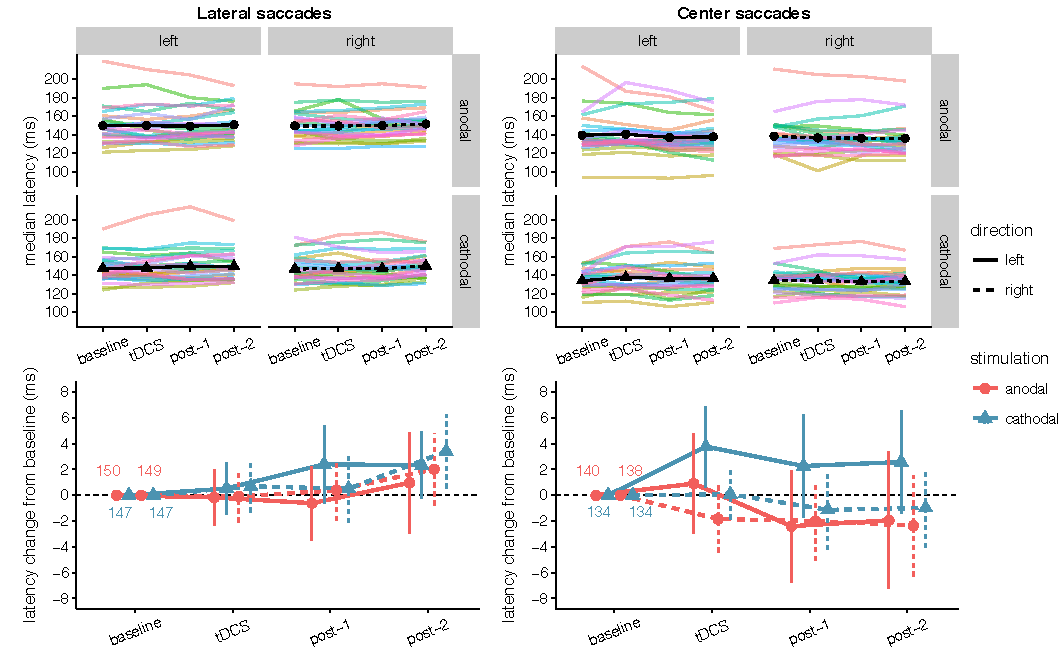
\includegraphics[width=130mm]{sacc_tDCS_files/figures/figure_4_latency} \caption{\textbf{Effects of frontal eye field tDCS on saccade latency.} Data are shown for left vs.~rightward saccades, in the anodal vs.~cathodal session, for four 15-minute time periods: baseline, during tDCS, and after tDCS (post-1 and post-2). \textbf{Top row}: Colored lines show data from individual participants; black lines show the group median. \textbf{Bottom row}: Change in saccade latency after baseline subtraction. Numbers inside the plot axes are the baseline saccade latencies per condition. Error bars show 95\% confidence intervals of the pairwise difference between baseline and each subsequent time period.}\label{fig:fig-latency}
\end{figure}



\begingroup
\setlength{\LTleft}{-20cm plus -1fill}
\setlength{\LTright}{\LTleft}
\small

\begin{longtable}[]{@{}lllllll@{}}
\caption{\label{tab:tab-latency} \textbf{Classical and Bayesian repeated measures ANOVA results for saccade latency}. Factors: \emph{Stimulation} (anodal vs.~cathodal), \emph{Time Period} (during tDCS, post-tDCS {[}0-15 min{]}, post-tDCS {[}0-30 min{]}), \emph{Direction} (saccade to the left vs.~saccade to the right).}\tabularnewline
\toprule
Effect & df & F & \(\eta_{G}^{2}\) & \emph{p} & BF\textsubscript{10} & BF\textsubscript{01}\tabularnewline
\midrule
\endfirsthead
\toprule
Effect & df & F & \(\eta_{G}^{2}\) & \emph{p} & BF\textsubscript{10} & BF\textsubscript{01}\tabularnewline
\midrule
\endhead
\textbf{lateral saccades} & & & & & &\tabularnewline
Stimulation & 1, 25 & 0.80 & .009 & .38 & 0.76 & 1.32\tabularnewline
Stimulation x Direction & 1, 25 & 0.52 & .001 & .48 & 0.22 & 4.56\tabularnewline
Stimulation x Time Period & 2, 50 & 0.40 & .0008 & .67 & 0.074 & 13.5\tabularnewline
Stimulation x Direction x Time Period & 2, 50 & 2.59 & .003 & .085 & 0.18 & 5.64\tabularnewline
\textbf{center saccades} & & & & & &\tabularnewline
Stimulation & 1, 25 & 3.09 & .023 & .091 & 67.2 & 0.015\tabularnewline
Stimulation x Direction & 1, 25 & 1.88 & .006 & .18 & 0.74 & 1.34\tabularnewline
Stimulation x Time Period & 2, 50 & 0.11 & .0002 & .90 & 0.066 & 15.1\tabularnewline
Stimulation x Direction x Time Period & 2, 50 & 1.96 & .001 & .15 & 0.19 & 5.40\tabularnewline
\bottomrule
\end{longtable}

\endgroup

\hypertarget{saccade-latency-distribution}{%
\subsection{Saccade latency distribution}\label{saccade-latency-distribution}}

Because the hypothesized effect on median saccade latency was absent, we conducted an additional exploratory analysis (see \protect\hyperlink{quantile-analysis}{Quantile analysis} in the \protect\hyperlink{sacc_tDCS-methods}{Material and Methods} section) by comparing the entire saccade latency distributions between the anodal and cathodal sessions (Figure \ref{fig:quantiles}). Across the board, saccade latencies in the cathodal session were slightly faster than the anodal session, which is opposite to the hypothesized effect of tDCS on FEF excitability. For lateral saccades, the slowest saccades seem to show the biggest difference in latency between the sessions; for center saccades, differences were most pronounced in the fastest saccades. However, these differences were already present in the baseline block, and appear to be driven by a small number of participants. Overall, effects were never significant in the same direction in more than 12 (out of 26) participants.

\begin{figure}
\includegraphics[width=130mm]{sacc_tDCS_files/figures/figure_5_quantiles} \caption{\textbf{Shift functions of saccade latency distributions under anodal and cathodal tDCS.} Data are shown for left- vs.~rightward saccades for four 15-minute time periods: baseline, during tDCS, and after tDCS (post-1 and post-2). \textbf{Left column}: The x-axis shows saccade latencies for the 9 deciles in the anodal session. The median is plotted as a vertical dashed line. The y-axis shows the difference scores (anodal - cathodal) at each decile. These decile differences express by how much latencies for the cathodal deciles should be \emph{shifted} to match the anodal deciles. Positive differences mean that cathodal saccades had lower latencies than anodal saccades. Error bars show 95\% confidence intervals of the decile differences. \textbf{Right column}: Counts of participants showing significant effects for the difference between anodal and cathodal sessions at each decile. Red/top bars count the number of participants with faster anodal saccade latencies; blue/bottom bars show counts for faster cathodal latencies. 26 participants is the maximum; the exact number for each contrast is superimposed on the bars.}\label{fig:quantiles}
\end{figure}



\hypertarget{saccade-endpoint-deviation}{%
\subsection{Saccade endpoint deviation}\label{saccade-endpoint-deviation}}

No significant effects of tDCS on saccade endpoint deviation were expected, as none were found in \textcite{Kanai2012}. Yet, at first glance the data seem to show that accuracy improved (i.e.~endpoint deviation decreased) with cathodal tDCS (Figure \ref{fig:fig-deviation}). There was a significant and rather large main effect of Stimulation for center saccades, supported by moderate (lateral saccades) to extreme (center saccades) evidence (Table \ref{tab:tab-deviation}). Follow-up one-sample tests for center saccades showed that endpoint deviation only changed significantly from baseline in the cathodal session (\emph{p} = .004, BF\textsubscript{10} = 10.5), not the anodal session (\emph{p} = .34, BF\textsubscript{01} = 3.15).

However, this interpretation is muddled by a difference between anodal and cathodal in the baseline, so before tDCS onset (Figure \ref{fig:fig-deviation}). For center saccades, the difference was in fact larger in the baseline than at any other time period (left: mean difference = -0.11°, 95\% CI = -0.20° -- -0.01°, \emph{p} = .025; right: mean difference = -0.06°, 95\% CI = -0.11° -- 0.00°, \emph{p} = .066). For example, during tDCS, this difference between anodal and cathodal had completely disappeared (left: \emph{M}\textsubscript{anodal} = 0.91° = \emph{M}\textsubscript{cathodal} = 0.91°; right: \emph{M}\textsubscript{anodal} = \emph{M}\textsubscript{cathodal} = 0.72°), as endpoint deviation in the anodal session increased from baseline, while it decreased in the cathodal session, thereby cancelling out the baseline difference. Thus, like in \textcite{Kanai2012}, our results do not appear to support an effect of tDCS on saccade endpoint deviation.

\begin{figure}
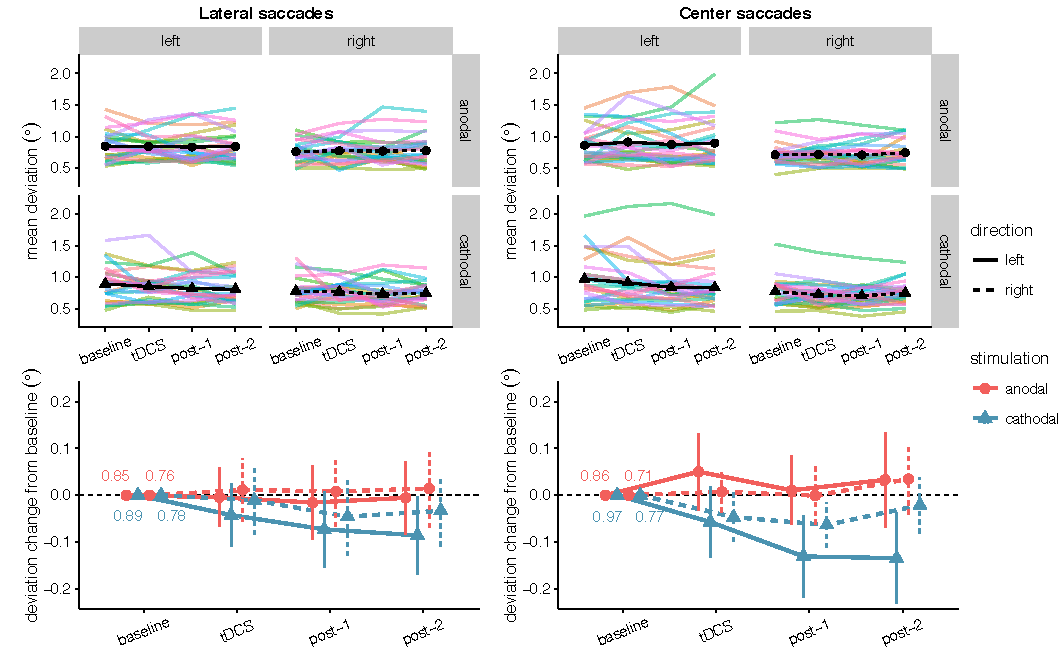
\includegraphics[width=130mm]{sacc_tDCS_files/figures/figure_6_deviation} \caption{\textbf{Effects of frontal eye field tDCS on saccade endpoint deviation.} Data are shown for left vs.~rightward saccades, in the anodal vs.~cathodal session, averaged over four 15-minute time periods: baseline, during tDCS, and after tDCS (post-1 and post-2). \textbf{Top row}: Colored lines show data from individual participants; black lines show the group median. \textbf{Bottom row}: Change in saccade endpoint deviation after baseline subtraction. Numbers inside the plot axes are the baseline saccade endpoint deviations. Error bars show 95\% confidence intervals of the pairwise difference between baseline and each subsequent time period.}\label{fig:fig-deviation}
\end{figure}



\begingroup
\setlength{\LTleft}{-20cm plus -1fill}
\setlength{\LTright}{\LTleft}
\small

\begin{longtable}[]{@{}lllllll@{}}
\caption{\label{tab:tab-deviation} \textbf{Classical and Bayesian repeated measures ANOVA results for saccade endpoint deviation}. Factors: \emph{Stimulation} (anodal vs.~cathodal), \emph{Time Period} (during tDCS, post-tDCS {[}0-15 min{]}, post-tDCS {[}0-30 min{]}), \emph{Direction} (saccade to the left vs.~saccade to the right).}\tabularnewline
\toprule
Effect & df & F & \(\eta_{G}^{2}\) & \emph{p} & BF\textsubscript{10} & BF\textsubscript{01}\tabularnewline
\midrule
\endfirsthead
\toprule
Effect & df & F & \(\eta_{G}^{2}\) & \emph{p} & BF\textsubscript{10} & BF\textsubscript{01}\tabularnewline
\midrule
\endhead
\textbf{lateral saccades} & & & & & &\tabularnewline
Stimulation & 1, 25 & 2.03 & .018 & .17 & 6.64 & 0.15\tabularnewline
Stimulation x Direction & 1, 25 & 0.13 & .001 & .72 & 0.19 & 5.21\tabularnewline
Stimulation x Time Period & 2, 50 & 0.59 & .002 & .56 & 0.084 & 12.0\tabularnewline
Stimulation x Direction x Time Period & 2, 50 & 0.28 & .0003 & .76 & 0.12 & 8.19\tabularnewline
\textbf{center saccades} & & & & & &\tabularnewline
Stimulation & 1, 25 & 10.34 & .070 & .004 & 42,209 & 0.00002\tabularnewline
Stimulation x Direction & 1, 25 & 2.80 & .013 & .11 & 1.69 & 0.59\tabularnewline
Stimulation x Time Period & 2, 50 & 0.61 & .001 & .55 & 0.079 & 12.7\tabularnewline
Stimulation x Direction x Time Period & 2, 50 & 0.59 & .001 & .56 & 0.11 & 8.73\tabularnewline
\bottomrule
\end{longtable}

\endgroup

\hypertarget{saccade-endpoint-variability}{%
\subsection{Saccade endpoint variability}\label{saccade-endpoint-variability}}

Like for saccade endpoint deviation, we had no specific hypotheses on endpoint variability, as \textcite{Kanai2012} obtained no effects. However, like the decrease in endpoint deviation, cathodal tDCS also appeared to decrease saccade endpoint variability (Figure \ref{fig:fig-variability}). For center saccades, there was extreme evidence for inclusion of the main effect of Stimulation in the Bayesian ANOVA, yet the effect only approached significance in the classical ANOVA (Table \ref{tab:tab-variability}). However, while the variability changes in the anodal and cathodal sessions may have differed from each other, follow-up one sample tests showed that neither anodal (\emph{p} = .11, BF\textsubscript{01} = 1.40) nor cathodal (\emph{p} = .23, BF\textsubscript{01} = 2.44) changed significantly from baseline. Thus, saccade endpoint variability also does not seem to be affected by tDCS, conform the findings of \textcite{Kanai2012}.

\begin{figure}
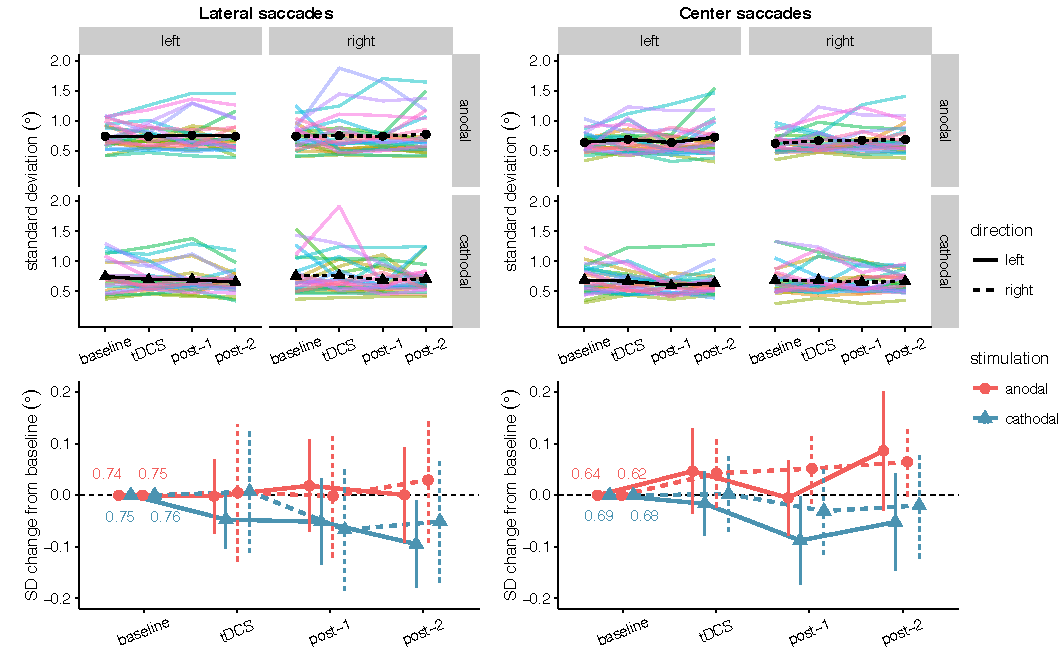
\includegraphics[width=130mm]{sacc_tDCS_files/figures/figure_7_variability} \caption{\textbf{Effects of frontal eye field tDCS on saccade endpoint variability.} Data are shown for left vs.~rightward saccades, in the anodal vs.~cathodal session, averaged over four 15-minute time periods: baseline, during tDCS, and after tDCS (post-1 and post-2). \textbf{Top row}: Colored lines show data from individual participants; black lines show the group median. \textbf{Bottom row}: Change in saccade endpoint variability after baseline subtraction. Numbers inside the plot axes are the baseline saccade endpoint variability values. Error bars show 95\% confidence intervals of the pairwise difference between baseline and each subsequent time period.}\label{fig:fig-variability}
\end{figure}



\begingroup
\setlength{\LTleft}{-20cm plus -1fill}
\setlength{\LTright}{\LTleft}
\small

\begin{longtable}[]{@{}lllllll@{}}
\caption{\label{tab:tab-variability} \textbf{Classical and Bayesian repeated measures ANOVA results for saccade endpoint variability}. Factors: \emph{Stimulation} (anodal vs.~cathodal), \emph{Time Period} (during tDCS, post-tDCS {[}0-15 min{]}, post-tDCS {[}0-30 min{]}), \emph{Direction} (saccade to the left vs.~saccade to the right).}\tabularnewline
\toprule
Effect & df & F & \(\eta_{G}^{2}\) & \emph{p} & BF\textsubscript{10} & BF\textsubscript{01}\tabularnewline
\midrule
\endfirsthead
\toprule
Effect & df & F & \(\eta_{G}^{2}\) & \emph{p} & BF\textsubscript{10} & BF\textsubscript{01}\tabularnewline
\midrule
\endhead
\textbf{lateral saccades} & & & & & &\tabularnewline
Stimulation & 1, 25 & 1.22 & .014 & .28 & 1.63 & 0.61\tabularnewline
Stimulation x Direction & 1, 25 & 0.12 & .0005 & .73 & 0.19 & 5.28\tabularnewline
Stimulation x Time Period & 2, 50 & 1.12 & .003 & .33 & 0.11 & 9.48\tabularnewline
Stimulation x Direction x Time Period & 2, 50 & 0.19 & .0003 & .83 & 0.089 & 11.2\tabularnewline
\textbf{center saccades} & & & & & &\tabularnewline
Stimulation & 1, 25 & 3.89 & .040 & .060 & 145 & 0.007\tabularnewline
Stimulation x Direction & 1, 25 & 0.17 & .001 & .68 & 0.22 & 4.63\tabularnewline
Stimulation x Time Period & 2, 50 & 1.18 & .004 & .32 & 0.11 & 8.89\tabularnewline
Stimulation x Direction x Time Period & 2, 50 & 0.47 & .0007 & .63 & 0.12 & 8.30\tabularnewline
\bottomrule
\end{longtable}

\endgroup

\hypertarget{sacc_tDCS-discussion}{%
\section{Discussion}\label{sacc_tDCS-discussion}}

Given the central role the frontal eye field plays in spatial attention, we wanted to examine whether FEF activity could be reliably influenced through tDCS. As the FEF is involved in initiation of eye movements, we measured latency and accuracy of prosaccades to evaluate the effects of tDCS. Our study was based on earlier work \autocite{Kanai2012}, which reported that anodal tDCS could speed saccades to targets contralateral to the stimulated FEF. To summarize our results, we were unable to replicate the main effect of \textcite{Kanai2012}: anodal tDCS did not decrease the latency of contralateral prosaccades. We also found no effects on saccade accuracy, though neither did \textcite{Kanai2012}.

For saccades back to the center location, Bayesian analyses provided evidence for a differing effect of anodal and cathodal tDCS (regardless of whether saccades were ipsi-/contralateral, or whether they were made during/after stimulation) on all measures we examined: saccade latency, saccade endpoint deviation and saccade endpoint variability. However, in the case of latency and endpoint variability, the corresponding classical analysis was non-significant. Also, follow-up tests (both Bayesian and classical) showed that scores in neither the anodal nor cathodal condition changed significantly from baseline. For endpoint deviation, there was a significant difference between the anodal and cathodal sessions in the baseline, which might have driven the effect. We are therefore hesitant to interpret any of these effects as genuine changes caused by frontal eye field tDCS. Likewise, our shift function analysis painted a complex pattern of differences in the saccade latency distributions for the anodal and cathodal sessions. But these varied highly between individuals and did not seem to exceed the differences that were already present in the baseline block. Collectively, these results do not support an effect of FEF-tDCS on the speed or accuracy of eye movements, and add to a growing body of work that found no results of FEF-tDCS \autocites{Chen2017}{Ball2013}{Ellison2014}, and tDCS in general \autocites{Medina2017}{Voroslakos2018}.

Out of all these results, our null finding for saccade latency is the most surprising. Why did \textcite{Kanai2012} find that anodal tDCS speeded (contralateral) saccades, but we did not? Our study should not be considered a direct replication of \textcite{Kanai2012}, and there are a number of methodological differences between the two. We have tried to enumerate and explain all of them in Table \ref{tab:differences}. Some are clear and simple improvements, such as the increased statistical power, trial count, and eye tracker sampling rate. Others are more ambiguous: of course, each change was made with the aim to increase the size of the tDCS effect, but each change could also be the cause of why we no longer obtain an effect at all. If that is the case, the changes to the stimulation duration and electrode montage would likely have had the most consequences.

\newpage
\pagestyle{empty}
\newgeometry{left=20mm,right=0.5in,top=0.2in,bottom=0.2in} % narrow margins (0.5), bit more at top, adjust table sides
\blandscape
\LTcapwidth=200mm % make caption almost as wide as table
\small

\begin{longtable}[]{@{}llll@{}}
\caption{\label{tab:differences} Methodological differences between \textcite{Kanai2012} and the present study.}\tabularnewline
\toprule
\begin{minipage}[b]{0.14\columnwidth}\raggedright
Difference\strut
\end{minipage} & \begin{minipage}[b]{0.21\columnwidth}\raggedright
Here\strut
\end{minipage} & \begin{minipage}[b]{0.16\columnwidth}\raggedright
\textcite{Kanai2012}\strut
\end{minipage} & \begin{minipage}[b]{0.38\columnwidth}\raggedright
Reason\strut
\end{minipage}\tabularnewline
\midrule
\endfirsthead
\toprule
\begin{minipage}[b]{0.14\columnwidth}\raggedright
Difference\strut
\end{minipage} & \begin{minipage}[b]{0.21\columnwidth}\raggedright
Here\strut
\end{minipage} & \begin{minipage}[b]{0.16\columnwidth}\raggedright
\textcite{Kanai2012}\strut
\end{minipage} & \begin{minipage}[b]{0.38\columnwidth}\raggedright
Reason\strut
\end{minipage}\tabularnewline
\midrule
\endhead
\begin{minipage}[t]{0.14\columnwidth}\raggedright
Sample size and design\strut
\end{minipage} & \begin{minipage}[t]{0.21\columnwidth}\raggedright
n=26, within-subject design\strut
\end{minipage} & \begin{minipage}[t]{0.16\columnwidth}\raggedright
n=32, between-subject design\strut
\end{minipage} & \begin{minipage}[t]{0.38\columnwidth}\raggedright
More observations per cell, less influence of between-subject variability\strut
\end{minipage}\tabularnewline
\begin{minipage}[t]{0.14\columnwidth}\raggedright
FEF localization\strut
\end{minipage} & \begin{minipage}[t]{0.21\columnwidth}\raggedright
MRI-guided per individual\strut
\end{minipage} & \begin{minipage}[t]{0.16\columnwidth}\raggedright
Group MRI coordinate\strut
\end{minipage} & \begin{minipage}[t]{0.38\columnwidth}\raggedright
More power \autocite{Sack2009}\strut
\end{minipage}\tabularnewline
\begin{minipage}[t]{0.14\columnwidth}\raggedright
tDCS: duration\strut
\end{minipage} & \begin{minipage}[t]{0.21\columnwidth}\raggedright
15 minutes\strut
\end{minipage} & \begin{minipage}[t]{0.16\columnwidth}\raggedright
10 minutes\strut
\end{minipage} & \begin{minipage}[t]{0.38\columnwidth}\raggedright
More trials during stimulation; possibly increase tDCS effect\strut
\end{minipage}\tabularnewline
\begin{minipage}[t]{0.14\columnwidth}\raggedright
tDCS: location\strut
\end{minipage} & \begin{minipage}[t]{0.21\columnwidth}\raggedright
Right FEF\strut
\end{minipage} & \begin{minipage}[t]{0.16\columnwidth}\raggedright
Right or left FEF\strut
\end{minipage} & \begin{minipage}[t]{0.38\columnwidth}\raggedright
Right FEF is dominant \autocite{Duecker2015}\strut
\end{minipage}\tabularnewline
\begin{minipage}[t]{0.14\columnwidth}\raggedright
tDCS: montage\strut
\end{minipage} & \begin{minipage}[t]{0.21\columnwidth}\raggedright
FEF, contralateral forehead\strut
\end{minipage} & \begin{minipage}[t]{0.16\columnwidth}\raggedright
FEF, ipsilateral shoulder\strut
\end{minipage} & \begin{minipage}[t]{0.38\columnwidth}\raggedright
Decreased interelectrode distance increases effect \autocites{Moliadze2010}{Opitz2015}. Resembles canonical motor cortex montage\strut
\end{minipage}\tabularnewline
\begin{minipage}[t]{0.14\columnwidth}\raggedright
tDCS: conductive medium\strut
\end{minipage} & \begin{minipage}[t]{0.21\columnwidth}\raggedright
Ten20 conductive paste\strut
\end{minipage} & \begin{minipage}[t]{0.16\columnwidth}\raggedright
Saline soaked sponges\strut
\end{minipage} & \begin{minipage}[t]{0.38\columnwidth}\raggedright
Uniform electrode-skin contact, no risk of excess/leaking saline\strut
\end{minipage}\tabularnewline
\begin{minipage}[t]{0.14\columnwidth}\raggedright
Number of saccades per condition\strut
\end{minipage} & \begin{minipage}[t]{0.21\columnwidth}\raggedright
180 (per 15 minutes)\strut
\end{minipage} & \begin{minipage}[t]{0.16\columnwidth}\raggedright
40 (per 10 minutes)\strut
\end{minipage} & \begin{minipage}[t]{0.38\columnwidth}\raggedright
More robust estimates within each participant\strut
\end{minipage}\tabularnewline
\begin{minipage}[t]{0.14\columnwidth}\raggedright
Task: stimulus overlap\strut
\end{minipage} & \begin{minipage}[t]{0.21\columnwidth}\raggedright
No overlap of fixation and target\strut
\end{minipage} & \begin{minipage}[t]{0.16\columnwidth}\raggedright
Fixation point always on\strut
\end{minipage} & \begin{minipage}[t]{0.38\columnwidth}\raggedright
Possibility to analyze saccades back to fixation (center)\strut
\end{minipage}\tabularnewline
\begin{minipage}[t]{0.14\columnwidth}\raggedright
Task: placeholders\strut
\end{minipage} & \begin{minipage}[t]{0.21\columnwidth}\raggedright
None\strut
\end{minipage} & \begin{minipage}[t]{0.16\columnwidth}\raggedright
Target location marked with placeholders\strut
\end{minipage} & \begin{minipage}[t]{0.38\columnwidth}\raggedright
Spatial uncertainty might create more room for improvements in accuracy with tDCS\strut
\end{minipage}\tabularnewline
\begin{minipage}[t]{0.14\columnwidth}\raggedright
Task: inter-stimulus interval\strut
\end{minipage} & \begin{minipage}[t]{0.21\columnwidth}\raggedright
Exponential distribution: mean 500 ms, bounds 300-3000 ms\strut
\end{minipage} & \begin{minipage}[t]{0.16\columnwidth}\raggedright
Normal distribution, bounds: 300-700 ms\strut
\end{minipage} & \begin{minipage}[t]{0.38\columnwidth}\raggedright
Temporally more unpredictable target onsets\strut
\end{minipage}\tabularnewline
\begin{minipage}[t]{0.14\columnwidth}\raggedright
Eye tracker: sampling rate\strut
\end{minipage} & \begin{minipage}[t]{0.21\columnwidth}\raggedright
1000 Hz\strut
\end{minipage} & \begin{minipage}[t]{0.16\columnwidth}\raggedright
250 Hz\strut
\end{minipage} & \begin{minipage}[t]{0.38\columnwidth}\raggedright
More adequate resolution for small effects\strut
\end{minipage}\tabularnewline
\begin{minipage}[t]{0.14\columnwidth}\raggedright
Eye tracker: saccade threshold\strut
\end{minipage} & \begin{minipage}[t]{0.21\columnwidth}\raggedright
\textgreater{} 30 °/s velocity \& \textgreater{} 8000 °/s\textsuperscript{2} acceleration\strut
\end{minipage} & \begin{minipage}[t]{0.16\columnwidth}\raggedright
\textgreater{} 26.8 °/s velocity\strut
\end{minipage} & \begin{minipage}[t]{0.38\columnwidth}\raggedright
(Eyelink standards)\strut
\end{minipage}\tabularnewline
\bottomrule
\end{longtable}

\newpage
\normalsize
\elandscape
\restoregeometry % revert to normal margins set with memoir
\pagestyle{\defstyle}

We increased the stimulation duration from 10 to 15 minutes, in order to have more trials during tDCS and possibly a larger neural effect. But longer stimulation durations do not necessarily scale linearly with the effect of tDCS. For example, changing the stimulation duration from 20 to 26 minutes changed the effect of anodal tDCS on motor-evoked potentials from excitatory to inhibitory \autocite{Monte-Silva2013}. In addition, we changed the location of the second electrode from the shoulder to the forehead, to more closely resemble the canonical montage used in motor cortex tDCS, and because decreasing the inter-electrode distance can enhance the effect of tDCS \autocite{Moliadze2010}. However, next to applying tDCS over the right frontal eye field, it is possible that we now also delivered opposite polarity stimulation to left anterior frontal brain structures. In addition, the exact montage determines to a large extent which brain structures will be in the path of the current---not just those directly under the electrodes, but also those in between \autocite{Opitz2015}, as well as distant structures that are anatomically connected \autocite{Wokke2015}.

We stress that \textcite{Kanai2012} also did an experiment with a different electrode montage, in which they delivered bilateral tDCS by placing the anode over the left or right FEF and the cathode over the other FEF (counterbalanced across participants). This montage produced a similar effect, but actually was more effective: tDCS now also speeded saccades contralateral to the anode, but the effect was bigger (7.8 vs.~6.4 ms), and follow-up tests revealed that it was significant at more time points (from 0--30 min after tDCS vs.~only 10--20 minutes after tDCS). Nevertheless, we chose to go with a unilateral montage, to be sensitive to possible lateralization of effects. With a bilateral montage, it is impossible to tell whether the effect stems from anodal tDCS to one FEF, cathodal tDCS to the other FEF, or from both at the same time.

Our study was not the first that found no effect of tDCS on saccade latency. \textcite{Chen2017} also set out to replicate this effect, and were also unsuccessful. Like ours, their study was not a direct replication and differed from the protocol used by \textcite{Kanai2012} in multiple ways. Specifically, they did not perform MRI-based neuronavigation, and postulated that this might have been the prime reason for why they did not find any effects of tDCS. Although they did place the second electrode on the shoulder, like \textcite{Kanai2012}, \textcite{Chen2017} also suggest that future studies place it on the left forehead (following the conventional stimulation setup for the motor cortex). Strikingly, our study followed both suggestions (even though our data were collected before their study was published), so it appears these two factors were not responsible for the discrepant results after all.

In addition to the methods, there was also a difference between these studies in average saccade latency. In our study, participants were on average faster (\textasciitilde{}150 ms for lateral saccades) than in \textcite{Kanai2012} (\textasciitilde{}180 ms). The average center saccade latency was faster still (\textasciitilde{}135 ms), presumably because the target location was known beforehand in this case. This could be because of changes to the task we made (see Table \ref{tab:differences}), specifically to have no overlap between target and fixation, and to have no placeholders at the target locations. Both of these are known to reduce saccade latency \autocite{Sumner2011}. Curiously, \textcite{Chen2017} made similar task modifications, but yet obtained not faster but slower saccade latencies (\textasciitilde{}200 ms).

Although our saccade latencies were faster in the baseline block already, which was thus clearly unrelated to tDCS, this could have diminished the effectiveness of tDCS. The relatively fast latencies could be due to increased inhibition of fixation and an increased proportion of very fast saccades, which rely more on other structures like the superior colliculus \autocites{Munoz1992}{Munoz2002} than the frontal eye field. The frontal eye field itself is also not functionally homogeneous: it contains many types of cells \autocite{Lowe2017}, not just neurons that initiate eye movements, but also those that promote fixation. Even if the frontal eye field was effectively stimulated, there may have been no net effect of tDCS, as the opposing actions of the different cell types could cancel each other out.

Relatedly, the fast saccade latencies could indicate that there was little room for improvement left, and that this task was thus too simple to fully recruit the frontal eye fields. The frontal eye fields are more involved in more effortful tasks, and FEF activity most strongly reflects top-down control \autocite{Schafer2011}. Lesions of the frontal eye field also impact antisaccades and memory-guided saccades more heavily than simple prosaccades \autocite{Rivaud1994}. However, other FEF-tDCS studies that have used more complex tasks like visual search \autocites{Ball2013}{Ellison2017} or the antisaccade task \autocite{Chen2017} still found no effects of tDCS.

Perhaps the explanation is also less interesting: the effect could have simply been too small to detect. In \textcite{Kanai2012} the reductions in latency produced by tDCS were already fairly modest, especially considering that pioneering studies tend to overestimate effect sizes \autocite{Ioannidis2008}. The neural effects of tDCS itself may also be smaller than anticipated, as recent studies found that the strength of the electric field in the brain is at the lower bound for it to be physiologically effective \autocites{Huang2017}{Voroslakos2018}. As tDCS effects are increasingly viewed as state-dependent, non-linear \autocites{Fertonani2017}{Bestmann2014} and subject to individual variability \autocites{Li2015b}{Krause2014}, it might be necessary for future studies to use much larger sample sizes \autocite{Minarik2016}. It is also vital that future studies employ a sham condition, as there is no a priori guarantee that the anodal/cathodal dichotomy holds for other brain areas \autocite{Bestmann2017} like the frontal eye field.

Such large, well-controlled and more informed \autocite{Polania2018} studies will be necessary to more clearly establish the boundary conditions of tDCS effects, especially when extending the technique to new brain areas. In the present work, we tried to do so by performing a conceptual replication of the first frontal eye field tDCS study \autocite{Kanai2012}. As tDCS did not reliably affect saccade latency or accuracy, we conclude that the efficacy of frontal eye field tDCS remains uncertain.

\hypertarget{AB-tDCS-EEG}{%
\chapter{Effects of tDCS on the attentional blink revisited: A statistical evaluation of a replication attempt}\label{AB-tDCS-EEG}}

\chaptermark{Replicating tDCS effects on the attentional blink}

\vspace*{\fill}

\begin{center}\rule{0.5\linewidth}{\linethickness}\end{center}

\small

\noindent
\emph{This chapter is in preparation as}: Reteig, L. C., Newman, L. A., Ridderinkhof, K. R., \& Slagter, H. A. (n.d.). Effects of tDCS on the attentional blink revisited: A statistical evaluation of a replication attempt.
\newpage
\normalsize

\begin{abstract}
The attentional blink (AB) phenomenon reveals a bottleneck of human information processing: the second of two targets is often missed when they are presented in rapid succession among distractors. A recent study by London \& Slagter (\emph{Journal of Cognitive Neuroscience}, \emph{27}, 2382--93, 2015) showed that the size of the AB can be changed by applying transcranial direct current stimulation (tDCS) over the left dorsolateral prefrontal cortex (lDLPFC). Although AB size at the group level remained unchanged, the effects of anodal and cathodal tDCS were negatively correlated: if a given individual's AB size decreased from baseline during anodal tDCS, their AB size would increase during cathodal tDCS, and vice versa. Here, we attempted to replicate this finding. Like London \& Slagter, we found no group effects of tDCS, but also no longer found a significant negative correlation. We present a series of statistical measures of replication success, all of which confirm that both studies are not in agreement. First, the correlation here is significantly smaller than a conservative estimate of the original correlation. Second, the difference between the correlations is greater than expected due to sampling error, and our data are more consistent with a zero-effect than with the original estimate. Finally, the overall effect when combining both studies is small and not significant. Our findings thus indicate that the effects of lDPLFC-tDCS on the AB are less substantial than suggested by London \& Slagter (2015). Although this should be quite a common scenario, negative findings can be difficult to interpret and are still under-represented in the brain stimulation and cognitive neuroscience literatures. An auxiliary goal of this chapter is therefore to provide a tutorial for other researchers, to maximize the evidential value from negative findings.
\end{abstract} \newpage

\hypertarget{AB_tDCS-introduction}{%
\section{Introduction}\label{AB_tDCS-introduction}}

The \emph{attentional blink} (AB) phenomenon clearly demonstrates that our capacity to process incoming information is easily overwhelmed. The AB occurs when two targets are embedded in a rapidly presented stream of distractors \autocites{Raymond1992}[for reviews, see][]{Dux2009}{Martens2010}. The first target (T1) is usually reported with little difficulty. When there is a longer lag between the two targets \autocite[\textgreater{} 500 ms;][]{MacLean2012}, accuracy for the second target (T2) can be on par with the first. However, for shorter lags, T2 is most often missed---as if the attentional system momentarily faltered (``blinked'').

While the AB might seem to be a fundamental bottleneck, it can under some circumstances be overcome. For example, the size of the AB can be reduced by distracting activities \autocites{Olivers2005}{Olivers2006}{Thomson2015a}, or after following an intensive mental training program \autocite{Slagter2007}. Others have tried to use non-invasive brain stimulation \autocite{Dayan2013} as a means to influence the AB. Several studies have shown that repetitive transcranial magnetic stimulation (TMS) can improve target perception in AB tasks \autocites{Cooper2004}{Arasanz2012}{Esterman2017}. Yet, as TMS did not show a differential effect for targets presented at shorter or longer lags, it did not affect the AB itself.

Transcranial direct current stimulation (tDCS) is another brain stimulation technique that has gained traction in the past two decades. In tDCS, an electrical current flows between an anodal and cathodal electrode, which can affect the excitability of the underlying cortex \autocite{Gebodh2019a}. Anodal stimulation generally enhances cortical excitability, while cathodal stimulation may have an inhibitory effect \autocites{Nitsche2000}{Nitsche2001} (though note that this does not hold in all cases \autocite{Parkin2018}, and the underlying physiology is complex \autocites{Bikson2019}{Liu2018}{Stagg2018}).

\textcite{London2015} were the first to examine the effects of tDCS on the AB. They applied anodal and cathodal tDCS over the left dorsolateral prefrontal cortex (lDPLFC, with the other electrode on the right forehead)---one of the core brain areas implicated in the AB \autocites{Slagter2010}{Hommel2006}. At the group level, tDCS did not appear to have any effects on AB size. However, anodal and cathodal tDCS did appear to systematically affect the AB within individuals, as their effects were negatively correlated. For a given individual, this negative correlation implies that when AB size increased (compared to a baseline measurement) during anodal tDCS, AB size would decrease during cathodal tDCS (or vice versa).

London and Slagter's \autocite*{London2015} findings mesh well with earlier literature showing large individual differences in both the AB \autocite{Willems2016} and effects of tDCS \autocite{Krause2014}. However, it remains the only tDCS study of the AB to date. Also, the negative correlation between the effects of anodal and cathodal tDCS was based on an exploratory analysis. We thus decided to conduct another study aiming to replicate this finding.

To foreshadow our results, like \textcite{London2015}, we do not find a group effect of tDCS on the AB. However, the correlation between the effects of anodal and cathodal tDCS was also not significant. Although this indicates that the two studies may differ, a failure to reject the null hypothesis by itself does not tell us much \autocite{Harms2018}: it is crucial to also take measures of the uncertainty and effect size in both studies into account \autocite{Simonsohn2015}.

Therefore, we employ a number of statistical methods to maximize the evidential value in these two studies. We ask three questions that all aim to evaluate to what extent the present study is a successful replication \autocites{Zwaan2018}[cf.][]{Camerer2018}{OSC2015} of \textcite{London2015}. First, while the effect in our study was not significant, there might still be a meaningful effect that is simply smaller than anticipated. Therefore, we used equivalence testing \autocite{Lakens2018} to answer the question ``\emph{is the correlation in study 2 significantly small?}''. Second, although our result differs from \textcite{London2015}, it could still be more consistent with their findings than with alternative explanations. So in addition, we asked ``\emph{are the correlations consistent across studies 1 and 2?}'', and aimed to answer this question using prediction intervals \autocites{Spence2016}{Patil2016} and replication Bayes factors \autocites{Wagenmakers2016}{Verhagen2014}. Finally, it could be that the effect in our study alone is not sufficiently large, but the overall effect based on both studies is. This raises the question ``\emph{is the effect significant when combining study 1 and 2?}'', which we addressed through meta-analysis \autocites{Quintana2015}{Goh2016} and by pooling the data.

These questions address issues of reproducibility that are currently faced by many in the brain stimulation field \autocite{Heroux2017}, and in the cognitive neuroscience community at large \autocites{Munafo2017}{Huber2019}. Therefore, aside from our focus on tDCS and the AB, an auxiliary goal of this chapter is to provide a tutorial on the statistical evaluation of replication studies. We hope this may prove useful to other researchers who find themselves in similar situations.

\hypertarget{AB_tDCS-methods}{%
\section{Materials and Methods}\label{AB_tDCS-methods}}

\hypertarget{AB_tDCS-participants}{%
\subsection{Participants}\label{AB_tDCS-participants}}

Fourty-eight participants took part in total, 8 of whom were excluded after the first session. One participant was excluded as a precaution because they developed an atypical headache after the first session, and we could not rule out this was related to the tDCS. Another stopped responding to our requests to schedule the second session. The remaining six participants were excluded because their mean T1 accuracy in the first session was too low, which would leave too few trials to analyze, because our T2 accuracy measure included only trials in which T1 was seen. We used a cut-off of 63\% T1 accuracy as an exclusion criterium, which was two standard deviations below the mean of a separate pilot study (n = 10).

This left a final sample of 40 participants (29 female, mean age = 20.94, \emph{SD} = 2.45, range = 18--28). This sample size was determined a priori to slightly exceed \textcite{London2015} (n = 34).

The experiment and recruitment took place at the University of Amsterdam. All procedures for this study were approved by the ethics review board of the Faculty for Social and Behavioral Sciences, and complied with relevant laws and institutional guidelines. All participants provided their written informed consent and were compensated with course credit or €10 per hour (typically €65 for completing two full sessions).

\hypertarget{AB_tDCS-procedure}{%
\subsection{Procedure}\label{AB_tDCS-procedure}}

The study procedures were identical to \textcite{London2015}: participants received anodal and cathodal tDCS in separate sessions (Figure \ref{fig:AB-tDCS-fig-procedure}), which typically took place exactly one week apart (cf.~minimum of 48 hours in \textcite{London2015}). The time in between served to keep the sessions as similar as possible, and to minimize the risk of tDCS carry-over effects. 18 participants received anodal tDCS in the first session and cathodal tDCS in the second, and vice versa for the remaining 22 participants.

\begin{figure}
\centering
\includegraphics{AB_tDCS_files/figures/figure_1_procedure.pdf}
\caption{\label{fig:AB-tDCS-fig-procedure}\textbf{Experimental design}. After a baseline block without stimulation, participants performed the attentional blink task during 20 minutes of anodal (red) or cathodal (blue) tDCS, followed by a post-test block (also without stimulation). The second session (typically 7 days later) was identical, except that the tDCS polarity was reversed.}
\end{figure}

First, participants experienced the sensations induced by tDCS in a brief trial stimulation (see the \protect\hyperlink{AB_tDCS-tDCS}{tDCS} section). Next, participants completed 20 practice trials of the task (see the \protect\hyperlink{AB_tDCS-task}{Task} section). For the main portion of the experiment, participants performed three blocks of the task (Figure \ref{fig:AB-tDCS-fig-procedure}): before tDCS (\emph{baseline}), during anodal/cathodal tDCS (\emph{tDCS}), and after tDCS (\emph{post}). Finally, after completing the three blocks, participants filled in a questionnaire on tDCS-related adverse effects (see Table \ref{tab:tab-AB-tDCS-AE} and Figure \ref{fig:fig-AB-tDCS-AE} in Appendix \ref{AB-tDCS-supplement}).

Within each block of the task, participants took a self-timed break every 50 trials (\textasciitilde{}5 minutes); between the blocks, the experimenter walked in. Participants performed the task for exactly 20 minutes during the \emph{baseline} and \emph{post} blocks. During the \emph{tDCS} block, the task started after the 1-minute ramp-up of the current was complete, and continued for 21 minutes (constant current, plus 1-minute of ramp-down).



\hypertarget{AB_tDCS-task}{%
\subsection{Task}\label{AB_tDCS-task}}

The attentional blink task (Figure \ref{fig:AB-tDCS-fig-task}) was almost identical to the one used in \textcite{London2015} and \textcite{Slagter2013}, which in turn was based on a task designed by \textcite{Dux2008}. A rapid serial visual presentation stream of 15 letters (cf.~17 letters in \textcite{London2015}) was shown on each trial, using Presentation software (Neurobehavioral Systems, Inc.). Each letter was displayed for 91.7 ms (11 frames at 120 Hz) on a dark gray background. The letters were presented in font size 40 (font: Courier New) at a viewing distance of 90 cm. On each trial, the letters were randomly sampled without replacement from the alphabet, excluding the letters I, L, O, Q, U and V, as they were too similar to each other. All distractor letters were mid-gray, whereas T1 and T2 were colored. T1 was red and always appeared at position 5 in the stream. T2 was green and followed T1 after either 2 distractors (\emph{lag 3}) or 7 distractors (\emph{lag 8}) (cf.~lags 2, 4 and 10 in \textcite{London2015}).

The letter stream was preceded by a fixation cross (same color as the letters) presented for 1750 ms (cf.~480 ms in \textcite{London2015}) and followed by another fixation cross (cf.~none in \textcite{London2015}). Finally, the participant was prompted to type in (using a standard keyboard) the letter they thought was presented as T1 (``Which letter was red?''), followed by T2 (``Which letter was green?'').

Trial duration varied slightly because both the T1 and T2 response questions were self-paced, so some participants completed more trials than others depending on their response times. On average, participants completed 130 short lag trials (\emph{SD} = 17; range = 78--163) and 65 long lag trials (\emph{SD} = 9; range = 39--87) per 20-minute block.

\begin{figure}
\centering
\includegraphics{AB_tDCS_files/figures/figure_2_task.pdf}
\caption{\label{fig:AB-tDCS-fig-task}\textbf{Attentional blink task}. Participants viewed rapid serial visual presentation streams of 15 letters, all of which were distractors (gray letters) except for T1 and T2. T1 was presented in red at position 5; T2 was presented in green and followed T1 after 2 distractors (\emph{lag 3}, inside the AB window) or 7 distractors (\emph{lag 8}, outside the AB window). At the end of the trial, participants reported the identity of T1 and then T2 (self-paced).}
\end{figure}



\hypertarget{AB_tDCS-tDCS}{%
\subsection{tDCS}\label{AB_tDCS-tDCS}}

Transcranial direct current stimulation was delivered online (i.e.~during performance of the attentional blink task) using a DC-STIMULATOR PLUS (NeuroCare Group GmbH). The current was ramped up to 1 mA in 1 minute, stayed at 1 mA for 20 minutes, and was ramped down again in 1 minute.

One electrode was placed at F3 (international 10-20 system) to target the lDLPFC; the other was placed over the right forehead, centered above the eye (approximately corresponding to position Fp2). Both electrodes were 5 x 7 cm in size (35 cm\textsuperscript{2}), leading to a current density of 0.029 mA/cm\textsuperscript{2}. The montage and tDCS parameters are identical to \textcite{London2015}, the only exception being the conductive medium. We used Ten20 conductive paste (Weaver and Company), because it was easier to apply concurrently with the EEG equipment (see the \protect\hyperlink{AB_tDCS-EEGdata}{EEG} section); \textcite{London2015} used saline solution as a conductive medium, together with rubber straps to keep the electrodes in place.

Participants received either anodal tDCS (anode on F3, cathode on right forehead) or cathodal tDCS (cathode on F3, anode on right forehead) in separate sessions. The procedure was double-blinded: both the participant and the experimenters were unaware which polarity was applied in a given session. The experimenter loaded a stimulation setting on the tDCS device (programmed by someone not involved in data collection), without knowing whether it was mapped to anodal or cathodal tDCS. In the second session, the experimenter loaded a second setting mapped to the opposite polarity (half the dataset), or simply connected the terminals of the device to the electrodes in the opposite way.

At the start of the experiment, participants received a brief trial stimulation, based on which they decided whether or not they wanted to continue with the rest of the session. The experimenter offered to terminate the experiment in case tDCS was experienced as too uncomfortable, but none of the participants opted to do so. For the trial stimulation, the current was ramped up to 1 mA in 45 seconds, stayed at 1 mA for 15 seconds, and was ramped down again in 45 seconds.

\hypertarget{AB_tDCS-EEGdata}{%
\subsection{EEG}\label{AB_tDCS-EEGdata}}

We also recorded EEG during all three task blocks. Originally, we aimed to analyze the EEG data to obtain a neurophysiological correlate of the individual differences in response to tDCS \autocites{Krause2014}{Li2015b}{Harty2017}. However, since we did not replicate the behavioral effect in \textcite{London2015}, we refrained from further analysis of the EEG data. Instead, we are making the EEG data publicly available \href{https://doi.org/10.18112/openneuro.ds001810.v1.1.0}{on the OpenNeuro platform} \autocite{Reteig2019_data}. The dataset is formatted according to the new Brain Imaging Data Structure (BIDS) standard \autocite{Gorgolewski2016} for EEG \autocite{Pernet2018}, to facilitate re-use. We include the raw data, as well as the fully preprocessed data and the MATLAB code that generated it.

\hypertarget{data-analysis}{%
\subsection{Data analysis}\label{data-analysis}}

Data were analyzed using R \autocite[Version 3.5.1;][]{R-base}\footnote{We, furthermore, used the R-packages \emph{BayesFactor} \autocite[Version 0.9.12.4.2;][]{R-BayesFactor}, \emph{broom} \autocite[Version 0.5.1;][]{R-broom}, \emph{cowplot} \autocite[Version 0.9.99;][]{R-cowplot}, \emph{emmeans} \autocite[Version 1.3.0;][]{R-emmeans}, \emph{here} \autocite[Version 0.1;][]{R-here}, \emph{kableExtra} \autocite[Version 1.1.0;][]{R-kableExtra}, \emph{knitr} \autocite[Version 1.21;][]{R-knitr}, \emph{papaja} \autocite[Version 0.1.0.9842;][]{R-papaja}, \emph{psychometric} \autocite[Version 2.2;][]{R-psychometric}, \emph{pwr} \autocite[Version 1.2.2;][]{R-pwr}, and \emph{tidyverse} \autocite[Version 1.2.1;][]{R-tidyverse}.} from within RStudio \autocite[Version 1.1.463;][]{RStudio2016}.

\hypertarget{group-level-analysis}{%
\subsubsection{Group-level analysis}\label{group-level-analysis}}

Repeated measures ANOVAs were conducted on T1 accuracy (percentage of trials where T1 was reported correctly) and T2\textbar{}T1 accuracy (percentage of trials where T2 was reported correctly, out of the subset of T1-correct trials) using the \emph{afex} package \autocite[Version NA;][]{R-afex}. The same factors were included for both repeated measures ANOVAs, following \textcite{London2015}: Lag (3, 8), Block (baseline, tDCS, post), Stimulation (anodal, cathodal), and the between-subject factor Session order (anodal tDCS in the first session vs.~cathodal tDCS in the first session). Effect sizes are reported as generalized eta-squared (\(\hat{\eta}^2_G\)) \autocite{Bakeman2005}. Greenhouse-Geisser-adjusted degrees of freedom (\(\mathit{df}^{GG}\)) and p-values are reported as a correction for sphericity violations.

\hypertarget{AB_tDCS-ind-diffs}{%
\subsubsection{Individual differences analysis}\label{AB_tDCS-ind-diffs}}

We reproduced the analysis behind Figure 4 of \textcite{London2015}, which showed a differential effect of anodal vs.~cathodal tDCS at the individual participant level. First, we calculated AB magnitude by subtracting T2\textbar{}T1 accuracy at lag 3 from T2\textbar{}T1 accuracy at lag 8. Next, change scores were created by subtracting AB magnitude in the \emph{baseline} block from the \emph{tDCS} and the \emph{post} blocks, respectively. The change scores in the anodal and cathodal session were then correlated to each other. Again following \textcite{London2015}, we computed a partial correlation (using the \emph{ggm} package \autocite[Version NA;][]{R-ggm}), attempting to adjust for variance due to Session order.

\hypertarget{AB_tDCS-rep-analyses}{%
\subsubsection{Replication analyses}\label{AB_tDCS-rep-analyses}}

In contrast to \textcite{London2015}, the analysis described in the previous section did not produce a significant correlation in our dataset. Therefore, we conducted five follow-up analyses that aim to quantify to what extent our results (do not) replicate \textcite{London2015}. These all provide a complementary perspective on this question. First, we performed an \protect\hyperlink{eq}{equivalence test} (1) to assess whether the effect in the present study was significantly smaller than in \textcite{London2015}. While this procedure is more focused on hypothesis testing, we also constructed \protect\hyperlink{pi}{prediction intervals} (2) to capture the range of effect sizes we can expect in a replication of \textcite{London2015}. Both of these procedures are based on frequentist statistics, which cannot directly quantify the amount of evidence for a (null) hypothesis. Therefore, we also computed a \protect\hyperlink{repBF}{replication Bayes factor} (3) that expresses whether the data in the present study are more likely under the null hypothesis that the effect is absent, vs.~the alternative hypothesis that the effect is comparable to \textcite{London2015}. Finally, we directly combined both studies and estimated the size of the overall effect, through \protect\hyperlink{meta}{meta-analysis} (4) of both correlations, and by computing a new correlation on the \protect\hyperlink{pool}{pooled dataset} (5). More details on each analysis can be found in the following sections, and the provided online resources.

\hypertarget{eq}{%
\paragraph{Equivalence tests}\label{eq}}

Equivalence tests can be used to test for the \emph{absence} of an effect of a specific size \autocite[see][ for a tutorial]{Lakens2018}. Usually, the effect size used for the test is the smallest effect size of interest (the SESOI). Typically, equivalence tests are two one-sided tests: one test of the null hypothesis that the effect exceeds the upper equivalence bound (positive SESOI), and one that the effect exceeds the lower equivalence bound (negative SESOI). However, a one-sided test is more appropriate here: \textcite{London2015} found that the effects of anodal and cathodal tDCS were anticorrelated, so we are only interested in negative effect sizes. This is known as an inferiority test \autocite{Lakens2018}.

We follow the ``small telescopes'' \autocite{Simonsohn2015} approach to set the SESOI to \(r_{33\%}\): the correlation that \textcite{London2015} had 33\% power to detect. The reasoning behind this approach is that it is difficult to prove that an effect does not exist at all, but easier to show that it is surprisingly small. An equivalence test can suggest that the effect is unlikely to exceed \(r_{33\%}\), such that the odds to detect it were stacked at least 2:1 against \textcite{London2015}. That would not mean the effect does not exist at all, but it would mean the original evidence for the effect is not very convincing, as ``too small a telescope'' (in this case, an inadequate sample size) was used to reliably detect it.

There are many possible specifications of the SESOI, none of which are necessarily wrong or right \autocite{Lakens2018}. We favored the ``small telescopes'' approach because it constitutes a relatively strict test---\(r_{33\%}\) is much smaller than the original correlation in \textcite{London2015}. Because the observed correlation in \textcite{London2015} could have overestimated the true correlation, it is prudent to set the SESOI to be smaller. Furthermore, the approach was specifically designed to evaluate replication results \autocite{Simonsohn2015}, and has been used previously in large-scale replication studies \autocite[e.g.][]{Camerer2018}.

We conducted an inferiority test using the \emph{TOSTER} package \autocite[Version NA;][]{R-TOSTER} against the null hypothesis that the correlation coefficient in the present study is at least as negative as \(-r_{33\%}\). At a standard alpha level of 0.05, the test is significant if the 90\% confidence interval around the observed correlation does not contain \(r_{33\%}\). This would mean that the observed correlation should be considered ``statistically inferior'', as it is then significantly smaller (i.e.~less negative) than \(-r_{33\%}\).

\hypertarget{pi}{%
\paragraph{Prediction interval}\label{pi}}

Prediction intervals contain a range of values we can expect a new observation to fall within. In our case, the observation of interest is the correlation between the effects of anodal and cathodal tDCS. This correlation is estimated based on a sample, and is thus subject to sampling error: any two estimates of the correlation will almost never be exactly the same. Prediction intervals aim to quantify how dissimilar two estimates can be before we should be surprised.

Here, we construct a prediction interval around the original estimate of the correlation in \textcite{London2015}. This prediction interval contains the range of correlation coefficients we can expect to see in the present study, given the results of \textcite{London2015}. The width of the interval depends on the sample sizes of both studies, as larger samples will reduce variation in the estimates, leading to smaller prediction intervals \autocite{Patil2016}.

If the original study were replicated 100 times, 95 of the observed correlation coefficients would fall within the 95\% prediction interval \autocite{Patil2016}. Note that this definition is related to, but different from, a \emph{confidence interval}, which quantifies uncertainty about the (unknown) true correlation in the population (95 out of every hundred constructed 95\% confidence intervals contain the true population parameter). Because prediction intervals concern the next single observation, they make a more specific claim, and will be wider than confidence intervals.

We calculated a 95\% prediction interval for correlations, following \textcite{Spence2016}, using the \emph{predictionInterval} package \autocite[Version NA;][]{R-predictionInterval}.

\hypertarget{repBF}{%
\paragraph{Replication Bayes factor}\label{repBF}}

Bayes factors can be used to express the relative evidence for the null (\(H_0\)) or alternative hypothesis (\(H_1\)) \autocite{Wagenmakers2018a}. In a default Bayesian hypothesis test, \(H_0\) states the effect size is absent (i.e.~exactly zero); \(H_1\) states that the effect is present (specified further by a prior distribution of effect sizes).

In a replication context, we want to decide between two different scenarios \autocite{Verhagen2014}. \(H_0\) is the hypothesis of an idealized skeptic, who disregards the information from the original study and believes the effect is absent. The alternative hypothesis \(H_r\) belongs to an idealized proponent, who believes that the effect is exactly as in the original study, i.e.~their prior distribution is simply the posterior distribution of the original study.

We used the replication Bayes factor test for correlations developed by \textcite{Wagenmakers2016}. The replication Bayes factor \(BF_{0r}\) expresses evidence for \(H_0\) : ``the correlation is 0'' relative to \(H_r\) : ``the correlation is as in the original study''. We use the interpretation scheme from \textcite{Wagenmakers2018}, where \(1 < BF_{0r} < 3\) constitutes ``anecdotal evidence'' for \(H_0\), \(3 < BF_{0r} < 10\) \textasciitilde{} ``moderate evidence'', and \(10 < BF_{0r} < 30\) \textasciitilde{} ``strong evidence''.

\hypertarget{meta}{%
\paragraph{Meta-analysis}\label{meta}}

The outcomes from multiple studies on the same phenomenon can be combined through meta-analysis. Here we compute a meta-analytic estimate of the correlation based on the correlations observed here and as reported by \textcite{London2015}, using the \emph{metafor} package \autocite[Version NA;][]{R-metafor}. We weighed the estimate by sample size, so the present study will have a slightly higher influence on the meta-analytic effect size (because its sample size exceeds \textcite{London2015}). We specified the meta-analysis as a fixed-effects model, because both studies are highly similar and from the same population (e.g., the experiments were conducted in the same location, and the sample was from the same university student population). With a fixed-effects analysis, we estimate the size of the effect \emph{in the set of available studies}, meaning our inferences cannot generalize beyond. A random-effects meta-analysis would be appropriate in case the studies were more dissimilar, and if we sought an estimate of \emph{the true effect in the population}, but we would need more than just two studies for this approach. Note that while meta-analyses are a powerful way to assess the overall effect in a series of studies, they are particularly vulnerable to false positives when the selection of studies (or any single study) is biased \autocite{Ueno2016}.

\hypertarget{pool}{%
\paragraph{\texorpdfstring{Pooling the data with \textcite{London2015}}{Pooling the data with @London2015}}\label{pool}}

Another approach is to pool the single-subject data from both studies, and to re-calculate the partial correlation on the combined sample (n = 74). The main difference between the two studies is that \textcite{London2015} presented T2 at lags 2, 4 and 10; here we used lags 3 and 8. The long lags (lag 8 vs.~lag 10) should be fairly comparable, as they are both well outside the attentional blink window \autocite[\textgreater{} 500 ms following T1;][]{MacLean2012}. However, there should be a sizeable performance difference at the short lags (lag 2 vs.~lag 3), as the attentional blink is larger at lag 2 than lag 3. Therefore, we opted to also create a ``lag 3'' condition in the data from \textcite{London2015}, by averaging T2\textbar{}T1 accuracy at lag 2 and lag 4. The difference from lag 2 to 4 (and 4 to 10) in \textcite{London2015} looks fairly linear (see their Figure 3), so this seems a fair approximation of ``true'' lag 3 performance. Afterwards we recomputed the partial correlation between AB magnitude change scores as described previously (see the \protect\hyperlink{AB_tDCS-ind-diffs}{Individual differences analysis} section).

Note that this analysis is tailored to this series of studies, and not generally advisable. To get a more accurate estimate of the effect at lag 3, it is necessary to redo the analysis on the larger, combined sample. But repeating a statistical test after collecting more data (``optional stopping'') invalidates the interpretation of the p-value and can drastically increase the false positive rate \autocite{Simmons2011}. This would only be acceptable when the analysis plan has been preregistered, and the false positive rate of sequential analyses is controlled \autocite[for potential solutions, see][]{Lakens2014}. We therefore do not report a p-value for this test, but only the effect size and its confidence interval.

\hypertarget{data-materials-and-code-availability-1}{%
\subsection{Data, materials, and code availability}\label{data-materials-and-code-availability-1}}

All of the data and materials from this study and the data from \textcite{London2015} are available on the \href{https://doi.org/10.17605/OSF.IO/Y6HSF}{Open Science Framework}. The analysis code is available on \href{https://doi.org/10.5281/zenodo.3233872}{GitHub} (and also from our OSF page), in the form of an R notebook detailing all the analyses that we ran for this project, along with the results. We also include an Rmarkdown \autocite{Xie2018} source file for this chapter that can be run to reproduce the pdf version of the text, along with all the figures and statistics.

\hypertarget{AB_tDCS-results}{%
\section{Results}\label{AB_tDCS-results}}

\hypertarget{group-level}{%
\subsection{Group-level}\label{group-level}}

\begin{figure}
\includegraphics[width=130mm]{AB_tDCS_files/figures/figure_3_group} \caption{\textbf{No effects of tDCS on the attentional blink at the group level}. There was a clear attentional blink effect: a lower \% T2 accuracy (given T1 correct: \emph{T2\textbar{}T1}; dashed lines) for \emph{lag 3} (T2 presented inside the attentional blink window) than \emph{lag 8} (T2 presented outside the attentional blink window, on par with \emph{T1 accuracy}). However, the attentional blink did not change systematically over stimulation conditions (\emph{anodal}, \emph{cathodal}) and blocks (\emph{pre}, \emph{tDCS}, \emph{post}). T1 accuracy (solid lines) was also not affected by tDCS.}\label{fig:fig-group}
\end{figure}



Figure \ref{fig:fig-group} shows the attentional blink (T2\textbar{}T1 accuracy per lag) for each of the three blocks (pre, tDCS, post) and stimulation conditions separately. The summary statistics and ANOVA results for T2\textbar{}T1 accuracy can be found in Tables \ref{tab:tab-descriptives-T2} and \ref{tab:tab-anova-T2}. There was a clear attentional blink effect on average (main effect of Lag, \(F[1, 38] = 432.11\), \(p < .001\)), as T2\textbar{}T1 accuracy for lag 8 was higher than lag 3.

\begin{table}

\caption{\label{tab:tab-descriptives-T2}Descriptive statistics for T2|T1 accuracy}
\centering
\fontsize{10}{12}\selectfont
\begin{tabular}[t]{lllll}
\toprule
\multicolumn{1}{c}{ } & \multicolumn{2}{c}{First session: anodal (n = 18)} & \multicolumn{2}{c}{First session: cathodal (n = 22)} \\
\cmidrule(l{3pt}r{3pt}){2-3} \cmidrule(l{3pt}r{3pt}){4-5}
 & anodal & cathodal & anodal & cathodal\\
\midrule
\addlinespace[0.3em]
\multicolumn{5}{l}{\textbf{baseline}}\\
\hspace{1em}lag 3 & 0.395 (0.149) & 0.486 (0.167) & 0.469 (0.211) & 0.423 (0.168)\\
\hspace{1em}lag 8 & 0.826 (0.119) & 0.819 (0.095) & 0.854 (0.125) & 0.855 (0.087)\\
\addlinespace[0.3em]
\multicolumn{5}{l}{\textbf{tDCS}}\\
\hspace{1em}lag 3 & 0.415 (0.168) & 0.450 (0.165) & 0.460 (0.201) & 0.444 (0.188)\\
\hspace{1em}lag 8 & 0.787 (0.131) & 0.819 (0.098) & 0.830 (0.115) & 0.849 (0.096)\\
\addlinespace[0.3em]
\multicolumn{5}{l}{\textbf{post}}\\
\hspace{1em}lag 3 & 0.437 (0.171) & 0.451 (0.160) & 0.453 (0.190) & 0.447 (0.164)\\
\hspace{1em}lag 8 & 0.783 (0.118) & 0.825 (0.098) & 0.840 (0.145) & 0.846 (0.120)\\
\bottomrule
\multicolumn{5}{l}{Values are "Mean (SD)"}\\
\end{tabular}
\end{table}

Effects of tDCS at the group-level should manifest as a three-way interaction between Block, Stimulation, and Lag. As in \textcite{London2015}, this interaction was not significant (\(F[1.77, 67.17] = 2.77\), \(p = .076\)). However, the higher-order interaction with Session order did reach significance (\(F[1.77, 67.17] = 7.25\), \(p = .002\)). This interaction appears to be mostly driven by a learning effect across sessions and blocks (the Session order by Stimulation by Lag interaction). From the first to the 2nd session, lag 3 performance improved, while lag 8 performance declined somewhat (leading to a smaller attentional blink). This change was stronger in participants that received anodal tDCS in the first session, and less pronounced in the cathodal-first group. We do not consider this a genuine effect of tDCS on the attentional blink, because there is no clear reason why these randomized groups should differ, and because the largest difference between the anodal and cathodal session occurred in the baseline block already (see Table \ref{tab:tab-descriptives-T2}).

We ran the same repeated measures ANOVA for T1 accuracy (Table \ref{tab:tab-anova-T1}). On average, participants correctly identified T1 in 82\% of trials (Figure \ref{fig:fig-group}), which is comparable to previous studies using this task \autocites[86\% in][]{London2015}[in 82\% in][]{Slagter2013}. T1 accuracy was also slightly lower for lag 3 than lag 8 (main effect of Lag, \(F[1, 38] = 29.23\), \(p < .001\)). There was a main effect of Block, reflecting that T1 accuracy decreased \emph{within} a session (\(F[1.89, 71.87] = 6.64\), \(p = .003\)). Finally, T1 performance also decreased \emph{across} the sessions (interaction between Session order and Stimulation: \(F[1, 38] = 11.24\), \(p = .002\)).

In sum, we conclude that there is no significant effect of tDCS on the attentional blink or T1 accuracy at the group level, in agreement with \textcite{London2015}.

\begingroup
\setlength{\LTleft}{-20cm plus -1fill}
\setlength{\LTright}{\LTleft}

\begin{center}
\begin{ThreePartTable}
\small{
\begin{longtable}{llllll}\noalign{\getlongtablewidth\global\LTcapwidth=\longtablewidth}
\caption{\label{tab:tab-anova-T2}Repeated measures ANOVA on T2|T1 accuracy}\\
\toprule
Effect & \multicolumn{1}{c}{$F$} & \multicolumn{1}{c}{$\mathit{df}_1^{GG}$} & \multicolumn{1}{c}{$\mathit{df}_2^{GG}$} & \multicolumn{1}{c}{$p$} & \multicolumn{1}{c}{$\hat{\eta}^2_G$}\\
\midrule
Session order & 0.33 & 1 & 38 & .568 & .006\\
Block & 1.13 & 1.91 & 72.71 & .328 & .001\\
Stimulation & 2.47 & 1 & 38 & .125 & .002\\
Lag & 432.11 & 1 & 38 & < .001 & .634\\
Session order $\times$ Block & 0.29 & 1.91 & 72.71 & .741 & .000\\
Session order $\times$ Stimulation & 5.55 & 1 & 38 & .024 & .005\\
Session order $\times$ Lag & 0.48 & 1 & 38 & .494 & .002\\
Block $\times$ Stimulation & 0.28 & 1.91 & 72.51 & .747 & .000\\
Block $\times$ Lag & 1.67 & 1.7 & 64.73 & .199 & .001\\
Stimulation $\times$ Lag & 0.10 & 1 & 38 & .751 & .000\\
Session order $\times$ Block $\times$ Stimulation & 1.93 & 1.91 & 72.51 & .154 & .001\\
Session order $\times$ Block $\times$ Lag & 0.24 & 1.7 & 64.73 & .752 & .000\\
Session order $\times$ Stimulation $\times$ Lag & 5.84 & 1 & 38 & .021 & .002\\
Block $\times$ Stimulation $\times$ Lag & 2.77 & 1.77 & 67.17 & .076 & .001\\
Session order $\times$ Block $\times$ Stimulation $\times$ Lag & 7.25 & 1.77 & 67.17 & .002 & .003\\
\bottomrule
\end{longtable}
}
\end{ThreePartTable}
\end{center}

\endgroup

\begingroup
\setlength{\LTleft}{-20cm plus -1fill}
\setlength{\LTright}{\LTleft}

\begin{center}
\begin{ThreePartTable}
\small{
\begin{longtable}{llllll}\noalign{\getlongtablewidth\global\LTcapwidth=\longtablewidth}
\caption{\label{tab:tab-anova-T1}Repeated measures ANOVA on T1 accuracy}\\
\toprule
Effect & \multicolumn{1}{c}{$F$} & \multicolumn{1}{c}{$\mathit{df}_1^{GG}$} & \multicolumn{1}{c}{$\mathit{df}_2^{GG}$} & \multicolumn{1}{c}{$p$} & \multicolumn{1}{c}{$\hat{\eta}^2_G$}\\
\midrule
Session order & 0.96 & 1 & 38 & .332 & .018\\
Block & 6.64 & 1.89 & 71.87 & .003 & .010\\
Stimulation & 0.00 & 1 & 38 & .996 & .000\\
Lag & 29.23 & 1 & 38 & < .001 & .013\\
Session order $\times$ Block & 0.60 & 1.89 & 71.87 & .540 & .001\\
Session order $\times$ Stimulation & 11.24 & 1 & 38 & .002 & .030\\
Session order $\times$ Lag & 0.04 & 1 & 38 & .844 & .000\\
Block $\times$ Stimulation & 0.24 & 1.92 & 73.08 & .777 & .000\\
Block $\times$ Lag & 1.91 & 1.93 & 73.2 & .158 & .001\\
Stimulation $\times$ Lag & 0.31 & 1 & 38 & .584 & .000\\
Session order $\times$ Block $\times$ Stimulation & 9.94 & 1.92 & 73.08 & < .001 & .007\\
Session order $\times$ Block $\times$ Lag & 0.19 & 1.93 & 73.2 & .821 & .000\\
Session order $\times$ Stimulation $\times$ Lag & 0.96 & 1 & 38 & .333 & .000\\
Block $\times$ Stimulation $\times$ Lag & 0.31 & 1.86 & 70.75 & .718 & .000\\
Session order $\times$ Block $\times$ Stimulation $\times$ Lag & 0.53 & 1.86 & 70.75 & .580 & .000\\
\bottomrule
\end{longtable}
}
\end{ThreePartTable}
\end{center}

\endgroup

\hypertarget{individual-differences}{%
\subsection{Individual differences}\label{individual-differences}}

Our main aim was to replicate \textcite{London2015}, who found a negative correlation between AB magnitude change scores (comparing the \emph{tDCS} and \emph{baseline} blocks) in the anodal and cathodal sessions (\emph{r}(31) = -.45, \emph{p} = .009). Their interpretation was that the effects of anodal and cathodal tDCS were anti-correlated: those participants that improve their performance (i.e., show a smaller AB) due to anodal tDCS tend to worsen due to cathodal tDCS, and vice versa.

We ran the same partial correlation (attempting to adjust for Session order) between the anodal and cathodal AB magnitude change scores (\emph{tDCS} - \emph{baseline}) on our data (Figure \ref{fig:fig-corr}). However, here the resulting correlation did not go in the same direction (\emph{r}(37) = .02), and was not significant (\emph{p} = .899). In the next sections, we present a number of follow-up analyses that further explore this difference in results between both studies (see the \protect\hyperlink{AB_tDCS-rep-analyses}{Replication analyses} subsection in the \protect\hyperlink{AB_tDCS-methods}{Methods} section).

\begin{figure}
\includegraphics[width=130mm]{AB_tDCS_files/figures/figure_4_corr} \caption{\textbf{The effects of anodal and cathodal tDCS are not correlated in the present study.} Data points show AB magnitude change scores (\emph{tDCS - baseline}, \emph{post - baseline}) for each participant in the study, in the \emph{anodal} session (x-axis) and the \emph{cathodal} session (y-axis). While \textcite{London2015} found a negative partial correlation (for \emph{tDCS - baseline}), suggesting opposite effects of anodal and cathodal tDCS, this effect appears to be absent here. The partial correlation coefficients (attempting to adjust for Session order) and p-values are printed in the upper left.}\label{fig:fig-corr}
\end{figure}



\hypertarget{is-the-correlation-in-study-2-significantly-small}{%
\subsubsection{Is the correlation in study 2 significantly small?}\label{is-the-correlation-in-study-2-significantly-small}}

\textcite{London2015} found a medium- to large correlation (\emph{r} = -.45), but the correlation we find here is much smaller (\emph{r} = .02). We use equivalence testing (\textcite{Lakens2018}; see the \protect\hyperlink{eq}{Equivalence tests} subsection in the \protect\hyperlink{AB_tDCS-methods}{Methods} section) to assess whether this correlation is significantly smaller than a smallest effect size of interest (SESOI). Following the ``small telescopes'' approach \autocite{Simonsohn2015}, we set the SESOI to \(r_{33\%}\), the correlation \textcite{London2015} had 33\% power to detect. Given their sample size of 34 participants, \(r_{33\%}\) = .27.

An inferiority test shows that the correlation here is significantly less negative than \(-r_{33\%}\) (\emph{p} = .038) (Figure \ref{fig:fig-rep-estimate}), although only by a small margin. The effect is therefore ``statistically inferior'': the correlation does not exceed the lower equivalence bound (\(-r_{33\%}\) = -.27). By this definition, the correlation is too small (i.e.~not negative enough) to be considered meaningful, indicating that we did not successfully replicate \textcite{London2015}.

\hypertarget{are-the-correlations-consistent-across-studies-1-and-2}{%
\subsubsection{Are the correlations consistent across studies 1 and 2?}\label{are-the-correlations-consistent-across-studies-1-and-2}}

To evaluate whether the correlation in the present study was to be expected based on \textcite{London2015}, we constructed a 95\% \emph{prediction interval} (PI) \autocite{Spence2016}, using the correlation in \textcite{London2015} and the sample size of both studies (see the \protect\hyperlink{pi}{Prediction interval} subsection of the \protect\hyperlink{AB_tDCS-methods}{Methods} section).

The 95\% PI{[}-0.82, -0.05{]} around the original correlation (\emph{r} = -.45) is very wide, so almost any negative correlation would fall within it. However, it does not include the replication result (\emph{r} = .02) (Figure \ref{fig:fig-rep-estimate}). Assuming the results of both studies differ only due to sampling error, the correlation observed here has a 95\% chance to fall within the interval. This means the correlation in our replication study is inconsistent with the correlation in \textcite{London2015}, and thus that the replication should not be considered successful.

Another approach to quantify the consistency between study 1 and 2 is to construct a replication Bayes Factor \autocite{Wagenmakers2016}. We use this Bayes factor to assess evidence for \(H_0\) : ``the effects of anodal and cathodal tDCS are uncorrelated'' relative to \(H_r\) : ``the effects of anodal and cathodal tDCS are anticorrelated as in \textcite{London2015}'' (see the \protect\hyperlink{repBF}{Replication Bayes factor} subsection of the \protect\hyperlink{AB_tDCS-methods}{Methods} section).

This replication Bayes factor expresses that the data are \(BF_{0r}\) = 9.66 times more likely under \(H_0\) than under \(H_r\). This constitutes moderate to strong evidence that the effect is absent vs.~consistent with \textcite{London2015}, and thus that the effect did not replicate.

\hypertarget{is-the-effect-significant-when-combining-study-1-and-2}{%
\subsubsection{Is the effect significant when combining study 1 and 2?}\label{is-the-effect-significant-when-combining-study-1-and-2}}

The sample size in both study 1 (n = 34) and 2 (n = 40) is on the lower end. Therefore, we might get a more accurate estimate of the size of the effect when combining both studies.

The meta-analytic estimate of the correlation is \emph{r} = -0.20, 95\%CI{[}-0.42, 0.04{]}, \emph{p} = .094 (Figure \ref{fig:fig-rep-estimate}). So, when combining the correlation from \textcite{London2015} and the correlation observed here, the overall effect is no longer significant.

In addition, we pooled the data from both studies at the single-subject level and re-calculated the partial correlation on the combined sample (n = 74). To make the datasets as comparable as possible, we first averaged over T2\textbar{}T1 accuracy at lags 2 and 4 in \textcite{London2015}, to mimic a ``lag 3'' condition cf.~the present study (Figure \ref{fig:fig-corr-pooled}).

\begin{figure}
\centering
\includegraphics{AB_tDCS_files/figures/figure_5_pooledcorr.pdf}
\caption{\label{fig:fig-corr-pooled}\textbf{The effects of anodal and cathodal tDCS are also not correlated when pooling data from both studies.} As in Figure \ref{fig:fig-corr}, data points show AB magnitude change scores (\emph{tDCS} - \emph{baseline}) in the \emph{anodal} session (x-axis) and the \emph{cathodal} session (y-axis), but now for each participant in \textcite{London2015} (\emph{study 1}) and the present study (\emph{study 2}). While \textcite{London2015} found a negative partial correlation, suggesting opposite effects of anodal and cathodal tDCS, this effect appears to be absent when based on the combined data of both studies. The partial correlation coefficient (attempting to adjust for Session order) is printed in the upper left.}
\end{figure}



The partial correlation based on the pooled data is \emph{r}(71) = -.18. Thus, the correlation across a combination of both samples is a lot smaller than in \textcite{London2015}, and slightly smaller still than the meta-analytic estimate that included the original correlation from \textcite{London2015} (Figure \ref{fig:fig-rep-estimate}).

\begin{figure}
\includegraphics[width=130mm]{AB_tDCS_files/figures/figure_6_estimates} \caption{\textbf{Summary of all the replication analyses} (with exception of the replication Bayes Factor). The first two rows show the partial correlation (attempting to adjust for Session order) between the AB magnitude change scores (tDCS - baseline) in the anodal and cathodal sessions, for \textcite{London2015} and the present study. The first is significantly negative, the second is slightly positive and not significant, because its 95\% confidence interval (CI) overlaps with zero. The third row shows the 90\% CI around the correlation in the present study. Because this interval does not overlap with the ``small telescopes'' effect size, (indicated by the \texttt{x}: \(-r_{33\%}\) = -.27), this correlation is significantly smaller. The fourth row shows the 95\% prediction interval (PI) around the correlation in \textcite{London2015}. Because this interval does not overlap with the correlation in the present study, both correlations are not consistent. The final two rows show the overall effect when the two correlations are meta-analyzed, and when one correlation is computed over the pooled data from both studies. Neither are significant (95\% CI overlaps with zero). Thus, our replication analyses all suggest that we failed to replicate London \& Slagter (2015), and when the results are examined in combination, no evidence in support of a negative relationship between the AB magnitude change scores (\emph{tDCS - baseline}) in the anodal and cathodal sessions is obtained.}\label{fig:fig-rep-estimate}
\end{figure}



\hypertarget{AB_tDCS-discussion}{%
\section{Discussion}\label{AB_tDCS-discussion}}

\textcite{London2015} were the first to uncover a potential effect of tDCS on the AB. Although there was no group-level effect of tDCS, they found a negative correlation between the effects of anodal and cathodal tDCS on T2\textbar{}T1 accuracy across individuals. This analysis suggested an interesting pattern of individual differences in response to tDCS: those that tended to benefit from anodal tDCS (i.e., whose AB became smaller compared to baseline) would tend to worsen during cathodal tDCS, and vice versa. This finding seemed plausible given the substantial and well-documented individual differences in both the AB \autocite{Willems2016} and the effects of tDCS \autocite{Krause2014}.

We conducted a replication study, and again found no effect of tDCS at the group level. However, in contrast to \textcite{London2015}, the correlation between the AB magnitude change scores (tDCS - baseline) in the anodal and cathodal sessions here is not significant, and not in the same direction. We also computed several statistical measures of replication success focused on the negative correlation between anodal and cathodal tDCS. These showed that the correlation is smaller than in \textcite{London2015}, and than the smallest correlation they could have reasonably detected (i.e., an equivalence test for the lower bound of \(r_{33\%}\) \autocite{Simonsohn2015} is significant). The difference between the two studies is greater than expected based on sampling error alone (i.e., the correlation in the present study falls outside of the 95\% prediction interval). Further, the data provide moderate to strong evidence for the null hypothesis of zero correlation compared to the alternative that the correlation is as in \textcite{London2015} (i.e.~we found a replication Bayes factor in favor of the null hypothesis of \textasciitilde{}10). Finally, combining both studies yields a smaller and non-significant correlation (both in a meta-analysis and by pooling the data).

The overall picture is consistent: all measures indicate that the present study is not a successful replication of \textcite{London2015}. But because both studies were similar in design and sample size, it is not warranted to dismiss the findings of \textcite{London2015}. Our analysis revealed substantial variation between both estimates of the effect, and so the conclusion whether tDCS is effective should not be based on any single study.

Still, the marked difference in results of both studies is surprising: they are similar enough that the present study could be considered a direct replication \autocite{Zwaan2018} of \textcite{London2015}. We used the exact same electrode montage and tDCS parameters, followed the same experimental design (Figure \ref{fig:AB-tDCS-fig-procedure}), ran the experiment in the same location with the same participant population, and used a virtually identical task. Nevertheless, there are some discrepancies between the studies that could have contributed to the different outcome.

The most important difference is that \textcite{London2015} presented T2 at lags 2, 4, and 10, whereas we used lags 3 and 8. This means that AB magnitude (the difference in T2\textbar{}T1 accuracy between the shortest and longest lag) was on average smaller in the present study. We introduced the change for precisely this reason: to have about as many trials for the EEG analyses in which T2 was seen vs.~missed, we needed the AB to be smaller. But this increase in average T2\textbar{}T1 accuracy may have also reduced the between-subject variability that is essential for analyses that capitalize on individual differences. Indeed, from Figure \ref{fig:fig-corr-pooled} it seems that the sample in \textcite{London2015} had a larger spread, at least in the change scores for AB magnitude.

Though the change in lags is probably the most important, the concurrent EEG measurement did introduce other differences as well. Each session took longer to complete, because the EEG setup required extra time, and the pace of the task was slowed down with extra inter-stimulus intervals. Finally, the current flow could have changed due to the presence of the EEG cap and electrodes, as well as the use of conductive paste instead of saline solution.

At the group level, our results are in agreement with \textcite{London2015}: we find no differential effects of anodal and cathodal tDCS on the AB. This strongly suggests that the AB is not amenable to tDCS over the lDPLFC, at least with our fairly standard electrode montage and stimulation parameters \autocite{Santarnecchi2015}. These null results are consistent with recent reviews and meta-analyses highlighting there is little evidence that prefrontal tDCS can be used to enhance cognition \autocite{Medina2017}; or if so, that its effects are difficult to predict \autocite{Tremblay2014a}, rather small \autocite{Dedoncker2016a}, and restricted to a limited subset of outcome measures and stimulation parameters \autocite{Imburgio2018}.

Interpreting null results is always difficult, especially in brain stimulation studies \autocite{DeGraaf2018}. Ultimately, a myriad of possible underlying explanations may apply, most of which we have no direct access to. For one, we cannot be sure that the current density in the lDLPFC reached sufficient levels \autocites{Kim2014}{Opitz2015} based on our montage alone. More precise targeting of the stimulation towards the lDPLFC \autocite{Datta2009} and modeling of the current flow \autocites{DeBerker2013}{Karabanov2019} could provide some more confidence. Still, it would be difficult to verify that anodal tDCS and cathodal tDCS indeed had an opposite effect on cortical excitability \autocites{Bestmann2014}{Bestmann2017}. This assumption holds in many cases, and would provide a plausible explanation \autocite{Krause2014} for the negative correlation in \textcite{London2015}. But ideally, it should be validated with direct measures of cortical excitability. Such measures are hard to obtain, although some recent studies suggest that combining tDCS with magnetic resonance spectroscopy can be used for this purpose \autocites{Filmer2019}{Antonenko2019}{Talsma2018}.

It is also possible that we do not find an effect because the studies did not have sufficient statistical power \autocite{Minarik2016}. Especially for the individual differences analyses, the sample size in both studies is on the lower end. For example, to detect a medium-sized correlation (\emph{r} = 0.3) with 80\% power, the required sample size is n = 84. We do approach this sample size when combining both studies (n = 74). Also, the correlation in \textcite{London2015} was larger (\emph{r} = -0.45), but we cannot have much confidence in the precision of this estimate. To estimate the size of a medium correlation (\emph{r} = 0.3) within ± 0.15 with 90\% confidence, a sample size of n = 134 would be required \autocite{Schonbrodt2013}. Although our analyses suggest that the correlation is small if anything, this means we cannot accurately estimate how small---even with the combined sample.

These are all decisions to be made at the design stage, which can increase the value of a null result \autocite{DeGraaf2018}. However, after the data are in, additional tools are available to increase the value of a null result \autocite{Harms2018}, especially in the case of a replication study \autocite{Simonsohn2015}. Here, we used a selection of these tools to scrutinize our own two studies on tDCS effects on the attentional blink, as these are the only ones available to date.

In addition, we hope this chapter provides inspiration for others in the fields of brain stimulation and cognitive neuroscience. Many speak of a crisis of confidence \autocite{Heroux2017} and fear that the current literature is lacking in evidential value \autocite{Medina2017}. This is certainly not a unique development, as these sentiments \autocite{Baker2015} and low rates of replication abound in many research areas \autocites{OSC2015}{Camerer2018}{Klein2018}. But it is perhaps aggravated by the fact that the brain stimulation field has not matured yet \autocite{Parkin2015}.

To make sure the literature accurately reflects the efficacy of the technique, it is crucial to combat publication bias. Positive results are heavily over-represented in most of the scientific literature, \autocites{Ferguson2012}{Franco2014}{Fanelli2012}, which has recently prompted a call to brain stimulation researchers to also publish their null results\footnote{Research Topic in Frontiers, ``Non-Invasive Brain Stimulation Effects on Cognition and Brain Activity: Positive Lessons from Negative Findings'': \url{https://www.frontiersin.org/research-topics/5535}}. Publishing null results and replication studies---and making the most of their interpretation---is crucial to better this situation.

\hypertarget{AB-tDCS-sEBR}{%
\chapter{Spontaneous eye blink rate does not predict attentional blink size, nor the effects of tDCS on attentional blink size}\label{AB-tDCS-sEBR}}

\chaptermark{sEBR \& tDCS do not influence attentional blink size}

\vspace*{\fill}

\begin{center}\rule{0.5\linewidth}{\linethickness}\end{center}

\small

\noindent
\emph{This chapter is in preparation as}: Reteig, L. C., Newman, L. A., Ridderinkhof, K. R., \& Slagter, H. A. (n.d.). Spontaneous eye blink rate does not predict attentional blink size, nor the effects of tDCS on attentional blink size.
\newpage
\normalsize

\begin{abstract}
The attentional blink (AB) phenomenon illustrates our limited capacity to process incoming information. When tasked to identify two targets embedded in close temporal proximity in a stream of distractors, the second target is often missed. The magnitude of the AB (the proportion of times this second target is missed) varies considerably across individuals. Here, we examined two factors that might drive these individual differences: baseline dopamine levels and cortical excitability. We measured spontaneous Eye Blink Rate (sEBR) as a proxy for dopamine levels, and attempted to manipulate cortical excitability using transcranial Direct Current Stimulation (tDCS). Participants (n=40) performed an AB task before, during, and after anodal or cathodal tDCS to the left dorsolateral prefrontal cortex, in two separate sessions. At the start of each session, we measured their sEBR. sEBR had good test-retest reliability across the sessions. Test-retest reliability for AB magnitude was moderate, but in line with previous reports. We found no linear- or U-shaped relationship between sEBR and AB magnitude at baseline (before tDCS onset), with more evidence for the null hypothesis. Lastly, we also did not find an association between sEBR and the effect of tDCS on AB magnitude (neither anodal nor cathodal tDCS, compared to baseline). Larger-scale studies with more direct measures of dopamine and cortical excitability are called for to advance our understanding of their effects on the attentional blink, and rapid, selective gating of information, more generally.
\end{abstract} \newpage

\hypertarget{AB_sEBR-introduction}{%
\section{Introduction}\label{AB_sEBR-introduction}}

We are constantly barraged by sensory information beyond our limited processing capacity. This is clearly brought to light by the attentional blink (AB) phenomenon: detection of the second of two targets (T2) is impaired for 100--500 ms after the initial target (T1) is presented within a stream of distractors \autocites{Raymond1992}[for reviews, see][]{Dux2009}{Martens2010}. Although the AB would seem to be a fundamental bottleneck, there are large individual differences in the magnitude of the AB (i.e., the proportion of times that T2 is missed vs.~seen) \autocite{Willems2016}. Some participants nearly always miss T2, a small group of others do not have an AB at all \autocite[e.g.][]{Martens2006}, and most participants fall somewhere between these two extremes. The source of these individual differences remains largely unknown. Here, we examine two potential modulators of AB magnitude: baseline dopamine levels, and changes in cortical excitability induced by transcranial Direct Current Stimulation (tDCS).

\textcite{London2015} were the first to study whether the effects of tDCS on the AB differ across individuals. tDCS can change the excitability of neurons from outside the skull, by passing a weak electrical current between an anodal and cathodal electrode \autocite{Gebodh2019a}. Anodal and cathodal tDCS are generally assumed to have opposite effects on cortical excitability. While this holds in non-human work \autocites{Purpura1965}{Bindman1964} and the human motor cortex \autocites{Nitsche2000}{Nitsche2001}, it is likely an oversimplification \autocite{Liu2018} and might not generalize to other brain areas \autocites{Bestmann2014}{Parkin2015}. Nonetheless, \textcite{London2015} found a differential effect of anodal vs.~cathodal tDCS over the left dorsolateral prefrontal cortex (lDLPFC) at the individual subject level. Those individuals that showed a decrease in AB magnitude during anodal tDCS (compared to a baseline measurement) tended to show an increase during cathodal tDCS, and vice versa.

Many factors may influence the effect of tDCS on a given individual \autocites{Krause2014}{Li2015b}. One of the most prominent candidates is baseline cortical excitability, i.e.~the balance of excitation and inhibition in the cortex (before tDCS onset). \textcite{Krause2013} suggested that the behavioral outcome of tDCS is governed by an Inverted-U-shaped relationship with cortical excitability. The effect of anodal/cathodal tDCS on a given individual would then depend on his or her position on this excitability axis (Figure \ref{fig:AB-sEBR-fig-model}, left panel). Individuals with excess excitation compared to the optimum would benefit from cathodal but not anodal tDCS, whereas over-inhibited individuals would benefit from anodal but not cathodal tDCS. This matches the pattern of performance changes reported by \textcite{London2015}.

In the present study, we aimed to extend the findings of \textcite{London2015} by examining the influence of dopamine. Dopaminergic projections are pervasive and shape global brain activity \autocites{Schultz2007}{Bjorklund2007}. In particular, dopaminergic signalling between the striatum and the prefrontal cortex is crucial for healthy cognitive functioning \autocites{Nieoullon2002}{Robbins2009}. Striatal dopamine has been linked to updating of goal representations and gating of information in the prefrontal cortex \autocites{Cohen2004}{Cools2011}---processes that both seem to go awry in the AB. Indeed, several lines of evidence implicate dopamine in the AB. First, activity in the ventral striatum differentiates between trials in which T2 was seen or missed, both when measured with intracranial EEG \autocite{Slagter2017} and with fMRI \autocite{Slagter2010}. Changing dopamine levels by administering L-DOPA can change the size of the AB in Parkinson patients \autocite{Slagter2016a} (although dopamine antagonists in healthy individuals might not affect the AB \autocite{Gibbs2007}). Finally, AB size is correlated to dopamine receptor binding in the striatum as measured with Positron Emission Tomography (PET) \autocite{Slagter2012}.

The relationship between dopamine and cognitive function appears to follow an Inverted-U shape, where both too high and too low levels of dopamine hurt performance \autocite{Cools2011}. \textcite{Slagter2012} proposed this also holds for the AB, which should be smallest at an optimal level of (striatal) dopamine. Too low levels of dopamine would restrict gating such that T2 is prevented from being processed; too high levels of dopamine would cause interference by ``opening the gate too far'' such that distractors are also processed. However, this model has not been formally tested, partly because it is so difficult to assess dopamine in humans without invasive measures such as PET.

There is converging evidence that spontaneous Eye Blink Rate (sEBR) could serve as such a non-invasive index of striatal dopamine \autocite[for a review, see][]{Jongkees2016}. One study indeed found a negative correlation between sEBR and the AB \autocite{Colzato2008}, suggesting that individuals with higher levels of dopamine have a smaller AB. However, a later study was unable to replicate this result \autocite{Slagter2013}.

No study to date has investigated the combined effects of dopamine and tDCS on the AB. But we do know that dopamine is an important moderator of the neurophysiological effects of tDCS \autocite{Stagg2011b}. Dopaminergic activity is necessary for tDCS to have physiological after-effects, as these are abolished when dopamine receptors are blocked \autocite{Nitsche2006}. Dopamine also shapes the time course and direction of tDCS-induced changes in cortical excitability: dopamine agonists may prolong the inhibitory effects of cathodal tDCS, and flip the anodal effect from excitatory to inhibitory \autocite{Kuo2008}.

Furthermore, two recent studies suggest that both tDCS and dopamine levels interact to determine cognitive performance in a systematic manner \autocite{Wiegand2016}. These capitalize on genetic differences in dopamine activity caused by a common polymorphism of the gene coding for the COMT enzyme. This enzyme regulates dopamine levels, especially in the prefrontal cortex \autocite{Kaenmaki2010}. Individuals that are homozygous for the Met-allele of the gene exhibit higher levels of cortical dopamine; individuals homozygous for the Val-allele exhibit lower levels of dopamine \autocite{Schacht2016}. In one study, cathodal tDCS decreased performance on a go-no go task, but only in Val-homozygotes \autocite{Nieratschker2015}; in the other study, anodal tDCS decreased performance on a different aspect of the task, and only in Met-homozygotes \autocite{Plewnia2013}. \textcite{Wiegand2016} synthesized these findings in a model (Figure \ref{fig:AB-sEBR-fig-model}, right panel), proposing that individuals with low dopaminergic tone (e.g.~Val-homozygotes) benefit from anodal but not cathodal tDCS, whereas individuals with high dopaminergic tone (e.g.~Met-homozygotes) benefit from cathodal but not anodal tDCS. The outcome of anodal or cathodal tDCS would then differ as a function of baseline dopamine levels, which could provide another explanation for individual differences like those reported by \textcite{London2015}.

In the present study, we aimed to shed more light on the relation between dopamine and the AB, as well as the modulatory role that dopamine might play in the effects of tDCS on the AB. Following \textcite{London2015}, participants performed an AB task before, during, and after anodal or cathodal tDCS to the lDLPFC, in two separate sessions. At the start of each session, we measured sEBR as a proxy for baseline dopamine levels. First, we investigated whether sEBR is a reliable measure, as there is little data on the test-retest reliability of sEBR \autocite{Jongkees2016}. Our study design with two sEBR-measurements per individual is uniquely suited to help fill this gap. Second, we examined how sEBR relates to AB magnitude. One study found a significant negative correlation \autocite{Colzato2008}, but this was not replicated in a second study \autocite{Slagter2013}. Furthermore, both of these studies only tested for a linear relationship, although there is mounting evidence that the relationship between dopamine and cognitive performance is Inverted-U-shaped \autocite{Cools2011}. Third, we assessed whether the effects of tDCS on AB magnitude depend on sEBR. Following the model in Figure \ref{fig:AB-sEBR-fig-model} \autocites{Krause2013}{London2015}{Wiegand2016}, anodal tDCS should increase performance (i.e., decrease AB magnitude) in low dopamine (i.e., low sEBR) individuals, but decrease performance in high dopamine individuals, and vice versa for cathodal tDCS.

\begin{figure}
\centering
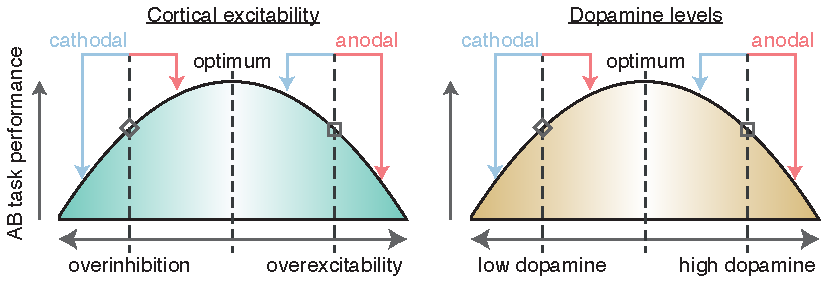
\includegraphics{AB_sEBR_files/figures/figure_1_model.pdf}
\caption{\label{fig:AB-sEBR-fig-model}\textbf{Model where AB task performance is dependent on cortical excitability \autocite[left,][]{London2015} and dopamine levels \autocite[right,][]{Wiegand2016}}. Whether anodal (red arrows) or cathodal (blue arrows) tDCS improves performance depends on the baseline starting point on these axes, as shown in two example cases. First, an individual with relatively low levels of dopamine / cortical excitability (diamond shape) should benefit from anodal tDCS (as they move closer to the optimum), whereas cathodal tDCS would be detrimental (as they are pushed further away from the optimum). Reversely, an individual with high levels of dopamine / cortical excitability (square shape) would benefit from cathodal but not anodal tDCS.}
\end{figure}



\hypertarget{AB_sEBR-methods}{%
\section{Materials and methods}\label{AB_sEBR-methods}}

A different set of results based on this dataset were reported in Chapter \ref{AB-tDCS-EEG}. We include the full materials and methods here for convenience.\footnote{Compared to Chapter \ref{AB-tDCS-EEG}, the \protect\hyperlink{AB_sEBR-participants}{Participants}, \protect\hyperlink{AB_sEBR-task}{Task}, and \protect\hyperlink{AB_sEBR-tDCS}{tDCS} sections are virtually identical; the \protect\hyperlink{AB_sEBR-procedure}{Procedure} section has been adapted to include the sEBR measurement, the \protect\hyperlink{AB_sEBR-stats}{Statistical analysis} and \protect\hyperlink{AB_sEBR-sEBR}{sEBR} sections are entirely novel.}

\hypertarget{AB_sEBR-participants}{%
\subsection{Participants}\label{AB_sEBR-participants}}

Fourty-eight participants took part in total, 8 of whom were excluded after the first session. One participant was excluded as a precaution because they developed an atypical headache after the first session, and we could not rule out this was related to the tDCS. Another stopped responding to our requests to schedule the second session. The remaining six participants were excluded because their mean T1 accuracy in the first session was too low, which would leave too few trials to analyze, because our T2 accuracy measure included only trials in which T1 was seen. We used a cut-off of 63\% T1 accuracy as an exclusion criterium, which was two standard deviations below the mean of a separate pilot study (n = 10).

This left a final sample of 40 participants (29 female, mean age = 20.94, \emph{SD} = 2.45, range = 18--28). This sample size was determined a priori to slightly exceed \textcite{London2015} (n = 34). Mean T1 accuracy in the remaining 40 participants was 82\%, which is comparable to previous studies using this task \autocites[86\% in][]{London2015}[in 82\% in][]{Slagter2013}.

The experiment and recruitment took place at the University of Amsterdam. All procedures for this study were approved by the ethics review board of the Faculty for Social and Behavioral Sciences, and complied with relevant laws and institutional guidelines. All participants provided their written informed consent and were compensated with course credit or €10 per hour (typically €65 for completing two full sessions).

\hypertarget{AB_sEBR-procedure}{%
\subsection{Procedure}\label{AB_sEBR-procedure}}

The study procedures were identical to \textcite{London2015}: participants received anodal and cathodal tDCS in separate sessions (Figure \ref{fig:AB-sEBR-fig-procedure}), which typically took place exactly one week apart (for 29 participants; sessions were separated by 6 days for 6 participants; 8 days for 3 participants; 4 days for 1 participant; 10 days for 1 participant). The time in between served to keep the sessions as similar as possible, and to minimize the risk of tDCS carry-over effects. 18 participants received anodal tDCS in the first session and cathodal tDCS in the second, and vice versa for the remaining 22 participants.

First, participants experienced the sensations induced by tDCS in a brief trial stimulation (see the \protect\hyperlink{AB_sEBR-tDCS}{tDCS} section). Next, sEBR was measured for 6 minutes (see the \protect\hyperlink{AB_sEBR-sEBR}{sEBR} section), after which participants completed 20 practice trials of the task (see the \protect\hyperlink{AB_sEBR-task}{Task} section). For the main portion of the experiment, participants performed three blocks of the task (Figure \ref{fig:AB-sEBR-fig-procedure}): before tDCS (\emph{baseline}), during anodal/cathodal tDCS (\emph{tDCS}), and after tDCS (\emph{post}).

Within each block of the task, participants took a self-timed break every 50 trials (\textasciitilde{}5 minutes); between the blocks, the experimenter walked in. Participants performed the task for exactly 20 minutes during the \emph{baseline} and \emph{post} blocks. During the \emph{tDCS} block, the task started after the 1-minute ramp-up of the current was complete, and continued for 21 minutes (constant current, plus 1-minute of ramp-down).

\begin{figure}
\centering
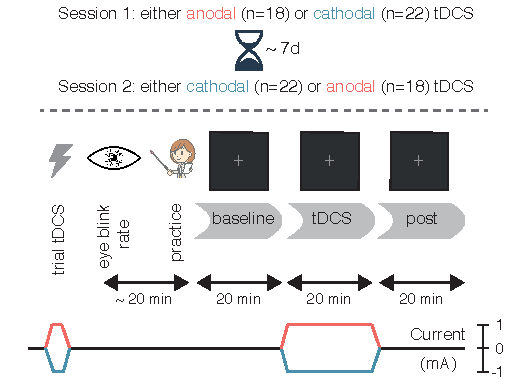
\includegraphics{AB_sEBR_files/figures/figure_2_procedure.pdf}
\caption{\label{fig:AB-sEBR-fig-procedure}\textbf{Experimental design}. Spontaneous eye blink rate was measured for 6 minutes prior to the start of the task. Then (following a short practice block), participants performed three 20-minute blocks of the attentional blink task: a \emph{baseline} block without stimulation, a \emph{tDCS} block during 20 minutes of anodal (red) or cathodal (blue) stimulation, and finally a \emph{post}-test block (also without stimulation). The second session (typically 7 days later at the same time of day) was identical, except that the tDCS polarity was reversed.}
\end{figure}



\hypertarget{AB_sEBR-task}{%
\subsection{Task}\label{AB_sEBR-task}}

The attentional blink task (Figure \ref{fig:AB-sEBR-fig-task}) was almost identical to the one used in \textcite{London2015} and \textcite{Slagter2013}, which in turn was based on a task designed by \textcite{Dux2008}. A rapid serial visual presentation stream of 15 letters (cf.~17 letters in \textcite{London2015}) was shown on each trial, using Presentation software (Neurobehavioral Systems, Inc.). Each letter was displayed for 91.7 ms (11 frames at 120 Hz) on a dark gray background. The letters were presented in font size 40 (font: Courier New) at a viewing distance of 90 cm. On each trial, the letters were randomly sampled without replacement from the alphabet, excluding the letters I, L, O, Q, U and V, as they were too similar to each other. All distractor letters were mid-gray, whereas T1 and T2 were colored. T1 was red and always appeared at position 5 in the stream. T2 was green and followed T1 after either 2 distractors (\emph{lag 3}) or 7 distractors (\emph{lag 8}) (cf.~lags 2, 4 and 10 in \textcite{London2015}).

The letter stream was preceded by a fixation cross (same color as the letters) presented for 1750 ms and followed by another fixation cross (presented for 1000 ms). Finally, the participant was prompted to type in (using a standard keyboard) the letter they thought was presented as T1 (``Which letter was red?''), followed by T2 (``Which letter was green?'').

Trial duration varied slightly because both the T1 and T2 response questions were self-paced, so some participants completed more trials than others depending on their response times. On average, participants completed 130 short lag trials (\emph{SD} = 17; range = 78--163) and 65 long lag trials (\emph{SD} = 9; range = 39--87) per 20-minute block.

\begin{figure}
\centering
\includegraphics{AB_sEBR_files/figures/figure_3_task.pdf}
\caption{\label{fig:AB-sEBR-fig-task}\textbf{Attentional blink task}. Participants viewed rapid serial visual presentation streams of 15 letters, all of which were distractors (gray letters) except for T1 and T2. T1 was presented in red at position 5; T2 was presented in green and followed T1 after 2 distractors (\emph{lag 3}, inside the AB window) or 7 distractors (\emph{lag 8}, outside the AB window). At the end of the trial, participants reported the identity of T1 and then T2 (self-paced).}
\end{figure}



\hypertarget{AB_sEBR-tDCS}{%
\subsection{tDCS}\label{AB_sEBR-tDCS}}

Transcranial direct current stimulation was delivered online (i.e.~during performance of the attentional blink task) using a DC-STIMULATOR PLUS (NeuroCare Group GmbH). The current was ramped up to 1 mA in 1 minute, stayed at 1 mA for 20 minutes, and was ramped down again in 1 minute.

One electrode was placed at F3 (international 10-20 system) to target the lDLPFC; the other was placed over the right forehead, centered above the eye (approximately corresponding to position Fp2). Both electrodes were 5 x 7 cm in size (35 cm\textsuperscript{2}), leading to a current density of 0.029 mA/cm\textsuperscript{2}. The electrode montage and tDCS parameters are identical to \textcite{London2015}, with two exceptions. First, we also measured EEG (see the \protect\hyperlink{AB_sEBR-sEBR}{sEBR} section), so the EEG electrodes and headcap were applied on top of the tDCS electrodes. Second, we used Ten20 paste (Weaver and Company) as the conductive medium, whereas \textcite{London2015} used sponges soaked in saline.

Participants received either anodal tDCS (anode on F3, cathode on right forehead) or cathodal tDCS (cathode on F3, anode on right forehead) in separate sessions. The procedure was double-blinded: both the participant and the experimenters were unaware which polarity was applied in a given session. The experimenter loaded a stimulation setting on the tDCS device (programmed by someone not involved in data collection), without knowing whether it was mapped to anodal or cathodal tDCS. In the second session, the experimenter loaded a second setting mapped to the opposite polarity (half the dataset), or simply connected the terminals of the device to the electrodes in the opposite way.

At the start of the experiment, participants received a brief trial stimulation, based on which they decided whether or not they wanted to continue with the rest of the session. The experimenter offered to terminate the experiment in case tDCS was experienced as too uncomfortable, but none of the participants opted to do so. For the trial stimulation, the current was ramped up to 1 mA in 45 seconds, stayed at 1 mA for 15 seconds, and was ramped down again in 45 seconds.

\hypertarget{AB_sEBR-sEBR}{%
\subsection{sEBR}\label{AB_sEBR-sEBR}}

Movement of the eyelids across the eyes affects the electrical potential that naturally exists across the eyeball \autocite{Matsuo1975}. Blinks can thus be recorded with electrodes placed on the face and/or scalp \autocite{Luck2005}.

We used a BioSemi ActiveTwo system with 64 Ag/AgCl active electrodes, placed according to the (10-10 subdivision of the) international 10-20 system. Two pairs of additional external electrodes were placed to record the electro-oculogram (EOG): above and below the left eye, and next to the left and right outer canthi. Finally, another pair of electrodes on the left and right earlobes served as the reference. This full setup was used because we also recorded the EEG during task performance. This dataset is available elsewhere \autocite{Reteig2019_data}.

sEBR was recorded for 6 minutes after setting up the EEG in each session. Participants were asked to sit still and look straight ahead at a white wall (about 1 meter away). Participants were told they were allowed to move their eyes, but the experimenter made no mention of eye blinks. The ``cover story'' was that we needed to monitor the quality of the EEG signal before being able to start the recordings. Because blink rate can increase in the evening \autocite{Barbato2000}, but is stable during the day time \autocites{Barbato2000}{Doughty2006}, we made sure all recordings were completed before 5 PM. Most participants started their first and second sessions at the exact same time of day (34 participants; 4 participants started their second session 5 hours earlier/later than their first, 2 started 3 hours earlier/later).

The raw data were preprocessed using the EEGLAB toolbox \autocite{Delorme2004} in MATLAB (MathWorks, Inc.). First, data were re-referenced offline to the average of the earlobe electrodes. Next, horizontal and vertical EOG channels were created by subtracting the signals from each member of a horizontal/vertical electrode pair. A high-pass filter with a cut-off of .5 Hz was then applied. Finally, we ran an independent component analysis (ICA) to capture the eye blink events in a single time series. For each recording, we visually inspected the independent components and selected one that appeared to contain the eye blink signals, based on the waveform (large amplitude, positive deflections) and scalp distribution of the ICA weights (loading on frontal and EOG electrodes).

Eye blinks in this component were then detected using a semi-automatic procedure \autocites[cf.][]{Slagter2013}{Kruis2016}. First, a voltage threshold was set (initialized to the standard deviation of the signal) which captured most eye blink peaks. This threshold was moved up or down by the analyst if necessary. The sample with the maximum voltage between two threshold crossings was marked as an eye blink, with the restriction that two eye blinks must be at least 400 ms apart. We picked 400 ms as an upper estimate of the duration of a single blink \autocite{Caffier2003}. The analyst then inspected the output, and removed or added eye blinks in the case of clear false positives (e.g., a muscle contraction) or false negatives (e.g., an eye blink waveform did not exceed the threshold, or was followed by another clear eye blink within 400 ms).

\hypertarget{AB_sEBR-stats}{%
\subsection{Statistical analysis}\label{AB_sEBR-stats}}

Data were analyzed using R \autocite[Version 3.5.1;][]{R-base}\footnote{We, furthermore, used the R-packages \emph{broom} \autocite[Version 0.5.1;][]{R-broom}, \emph{cowplot} \autocite[Version 0.9.99;][]{R-cowplot}, \emph{here} \autocite[Version 0.1;][]{R-here}, \emph{knitr} \autocite[Version 1.21;][]{R-knitr}, \emph{lubridate} \autocite[Version 1.7.4;][]{R-lubridate}, \emph{papaja} \autocite[Version 0.1.0.9842;][]{R-papaja}, and \emph{tidyverse} \autocite[Version 1.2.1;][]{R-tidyverse}.} from within RStudio \autocite[Version 1.1.463;][]{RStudio2016}. Our analyses were focused on three dependent variables. \emph{sEBR} was expressed as the number of eye blinks per minute. For the AB, we examined T2\textbar{}T1 accuracy, i.e.~the percentage of trials where T2 was reported correctly, out of the subset of trials in which T1 was reported correctly. The size of the attentional blink (\emph{AB magnitude}) was quantified by subtracting T2\textbar{}T1 accuracy at lag 3 from T2\textbar{}T1 accuracy at lag 8, for each session in each block. Lastly, we created \emph{AB magnitude change scores} for each session by subtracting AB magnitude in the ``baseline'' block from the ``tDCS'' and the ``post'' blocks, respectively.

\hypertarget{AB_sEBR-methods-rel}{%
\subsubsection{Reliability}\label{AB_sEBR-methods-rel}}

We evaluated the test-retest reliability of sEBR and AB magnitude across sessions by computing intraclass correlations (ICCs) using the \emph{psych} package \autocite[Version NA;][]{R-psych}. We primarily report the single-rating, two-way ICC for absolute agreement, also known as ICC(2,1) in the conventions from \textcite{Shrout1979}. This is the most appropriate ICC for test-retest reliability \autocite{Koo2016}. In addition, we report Pearson's correlation, to be able to compare the reliability of sEBR with \textcite{Dang2017}, and ICC(3,2), also known as Cronbach's alpha \autocite{McGraw1996}, to compare our results with \textcite{Kruis2016}. We used the interpretation scheme in \textcite{Koo2016}, which classifies reliability as ``poor'' for ICCs \textless{} .5, .5 \textless{} ICC \textless{} .75 as ``moderate'', .75 \textless{} ICC \textless{} .9 as ``good'', and ICCs \textgreater{} .9 as ``excellent''. For AB magnitude, we also report Pearson's correlation, as this measure was used by all previous studies on the reliability of the AB \autocite[e.g.][]{Dale2013}. Here we also used data from the \emph{baseline} block only, to rule out any influence of tDCS on the reliability scores.

\hypertarget{AB_sEBR-methods-base}{%
\subsubsection{Relation between sEBR and baseline AB magnitude}\label{AB_sEBR-methods-base}}

\hypertarget{linear-relationships}{%
\paragraph{Linear relationships}\label{linear-relationships}}

We calculated Pearson correlations to test for linear relationships between \emph{sEBR} and \emph{AB magnitude}. We also computed a Bayes factor for these correlations, as proposed by \textcite{Ly2016} and implemented in the \emph{BayesFactor} package \autocite[Version NA;][]{R-BayesFactor}, with the standard prior distribution (\(\kappa\) = .33). This Bayes factor (\(BF_{01}\)) expresses the relative evidence for the null hypothesis of zero correlation, vs.~the alternative hypothesis that there is a non-zero correlation. We use the interpretation scheme from \textcite{Wagenmakers2018}, where \(1 < BF_{01} < 3\) constitutes ``anecdotal'' evidence for the null, \(3 < BF_{01} < 10\) \textasciitilde{} ``moderate'' evidence, and \(10 < BF_{01} < 30\) \textasciitilde{} ``strong'' evidence.

Because \textcite{Colzato2008} previously reported a negative relationship between \emph{sEBR} and \emph{AB magnitude}, we computed two additional Bayes Factors that incorporate this prior information. First, we used the same prior but folded all of its mass to negative effect sizes only, effectively providing a Bayes factor for a one-sided test \autocite{Wagenmakers2016}. This Bayes factor (\(BF_{0-}\)) expresses the relative evidence for the null hypothesis of zero correlation, vs.~the alternative hypothesis that there is a negative correlation. Second, we computed a replication Bayes Factor, by using the posterior from \textcite{Colzato2008} as a prior \autocites{Verhagen2014}{Wagenmakers2016}. This Bayes factor (\(BF_{0r}\)) expresses the relative evidence for the null hypothesis of zero correlation, vs.~the alternative hypothesis that the correlation is as in \textcite{Colzato2008}.

\hypertarget{inverted-u-shaped-relationships}{%
\paragraph{Inverted-U-shaped relationships}\label{inverted-u-shaped-relationships}}

To evaluate the presence of an (Inverted-) U-shaped relationship between \emph{sEBR} and \emph{AB magnitude}, we used the ``two-lines test'' as proposed by \textcite{Simonsohn2018}. This test revolves around the core assumption in any U-shaped relationship: that a sign flip occurs at a break point in the data. Values on one side of this break point should exhibit a positive relationship (rising flank of the U); values on the other side should exhibit a negative relationship (falling flank of the U). The ``two-lines test'' first estimates the value of the break point based on a cubic spline fit to all of the data, and then computes two linear regressions to estimate the slopes on either side of the break point. Both slopes have to be significant and of opposite sign to reject the null hypothesis that there is no U-shaped relationship.

\hypertarget{relation-between-sebr-and-the-effect-of-tdcs-on-ab-magnitude}{%
\subsubsection{Relation between sEBR and the effect of tDCS on AB magnitude}\label{relation-between-sebr-and-the-effect-of-tdcs-on-ab-magnitude}}

We also calculated Pearson and Bayesian correlations between sEBR and \emph{AB magnitude change scores}, cf.~the relation between sEBR and AB magnitude at baseline. In general, such a correlation \(r_{A(Y-X)}\) between a change score \(Y-X\) (here, AB magnitude in the \emph{tDCS} or \emph{post} block minus the \emph{baseline} score) and another variable \(A\) (here, sEBR), is a function of four components: 1) \(r_{AX}\): the correlation between \(A\) and the pre-test \(X\), 2) \(r_{AY}\): the correlation between \(A\) and the post-test \(Y\), 3) \(r_{XY}\): the correlation between pre- and post-test (i.e., the reliability), and 4) \(SD_y / SD_x\): the ratio between the standard deviations of the pre- and post-test \autocites{Gardner1987}{Griffin1999}. Next to the correlation with the difference score, we also computed these constituent components (reported in Tables \ref{tab:ABmag} and \ref{tab:corrco}). A complementary way to test for \(r_{A(Y-X)}\) is to test whether \(r_X\) and \(r_Y\) are significantly different. We used the Pearson-Filon test \autocite*{Pearson1898} for this purpose, as implemented in the \emph{cocor} package \autocite[Version NA;][]{R-cocor}.

\hypertarget{data-materials-and-code-availability-2}{%
\subsection{Data, materials, and code availability}\label{data-materials-and-code-availability-2}}

All of the data, materials, and code for this study are available on the \href{https://doi.org/10.17605/OSF.IO/PZBGY}{Open Science Framework}. The raw task data and sEBR recordings can also be downloaded from this page. The code to preprocess the sEBR data and perform the semi-automatic eye blink detection \autocites[cf.][]{Slagter2013}{Kruis2016} is supplied in MATLAB scripts. We provide the statistical analysis code in the form of an R notebook, detailing all the analyses that we ran for this project, along with the results. We also include an Rmarkdown \autocite{Xie2018} source file for this paper that can be run to reproduce the pdf version of the text, along with all the figures and statistics.

\hypertarget{AB_sEBR-results}{%
\section{Results}\label{AB_sEBR-results}}

\hypertarget{AB_sEBR-results-rel}{%
\subsection{Reliability}\label{AB_sEBR-results-rel}}

We first examined task performance in the baseline block of both sessions, i.e.~before tDCS onset. All participants showed the characteristic AB effect in both sessions: T2\textbar{}T1 accuracy was higher for lag 8 trials than for lag 3 (Figure \ref{fig:fig-retest}A).

There was also a significant difference in AB magnitude (lag 8 minus lag 3 T2\textbar{}T1 accuracy) between the sessions: (\emph{F}(1, 39) = 16.53, \emph{p} \textless{} .001). For most participants, AB magnitude was smaller in the second session than the first (Figure \ref{fig:fig-retest}B). The average difference in AB magnitude over sessions seemed to be driven by lag 3 performance only (Figure \ref{fig:fig-retest}A), meaning the AB genuinely decreased with practice.

To be able to uncover relationships between sEBR and AB magnitude (see the \protect\hyperlink{AB_sEBR-ABmag}{subsequent sections}), it is crucial that the test-retest reliability of both measures is adequate, i.e.~that there is substantial agreement between the scores in session 1 and 2.

The intraclass correlation for AB magnitude (Figure \ref{fig:fig-retest}B) is .60, indicating ``moderate'' test-retest reliability \autocite{Koo2016}, with a 95\% confidence interval of .25 (poor) -- .79 (good). The standard (interclass) Pearson correlation for AB magnitude between sessions is comparable (\emph{r}(38) = .68, CI\textsubscript{95\%} {[}.47, .82{]}) and comparable to previous reports \autocite{Dale2013}.

In contrast to AB magnitude, sEBR (Figure \ref{fig:fig-retest}C), did not differ significantly between sessions (\emph{F}(1, 39) = 0.149, \emph{p} = 0.701). We had some concerns that participants would blink less in the second session, because they had been instructed (after the sEBR measurement in session 1) that blinking can cause artifacts in the EEG signal (recorded during task performance). Yet, if anything, median sEBR was slightly higher in the second session (12.6) than the first (11.7). However, we also asked participants whether they had been in an EEG experiment

\newpage
\pagestyle{empty}
\changetext{}{}{-25mm}{}{}
\blandscape
\captionsetup{width=\linewidth}

\begin{figure}
\includegraphics[width=180mm]{AB_sEBR_files/figures/figure_4_retest} \caption{\textbf{Reliability of the attentional blink and spontaneous eye blink rate}. (\textbf{A}) All participants showed an attentional blink in both sessions: higher T2\textbar{}T1 accuracy (\% T2 correct in trials where T1 was also correct) for lag 8 (orange) than lag 3 (yellow). Horizontal lines show group-average T2\textbar{}T1 accuracy. The attentional blink magnitude (lag 8 - lag 3) is slightly smaller in the second session (dotted lines) than the first session (solid lines), due to better lag 3 performance on average. (\textbf{B}) AB magnitude for each participant in session 1 vs.~2. The intraclass correlation indicates moderate test-retest reliability, though the 95\% confidence interval ranges all the way from poor to good. AB magnitude in (\textbf{A}) and (\textbf{B}) was calculated on the \emph{baseline} block only, before tDCS onset. (\textbf{C}) sEBR values for each participant in session 1 vs.~2. The intraclass correlation indicates that the test-retest reliability for sEBR is good.}\label{fig:fig-retest}
\end{figure}



\newpage
\elandscape
\changetext{}{}{+25mm}{}{}
\pagestyle{\defstyle}
\captionsetup{width=\textwidth}

\noindent before. Participants that had done so exhibited a greatly reduced median sEBR in both sessions (6.3 in session 1; 4.1 in session 2). Because these were only 6 cases in an already small sample, we are unsure whether this finding is robust, but it is a cautionary note to others aiming to measure sEBR using (a full setup of) EEG electrodes. Because smoking has been reported to increase sEBR \autocite{Klein1993}, we also asked whether participants self-identified as a smoker (n = 5). These individuals were not clear outliers in the distribution, neither were those wearing contact lenses (n = 4), which also generally should increase blink rate.

Most importantly, the test-retest reliability for sEBR was ``good'' \autocite{Koo2016}, indicated by an intraclass correlation of .85 CI\textsubscript{95\%} {[}.73, .92{]}. The Pearson correlation was \emph{r}(38) = .84, CI\textsubscript{95\%} {[}.72, .91{]} \autocite[cf.][]{Dang2017}; Cronbach's alpha was .91, CI\textsubscript{95\%} {[}.84, .95{]} \autocite[cf.][]{Kruis2016}.

One participant's sEBR in session 2 seems remarkably high (57 blinks per minute), and is quite a bit higher in session 2 than in session 1 (difference of 12). However, we confirmed this was not a data quality issue, and rerunning the analyses without this participant did not qualitatively change the results in the subsequent sections. Hence, this participant was included in all analyses.

\hypertarget{AB_sEBR-ABmag}{%
\subsection{Relation between sEBR and baseline AB magnitude}\label{AB_sEBR-ABmag}}

\begin{figure}
\centering
\includegraphics{AB_sEBR_files/figures/figure_5_AB-corr.pdf}
\caption{\label{fig:fig-AB-corr}\textbf{No significant relationships between sEBR and AB magnitude in the block before tDCS onset}. Grey solid lines show a linear fit over all data points (individual participants), with no clear relationship in both sessions. Grey dashed lines show a cubic spline fit over all data points. Colored lines show two separate linear fits, delimited by the break point in the cubic spline, as estimated with the ``two-lines test'' \autocite{Simonsohn2018}. Both the spline fit and the two linear slopes suggest an Inverted-U shaped relationship in session 1, but neither slope is significant, and this pattern is not present in session 2.}
\end{figure}



Based on the results of \textcite{Colzato2008}, we should expect to find a negative correlation between sEBR and AB magnitude (in the baseline block). However, the correlation here was not significant in either session 1 (\emph{r}(38) = .08, CI\textsubscript{95\%} {[}-.24, .38{]}, \emph{p} = .637), or session 2 (\emph{r}(38) = .003, CI\textsubscript{95\%} {[}-.31, .31{]}, \emph{p} = .987). The direction of the effect is close to zero or slightly positive (Figure \ref{fig:fig-AB-corr}), which is not in accord with \textcite{Colzato2008}.

Bayesian correlations show that the data are BF\textsubscript{01} = 2.57 times (session 1) and BF\textsubscript{01} = 2.84 times (session 2) more likely under the null hypothesis, using the default prior. This constitutes some evidence for absence of a correlation, though not more than anecdotal. If we evaluate the prior over negative effect sizes only \autocite[based on the negative correlation in][]{Colzato2008}, the support for the null increases slightly and becomes moderate (session 1: BF\textsubscript{0-} = 3.90, session 2: BF\textsubscript{0-} = 2.87). Finally, if we use the correlation as in \textcite{Colzato2008} (\emph{r}(18) = -.53) as a prior \autocite{Wagenmakers2016}, the support for the null hypothesis becomes strong (session 1: BF\textsubscript{0r} = 15.80, session 2: BF\textsubscript{0r} = 10.43).

We also probed for an Inverted-U-shaped relationship between sEBR and AB magnitude, using the ``two lines test'' \autocite{Simonsohn2018}. In session 1, a cubic spline-fit indeed suggests an Inverted-U-shaped relationship (Figure \ref{fig:fig-AB-corr}). The linear regressions do as well, since the first slope is positive (\emph{b} = .012, \emph{p} = .058) and the second is negative (\emph{b} = -.006, \emph{p} = .602). However, neither slope is significant. Furthermore, this pattern is absent in session 2 (line 1: \emph{b} = .001, \emph{p} = .931; line 2: \emph{b} = .003, \emph{p} = .545), with the spline fit also showing a more erratic pattern.

\hypertarget{relation-between-sebr-and-the-effect-of-tdcs-on-ab-magnitude-1}{%
\subsection{Relation between sEBR and the effect of tDCS on AB magnitude}\label{relation-between-sebr-and-the-effect-of-tdcs-on-ab-magnitude-1}}

\begin{figure}
\includegraphics[width=130mm]{AB_sEBR_files/figures/figure_6_tDCS-corr} \caption{\textbf{No significant relationships between sEBR and AB magnitude change scores.} Each plot shows spontaneous eye blink rates on the x-axis, and the change in AB magnitude on the y-axis (difference scores of the \emph{tDCS} block - the \emph{baseline} block, or the \emph{post} block - \emph{baseline}) in the \emph{anodal} and \emph{cathodal} stimulation conditions.}\label{fig:fig-tDCS-corr}
\end{figure}



Although there was no relationship between sEBR and AB magnitude itself, sEBR could potentially still be associated with tDCS-induced changes in AB magnitude. We therefore computed AB magnitude change scores (\emph{tDCS - baseline}, \emph{post - baseline}) in each stimulation condition (\emph{anodal}, \emph{cathodal}), and correlated these to sEBR. However, this analysis did not uncover any significant relationships (Figure \ref{fig:fig-tDCS-corr} and columns 2--4 in Table \ref{tab:corrco}). These change score correlations are ultimately based on a number of different variables: the within-session reliability of AB magnitude (Table \ref{tab:ABmag}), the within-block variability in AB magnitude (Table \ref{tab:corrco}), and, most importantly, the separate correlations between sEBR and AB magnitude in each block (Table \ref{tab:ABmag}). None of the correlations in the baseline block differed significantly from the correlations in the subsequent blocks (columns 5--6 in Table \ref{tab:corrco}), again suggesting there was no relationship between sEBR and AB magnitude change scores.

\begin{table}

\caption{\label{tab:ABmag}Variability of attentional blink magnitude scores and correlation with sEBR, per stimulation condition and block.}
\centering
\fontsize{10}{12}\selectfont
\begin{threeparttable}
\begin{tabular}[t]{>{\raggedright\arraybackslash}p{10em}rr}
\toprule
Block & $r$ sEBR\textsuperscript{a} & SD\textsuperscript{b}\\
\midrule
\addlinespace[0.3em]
\multicolumn{3}{l}{\textbf{anodal session}}\\
\hspace{1em}baseline & .04 & 0.140\\
\hspace{1em}tDCS & .15 & 0.148\\
\hspace{1em}post & .25 & 0.137\\
\addlinespace[0.3em]
\multicolumn{3}{l}{\textbf{cathodal session}}\\
\hspace{1em}baseline & .05 & 0.136\\
\hspace{1em}tDCS & -.05 & 0.128\\
\hspace{1em}post & .09 & 0.120\\
\bottomrule
\end{tabular}
\begin{tablenotes}
\item[a] Pearson's correlation between AB magnitude and spontaneous eye blink rate
\item[b] Standard deviation of AB magnitude
\end{tablenotes}
\end{threeparttable}
\end{table}

\begingroup

\begin{table}

\caption{\label{tab:corrco}Attentional blink magnitude and spontaneous eye blink rate correlations.}
\centering
\fontsize{10}{12}\selectfont
\begin{threeparttable}
\begin{tabular}[t]{lrrrrrr}
\toprule
\multicolumn{1}{c}{ } & \multicolumn{3}{c}{Correlation\textsuperscript{a}} & \multicolumn{2}{c}{\makecell[c]{Pearson-Filon\\test\textsuperscript{b}}} & \multicolumn{1}{c}{Reliability\textsuperscript{c}} \\
\cmidrule(l{3pt}r{3pt}){2-4} \cmidrule(l{3pt}r{3pt}){5-6} \cmidrule(l{3pt}r{3pt}){7-7}
contrast & $r$ & $p$ & $BF_{01}$ & $Z$ & $p$ & $r$\\
\midrule
\addlinespace[0.3em]
\multicolumn{7}{l}{\textbf{anodal session}}\\
\hspace{1em}tDCS - baseline & .21 & .199 & 1.37 & -1.27 & .204 & .84\\
\hspace{1em}post - baseline & .24 & .133 & 1.05 & -1.59 & .111 & .63\\
\addlinespace[0.3em]
\multicolumn{7}{l}{\textbf{cathodal session}}\\
\hspace{1em}tDCS - baseline & -.16 & .313 & 1.81 & 1.05 & .296 & .82\\
\hspace{1em}post - baseline & .04 & .808 & 2.77 & -0.33 & .745 & .71\\
\bottomrule
\end{tabular}
\begin{tablenotes}
\item[a] Linear correlation (Pearson and Bayesian) between sEBR and AB magnitude change scores
\item[b] Test for significant differences between the sEBR vs. AB magnitude correlations (reported in Table \ref{tab:ABmag}) in the baseline vs. tDCS or post blocks
\item[c] Pearson correlation between AB magnitude scores in the baseline vs. tDCS or post blocks
\end{tablenotes}
\end{threeparttable}
\end{table}

\endgroup

\hypertarget{AB_sEBR-discussion}{%
\section{Discussion}\label{AB_sEBR-discussion}}

Dopamine levels play a central role in regulating cognitive functions. tDCS may be used to enhance cognitive functions, but its precise effects appear to be dependent on dopamine as well. Here we attempted to use sEBR---a proxy for dopaminergic activity---to study how dopamine may determine the size of the AB and its modulation by tDCS. As a prerequisite, we assessed the test-retest reliabilities of sEBR and AB magnitude, which proved to be good to moderate, respectively, in line with previous reports \autocites{Kruis2016}{Dang2017}{Dale2013}. We then attempted to replicate a result from \textcite{Colzato2008}, who reported that individuals with high sEBR tend to exhibit a smaller AB. However, we found no significant linear or Inverted-U-shaped relationship between sEBR and AB magnitude, with more evidence for the null hypothesis of no association. Finally, we also did not find any evidence that sEBR is associated with the effects of tDCS on AB magnitude.

\hypertarget{sebr-and-ab-magnitude-have-good-to-moderate-test-retest-reliability}{%
\subsection{sEBR and AB magnitude have good to moderate test-retest reliability}\label{sebr-and-ab-magnitude-have-good-to-moderate-test-retest-reliability}}

The test-retest reliability of sEBR across two testing sessions (separated by about one week) was ``good'', bordering on ``excellent'' \autocite{Koo2016}. Only two other studies examined the reliability of sEBR to date. \textcite{Dang2017} (n = 18) found a Pearson correlation of .86 between sEBR under administration of bromocriptine (a dopamine agonist) or placebo (separated by 4 hours). Here, Pearson's correlation was comparable (.84). In \textcite{Kruis2016}, Cronbach's alpha for sEBR ranged from .85 (three measurements of 27 long-term meditators) to .79 (2--3 measurements of 114 meditation-naive participants). In our data, Cronbach's alpha was even slightly higher (.91). Together, all three studies suggest that sEBR scores are trait-like and stable over time, even for short measurements of only several minutes (6 minutes here and in \textcite{Kruis2016}; 5 minutes in \textcite{Dang2017}). Although the reliability estimates are comparable, we measured sEBR twice under baseline conditions, whereas \textcite{Dang2017} administered a dopamine agonist in one measurement (vs.~placebo), and \textcite{Kruis2016} measured sEBR following meditation practice (vs.~a regular day). We did find that participants with prior EEG experience exhibited a two- to threefold lower sEBR. Future studies that measure sEBR with EEG electrodes might want to take this into account. However, this observation was based on only 6 participants, and sEBR did not significantly differ between sessions, despite the fact that all participants had EEG experience after the first session.

In contrast to sEBR, AB magnitude was significantly smaller in the second session. Previous studies have reported that performance on an AB task can improve across sessions \autocites{Dale2013}{Slagter2007}, but for targets at all lags, whereas here we observed a specific increase in lag 3 T2\textbar{}T1 performance (inside the attentional blink window). Test-retest reliability of AB magnitude was lower than sEBR: the point-estimate indicated only ``moderate'' reliability, though the 95\% confidence interval was also consistent with ``poor'' to ``good'' reliability. However, this is comparable to previous reports (see Table \ref{tab:AB-reliability}). The Pearson correlation in the present study (\emph{r} = .68) is even on the higher end of the range reported in previous studies (though note that regular correlations can overestimate ``true'' test-retest reliability \autocite{Bland1986}).

\begingroup
\small

\LTcapwidth=\textwidth

\begin{longtable}[]{@{}llll@{}}
\caption{\label{tab:AB-reliability} Previous reports on the reliability of AB magnitude. Note that these all used interclass (Pearson) correlations.}\tabularnewline
\toprule
\begin{minipage}[b]{0.19\columnwidth}\raggedright
Study\strut
\end{minipage} & \begin{minipage}[b]{0.03\columnwidth}\raggedright
n\strut
\end{minipage} & \begin{minipage}[b]{0.15\columnwidth}\raggedright
Correlation\strut
\end{minipage} & \begin{minipage}[b]{0.51\columnwidth}\raggedright
Notes\strut
\end{minipage}\tabularnewline
\midrule
\endfirsthead
\toprule
\begin{minipage}[b]{0.19\columnwidth}\raggedright
Study\strut
\end{minipage} & \begin{minipage}[b]{0.03\columnwidth}\raggedright
n\strut
\end{minipage} & \begin{minipage}[b]{0.15\columnwidth}\raggedright
Correlation\strut
\end{minipage} & \begin{minipage}[b]{0.51\columnwidth}\raggedright
Notes\strut
\end{minipage}\tabularnewline
\midrule
\endhead
\begin{minipage}[t]{0.19\columnwidth}\raggedright
\textcite{Kelly2011}\strut
\end{minipage} & \begin{minipage}[t]{0.03\columnwidth}\raggedright
37\strut
\end{minipage} & \begin{minipage}[t]{0.15\columnwidth}\raggedright
.33, .34, .48, .52,\strut
\end{minipage} & \begin{minipage}[t]{0.51\columnwidth}\raggedright
test and retest on same day; different values correspond to different tasks\strut
\end{minipage}\tabularnewline
\begin{minipage}[t]{0.19\columnwidth}\raggedright
\textcite{Dale2013a}\strut
\end{minipage} & \begin{minipage}[t]{0.03\columnwidth}\raggedright
46\strut
\end{minipage} & \begin{minipage}[t]{0.15\columnwidth}\raggedright
.62, .39\strut
\end{minipage} & \begin{minipage}[t]{0.51\columnwidth}\raggedright
test and retest one week apart; 1st value is a task with a set-switch, 2nd is without\strut
\end{minipage}\tabularnewline
\begin{minipage}[t]{0.19\columnwidth}\raggedright
\textcite{Dale2013}\strut
\end{minipage} & \begin{minipage}[t]{0.03\columnwidth}\raggedright
118\strut
\end{minipage} & \begin{minipage}[t]{0.15\columnwidth}\raggedright
.41, .41, .45, .48, .49\strut
\end{minipage} & \begin{minipage}[t]{0.51\columnwidth}\raggedright
test and retest one week apart; different values correspond to different tasks\strut
\end{minipage}\tabularnewline
\begin{minipage}[t]{0.19\columnwidth}\raggedright
\textcite{London2015}\strut
\end{minipage} & \begin{minipage}[t]{0.03\columnwidth}\raggedright
34\strut
\end{minipage} & \begin{minipage}[t]{0.15\columnwidth}\raggedright
.58\strut
\end{minipage} & \begin{minipage}[t]{0.51\columnwidth}\raggedright
test and retest one week apart; almost same task as present study\strut
\end{minipage}\tabularnewline
\bottomrule
\end{longtable}

\endgroup

The moderate reliability for AB magnitude limits the correlation that can be obtained between AB magnitude and sEBR. The AB phenomenon might suffer from the ``individual differences paradox'' \autocite{Hedge2018}: precisely because it is robust at the group level (almost everyone has an AB), it might not exhibit sufficient between-subject variability to be reliable. On the other hand, the AB seems to have a larger range of individual differences than other tasks \autocite{Willems2016}, and even a moderate reliability should provide ``enough room'' to detect correlations between sEBR and AB magnitude in a plausible range.

\hypertarget{no-significant-relationships-between-sebr-and-baseline-ab-magnitude}{%
\subsection{No significant relationships between sEBR and baseline AB magnitude}\label{no-significant-relationships-between-sebr-and-baseline-ab-magnitude}}

\textcite{Colzato2008} (n = 20) found a negative correlation between sEBR and AB magnitude. Here, this correlation was not significant in either session, with an effect size around 0 (session 2) or even slightly positive (session 1). The main difference between both studies seems to be the distribution of AB magnitude scores. The AB was shallow in \textcite{Colzato2008}, as average AB magnitude was less than 10\%, with 5 out of 20 participants showing either a ``negative'' AB (higher T2\textbar{}T1 accuracy at the shortest lag) or an AB magnitude around 0. Here, the blink was much more pronounced (40\% on average)---even the best performing participant had an AB magnitude (11\%) that exceeded the average in \textcite{Colzato2008}.

Our AB task also involves an attentional set switch, while the task used by \textcite{Colzato2008} did not. In our task, T1 and T2 had different features (T1 was red; T2 was green), so participants had to update their attentional template and detect the second target on the basis of a different feature (color) than T1. In \textcite{Colzato2008}, T1 and T2 were both digits, and thus belonged to the same set. \textcite{Kelly2011} suggest that such a set switch introduces an additional bottle neck that is dissociable from the AB \autocite{Potter1998}. However, follow-up studies have shown that there is still a sizable correlation between non-switch and switch-versions of AB tasks \autocites{Dale2013}{Dale2013a}. Although a set switch may introduce additional variance, it seems unlikely this would be sufficient to completely abolish a correlation between sEBR and AB magnitude. However, it could have reduced the size of the effect to a degree where it could no longer be reliably detected. The correlation between sEBR and AB magnitude in \textcite{Colzato2008} (\emph{r} = -.53) appears to exceed the average reliability of AB magnitude itself (Table \ref{tab:AB-reliability}), suggesting it might be an overestimate of the true correlation. Further evidence that the effect might be small comes from \textcite{Unsworth2019}, who conducted a large-scale study (n = 204) and only found a correlation of .17 between sEBR and attentional control (psychomotor vigilance task, antisaccade task), and no correlation with working memory (operation, symmetry, and reading span)---a core component in the AB \autocites{Dux2009}{Martens2010}. Although our sample size is twice that of \textcite{Colzato2008}, an effect of this magnitude would not have been detectable. It should also be noted that we used almost the same task as \textcite{Slagter2013} (n = 39), who also did not find a significant correlation between sEBR and AB magnitude. So both our studies do not support a relationship between sEBR and the AB.

No study to date has investigated an Inverted-U-shaped relationship between sEBR and AB magnitude, even though the underlying theory strongly suggests it \autocites{Cools2011}{Slagter2012}. Here the data do conform to a weak Inverted-U-shaped relationship, but only in session 1, and neither the upward nor the downward slope were significantly different from 0. Because both would have to be significant \autocite{Simonsohn2018}, and each slope is estimated on a different subset of the sample, we likely did not have sufficient power to detect an Inverted-U-shaped relationship. To be able to detect an Inverted-U-shaped relationship, the participants in our sample should also cover the whole range of AB task performance and dopamine levels. If this assumption is not met, then a true Inverted-U-shaped relationship could also masquerade as a linear effect (if all participants are sub-optimal), or no effect (if all participants are in the optimal range).

Two recent studies have cast doubt on the validity of sEBR as proxy for striatal dopamine. Both used PET to measure dopamine non-invasively in humans, but found no relation between sEBR and striatal dopamine receptor availability \autocite{Dang2017} or dopamine synthesis capacity \autocite{Sescousse2018}. So, even though we find no relation between sEBR and the AB, there could still be a true relationship between dopamine and the AB---sEBR might simply not have high validity to measure it accurately.

\hypertarget{no-significant-relationship-between-sebr-and-the-effect-of-tdcs-on-ab-magnitude}{%
\subsection{No significant relationship between sEBR and the effect of tDCS on AB magnitude}\label{no-significant-relationship-between-sebr-and-the-effect-of-tdcs-on-ab-magnitude}}

We suggested two factors that might underlie individual differences in the effects of tDCS on the AB (See Figure \ref{fig:AB-sEBR-fig-model}). First, baseline cortical excitability might partially determine whether tDCS leads to behavioral improvements or impairments \autocite{Krause2013} (Figure \ref{fig:AB-sEBR-fig-model}, left panel). This seems to fit the results of \textcite{London2015}, who found that individuals that benefited from anodal tDCS tended to worsen with cathodal tDCS (and vice versa). However, we did not replicate this negative correlation between the effects of anodal and cathodal tDCS (see Chapter \ref{AB-tDCS-EEG}), so this finding may not be robust.

Second, baseline dopamine levels may also partially determine the behavioral effects of tDCS \autocite{Wiegand2016} (Figure \ref{fig:AB-sEBR-fig-model}, right panel). Assuming that sEBR is a valid index of dopamine levels, we found no evidence for this result, though our Bayes Factor analyses also did not indicate strong evidence of absence. The model proposed by \textcite{Wiegand2016} is based on just two studies \autocites{Plewnia2013}{Nieratschker2015} that show different effects of tDCS in different COMT-subtypes, who should vary in baseline dopamine levels. However, a more recent study found that offline effects of prefrontal tDCS on working memory did not interact with COMT genotype \autocite{Jongkees2018}. Because tDCS may also induce activation of \autocite{Meyer2019} and dopamine release in the striatum \autocites{Tanaka2013}{Fonteneau2018}, the model is complicated even further. On a more basic level, it is also still disputed whether the COMT polymorphism can affect cognitive functioning \autocite{Barnett2008}, as most studies are likely severely underpowered \autocite{Border2019}. The only study that looked at the relation between COMT and the AB also found no association \autocite{Colzato2011}, although this was a very small study for genotyping standards. Thus, the overall evidence that the effect of tDCS on the AB depends on baseline dopamine levels is preliminary.

Finally, it is unclear how both axes of the model (Figure \ref{fig:AB-sEBR-fig-model}) relate to each other. Pairing tDCS with dopaminergic drugs produces complex and non-linear effects on cortical excitability \autocites{Monte-Silva2009}{Fresnoza2014}. Two studies that have combined tDCS and administration of tyrosine (a dopamine precursor) in cognitive tasks have indeed led to divergent results. Cathodal tDCS of the lDLPFC appears to counteract the beneficial effects of tyrosine, as their combination had no net behavioral effect \autocites{Jongkees2017}{Dennison2018}. In contrast, combining anodal tDCS with tyrosine led to impaired performance on an n-back task, where anodal tDCS alone would be expected to enhance performance \autocite{Jongkees2017}. Future studies that manipulate both dopamine levels and cortical excitability are necessary to uncover the physiology that could lead to such interactions.

\hypertarget{conclusions}{%
\subsection{Conclusions}\label{conclusions}}

We found that spontaneous eye blink rate is a reliable measure, but that it does not relate to the attentional blink, or to changes in attentional blink size following tDCS. Because dopamine is central to healthy cognitive and brain function, it remains plausible that dopamine interacts with manipulations of brain function, such as tDCS, as well as cognitive tasks such as the AB. But there is no good prior for how large the influence of dopamine is. Considering the large individual variability in AB size \autocite{Willems2016}, and the many factors that play a role in tDCS outcome \autocites{Li2015b}{Krause2014}, dopamine might account for only a small portion of the total variability. In addition, sEBR only provides an indirect measure of dopamine function, and this has recently also been questioned \autocites{Dang2017}{Sescousse2018}. More large-scale studies that include more direct measurement (e.g., using ligand-PET) or manipulation (e.g., using pharmacology) of dopamine function will be needed to pinpoint the unique contribution of dopamine.

\hypertarget{part-MF}{%
\part{Decreasing sustained attention with mental fatigue}\label{part-MF}}

\hypertarget{MFBrain}{%
\chapter{Sustaining attention for a prolonged period of time increases temporal variability in cortical responses}\label{MFBrain}}

\chaptermark{EEG markers of sustained attention}

\vspace*{\fill}

\begin{center}\rule{0.5\linewidth}{\linethickness}\end{center}

\small

\noindent
\emph{This chapter has been published as}: Reteig, L. C., van den Brink, R. L., Prinssen, S., Cohen, M. X., \& Slagter, H. A. (2019). Sustaining attention for a prolonged period of time increases temporal variability in cortical responses. \emph{Cortex, 117}, 16--32. \url{https://doi.org/10.1016/j.cortex.2019.02.016}
\newpage
\normalsize

\begin{abstract}
Our ability to stay focused is limited: prolonged performance of a task typically results in mental fatigue and decrements in performance over time. This so-called vigilance decrement has been attributed to depletion of attentional resources, though other factors such as reductions in motivation likely also play a role. In this study, we examined three electroencephalography (EEG) markers of attentional control, to elucidate which stage of attentional processing is most affected by time-on-task and motivation. To elicit the vigilance decrement, participants performed a sustained attention task for 80 minutes without breaks. After 60 minutes, participants were motivated by an unexpected monetary incentive to increase performance in the final 20 minutes. We found that task performance and self-reported motivation declined rapidly, reaching a stable level well before the motivation manipulation was introduced. Thereafter, motivation increased back up to the initial level, and remained there for the final 20 minutes. While task performance also increased, it did not return to the initial level, and fell to the lowest level overall during the final 10 minutes. This pattern of performance changes was mirrored by the trial-to-trial consistency of the phase of theta (3--7 Hz) oscillations, an index of the variability in timing of the neural response to the stimulus. As task performance decreased, temporal variability increased, suggesting that attentional stability is crucial for sustained attention performance. The effects of attention on our two other EEG measures---early P1/N1 event-related potentials (ERPs) and pre-stimulus alpha (9--14 Hz) power---did not change with time-on-task or motivation. In sum, these findings show that the vigilance decrement is accompanied by a decline in only some facets of attentional control, which cannot be fully brought back online by increases in motivation. The vigilance decrement might thus not occur due to a single cause, but is likely multifactorial in origin.
\end{abstract} \newpage

\hypertarget{MFBrain-introduction}{%
\section{Introduction}\label{MFBrain-introduction}}

Our ability to stay focused is not limitless. When a task requires sustained attention for a prolonged period of time, performance on that task typically decreases, and mental fatigue increases \autocite{Ackerman2011}. This phenomenon is known as the time-on-task effect or the vigilance decrement \autocite{Warm2008}. Unfortunately, the vigilance decrement is most pronounced in situations where its consequences can be dire: in airport security personnel looking for suspicious objects in luggage, lifeguards scanning the horizon for potential drowning victims, or truck drivers that spend long periods of time on the road. What these scenarios have in common is a high rate of stimuli that require no action (e.g., trees next to the road), coupled with signals that are rare and easy to miss, but critical (e.g., a dog about to cross the road) \autocite{Parasuraman1979}. These principles have been translated into more simple experimental tasks, in which case the vigilance decrement is also observed \autocites{Bartlett1943}{Mackworth1948}.

From decades of research, three broad classes of frameworks have emerged that attempt to explain the origin of the vigilance decrement in terms of \emph{overload}, \emph{underload}, and \emph{motivational control}. \emph{Overload} theories mainly attribute the vigilance decrement to depletion of cognitive resources \autocite{Helton2008}. In this view, successful monitoring of incoming information requires allocation of limited resources to the task at hand. When vigilance has to be maintained over time, the pool of resources is steadily depleted, causing task performance to progressively worsen.

Alternatively, \emph{underload} accounts hold that typical vigilance tasks are simply not stimulating enough to continue to capture attention, causing people to disengage from the task \autocites{Manly1999}{Robertson1997}. As attention is directed away from the task, participants also become occupied with task-unrelated thoughts---they start mind wandering \autocite{Smallwood2006}, and this is what causes performance to drop.

Yet other factors, such as motivation, likely also play an important role. \emph{Motivational control theories} \autocite{Hockey1997} are based on the premise that sustained attention requires sufficient motivation and low levels of aversion to the task at hand. Task performance is only maintained if a cost-benefit analysis shows that the rewards obtained by doing so (e.g., appreciation from others) offset the costs (e.g., stress). Feelings of fatigue and effort expenditure are experienced when instead the costs start to outweigh the benefits \autocite{Kurzban2013}.

Some more recent proposals recognize that these three classes are not mutually exclusive. For instance, the resource control model synthesizes overload and underload accounts, by explaining the vigilance decrement as a disproportionate amount of resources that are occupied by mind wandering \autocite{Thomson2015}. Likewise, the beneficial effects of motivation on task performance may be mediated by mind wandering \autocite{Mrazek2012} as more motivated participants tend to have less task-unrelated thoughts \autocites{Seli2015}{Seli2017}. Other hybrid models have combined the resource depletion and motivational control accounts by construing cost-benefit analysis mainly in terms of energy expenditure \autocites{Boksem2008}{Christie2015}.

All in all, it is not yet fully understood why it is so difficult to sustain attention for a prolonged period of time. A better understanding of the neural mechanisms underlying the vigilance decrement may help to answer this question. A large body of research has shown---using the high-temporal resolution of EEG---that attention can change neural processing at different stages. Tracking these neural markers of attention over time may elucidate how time-on-task changes information processing.

First, the ability to sustain attention (as indexed by reaction time variability) has been linked to neural response variability, specifically the cross-trial consistency of the phase of post-stimulus theta oscillations \autocite{Lutz2009}. However, no studies have examined how this theta phase response changes with time-on-task. Second, attention can enhance early visual processing, as reflected in the amplitude of the visual-evoked P1 and N1 components \autocites{Eason1969}{Luck1994}{Mangun1991}. But it remains unclear how P1 and N1 amplitude are affected by time-on-task: some studies have demonstrated decreases in N1 amplitude with time-on-task \autocites{Boksem2005}{Faber2012}, but others report that the N1 remains stable \autocites{Koelega1992}{Bonnefond2010}. Finally, top-down attention can bias visual regions in advance through modulations of pre-stimulus alpha-band activity \autocites{OConnell2009}{Mazaheri2014}. Although some studies have shown that alpha power increases with time-on-task \autocites{Boksem2005}{Bonnefond2010}{Bonnefond2011}, this could also reflect changes in general arousal or alertness \autocites{Cajochen1995}{Drapeau2004}, rather than a specific change in top-down attention.

In the current study, we used these three EEG markers to track changes in attention with time-on-task. Each indexes a different stage of attentional processing: late post-stimulus (theta phase), early post-stimulus (P1/N1 components) and pre-stimulus (alpha power). Our approach might thus yield a better understanding of which specific attentional processes deteriorate over time with prolonged sustained attention performance. To this end, we designed an experiment that allowed us to examine changes in attentional control itself, teasing it apart from other factors like changes in general arousal or motivation. EEG was continuously recorded while participants performed a sustained attention task for 80 minutes (without breaks) in which they had to detect rare targets. We expected to find the classic vigilance decrement, i.e.~that participants' ability to discriminate targets from non-targets would decrease with time-on-task.

We also aimed to explore how changes in motivation would interact with the vigilance decrement and its neural correlates. To do so, after 60 minutes of time-on-task, we motivated participants to increase their performance by offering the prospect of a monetary reward that was contingent on adequate task performance. Several studies have shown that social comparison or monetary rewards can improve performance \autocites{Bonnefond2011}{Hopstaken2015}{Boksem2006}{Lorist2009}. Yet, it is still unclear whether motivation acts directly upon neural mechanisms that are critical to sustaining attention, or if motivation enhances task performance through other means.

We formulated specific predictions for each of our three EEG measures. First, we hypothesized that the EEG response evoked by the stimulus at later stages of information processing would become less stable over time, as attention becomes more reactive with increasing time-on-task. The consistency in the timing of stimulus-evoked responses can be quantified with inter-trial phase clustering (ITPC), a measure based on the phase angles of oscillatory neural activity \autocite{VanRullen2011}. ITPC in the theta (4--8 Hz) band was reported to increase following meditation training \autocites{Lutz2009}{Slagter2009}, suggesting that training enhanced attentional stability. Here, we expect to find the opposite: because attentional stability should degrade with time-on-task, resulting in more variability in the timing of stimulus processing, theta ITPC should decrease. Although to our knowledge no studies have specifically examined time-on-task effects, earlier studies have reported that fatigue (resulting from sleep deprivation) may decrease theta ITPC \autocites{Eidelman-Rothman2018}{Hoedlmoser2011}.

Second, if time-on-task affects early visual processing, the effect of top-down attention on P1/N1 amplitude should weaken over time. That is, the difference between trials in which attention was successfully deployed (resulting in a correct identification of the target-----a hit) and trials in which attention lapsed (resulting in a miss) should decrease. Two earlier studies reported decreases in absolute N1 amplitude over time in spatial cueing \autocite{Boksem2005} and flanker \autocite{Faber2012} tasks, but no change in P1 amplitude. However, these reductions in absolute N1 amplitude could also reflect habituation. Furthermore, two other studies using more traditional sustained attention tasks found that N1 amplitude remained stable with time-on-task \autocites{Bonnefond2010}{Koelega1992}.

Finally, time-on-task might also degrade preparatory orienting of attention, as indexed by oscillatory activity in the alpha band (8--14 Hz). A large body of work has demonstrated that spatial attention can be read out by examining the topographical pattern of alpha power prior to stimulus presentation. For example, when attention is directed to one hemifield (e.g., left) in expectation of a relevant stimulus, alpha power over the ipsilateral (left) hemisphere increases, while alpha power over the contralateral (right) hemisphere decreases \autocites{Sauseng2005}{Thut2006}{Worden2000}. We thus designed our task such that stimuli were only presented left of fixation, requiring participants to covertly deploy attention to one visual hemifield. We expected the typical asymmetry in alpha power to decline with time-on-task, reflecting a decreased ability to direct attention in preparation of the stimulus. Such top-down attention related-changes can be separated from more general, alertness-related increases in alpha power, which do not have this hemisphere-specific signature \autocites{Cajochen1995}{Drapeau2004}. One earlier study showed that alpha power becomes more right-lateralized with time-on-task \autocite{Newman2013}, but because stimulus location was not cued in this study, this lateralization likely did not reflect a change in top-down orienting of attention.

\hypertarget{MFBrain-methods}{%
\section{Materials and Methods}\label{MFBrain-methods}}

Following \textcite{Simmons2012}, we report how we determined our sample size, all data exclusions, all data inclusion/exclusion criteria, whether inclusion/exclusion criteria were established prior to data analysis, all manipulations, and all measures in the study. This study was not preregistered.

A different set of results based on this dataset has been reported in an earlier publication \autocite{Slagter2016}. The experimental task, procedure and participant population is identical.

\hypertarget{participants-1}{%
\subsection{Participants}\label{participants-1}}

Data of 21 participants (11 female, mean age = 21.6, \emph{SD} = 3.4, range = 18--26) are reported here. A total of 30 people participated in the study, but nine were excluded from data analysis due to a malfunctioning reference electrode (5 participants), poor EEG data quality (2 participants), not completing the task (1 participant), or problems maintaining fixation (1 participant). Our sample size of 30 participants was determined a priori, by comparison to previous studies of the time-on-task effect (\textcite{MacLean2009}: n = 17; \textcite{Lorist2009}: n = 15, \textcite{Boksem2005}: n = 17), as well as the literature on attentional modulations of the P1/N1 (e.g. \textcite{Talsma2007}: n = 16; \textcite{Grent2007}: n = 13). The precise exclusion criteria were not determined a priori, but we did anticipate having to exclude some participants due to EEG data quality issues, hence we included more participants than the final sample size of most earlier studies. Participation was precluded in case someone reported getting at least 2 hours less sleep than usual the night before the experiment. The experiment and recruitment took place at the University of Amsterdam. All procedures for this study were approved by the ethics review board of the Faculty for Social and Behavioral Sciences. All participants provided their written informed consent and were compensated with course credit or €7 per hour. A subset (35\%) of participants also received another €30 based on their task performance (see \protect\hyperlink{procedure-1}{Procedure}).

\hypertarget{task}{%
\subsection{Task}\label{task}}

Participants performed a modified version of the sustained attention task from \textcite{MacLean2009} (exp. 1, stable version), run using Presentation (Neurobehavioral systems, Inc.). This task required participants to respond when they detected a rare target signal (short lines), but to withhold a response for standard non-targets (long lines) (Figure \ref{fig:MFBrain-figure-1-task}).



\begin{figure}
\centering
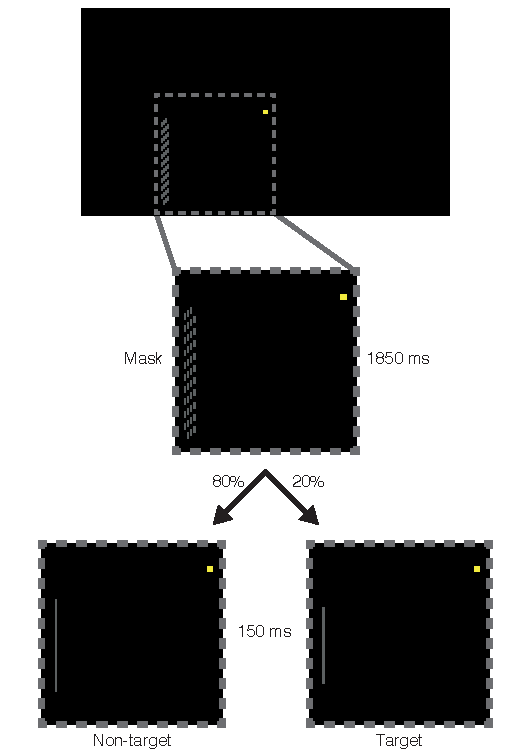
\includegraphics{MFBrain_files/figures/figure_1_task.pdf}
\caption{\label{fig:MFBrain-figure-1-task}\textbf{Sustained attention task}. All stimuli were presented 3° to the left and 1.5° below the yellow fixation square. The inset (dotted square) depicts a zoomed view of the stimuli. Each trial started with the presentation of the mask stimulus for 1850 ms. Then either a non-target (long line; 80\% of trials) or a target (short line; 20\% of trials) was presented for 150 ms. Participants were instructed to only respond to targets.}
\end{figure}

Stimuli were presented at a viewing distance of 110 cm against a black background on a 17-inch Benq TFT monitor, running at a 60 Hz refresh rate. Participants were instructed to maintain fixation on a central yellow square (0.11° x 0.11°), which remained on screen throughout the task. All other stimuli were presented 3° to the left and 1.5° lower than fixation, so participants had to continuously and covertly direct their attention to this location. Every 2000 ms, a light gray line (width: 0.03°) was presented for 150 ms, which could be either short (a target; 20\% of trials) or long (a non-target; 80\% of trials). Participants were tasked to respond with their right index finger whenever they detected a target (short line). Non-targets were always 1.89° long; target length was calibrated individually (see \protect\hyperlink{procedure-1}{Procedure}) for each participant (\emph{M} = 1.40°, \emph{SD} = 0.10°, range = 1.21--1.59°). Line stimuli were preceded and followed by a mask stimulus, presented for the remaining 1850 ms. The mask was composed of many short lines (0.03° x 0.12°), subtending an area of 0.21° by 2.44°. To prevent participants from judging the length of (non-)target lines relative to the mask, the lines that comprised the mask were vertically shifted by a random small amount (within ±0.06°) on each presentation.

\hypertarget{procedure-1}{%
\subsection{Procedure}\label{procedure-1}}

Before the main task, the level at which individual participants performed the task was titrated to achieve a starting point of 80\% accuracy (i.e.~the target was detected 80\% of the time). We did so to equate the task demand across participants and to maximize sensitivity to changes in performance with time-on-task. As in \textcite{MacLean2009}, task difficulty was adjusted by calibrating the length of the target line using Parameter Estimation by Sequential Testing (PEST) \autocite{Taylor1967}. PEST is an adaptive thresholding procedure in which the stimulus is adjusted until a stable level of performance is reached. During the PEST procedure, participants received auditory feedback for incorrect (misses and false alarms) or correct (hits only) responses (a ``ding'' sound for correct; a ``whoosh'' sound for incorrect). The only other difference between the PEST- and main task versions was a higher target rate (PEST: 1 in every 3.5 trials; main task: 1 in 5), to more quickly estimate the threshold target length.

The time it took to complete the PEST procedure varied modestly between participants (range: 7--13 minutes). Afterwards, participants performed 2400 trials (480 target trials) of the main task, which lasted for 80 minutes. No breaks were included, to prevent participants from mitigating the vigilance decrement by taking rest.

There were only two different interruptions of the task. First, before starting the task and every 10 minutes thereafter (after 300 trials), participants rated their levels of motivation (``Please rate your motivation for performing well on this task'') and aversion (``Please rate your aversion towards this task'') on a 7-point scale (1: ``not motivated''/``no aversion'', 7: ``highly motivated''/``strong aversion''). Participants had 6 seconds to do so per rating, by moving a cursor along the scale to the number of their choosing.

Second, after 60 minutes, a new screen was displayed informing participants of the chance to gain an additional monetary reward---an option that was unbeknownst to them until then. This manipulation was designed to evaluate whether motivation could counteract the decline in vigilance over time. Participants could gain €30 on top of their normal compensation, if they outperformed at least 65\% of the other participants during the final 20 minutes of the task (cf. \textcite{Lorist2009}; see Appendix \ref{MFBrain-supplement} for the full instruction text). These instructions were presented for a maximum of 60 seconds, or until the participant indicated they read them by pressing the mouse button. All participants pressed within 60 seconds, after which they rated their motivation and aversion one additional time (such that we could compare these ratings immediately before and after the motivation manipulation) before the task continued.

\hypertarget{behavioral-data-analysis}{%
\subsection{Behavioral data analysis}\label{behavioral-data-analysis}}

We computed \(A'\), a non-parametric index of perceptual sensitivity \autocite{Stanislaw1999}, to assess participants' ability to discriminate targets from non-targets (cf. \textcite{MacLean2009}):

\begin{equation*}
  A' = 0.5 + \frac{(H-F)(1+H-F)}{4H(1-F)}
\end{equation*}

\noindent if \(H > F\), where \(H\) is hit rate (\(Hits / (Hits + Misses)\)) and \(F\) is false alarm rate (\(False\, alarms / (False\, alarms + Correct\, rejections)\)). \(A'\) can take any value between 0.5 (targets are indistinguishable from non-targets) and 1 (perfect discriminability). To track changes in performance over time, \(A'\) was computed for each block of 10 minutes of the experiment (8 blocks in total).

We also analyzed mean response times in hit trials per 10-minute block. Initially, we also planned to analyze the response time coefficient of variation (mean divided by standard deviation), which is known to increase with time-on-task \autocites{Esterman2013}{VanDenBrink2016}. However, precisely estimating the variability in response time requires more trials with responses than we were left with (Hit trials per 10-minute block: \emph{M} = 33, \emph{SD} = 10.5, range = 10--54).

\hypertarget{eeg-data-analysis}{%
\subsection{EEG data analysis}\label{eeg-data-analysis}}

\hypertarget{acquisition-and-preprocessing}{%
\subsubsection{Acquisition and preprocessing}\label{acquisition-and-preprocessing}}

EEG data were recorded at 512 Hz using a BioSemi ActiveTwo system with 64 Ag/AgCl active electrodes, placed according to the (10-10 subdivision of the) international 10-20 system. Two pairs of additional external electrodes were placed to record the EOG, above and below the left eye, and next to the left and right outer canthi.

Preprocessing was performed using the EEGLAB toolbox \autocite{Delorme2004} in MATLAB (Mathworks, Inc.). The continuous EEG data were high-pass filtered at 0.1 Hz using a Hamming-windowed sinc FIR filter. Data were then segmented into epochs from -2000 ms to 3000 ms peri-stimulus (non-targets or targets), including buffer zones on either end to accommodate the edge artifacts that may result from wavelet convolution (see \protect\hyperlink{time-frequency-decomposition}{Time-frequency decomposition}). Epochs containing muscle activity, eye movements or large artifacts due to other sources of noise were removed after visual inspection. Bad channels were interpolated with spherical spline interpolation. Subsequently, independent component analysis was performed on all channels (including the EOG channels). Components consisting of eye blinks or other artifacts clearly distinguishable from neural activity were subtracted from the data. Finally, epochs were average referenced and separated into correct rejections, hits and misses. False alarm trials were too few (only 3\% of non-target trials) to include in the EEG analysis.

\hypertarget{trial-binning}{%
\subsubsection{Trial binning}\label{trial-binning}}

Corresponding to the behavioral data, correct rejection trials were binned into eight blocks of 10 minutes of task performance. We equated trial numbers across blocks for each participant, by discarding a (randomly selected) subset of trials from blocks that had more trials than the minimum. This was done because our inter-trial phase clustering measure (see \protect\hyperlink{time-frequency-decomposition}{Time-frequency decomposition}) in particular can be biased by differences in trial counts between conditions \autocite{Cohen2014}. After this subsampling procedure, an average of 167 correct rejection trials (\emph{SD} = 22.5, range = 124--213) remained per participant for each block. 20-minute bins (4 blocks in total) were used for hit and miss trials, as these were less frequent. Hit and miss trials were also subsampled such that the same amount of hit and miss trials were analyzed per block (\emph{M} = 24, \emph{SD} = 5.4, range = 11-33).

This subsampling procedure was repeated 1000 times; each time a trial-average of each measure (see \protect\hyperlink{event-related-potentials}{Event-related potentials}, \protect\hyperlink{time-frequency-decomposition}{Time-frequency decomposition}) was computed. All 1000 subsampled trial-averages were then averaged together, such that the final value should reflect the average across all trials. The subsampling was repeated in this manner to prevent biases in trial selection, for example because the subsample happened to contain mostly trials from the first half of a block.

\hypertarget{event-related-potentials}{%
\subsubsection{Event-related potentials}\label{event-related-potentials}}

For the ERP analysis, epochs were baseline corrected from -200 to 0 ms pre-stimulus, and averaged separately for each condition. The resulting ERPs were low-pass filtered at a cut-off of 30 Hz (for plotting purposes, for statistical analysis no low-pass filter was applied).

\hypertarget{time-frequency-decomposition}{%
\subsubsection{Time-frequency decomposition}\label{time-frequency-decomposition}}

Time-frequency representations of the EEG data were obtained through complex Morlet wavelet convolution \autocite{Cohen2014}. Wavelet frequency increased from 2 to 80 Hz in 30 logarithmically spaced steps. The number of wavelet cycles was increased from 3 to 12 in the same number of steps, to increase temporal precision at lower frequencies and frequency precision at higher frequencies.

\begin{equation*}
  ITPC_{tf} = \lvert n^{-1} \sum_{r=1}^{n} e^{ik_{tfr}} \rvert
\end{equation*}

\noindent where \(n\) is the number of trials, and \(e^{ik}\) is the complex representation of phase angle \(k\) on trial \(r\) at time-frequency point \(tf\). \(ITPC\) is low when phase values are uniformly distributed across trials (bounded at 0, meaning the phase angle at a certain time is completely random from trial to trial). \(ITPC\) is high when phase angles cluster around a preferred value across trials (bounded at 1, meaning the phase angle at a certain time is exactly the same on each trial).

We also extracted power at each time point and frequency, which was subsequently baseline corrected using a decibel conversion \autocite{Cohen2014}: \(10\log_{10}\ P_{tf}/\overline{baseline_f}\), where \(P_{tf}\) is power at time-frequency point \(tf\) and \(\overline{baseline_f}\) is power at frequency \(f\), averaged across a -400 to -100 ms window relative to stimulus onset.

Finally, to examine spatial attentional bias, we calculated a lateralization index of trial-averaged power values (again per frequency and time point):

\begin{equation*}
  \frac{P_{tf}^{right} - P_{tf}^{left}}{P_{tf}^{right} + P_{tf}^{left}}
\end{equation*}

\noindent where \(P_{tf}^{right}\) is power at time-frequency point \(tf\) at an electrode on the right side of the midline (e.g.~C4) and \(P_{tf}^{left}\) is the equivalent electrode on the left side (e.g.C3). The index is positive when
\(P_{tf}^{right} > P_{tf}^{left}\), and negative for the inverse case. Because this analysis was aimed at examining pre-stimulus power, we did not apply a baseline correction, but instead normalized by total power (\(P_{tf}^{right} + P_{tf}^{left}\)) \autocite[cf.][]{Handel2011}.

\hypertarget{statistical-analysis}{%
\subsection{Statistical analysis}\label{statistical-analysis}}

\(A'\), hit rate, false alarm rate, and response time were analyzed separately using one-way repeated measures ANOVAs with the within-subject factor Block (eight 10-minute blocks of task performance). If the ANOVA revealed a significant effect, we conducted paired t-tests to examine differences between block 1 (first 10 minutes of task performance), block 6 (last block before the motivation manipulation, see \protect\hyperlink{procedure-1}{Procedure}), block 7 (first block after the motivation manipulation), and block 8 (last block of task performance). Specifically, we planned pairwise comparisons of block 1 vs.~block 6, block 1 vs.~block 7, block 6 vs.~block 7, and block 1 vs.~block 8. Bayesian analogues of these t-tests (with a standard Cauchy prior) \autocite{Rouder2009} were used to quantify the relative evidence for an effect (BF\textsubscript{10}) or for the null hypothesis (BF\textsubscript{01}). Motivation and aversion ratings were subjected to a 1x10 repeated measures ANOVA, as there were two ratings in addition to the one after each block: before the task, and directly after the motivation manipulation. For the planned paired tests, these two ratings were used instead of block 1 and block 7.

Similar to the behavioral analyses, EEG data were also subjected to repeated measures ANOVAs with the factor Block. We also followed up each ANOVA with a planned paired test between block 6 and 7, to quantify the effect of motivation. For all EEG analyses, the electrodes, time windows, and frequency windows of interest were determined based on visual inspection of the grand average plots (averaged over participants and blocks) in correct rejection trials.

To examine changes in attentional modulation of early visual processing, our ERP analyses focused on the P1 and N1 components. We extracted average voltage values per participant in a window of 17.5 ms on either side of the P1 and N1 peak. For each participant, the P1 peak latency was defined as the sample with the maximum (positive) voltage within 110--180 ms post-stimulus; N1 peak latency was defined as the sample with the minimum (negative) voltage within 190--260 ms post-stimulus. These values were averaged for two pools of electrodes: left parieto-occipital (PO5, P5, P7) and right parieto-occipital (PO6, P6, P8). We ran separate repeated measures ANOVAs for the P1 and N1: an 8 (Block) x 2 (Hemisphere: left PO vs.~right PO) ANOVA for correct rejection trials, and another 4 (Block) x 2 (Hemisphere) x 2 (Condition: hits vs.~misses) ANOVA.

To examine changes in attentional stability, we analyzed ITPC values for the same left PO and right PO electrode pools, as well as a mid-frontal (MF) pool of electrodes (FCz, FC1, FC2). Similar to the ERP analysis, we extracted average values for statistics using participant-specific windows of 60 ms and 1 Hz on either side of the peak value for that participant, within a larger window of 150--500 ms and 3--7 Hz (consistent across participants). We again ran two repeated measures ANOVAs: an 8 (Block) x 3 (Region: left PO vs.~right PO vs.~MF) ANOVA for correct rejection trials, and another 4 (Block) x 3 (Region) x 2 (Condition: hits vs.~misses) ANOVA. We also analyzed theta power, using the exact same electrodes, time-frequency windows, and ANOVA factors.

In an additional post hoc analysis, we quantified the relationship over time between ITPC and \(A'\) using a multilevel growth model. Multilevel growth models are an extension of linear mixed models that can accommodate hierarchical data structures \autocite[see e.g.][]{Kristjansson2007}. A multilevel growth model is appropriate in our case, because changes over time in variables at one level (ITPC, \(A'\)) are nested within another level (participants). Specifically, we modeled ITPC per 10-minute block as a fixed effect and \(A'\) per block as the outcome. To account for the correlation between repeated measures, we specified a first-order auto-regressive covariance structure between the 8 blocks, nested within participants.

Finally, to examine changes in preparatory attentional orienting, we extracted the average pre-stimulus (-1000 to -100 ms) power lateralization index values in the alpha range (9--14 Hz), again from the left PO and right PO electrode pools, and subjected these to 1x8 (Block) (correct rejections) and 4 (Block) x 2 (Condition: hits vs.~misses) repeated measures ANOVAs.

All statistical analyses were conducted using several R \autocite{R-base} packages \autocites{R-ez}{R-BayesFactor}{R-nlme}{R-broom}{R-tidyverse} from within RStudio \autocite{RStudio2016}. Effect sizes are reported as (partial) eta-squared (\(\eta^{2}_{p}\)) or Cohen's \emph{d}. \(\alpha\) was fixed at 0.05. In case Mauchly's test for violations of sphericity was significant, we report Greenhouse-Geisser corrected p-values and degrees of freedom.

\hypertarget{data-materials-and-code-availability-3}{%
\subsection{Data, materials, and code availability}\label{data-materials-and-code-availability-3}}

The data, materials, and analysis code can be obtained from this study's page on the \href{https://doi.org/10.17605/OSF.IO/EMF9H}{Open Science Framework}, including: The raw behavioral data, as well as the raw and preprocessed EEG data \autocite{Reteig2018a}; An R notebook \autocite{R-knitr} that reproduces all of the statistical results in this publication; MATLAB scripts that reproduce all the figures in this publication; MATLAB code to compute the EEG measures from the preprocessed EEG data and extract the data for statistics.

\hypertarget{MFBrain-results}{%
\section{Results}\label{MFBrain-results}}

\hypertarget{behavior}{%
\subsection{Behavior}\label{behavior}}

The sustained attention task elicited a robust vigilance decrement: accuracy in discriminating targets from non-targets (defined as \(A'\)) decreased with time-on-task (Figure \ref{fig:figure-2-behav}A, \emph{F}(2.50, 49.96) = 7.47, \emph{p} \textless{} .001, \(\eta^2\) = .27). Accuracy declined rapidly until around 30 minutes into the task, when it became more or less stable. Response times also followed this pattern, but stabilized earlier (Figure \ref{fig:figure-2-behav}B, \emph{F}(3.82, 76.45) = 2.56, \emph{p} = .047, \(\eta^2\) = .11). With time-on-task, motivation to continue decreased (Figure \ref{fig:figure-2-behav}E, \emph{F}(3.89, 77.80) = 7.10, \emph{p} \textless{} .001, \(\eta^2\) = .26), while aversion ratings increased (Figure \ref{fig:figure-2-behav}F, \emph{F}(3.46, 69.17) = 12.67, \emph{p} \textless{} .001, \(\eta^2\) = .39).

After one hour (after block 6), participants learned that they could earn an additional sum of money if they outperformed at least 65\% of the other participants during the final 20 minutes of the task. Just before this manipulation, motivation was at its lowest (begin vs.~6: \emph{M\textsubscript{diff}} = 1.52, \emph{t}(20) = 3.55, \emph{p} = .002, \emph{d} = 0.78, BF\textsubscript{10} = 19.9), and aversion was at its peak (begin vs.~6: \emph{M\textsubscript{diff}} = -2.67, \emph{t}(20) = -6.16, \emph{p} \textless{} .001, \emph{d} = -1.34, BF\textsubscript{10} = 4057). Right after the motivation manipulation, participants were significantly more motivated compared to before (6 vs.~post: \emph{M\textsubscript{diff}} = -2.10, \emph{t}(20) = -5.14, \emph{p} \textless{} .001, \emph{d} = -1.12, BF\textsubscript{10} = 515), and also displayed decreased aversion towards performing the task (6 vs.~post: \emph{M\textsubscript{diff}} = 0.67, \emph{t}(20) = 3.16, \emph{p} = .005, \emph{d} = 0.69, BF\textsubscript{10} = 9.2). Motivation ratings were no longer significantly different from the beginning (begin vs.~post: \emph{M\textsubscript{diff}} = -0.57, \emph{t}(20) = -1.74, \emph{p} = .097, \emph{d} = -0.38, BF\textsubscript{01} = 1.21), and remained at this level after the final two blocks (begin vs.~8: \emph{M\textsubscript{diff}} = 0.76, \emph{t}(20) = 1.82, \emph{p} = .084, \emph{d} = 0.40, BF\textsubscript{01} = 1.09).

The motivation manipulation improved accuracy in the following block of task performance (6 vs.~7: \emph{M\textsubscript{diff}} = -0.024, \emph{t}(20) = -2.51, \emph{p} = .021, \emph{d} = -0.55, BF\textsubscript{10} = 2.75). However, accuracy was still significantly lower than the first block (1 vs.~7: \emph{M\textsubscript{diff}} = 0.029, \emph{t}(20) = 2.40, \emph{p} = .026, \emph{d} = 0.52, BF\textsubscript{10} = 2.28), and reached its lowest point overall in the final ten minutes of task performance (1 vs.~8: \emph{M\textsubscript{diff}} = 0.062, \emph{t}(20) = 4.23, \emph{p} \textless{} .001, \emph{d} = 0.92, BF\textsubscript{10} = 79.2), despite equal levels of self-reported motivation. These changes in \(A'\) appeared to be mostly driven by hit rate (Figure \ref{fig:figure-2-behav}C), as hit rate also worsened significantly with time-on-task (\emph{F}(2.45, 48.92) = 8.74, \emph{p} \textless{} .001, \(\eta^2\) = .30), and improved transiently after the motivation manipulation (6 vs.~7: \emph{M\textsubscript{diff}} = -0.077, \emph{t}(20) = -2.17, \emph{p} = .042, \emph{d} = -0.47, BF\textsubscript{10} = 1.56). False alarm rate appeared to decrease slightly over time (Figure \ref{fig:figure-2-behav}D), but not significantly (\emph{F}(3.08, 61.69) = 2.30, \emph{p} = .084, \(\eta^2\) = .10), and was also not significantly affected by motivation (6 vs.~7: \emph{M\textsubscript{diff}} = 0.006, \emph{t}(20) = 1.10, \emph{p} = .286, \emph{d} = 0.24, BF\textsubscript{01} = 2.59). False alarms were rare, as false alarm rate was already near the floor at the start of the experiment (3.1\% of non-target trials). Finally, although response time showed the same pattern as accuracy (Figure \ref{fig:figure-2-behav}B), response time did not significantly change after the motivation manipulation (6 vs.~7: \emph{M\textsubscript{diff}} = 22, \emph{t}(20) = 1.45, \emph{p} = .163, \emph{d} = 0.32, BF\textsubscript{01} = 1.78).

\newpage
\pagestyle{empty}
\changetext{}{}{}{-12.5mm}{}
\blandscape
\captionsetup{width=\linewidth}



\begin{figure}
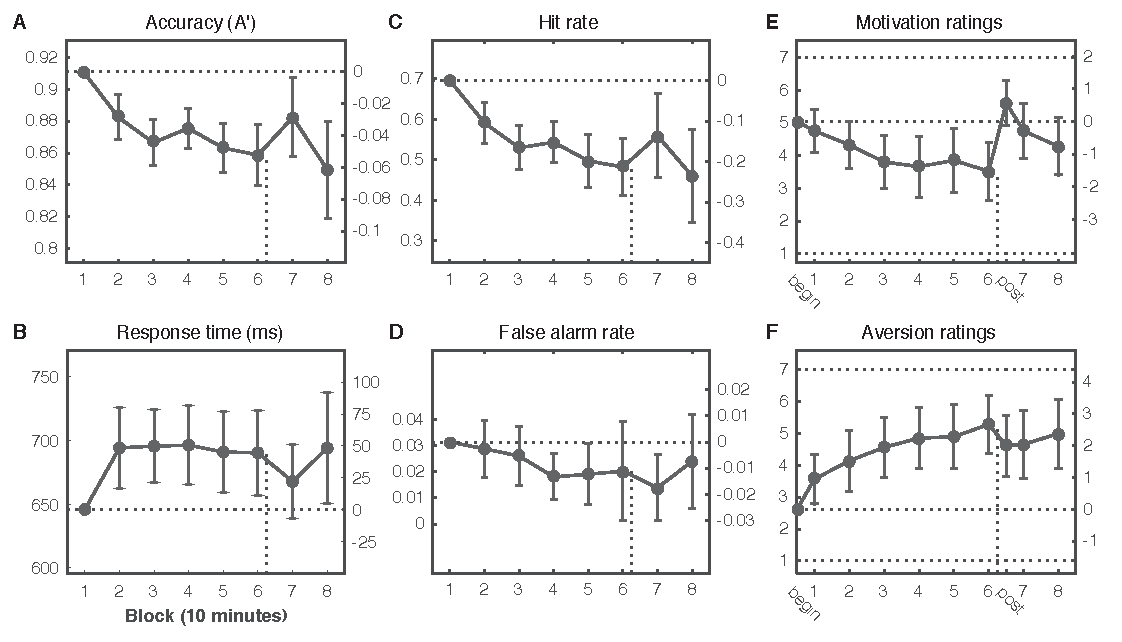
\includegraphics[width=190mm]{MFBrain_files/figures/figure_2_behav} \caption{\textbf{Declining performance with time-on-task is only partially counteracted by increases in motivation}. (\textbf{A}) Accuracy (\(A'\)) declined with time on task and was only partially and transiently restored by the motivation manipulation (after 60 minutes of task performance; vertical dotted line). These changes in accuracy were mirrored in the response time data (\textbf{B}) and mostly due to changes in Hit rate (\textbf{C}); there was no significant change over time in False alarm rate (\textbf{D}). The motivation manipulation successfully restored motivation ratings to their initial levels (\textbf{E}), but aversion ratings (\textbf{F}) remained elevated. The left y-axis of each plot shows the absolute value; the right y-axis shows the change compared to the first measurement (horizontal dotted line). Error bars are 95\% confidence intervals of the paired difference between the first and each subsequent mean; paired differences are significant when the confidence interval does not overlap the dotted line. The x-axis depicts time-on-task in blocks of 10 minutes. The motivation and aversion ratings (horizontal dotted lines: minimum of 1, maximum of 7) were taken after each block (1 through 8), as well as before the task started (\emph{begin}) and directly after the motivation manipulation (\emph{post}).}\label{fig:figure-2-behav}
\end{figure}

\newpage
\elandscape
\changetext{}{}{}{+12.5mm}{}
\pagestyle{\defstyle}
\captionsetup{width=\textwidth}

\hypertarget{attentional-stability-theta-phase}{%
\subsection{Attentional stability: theta phase}\label{attentional-stability-theta-phase}}

Inter-trial phase clustering (ITPC) indexes the consistency in timing with which frequency-band-limited activity is elicited from trial to trial. Theta-band ITPC has been interpreted as a marker of attentional stability \autocite{Lutz2009}. We therefore hypothesized that theta-band ITPC would decrease with time-on-task. Our data show clear ITPC in a theta-band (3--7 Hz) response from 150--500 ms post-stimulus (Figure \ref{fig:figure-3-theta}A). The response was maximal over left and right parieto-occipital (lPO, rPO) electrodes, as well as over mid-frontal (MF) scalp sites (Figure \ref{fig:figure-3-theta}B).

Over the course of the eight task blocks, theta ITPC closely tracked the time course of behavioral task performance (accuracy in \(A'\)) (Figure \ref{fig:figure-3-theta}C). Like behavioral performance, theta ITPC decreased with time-on-task (\emph{F}(3.83, 76.52) = 4.46, \emph{p} = .003, \(\eta^2_p\) = .18) and increased directly after the motivation manipulation at two out of the three scalp regions (left PO, 6 vs.~7: \emph{t}(20) = -3.56, \emph{p} = .002, \emph{d} = -0.78, BF\textsubscript{10} = 20.1; right PO, 6 vs.~7: \emph{t}(20) = -1.94, \emph{p} = .067, \emph{d} = -0.42, BF\textsubscript{10} = 1.09; MF, 6 vs.~7: \emph{t}(20) = -3.13, \emph{p} = .005, \emph{d} = -0.68, BF\textsubscript{10} = 8.64).

To more directly quantify the relationship between theta ITPC and \(A'\) over time, we fitted a multilevel growth model wherein we regressed the \(A'\) scores on the ITPC scores in correct rejection trials. This analysis showed that ITPC significantly predicted \(A'\) over time (left PO: \emph{b} = 0.11, \emph{t}(166) = 3.11, \emph{p} = .002; right PO: \emph{b} = 0.12, \emph{t}(166) = 3.89, \emph{p} \textless{} .001; MF: \emph{b} = 0.15, \emph{t}(166) = 4.39, \emph{p} \textless{} .001). ITPC was also larger in hit than in miss trials (Figure \ref{fig:figure-3-theta}D, \emph{F}(1, 20) = 58.31, \emph{p} \textless{} .001, \(\eta^2_p\) = .74), which further corroborates that the theta ITPC signal was relevant for behavior. This difference between hits and misses did not change significantly over time (no Block by Condition interaction, \emph{F}(3, 60) = 1.39, \emph{p} = .254, \(\eta^2_p\) = .07).

\newpage
\pagestyle{empty}
\changetext{}{}{}{-12.5mm}{}
\blandscape
\captionsetup{width=190mm}



\begin{figure}
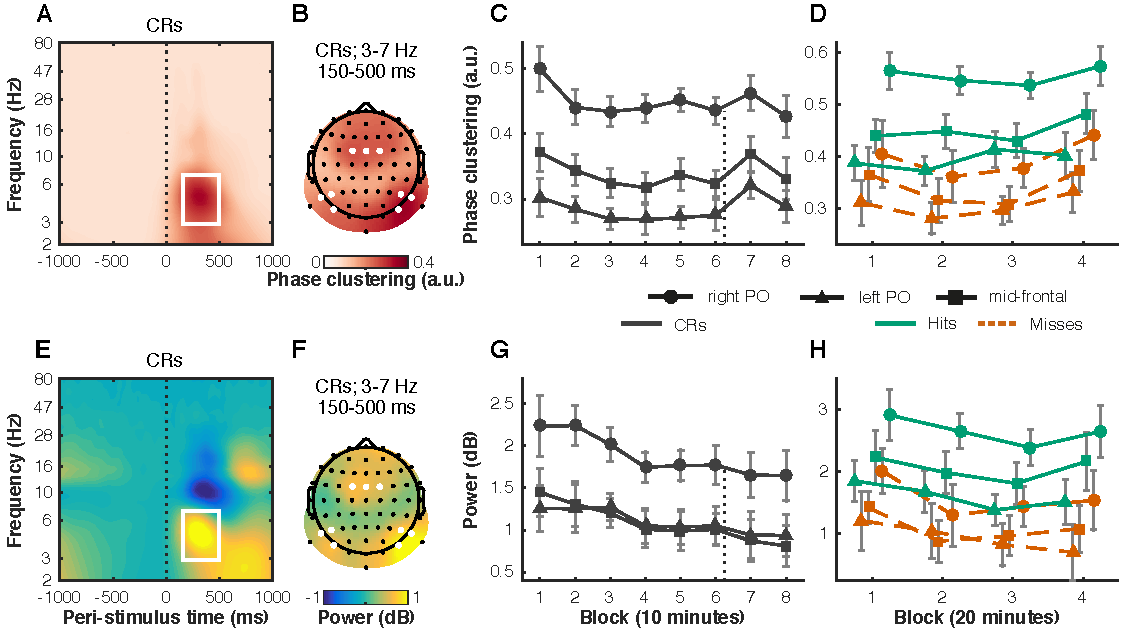
\includegraphics[width=190mm]{MFBrain_files/figures/figure_3_theta} \caption{\textbf{Changes in behavioral performance with time-on-task and motivation are closely tracked by cross-trial consistency of post-stimulus theta phase (A--D), but not theta power (E--H)}. Theta inter-trial phase clustering (ITPC) peaked from 150--500 ms post-stimulus (vertical dotted-line) between 3 and 7 Hz (time-frequency window outlined in white) (\textbf{A}, average of electrodes of interest) on left parieto-occipital (left PO) electrodes (PO7, P5, P7), right parieto-occipital (right PO) electrodes (PO8, P6, P8), and mid-frontal (MF) electrodes (FC1, FCz, FC2) (\textbf{B}, average of time-frequency window, electrodes marked in white). The same electrode sites and time-frequency windows of interest were used for theta power (\textbf{E}, \textbf{F}), baseline corrected from -400 to -100 ms using a decibel conversion. Theta ITPC in correct rejection trials (CRs) decreased with time-on-task (8 blocks of 10 minutes each) and increased after the motivation manipulation (directly after block 6; vertical dotted line) (\textbf{C}), closely resembling changes in task performance (Figure \ref{fig:figure-2-behav}A). Power in the theta band decreased linearly over time, but did not change after the motivation manipulation (\textbf{G}). Both theta ITPC (\textbf{D}) and power (\textbf{H}) were higher for hit than miss trials, but this difference did not change significantly over time (4 blocks of 20 minutes each). Error bars are within-subject \autocites{Cousineau2005}{Morey2008} 95\% confidence intervals.}\label{fig:figure-3-theta}
\end{figure}

\newpage
\elandscape
\changetext{}{}{}{+12.5mm}{}
\pagestyle{\defstyle}
\captionsetup{width=\textwidth}

We also investigated to what extent dynamics in theta power were similar to theta ITPC. Unsurprisingly, we observed a theta power response in the same time-frequency window and electrode sites (Figure \ref{fig:figure-3-theta}E--F). Like theta ITPC, theta power decreased over time in correct rejection trials (Figure \ref{fig:figure-3-theta}G, \emph{F}(3.04, 60.85) = 4.91, \emph{p} = .004, \(\eta^2_p\) = .20). Theta power also differed between hits and misses (Figure \ref{fig:figure-3-theta}H, \emph{F}(1, 20) = 43.02, \emph{p} \textless{} .001, \(\eta^2_p\) = .68). This difference did not change significantly over time (no Block by Condition interaction, \emph{F}(3, 60) = 1.04, \emph{p} = .383, \(\eta^2_p\) = .05). However, unlike theta ITPC, theta power was not significantly affected by the motivation manipulation (left PO, 6 vs.~7: \emph{p} = .525, BF\textsubscript{01} = 3.64; right PO, 6 vs.~7: \emph{p} = .409, BF\textsubscript{01} = 3.20; MF, 6 vs.~7: \emph{p} = .214, BF\textsubscript{01} = 2.14).

In sum, theta-band inter-trial phase clustering was higher in hit than in miss trials, suggesting it indexes behavioral performance. Changes in theta ITPC in correct rejection trials were tightly coupled to and predicted changes in behavioral performance (\(A'\)). Power in the theta band also decreased over time, but did not appear to respond to the motivation manipulation, suggesting that the change in power with time-on-task was partially independent of and less strongly associated with behavior than theta ITPC.

\hypertarget{early-visual-processing-p1-and-n1-components}{%
\subsection{Early visual processing: P1 and N1 components}\label{early-visual-processing-p1-and-n1-components}}

To investigate how time-on-task and motivation may affect early visual processing, we examined how the P1 (Figure \ref{fig:figure-4-ERPs}A--D) and N1 (Figure \ref{fig:figure-4-ERPs}E-H) ERP components evolved over the eight task blocks (i.e., in correct rejection trials). N1 amplitude decreased over time (Figure \ref{fig:figure-4-ERPs}G, \emph{F}(2.89, 57.75) = 5.79, \emph{p} = .002, \(\eta^2_p\) = .22), but there was no significant effect of Block for the P1 (Figure \ref{fig:figure-4-ERPs}C, \emph{F}(3.68, 73.70) = 1.16, \emph{p} = .333, \(\eta^2_p\) = .06). The N1 did not change significantly after the motivation manipulation, neither in the left hemisphere (6 vs.~7: \emph{t}(20) = 0.73, \emph{p} = .472, \emph{d} = 0.16, BF\textsubscript{01} = 3.45) nor in the right (6 vs.~7: \emph{t}(20) = -0.33, \emph{p} = .742, \emph{d} = -0.07, BF\textsubscript{01} = 4.18), suggesting that the decrease in the N1 with time-on-task is not sensitive to motivation, and may reflect other factors such as habituation to the repeatedly presented stimulus.

\newpage
\pagestyle{empty}
\changetext{}{}{}{-12.5mm}{}
\blandscape
\captionsetup{width=\linewidth}



\begin{figure}
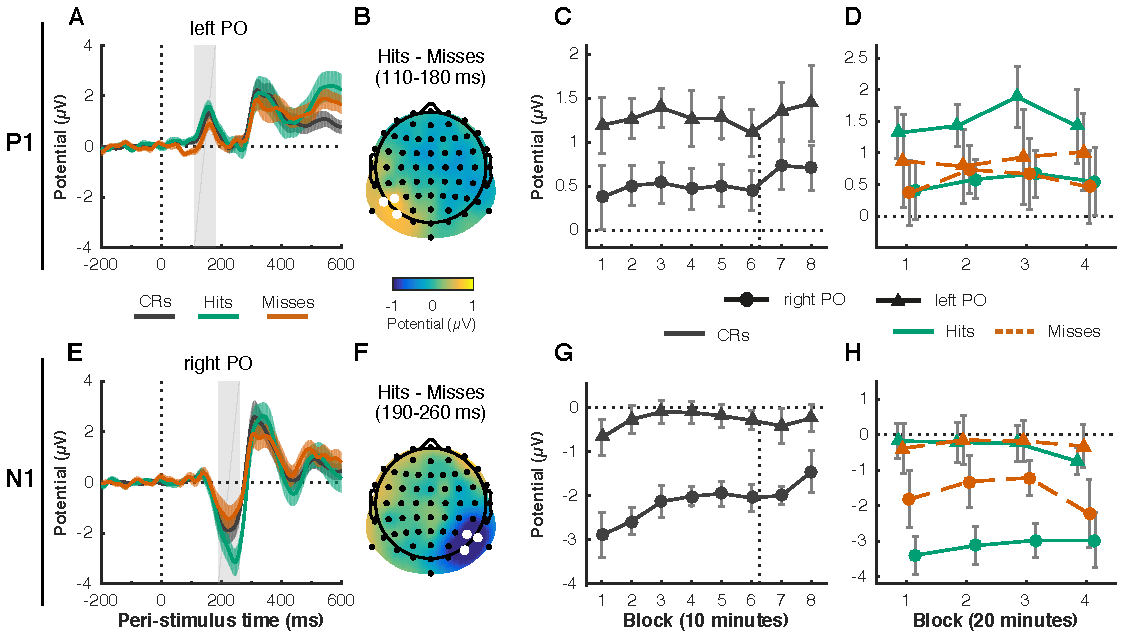
\includegraphics[width=190mm]{MFBrain_files/figures/figure_4_ERPs} \caption{\textbf{Time-on task and motivation do not affect attentional modulation of early visual processing: P1 (A-D) and N1 (E-H) ERP components}. The P1 peaked between 110--180 ms (gray shaded rectangle) post-stimulus (vertical dotted line) on left parieto-occipital (left PO) electrodes (PO7, P5, P7) (\textbf{A}). The N1 peaked between 190--260 ms (gray shaded rectangle) on right parieto-occipital (right PO) electrodes (PO8, P6, P8) (\textbf{E}). The attentional modulation of the components, defined as the difference between hits and misses, was also lateralized to the left PO region for the P1 (\textbf{B}, average of P1 time window, left PO electrodes marked in white) and the right PO region for the N1 (\textbf{F}, average of N1 time window, right PO electrodes marked in white). P1 amplitude (\textbf{C}) did not change significantly over time in correct rejection (CR) trials, but N1 amplitude did decrease with time-on-task (\textbf{G}) (8 blocks of 10 minutes each). The time of the motivation manipulation (directly after block 6) is indicated with the vertical dotted line. There was no significant change in the attentional modulation (hits vs.~misses) of the P1 (\textbf{D}) and N1 (\textbf{H}) over time (4 blocks of 20 minutes each). Error bars are within-subject \autocites{Cousineau2005}{Morey2008} 95\% confidence intervals; shaded areas in (A) and (E) represent the standard error of the mean.}\label{fig:figure-4-ERPs}
\end{figure}

\newpage
\elandscape
\changetext{}{}{}{+12.5mm}{}
\pagestyle{\defstyle}
\captionsetup{width=\textwidth}

The ANOVA for correct rejection trials also revealed main effects of Hemisphere, reflecting that the P1 was only visible over a left parieto-occipital scalp region (\emph{F}(1, 20) = 13.07, \emph{p} = .002, \(\eta^2_p\) = .40), whereas the N1 peaked exclusively over the right parieto-occipital scalp region (\emph{F}(1, 20) = 15.28, \emph{p} \textless{} .001, \(\eta^2_p\) = .43). This unusual lateralization of the components is further explored elsewhere \autocite{Slagter2016}. Briefly, we found that this effect could be attributed to the specific stimulus used, as well as the fact that participants were continuously attending to the left hemifield, and the right hemifield was never relevant (which differs from typical attentional cueing studies).

As top-down attention is known to increase the amplitudes of the P1 and N1, we also examined the difference between hit and miss trials, as a proxy for attentional modulation. We hypothesized that with time on task, top-down attentional modulation of these indices of visual processing would decrease. The attentional modulations of both components were also completely lateralized (Condition by Hemisphere interaction), as both the P1 and N1 amplitude were larger for hits than misses, but only in the left and right hemisphere, respectively (P1: Figure \ref{fig:figure-4-ERPs}B, \emph{F}(1, 20) = 7.48, \emph{p} = .013, \(\eta^2_p\) = .27; N1: Figure \ref{fig:figure-4-ERPs}F, \emph{F}(1, 20) = 11.86, \emph{p} = .003, \(\eta^2_p\) = .37). However, this effect did not interact with Block, suggesting that the attentional modulation of visual processing did not change over time or after the motivation instruction (P1: Figure \ref{fig:figure-4-ERPs}D, \emph{F}(3, 60) = 0.53, \emph{p} = .664, \(\eta^2_p\) = .03; N1: Figure \ref{fig:figure-4-ERPs}H, \emph{F}(3, 60) = 1.70, \emph{p} = .177, \(\eta^2_p\) = .08).

In sum, N1 amplitude decreased with time-on-task (in correct rejection trials), but appeared to be unaffected by the motivation manipulation. The P1 and N1 components and attentional modulations thereof were completely lateralized: the P1 dissociated between hits and misses in the irrelevant hemisphere (left); the N1 dissociated between hits and misses in the relevant hemisphere (right) \autocite[see][]{Slagter2016}. However, this pattern did not change significantly with time-on-task or motivation.

\hypertarget{preparatory-attentional-orienting-alpha-power}{%
\subsection{Preparatory attentional orienting: alpha power}\label{preparatory-attentional-orienting-alpha-power}}

Next to processing of the stimulus itself, we also asked whether time-on-task might degrade preparatory attentional processes. Spatial cues that signal the location of an upcoming stimulus are known to affect the distribution of oscillatory alpha power. Specifically, alpha power decreases over the hemisphere contralateral to the attended location, and increases over the ipsilateral hemisphere. Because stimuli only appeared in the left hemifield in our task, we expected to see higher alpha power over the left (ipsilateral) hemisphere. We also expected to see this lateralization decay over time, as participants became less able to direct their attention in preparation of the stimulus.

However, both of these predictions were not borne out. First, we consistently observed higher power in a 9--14 Hz band over the right parieto-occipital scalp site than over the left (Figure \ref{fig:figure-5-latindex}A--B). Because we predicted exactly the opposite (higher alpha power over the left hemisphere), the alpha lateralization we observed here likely does not index top-down attentional orienting. Instead, like the unexpected lateralization in the P1 and N1 components, this inverse alpha asymmetry is probably due to our unorthodox task design where only the left hemifield was ever relevant \autocite[as further discussed in][]{Slagter2016}, and likely reflects a resting state pattern \autocites{Benwell2018}{Wieneke1980}.

Second, this deviant pattern of alpha lateralization did not change with time-on-task (Figure \ref{fig:figure-5-latindex}C, \emph{F}(3.52, 70.42) = 0.94, \emph{p} = .438, \(\eta^2\) = .04, nor was it affected by the motivation manipulation (6 vs.~7: \emph{t}(20) = 0.10, \emph{p} = .920, \emph{d} = 0.02, BF\textsubscript{01} = 4.38). Alpha lateralization was significantly larger in miss compared to hit trials (Figure \ref{fig:figure-5-latindex}D, \emph{F}(1, 20) = 12.68, \emph{p} = .002, \(\eta^2_p\) = .39) \autocite{Slagter2016}, but this difference did not change significantly over time (no Block by Condition interaction, \emph{F}(3, 60) = 0.46, \emph{p} = .708, \(\eta^2_p\) = .02.

In sum, although only one hemifield (the left) was ever relevant, we observed higher alpha power over the processing hemisphere (on the right) than the non-processing hemisphere (on the left), which is exactly opposite to the canonical pattern. This deviant alpha lateralization remained stable over time.



\newpage
\pagestyle{empty}
\blandscape

\begin{figure}
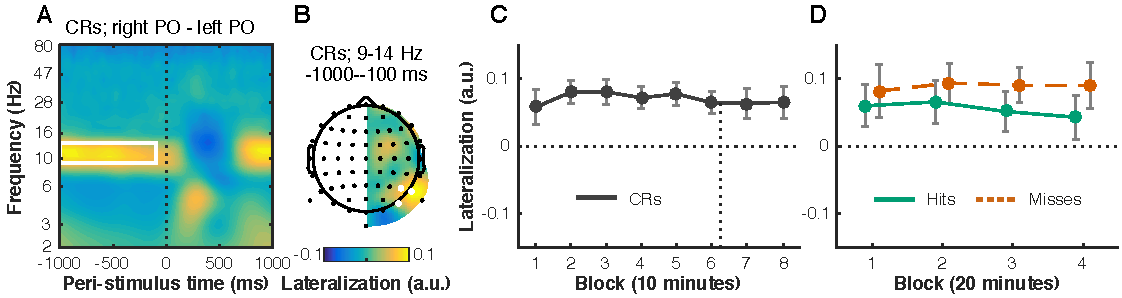
\includegraphics[width=190mm]{MFBrain_files/figures/figure_5_latindex} \caption{\textbf{Pre-stimulus alpha power remains right-lateralized over time, despite stimuli appearing exclusively in the left visual hemifield}. For each time-frequency point, we computed a lateralization index, by subtracting power at each left electrode from its counterpart on the right side, and dividing by the sum. Positive values therefore mean that power was relatively stronger over the right hemisphere. Our data show that pre-stimulus (vertical dotted line) alpha power is right-lateralized (\textbf{A}, time-frequency window: 9--14 Hz, -1000 to -100 ms, outlined in white), when comparing left (PO7, P5, P7) and right parieto-occipital (right PO: PO8, P6, P8) electrode sites (\textbf{B}, electrodes marked in white). This pattern did not change significantly with time-on-task, neither in correction rejection trials (CRs) (\textbf{C}, 8 blocks of 10 minutes each; time of the motivation manipulation indicated with vertical dotted line), nor in hit and miss trials (\textbf{D}, 4 blocks of 20 minutes each). Error bars are within-subject \autocites{Cousineau2005}{Morey2008} 95\% confidence intervals.}\label{fig:figure-5-latindex}
\end{figure}

\newpage
\elandscape
\pagestyle{\defstyle}

\hypertarget{MFBrain-discussion}{%
\section{Discussion}\label{MFBrain-discussion}}

We aimed to study changes in control of attention as a function of prolonged task performance, and the extent to which these could be explained by changes in motivation. Our participants performed a demanding sustained attention task for 80 minutes, and received an unexpected motivation boost after 60 minutes. We found that performance rapidly declined (i.e.~the classic vigilance decrement / time-on-task effect) before the motivation boost. Afterwards, task performance did increase, but only partially (not up to the initial level) and transiently (not for the full remaining 20 minutes), even though self-reported motivation remained at initial levels.

We also recorded EEG to investigate whether changes in behavioral performance over time were accompanied by changes in three markers of attentional control. We examined pre-stimulus lateralization of alpha power as an index of preparatory orienting of attention, but did not find the canonical pattern of lateralization, nor any effect of time-on-task or motivation. In addition, the attentional modulation of the early visual P1 and N1 ERP components also did not change with time-on-task or motivation, though the absolute amplitude of the N1 decreased over time. Finally, in contrast, changes in theta-band inter-trial phase clustering (ITPC) between 150--500ms post-stimulus were closely coupled to the changes in behavioral performance following time-on-task and motivation. Given that ITPC indexes the temporal consistency of neural responses across trials \autocite{VanRullen2011}, the readiness of the attentional system to respond to incoming input might reduce with time-on-task. Collectively, our results thus suggest that changes in performance during sustained attention tasks are most closely associated with fluctuations in the stability of later-stage attentional processes.

\hypertarget{motivation-partially-and-transiently-restores-vigilance}{%
\subsection{Motivation partially and transiently restores vigilance}\label{motivation-partially-and-transiently-restores-vigilance}}

The sustained attention task induced a robust vigilance decrement: performance rapidly decreased with time-on-task, reaching a plateau after 20--30 minutes of task performance. After 60 minutes, we motivated our participants with an extra sum of money if they would outperform 65\% of the other participants for the final 20 minutes. This prospect successfully increased self-rated levels of motivation. The motivation boost counteracted the vigilance decrement, as task performance increased in the 10-minute block immediately after participants learned of the reward. This appears inconsistent with the overload framework, which proposes that the vigilance decrement occurs due to depletion of resources---motivation alone should not be sufficient to replenish them.

However, motivation was also not enough to completely stave off the vigilance decrement, as performance was still lower than at the beginning of the task. In addition, participants appeared unable to sustain their new-found stamina: performance in the final block dropped back down to the lowest level overall. So perhaps resource depletion still played a role: participants simply could not keep up their performance, even though they were strongly incentivized to do so and self-reported to be as motivated as they were at the beginning of the task (though our Bayes factor analysis did not show strong evidence for the latter). Our findings are thus in partial agreement with both overload and motivational control accounts of the vigilance decrement.

Previous studies also found mixed evidence for the efficacy of motivation in restoring performance. In some cases, accuracy \autocite{Hopstaken2015} and response time \autocites{Boksem2006}{Lorist2009} can recover after unexpected rewards, sometimes up to or beyond the initial levels. However, all of these studies measured performance at only one time point following the manipulation, so it is unknown whether performance subsequently declined---as we observed here. In contrast, two other studies have found that the slope of the vigilance decrement is not affected by low- or high reward levels \autocites{Esterman2014}{Gergelyfi2015}.

The main difference is that these latter two studies used trial-based rewards, which may decrease in value over time \autocite{Fortenbaugh2017}. Indeed, participants appear to discount the value of rewards when they have to pay the ``cost'' of sustaining their attention for longer \autocite{Massar2016}. The same goes for losses instead of rewards: when losses are small and continuous, the vigilance decrement occurs as normal. But when the risk of an instantaneous and large loss looms, the vigilance decrement can in fact be partially attenuated \autocite{Esterman2016}.

These observations are in line with motivational control theories \autocites{Hockey1997}{Kurzban2013}, stating that participants are only motivated to keep up performance when benefits outweigh the costs. Note that the level of available resources may still be a principal factor in this cost/benefit computation \autocites{Boksem2008}{Christie2015}. Perhaps the pattern of performance we observed---a transient increase with motivation, and a subsequent dip---also occurred because participants re-evaluated the cost/benefit ratio during the final stretches of task performance. Indeed, self-reported motivation dropped down again after the initial motivation boost, although motivation did not become significantly lower than at the start of the task.

We highlight two further caveats to our conclusion that motivation can increase performance after the initial vigilance decrement. First, we quantified performance as perceptual sensitivity (\(A'\)), which should exclusively reflect participants' ability to discriminate targets from non-targets, not other factors such as response bias (the overall tendency for participants to respond `yes' or `no'). However, \textcite{Thomson2016} argue that with the very low false alarm rates that vigilance tasks typically exhibit, sensitivity and response bias cannot be fully teased apart. Indeed, false alarm rate in our study was almost at floor and did not change significantly with time-on-task, so we cannot exclude that the effect on sensitivity is partially driven by response bias as well. Note that overload accounts imply a specific sensitivity decrease, but underload accounts do not necessarily.

Second, the effect that the motivation manipulation had on performance might not result from motivation per se, but due to there being a short break in the task: the 1-minute maximum period the participants had to read the instruction. Even short breaks are known to increase performance \autocite{Helton2015}, though performance can also decrease more in subsequent task blocks after a break \autocite{Lim2015}. This pattern matches the changes in performance we observed after the motivation manipulation. From a strong overload perspective, one could argue that the rest afforded by the break is what caused performance to restore, and that the motivation boost played no causal role. However, the resting opportunity was very brief---all participants resumed the task within one minute---whereas these studies examined breaks of at least a minute, and much longer. Interestingly, \textcite{Ross2014} examined the effect of 1-minute breaks in a task very similar to ours (line length discrimination). They show that breaks are effective if they occur earlier in the vigil (after 20 minutes), but not later (after 30 minutes). Because the break in our task occurred much later (after 60 minutes), the findings of \textcite{Ross2014} argue against the interpretation that the subsequent increase in performance was simply due to rest.

\hypertarget{theta-inter-trial-phase-clustering-mirrors-effects-of-time-on-task-and-motivation-on-behavioral-performance}{%
\subsection{Theta inter-trial phase clustering mirrors effects of time-on-task and motivation on behavioral performance}\label{theta-inter-trial-phase-clustering-mirrors-effects-of-time-on-task-and-motivation-on-behavioral-performance}}

Out of our three EEG measures, post-stimulus theta ITPC was most clearly associated with prolonged performance on the sustained attention task. Theta (3--7 Hz) ITPC was larger when the target was successfully detected (hits) than when it was missed, suggesting that it indexes a behaviorally relevant process. Changes in theta ITPC closely tracked changes in behavioral performance---both those due to time-on-task as well as motivation. Theta ITPC diminished with time-on-task, which means that the timing of the neural response across trials became more variable. The increased variability might reflect that participants became progressively less able to prepare for the onset of the visual stimulus by attending at the right moment in time. We thus interpret theta ITPC as a measure of attentional stability, following previous work \autocites{Lutz2009}{Slagter2009}. Besides time-on-task, other factors may influence attentional stability: theta ITPC also increased after the motivation manipulation. An earlier study demonstrated that theta ITPC also decreases when participants are mind wandering \autocite{Baird2014}.

Oscillatory activity in the theta band is known to occur in frontal and parietal areas in visual attention tasks \autocite{Demiralp1992}, particularly when attention has to be sustained \autocite{Clayton2015}. The theta-band response in our study was observed over bilateral parieto-occipital electrodes, but also a mid-frontal scalp site. Of course, no conclusions on the source of this activity can be drawn based on the scalp topography, but it is possible that anterior and posterior theta-band activity reflect different processes. Frontal mid-line theta is strongly associated with cognitive control processes such as action monitoring, and likely originates from the anterior cingulate cortex \autocites{Cavanagh2014}{Narayanan2013}. However, these theta-band signals are ongoing oscillations that are not phase-locked to external stimuli \autocite{Cohen2013}, while the theta ITPC response we observe appears to be strongly phase-locked to the eliciting stimulus. Posterior theta-band activity is often observed following (any) visual stimuli \autocite{Klimesch2007}. Theta ITPC is stronger for unexpected targets, suggesting it is particularly related to attentional reorienting \autocite{Daitch2013}. Theta ITPC has also been linked to matching stimuli to a memory template \autocites{Freunberger2007}{Rizzuto2006}. Both interpretations fit our task context, as participants constantly had to evaluate whether the currently presented line matched the template of a short or long line, and targets (short lines) were more infrequent than non-targets (long lines), and thus unexpected.

Aside from the finding that theta ITPC increases with mind wandering \autocite{Baird2014}, most of what is known about the relation between theta oscillations and sustained attention is about power instead of phase \autocite{Clayton2015}. Several studies using different tasks have reported that frontal-midline theta power increases with time-on-task \autocites{Boksem2005}{Umemoto2018}{Wascher2014}[but see][]{Bonnefond2011}. We also examined theta power, yet it decreased with time-on-task (over all electrodes of interest). In addition, we did not observe the same dynamics in theta power as we did in theta ITPC: power did not track behavior as closely and did not change following the motivation manipulation. So it seems that the changes in theta ITPC are independent of concurrent changes in theta power, though we cannot fully rule this out as even small differences in power can cause differences in estimation of phase \autocite{VanDiepen2018}. In sum, while the exact nature of the signal remains up for debate, our results show that theta ITPC is a strong correlate of later-stage attentional or perceptual processes that are involved in the vigilance decrement.

\hypertarget{no-clear-changes-in-attentional-modulation-of-early-visual-p1n1-components}{%
\subsection{No clear changes in attentional modulation of early visual P1/N1 components}\label{no-clear-changes-in-attentional-modulation-of-early-visual-p1n1-components}}

It is well known that attention can modulate visual processing. Specifically, a large body of work has shown that the amplitude of the early P1 and N1 ERP components increases when a stimulus is preceded by a cue that prompts spatial attention towards it \autocite{Luck1994}. As our design did not include such cues, we took the difference between hit and miss trials as a proxy for the effect of top-down attention. While P1 and N1 amplitudes were indeed larger in hit than in miss trials, this difference did not change with time-on-task. The P1 and N1 also did not respond to the motivation manipulation. We therefore conclude that neither motivation nor time-on-task affected top-down modulation of early sensory processing.

The only effect we found was a decrease in absolute N1 amplitude with time-on-task, in accord with previous studies \autocites{Boksem2005}{Faber2012}. However, others have previously reported that N1 amplitude remains stable with time-on-task, using tasks that more closely resemble ours \autocites{Koelega1992}{Bonnefond2010}. Furthermore, in the absence of any changes in the N1 attention effect, reductions in absolute N1 amplitude cannot be taken to reflect attention-related changes in visual stimulus processing, but may reflect other non-specific effects, such as habituation or perceptual learning.

\hypertarget{alpha-power-lateralization-is-reversed-and-unchanging}{%
\subsection{Alpha power lateralization is reversed and unchanging}\label{alpha-power-lateralization-is-reversed-and-unchanging}}

One of the most prominent EEG markers of spatial attention is the pattern of alpha lateralization: whenever one visual hemifield is attended, alpha power increases over the ipsilateral hemisphere and decreases over the contralateral hemisphere \autocite{Klimesch2012}. In our task, all stimuli appeared left of fixation, so we expected a reduction in pre-stimulus alpha power over the right hemisphere, but instead found that alpha power was strongly right lateralized. This inverted alpha power asymmetry might be qualitatively different than the alpha lateralization that is commonly observed in spatial attention studies. In contrast to most studies, we used a task in which only the left hemifield (processed by the right hemisphere) was ever relevant, and there were no trial-to-trial attentional cues or distractors \autocites{Rihs2009}{Slagter2016}. This particular task thus might not elicit preparatory attentional orienting on each trial. Instead, the expected stimulus location could be encoded in a more long-term form. However, it is unlikely that alpha power reflects this more sustained aspect of task knowledge instead, as alpha power was still right-lateralized when the experiment was changed such that participants sustained their attention to the right hemifield \autocite{Slagter2016} instead of the left. Either way, it is likely that alpha power does not reflect the same process in the current task context as in previous studies, so we cannot take it as an index of preparatory attentional orienting.

One earlier study found that alpha power becomes more right-lateralized with time-on-task \autocite{Newman2013}. In our results, alpha power over the right hemisphere was higher compared to the left hemisphere from the start, with no change over time. A recent study by \textcite{Benwell2018} reported very similar results: throughout the task (with stimuli presented at fixation), alpha power was higher over the right hemisphere than the left, but this lateralization did not change with time-on-task. Together, our results suggest that alpha power is simply right-lateralized by default, and that this resting state pattern is not susceptible to time-on-task effects. In contrast, behavioral performance typically does exhibit an increased rightward bias with time-on-task \autocites{Benwell2013}{Dufour2007}{Manly2005}. Our stimuli were however always presented on the left, which could have accelerated the vigilance decrement if participants indeed orient more strongly towards the right over time. Again, because we did not observe the typical alpha lateralization pattern, we were unable to examine how spatial attentional biases might change with time-on-task.

\hypertarget{conclusion}{%
\subsection{Conclusion}\label{conclusion}}

Our study demonstrates that motivation is a key factor that may oppose the vigilance decrement, but also that motivation alone is not sufficient to fully bring task performance back online. Our results are consistent with hybrid approaches that incorporate elements from multiple frameworks \autocites{Christie2015}{Thomson2015}, particularly motivation and resource depletion. Future studies may also include measures of mind wandering \autocite{Smallwood2006} or mental fatigue \autocite{Johnston2018} to investigate how the interplay of all these factors might give rise to the vigilance decrement. We also identified that the cross-trial consistency of theta phase values---an index of attentional stability---is a close correlate of time-on-task related decreases and motivation-related increases in performance. Other EEG measures of preparatory attention (alpha power) and early visual processing (P1/N1 ERP components) were not. Larger datasets that afford more sophisticated analyses are called for to uncover how the precise relationships between different neural measures of attention and behavioral indices of vigilance unfold across time \autocite{Wang2018}. At present, our findings illustrate that the vigilance decrement may not be a unitary construct, but might depend heavily on the task context and the cognitive processes that are tapped.

\hypertarget{part-conclusion}{%
\part{Conclusion}\label{part-conclusion}}

\hypertarget{summary-and-general-discussion}{%
\chapter{Summary and general discussion}\label{summary-and-general-discussion}}

Attention allows us to cope with our inability to process all the information that is available to us. Without attention, we would inevitably lose ourselves in the infinitude of present moment sensory input, past memories, and future plans. As such, attention is by definition a limited capacity process---otherwise it would fall prey to the very problem it was meant to solve. But what if there was a way to enhance attention beyond its limited capacity? To be a little bit faster to find what we are looking for, a little more resistant to distraction, a little more vigilant?

In Part \ref{part-tDCS} of this thesis, I studied whether attention can be enhanced through non-invasive brain stimulation, using transcranial Direct Current Stimulation (tDCS) in particular. Because attention is a multi-faceted process involving distributed neural networks, I studied both its spatial and its temporal form, and targeted different brain regions.

In Chapter \ref{sacc-tDCS}, I examined whether tDCS over the frontal eye fields can improve spatial attention. Because the frontal eye fields are primarily involved in the control of eye movements (i.e., overt spatial attention), I used eye tracking to measure the effect of tDCS, while participants made eye movements to sudden onset targets as fast as possible. I predicted that anodal tDCS would increase baseline activity in the frontal eye fields, and would thereby decrease the latency of eye movements. However, eye movement latency during anodal tDCS did not differ from baseline, or from cathodal tDCS, even though a previous study had reported exactly that \autocite{Kanai2012}. tDCS also did not affect the accuracy of eye movements.

In Chapter \ref{AB-tDCS-EEG} and Chapter \ref{AB-tDCS-sEBR}, I investigated the effects of tDCS on temporal attention, using the attentional blink task. This study built upon earlier work from our group \autocite{London2015}, which showed that the effects of tDCS on the attentional blink differ systematically across individuals. Specifically, the effects of anodal and cathodal tDCS were negatively correlated: individuals that benefited from anodal tDCS tended to worsen during cathodal tDCS (or vice versa). In Chapter \ref{AB-tDCS-EEG}, I first attempted to replicate this result, using a number of different analyses to quantify replication success. All of these suggested that our study was not a successful replication of \textcite{London2015}. In Chapter \ref{AB-tDCS-sEBR}, I examined whether baseline dopamine levels could predict the effects of tDCS on the attentional blink. I measured spontaneous eye blink rate (sEBR) as an index of dopamine, but sEBR was not associated to changes in attentional blink size following tDCS. Attentional blink size and sEBR were also uncorrelated before tDCS onset (in contrast to an earlier study by \textcite{Colzato2008}), which probably partly explains the null result.

All the studies on tDCS and attention in this thesis have thus resulted in null findings. In fact, every study from our group that tried to affect attention with transcranial electrical stimulation (tES; including both tDCS and tACS) has produced null results \autocites{VanSchouwenburg2019}{VanSchouwenburg2018}. One of these studies \autocite{VanSchouwenburg2019} attempted to use tES to counter the decrements in attentional performance I studied in Part \ref{part-MF} of this thesis. This study built in part on the findings presented in Chapter \ref{MFBrain}, where reductions in sustained attention were associated with more variability in the phase of theta oscillations over midfrontal electrode sites. However, \textcite{VanSchouwenburg2019} did not find that theta tACS over midfrontal regions reduced the vigilance decrement relatively to a control tACS condition.

The rest of this chapter is focused on discussing these discouraging results. In the next sections, I offer three overlapping categories of explanations: concerning tES and attention specifically, tES studies more generally, and psychological science as a whole. I end with some directions for future research on tES and attention, as well as some general conclusions that we can draw from this thesis and the current state of the field.

\hypertarget{tes-and-attention}{%
\section{tES and attention}\label{tes-and-attention}}

The series of null results in Part \ref{part-tDCS} of this thesis is perhaps less surprising when viewed in light of the literature review I presented in Chapter \ref{tDCS-att-review}. There, I reviewed all published studies (until mid-2016) that used tES to modulate attention; primarily visual search, spatial attention and sustained attention (52 studies in total). In each of these domains, a few studies reported promising outcomes, where tES produced a sizable enhancement of attention. But these were always accompanied by other studies where tES actually worsened task performance, only worked under certain conditions, or had no clear effects at all. It is difficult to get at the source of these differences in outcome, as the studies also varied greatly in their experimental design and choice of stimulation parameters. But in general, we can conclude that enhancements in attention are not easily obtained with tES.

One potential explanation is that the behavioral effects of attention itself are already rather subtle, at least as they are typically measured in the lab. For example, in the Posner task---one of the most widely used paradigms to study attention---participants are cued where a target is likely to appear later, allowing them to shift their attention to this location beforehand. The average benefit that this cue provides (depending on its predictiveness, location, and other parameters) appears to be a decrease in response times to the target of 10--50 ms \autocite{Chica2014}. Likewise, attention may also enhance our sensitivity to visual stimuli at a certain location, which according to one study manifests as a 2--8 percentage point increase in contrast \autocite{Carrasco2004}. It seems unlikely that tES would be able to further enhance these effects by a large margin. Effects of tES on attention can thus be expected to be small to begin with, which may render it more difficult to obtain them.

There is a different, but related underlying argument here: that the attentional system is functioning close to optimally in healthy individuals. There might simply not be very much room for improvements that tES could bring. In Chapter \ref{sacc-tDCS}, I suggested this as a possible explanation for our null findings, as the baseline eye movement of our participants was already very fast. One could argue that if task performance is already at ceiling, then cathodal tDCS should still lead to impairments. Yet, the cognitive effects of cathodal tDCS appear to be less consistent \autocite{Jacobson2012}.

Moreover, considering that multiple attention-related brain areas will be active at any given moment, stimulation-induced changes in one area could be compensated for by the rest of the network. For instance, spatial attention seems to be governed by a balance in activity between the two hemispheres \autocite{Kinsbourne1970}. Attempts to disrupt this balance by increasing (decreasing) activity in one hemisphere with anodal (cathodal) tDCS could prompt a compensatory response in the other hemisphere.

This inter-hemispheric balance is already disrupted in hemispatial neglect patients, who typically have a lesion in the right hemisphere \autocite{Vallar1986}. A number of studies have attempted to use tDCS to restore this balance, by applying anodal tDCS to the lesioned hemisphere and/or cathodal tDCS to the unlesioned hemisphere (see Chapter \ref{tDCS-att-review}). All but one of these reported improvements following tDCS. tES might thus be more effective in clinical samples, where the margins for improvement are larger and network functioning is clearly impaired. Alternatively, tES could also be more effective with repeated applications in multiple sessions (which is typical in clinical studies, to evoke more long-term changes).

\hypertarget{tes-to-enhance-sustained-attention}{%
\subsection{tES to enhance sustained attention?}\label{tes-to-enhance-sustained-attention}}

Under some circumstances, the limits of the attentional system become readily apparent, even in otherwise healthy individuals. This was one of the reasons I decided to test whether tDCS can be used to attenuate the attentional blink (Chapters \ref{AB-tDCS-EEG} and \ref{AB-tDCS-sEBR}). However, perhaps the limits to attention come most clearly into view when it has to be sustained for a prolonged period of time. In a classic vigilance task---where rare, critical signals have to be discriminated from frequent distractors that do not require a response---performance already starts to decrease within minutes. But we do not yet fully understand why it is so difficult to sustain attention beyond this time span.

In Chapter \ref{MFBrain}, I examined changes in sustained attention by having participants perform a vigilance task for 80 consecutive minutes, while recording their EEG. I observed the classical vigilance decrement: task performance dropped steadily and reached a low-point after just 20--30 minutes. After 60 minutes, an unexpected motivation boost partially restored task performance, but participants were not able to maintain this level until the end of the experiment. In the EEG, I found that phase clustering of theta-band oscillations was closely associated with these behavioral changes, suggesting that the timing of the neural response to the stimulus became more variable as performance decreased.

The literature review in Chapter \ref{tDCS-att-review} also included studies that paired tES with sustained attention tasks. Two studies indeed reported that tDCS prevented performance declines related to time-on-task \autocite{Nelson2014} or sleep deprivation \autocite{McIntire2014}. However, two recent experiments from our group \autocite{VanSchouwenburg2019} were not as successful, despite a much larger sample size. In the first experiment, tDCS over the medial frontal cortex was delivered after 20 minutes of performing the same task I used in Chapter \ref{MFBrain}. However, neither anodal nor cathodal tDCS was able to stave off the vigilance decrement. Second, partly inspired by the changes in theta-band oscillations I identified in Chapter \ref{MFBrain}, \textcite{VanSchouwenburg2019} attempted to stimulate the medial frontal cortex with tACS instead. But this approach also did not seem fruitful. If anything, theta tACS appeared to accelerate the vigilance decrement, relative to a control condition with alpha-band stimulation.

These studies differed markedly in tES parameters and experimental design, as was the case for the other studies reviewed in Chapter \ref{tDCS-att-review}, which makes it difficult to draw overall conclusions. While enhancement of sustained attention could be a promising application of tES, many more studies will be need to determine whether and how this can be done. One complicating factor is that the vigilance decrement itself remains to be fully understood \autocites{Fortenbaugh2017}{Hancock2013}{Johnston2018}. As I also showed in Chapter \ref{MFBrain}, both motivation and depletion of resources could play a role, as well as other relevant factors that I did not investigate, such as mind wandering or subjective feelings of fatigue. It is not clear which of these processes were affected by tES in the studies that proved successful, nor which of these would be an optimal target for future studies.

\hypertarget{tes-challenges}{%
\section{tES challenges}\label{tes-challenges}}

The use of tES to enhance attention might thus be particularly challenging, given the multi-faceted nature of attention, and that we can expect effects to be small in the healthy brain. But the mixed results that I and others obtained probably also stem from fundamental uncertainties about the tES technique. These hold regardless of whether tES is applied in attention research, or in other domains. Many of these have long been known \autocites{Bikson2019}{Reato2019} and must live in the back of the mind of most scientists that use tES. But it may be that---ever since the pioneering studies that successfully applied tDCS to the human motor cortex \autocites{Nitsche2000}{Nitsche2001}---we have become so inspired that we have taken too great a liberty with the technique, and have not given enough thought to its limitations. I will therefore reiterate four of the most pertinent factors that determine the outcome of tES below\footnote{Note that this list is by no means exhaustive, partly because there are many more ``known unknowns'' that fall outside of the scope of the present discussion, but also because the exact mechanisms of tES are still an area of active research (for recent reviews, see e.g. \textcite{Fertonani2017}, \textcite{Bestmann2014}, and \textcite{Jackson2016}).}.

\textbf{1. The cellular effects of tES are subtle and complex}. The physiological effects of tDCS are usually summarized following the ``anodal-excitation / cathodal-inhibition'' dichotomy \autocite{Jacobson2012}. That is, the effects of tDCS are ascribed to changes in the neural membrane potential, where anodal tDCS depolarizes neurons and thus has an excitatory effect, while cathodal tDCS hyperpolarizes neurons and thus has an inhibitory effect. This simple heuristic is much more complicated in reality, which makes it difficult to predict the overall outcome of tDCS.

First, the effects are highly dependent on the orientation of the electric field. Anodal (cathodal) tDCS is only excitatory (inhibitory) when the polarization is applied at the cortical surface, and the neurons are exactly parallel to the electric field, with the dendrites closest to the electrode. For inversely oriented neurons, the polarization will also be inverted; for tangentially oriented neurons, there will be almost no polarization at all. Because the cortex is highly folded, the orientation of neurons with respect to the scalp surface varies greatly, so applying tDCS at the scalp should always lead to a mix of these three extremes (and all possibilities in between). \autocite{Reato2019}

Second, all of this holds only for the soma, but the net effect of tES is based on the membrane potential in all parts of the neuron \autocite{Jackson2016}. Even for a neuron that is perfectly parallel to the electric field, the apical dendrites will be polarized in the opposite direction as the soma \autocite{Bikson2019}. This is particularly important for the effects of tES on synaptic plasticity, which could even go in the opposite direction to the online effects \autocite{Kronberg2017}.

Third, the direct effects of the electric field on membrane polarization are very subtle. Recent studies have measured the electric field that tDCS at 2 mA generates in the human brain, which peaked at 0.5 \autocite{Opitz2016} -- 0.8 \autocite{Huang2017} V/m (though note that a lot of studies stimulate at 1 mA instead). Earlier studies estimated the maximum change in the membrane potential to be 0.1 \autocite{Bikson2004} -- 0.3 mV per V/m \autocite{Radman2009}. So in the best case scenario, tDCS can result in a polarization of 0.05 -- 0.25 mV \autocite{Bikson2019}. Although tDCS was never presumed to directly elicit action potentials, it is still prudent to realize that a 0.15 mV polarization would amount to only 1\% of the change necessary to do so (as a depolarization of at least 15 mV would be needed to go from the resting threshold at -70 mV to the firing threshold at -50 -- -55 mV). \textcite{Voroslakos2018} argue that this is simply too weak to elicit reliable effects. They showed that in the living rat brain, stimulation only affected neuronal spiking and membrane potentials at field strengths exceeding 1 V/m. They then measured the electric fields in human cadavers at different intensities of tDCS, and concluded that achieving a field strength of 1 V/m would require as much as 4--6 mA tDCS. Yet others have concluded that the changes in the electric field produced by conventional tDCS still fall within the lower bound of effectiveness \autocite{Huang2017}.

All in all, given that the effects of tES on membrane polarization are weak, and that they vary greatly across neurons and neural compartments, there must be more to the immediate effects of tES. Membrane polarization is likely only the initial step in a collection of changes that tES induces in neural circuits, which we are only beginning to understand \autocite{Liu2018}. Even less is known about the offline effects of tES, involving synaptic plasticity. More fundamental in vitro and in vivo animal studies are called for to develop a more complete understanding of the neural mechanisms of tES. There is also a need for meso-scale computational models that can simulate the effects of tES on a whole population of neurons \autocites{Bestmann2014}{Molaee-Ardekani2013}.

\textbf{2. The current flow induced by tES is not spatially specific}. The precise pattern of current flow is another important determinant of tES outcome. Typically, tES studies are focused on one particular brain area, based on some evidence of its involvement in the cognitive process that the researcher aims to affect. One of the electrodes (in tDCS, usually the anode) is then placed over this area, often based on a scalp position in the 10-20 system, or (more rarely) with MRI-based neuronavigation. However, this does not guarantee that a sufficiently strong electric field is induced in this brain area, nor that this will happen \emph{only} in this brain area.

For one, a tES montage always consists of two electrodes, so the ``reference'' electrode also has to be placed somewhere on the body. In the studies in this thesis, I placed it on the forehead, as this is simply what many studies before us did. However, this will lead to opposite polarity stimulation of the brain tissue underneath this electrode. Some opt to circumvent this issue by placing the electrode elsewhere on the body, such as the shoulder. But this increases the inter-electrode distance, which can decrease the size of the effect \autocites{Moliadze2010}{Opitz2015}.

Second, the current flow is not restricted to the area under the electrodes, as the simulation in Figure \ref{fig:figure-1-tDCS}D already showed. The induced electric field is always more diffuse \autocite{Opitz2015}, and may even peak at other locations, such as in between the electrodes \autocite{Saturnino2017}. For some montages, the actual pattern of current flow can differ vastly from the intended one \autocite{Karabanov2019}. This is especially true if there is an opportunity for the current to shunt through the skin---which may attenuate the current by 60\% or more \autocite{Voroslakos2018}---or other highly conductive tissues, such as cerebrospinal fluid.

Finally, even if a perfectly focal current distribution were achievable, tES can still have more distal effects, as the activity it induces in the target brain area may spread through the network of other areas it is connected with \autocites{Knotkova2019}{Wokke2015}.

All of this makes it very difficult to use tES as a tool to localize functions in the brain, or to predict the outcomes of tES according to which brain areas it affects \autocite{Karabanov2019}. Researchers should therefore generally try to model the current flow, especially for novel montages, which could show that claims about specific brain areas have to be adjusted---or are not warranted at all. In addition, tES can be combined with neuroimaging techniques to provide more clues as to which brain areas and/or processes were affected (also see the \protect\hyperlink{discussion-future}{Future directions} section for these and other recommendations).

\textbf{3. The parameter space for tES is vast and largely unexplored}. When designing a tES study, one needs to decide on a large number of parameters, which together determine the actual dose that is delivered \autocite{Peterchev2012}. These include the stimulation duration (e.g., 10 min, or 30 min), current intensity (e.g., 1 mA, 2 mA, or higher), stimulation waveform (tDCS, tACS, or tRNS), as well as the electrode size and shape \autocite{Saturnino2015}, electrode montage, and many more parameters. There are so many parameters and so many plausible values to set them to, that researchers are faced with a true combinatorial explosion of possibilities.

For the intensity and duration, 1 mA for 20 minutes was the standard for a long time, based on the pioneering motor cortex-tDCS studies \autocites{Nitsche2000}{Nitsche2001}. The problem is that there is no clear reason why these parameters should generalize to other brain areas, given that they have a different neuroanatomical structure, connectivity, and state dynamics \autocite{Bestmann2017}. Now, longer and more intense stimulation is becoming more common (e.g.~tDCS at 2 mA, or for 30 min) \autocites{Bikson2016}{Grossman2018}. However, even in the motor cortex, the canonical effects may not be elicited with these parameters. For example, while 20 minutes of 1 mA anodal tDCS typically increases motor-evoked potentials, one study showed that increasing the duration to 26 minutes leads to a decrease instead \autocite{Monte-Silva2013}. Likewise, while 10 or 20 minutes of 1 mA cathodal tDCS has an inhibitory effect on the motor cortex, increasing the current intensity to 2 mA appears to flip the effect to excitation \autocites{Batsikadze2013}{Parkin2018}{Samani2019}.

The large variability in parameters across studies (as shown in Chapter \ref{tDCS-att-review})---and the differences in outcome that they can produce---hamper our ability to integrate across findings. Large-scale studies are necessary that systematically manipulate parameters \autocite[e.g.][]{Samani2019}, complemented by efficient ways to optimize them \autocite[e.g.][]{Violante2019}.

\textbf{4. The effects of tES are not consistent across individuals}. The outcome of tES may also be affected by individual differences in baseline brain state, neuroanatomy, or demographic and other factors \autocite{Polania2018}. In Chapters \ref{AB-tDCS-EEG} and \ref{AB-tDCS-sEBR}, I examined individual differences in tDCS effects on the attentional blink, and tried to account for these in terms of baseline cortical excitability and dopamine levels. However, I was not successful on either front. The change in attentional blink size in the anodal tDCS session was not related to the cathodal session, or to baseline spontaneous eye blink rates (a putative measure of dopamine). This is not to say that these factors are not important; we know that baseline brain state can fundamentally change effects of tES. For example, when the motor cortex is not stimulated at rest, but during a cognitive task or motor exercise, the canonical changes in motor-evoked potentials are no longer obtained \autocite{Antal2007}.

The problem is rather that there are many more factors shaping individual differences in responses to tES, of which baseline cortical excitability or neuromodulator levels may be only a small proportion. Even in motor-cortex tDCS, there is considerable variability in the response---anodal tDCS is not excitatory for everyone, nor is cathodal tDCS inhibitory for everyone \autocites{Chew2015}{Jamil2017}{Lopez-Alonso2014}{Strube2016}{Wiethoff2014}. This may be caused by a diverse array of factors, including gender, age, baseline level of task performance, genetics, hormone levels, smoking behavior, and more \autocites{Krause2014}{Li2015b}. Even differences in head or neural anatomy may determine tES outcome, by causing differences in the pattern of current flow in the brain \autocites{Kim2014}{Laakso2018}. This concern could be alleviated by constructing current flow models for individual participants before the experiment, and adapting the dosage or montage accordingly. Similarly, the influence of baseline cortical excitability can be revealed with neuroimaging, for example through magnetic resonance spectroscopy of GABA and glutamate levels \autocites{Filmer2019}{Talsma2018}.

In the above, I discussed four hurdles in the design and interpretation of tES studies: tES effects are subtle and complex, highly dependent on current flow, contingent on the right combination of parameters, and subject to individual differences. Next to these tES-specific factors, inconsistencies in findings across studies may also stem from fundamental issues in current scientific practice, as discussed in more detail next.

\hypertarget{a-crisis-of-confidence}{%
\section{A ``crisis of confidence''}\label{a-crisis-of-confidence}}

Given the substantial challenges involved in tES research, and the many factors that may determine the outcome, the breadth of tES studies that report enhancement effects is remarkable. These cover all aspects of human cognition, such as attention, memory, perception, cognitive control, creativity, arithmetical reasoning, motor learning, and language acquisition \autocites{Coffman2014}{Dedoncker2016a}{Santarnecchi2015}. The list of successful clinical applications of tES is perhaps even more impressive, including a diverse array of conditions such as chronic pain, aphasia, depression, schizophrenia, epilepsy, dementia, and addiction \autocite{Lefaucheur2016a}.

While this string of successes is surely exciting, some have expressed concerns that they simply cannot all be true \autocites{Bestmann2017}{Parkin2015}. There is a lingering suspicion in the field that some of these effects must be overstated, or would fail to replicate \autocite{Heroux2017}. \textcite{Medina2017} provide some of the most convincing evidence confirming these reservations. They applied a p-curve analysis \autocite{Simonsohn2014} to a random sample of tDCS studies, as well as a collection of tDCS studies on working memory \autocite[from a meta-analysis by][]{Mancuso2016}. For any set of studies investigating true effects, the distribution of reported p-values should be significantly right-skewed, i.e., should contain more low p-values (e.g., .01) than higher p-values (e.g.~around .05). If the shape of this distribution is different, there is reason to believe the set of studies do not have evidential value. Both of the samples examined by \textcite{Medina2017} lacked evidential value, suggesting that tDCS had no meaningful effect.

These problems are not specific to tES research, as many fields of (social scientific) research have grappled with a lack of evidential value \autocites{Brodeur2016}{Simmons2017} and low rates of replication \autocites{OSC2015}{Camerer2018}{Klein2018}. Particularly in the field of psychology, this realization has sparked a crisis of confidence (also referred to as the ``replication crisis'') in many influential findings \autocites{Baker2015}{Pashler2012}. The origin of the crisis can likely be traced back to the use of questionable research practices \autocite{John2012}, particularly publication bias, hypothesizing after the results are known (HARKing), p-hacking, and low statistical power \autocites{Munafo2017}{Bishop2019}. In the rest of this section, I will discuss these practices in the context of the tES literature.

\textbf{Publication bias} \autocite{Rosenthal1979} refers to a preference for positive over negative findings, such that studies with null results remain unpublished (``in the file drawer''). This leads to an overrepresentation of positive results \autocite{Franco2014}, to such an extent that more than 90\% of published studies in psychology and psychiatry support the researcher's hypothesis \autocite{Fanelli2012}. For any field where a lot of studies are novel and high-risk---which would also include tES---such figures are unlikely to be true. Some meta-analyses of tES studies have indeed uncovered evidence for publication bias \autocite{Mancuso2016}. In addition, a recent special issue collected over sixty null results in non-invasive brain stimulation\footnote{Research Topic in Frontiers, ``Non-Invasive Brain Stimulation Effects on Cognition and Brain Activity: Positive Lessons from Negative Findings'': \url{https://www.frontiersin.org/research-topics/5535}}. This includes the study that I report in Chapter \ref{sacc-tDCS} \autocite{Reteig2018b}, and many other tES studies on attention \autocites{Jacoby2018}{Learmonth2017}{Lanina2018}{VanSchouwenburg2018}{Sheldon2018}{Tseng2018}{Veniero2017}. Such initiatives that encourage researchers to also publish their null tES findings are vital, to ensure the literature accurately reflects the evidence for tES efficacy, and to determine which combinations of parameters do and do not work.

\textbf{HARKing} \autocite{Kerr1998} and \textbf{p-hacking} \autocites{Simmons2011}{Simonsohn2014} can turn true negatives into false positives. A researcher engages in HARKing (Hypothesizing After the Results are Known) when they adapt their hypothesis to fit the observed results, if the results do not fit their actual hypothesis. When p-hacking, many analyses are performed (implicitly or explicitly), but only the ones that result in a significant p-value are reported. Both p-hacking and HARKing are deceptively easy to commit, and often happen unintentionally. For example, \textcite{Medina2017} may have revealed some indications for p-hacking and/or HARKing in the sample of tDCS studies on working memory \autocite{Mancuso2016}. They note that only 5 out of 23 studies reported a significant difference between anodal and sham tDCS, but 20 out of 23 studies reported \emph{some} significant result, e.g., when adding a covariate, or splitting the sample into sub-types. Both p-hacking and HARKing can be combated by preregistration \autocite{Nosek2018} of hypotheses and analysis plans. When preregistrations are provisionally accepted for publication and formally reviewed, in the form of a registered report, publication bias is also thwarted \autocite{Chambers2014}. Recently, the first registered report in the tES field was published \autocite{Boayue2019}, reporting a failure to replicate a study that showed tDCS can increase mind wandering \autocite{Axelrod2015}, which I had included in the review on tES and attention (Chapter \ref{tDCS-att-review}).

Finally, a study is said to have \textbf{low statistical power} when it has a low probability to detect an effect of a specific size. Many tES studies might chase relatively small effects that would require larger sample sizes to reliably detect \autocite{Minarik2016}. Results from the analysis by \textcite{Medina2017} suggest that average power might currently be as low as 5--20\%. Especially considering that tES effects are subject to individual differences, many studies are likely to be severely underpowered. This could not only lead to a lot of false negative findings, but would also inflate effect sizes for positive findings \autocite{Button2013}.

The combined effects of these four (and other) factors can take extreme forms. For example, there are more than 600 published studies on ego depletion: the idea that self-control or willpower is weakened when the pool of limited resources that it draws on is depleted \autocite{Inzlicht2012}. However, a recent meta-analysis of these studies \autocite{Carter2015} and a new multi-lab replication study \autocite{Hagger2016} suggest the effect might not exist at all, or is trivially small.

At this point, we cannot escape asking the following question: \emph{Could it be that the field of tES got it this wrong}? That in our excitement about the potential of tES, we have oversimplified its physiological effects, and have been led astray by questionable research practices? That we have built a house of cards, and it will soon come crashing down?

The results presented in this thesis are certainly not encouraging. But given its limited scope, I cannot really speak to these questions. That said, I think there is still enough reason to be optimistic. When looking at the history of TMS, the field went through similar troubles, but today has matured considerably \autocite{Parkin2015}. Also, some tES findings appear to already be beyond doubt, such as the canonical effects on neurophysiology in animal studies, and motor-evoked potentials in humans.

Nonetheless, it is rather humbling that after almost 5000 published studies on tDCS alone\footnote{As recorded in the ``transcranial Direct Current Stimulation Studies Open Database'' \autocite[\url{http://tdcsdatabase.com};][]{Grossman2018}, in May 2019.}, we still feel compelled to ask this question. But it is important to keep asking ourselves this question, as hubris will slow down progress even further. This is clearly demonstrated by the field of candidate gene studies: the endeavor to link genetic polymorphisms (such as the 5-HTTLPR polymorphism for the serotonin transporter gene) to psychological phenotypes (such as depression). Since the first study was published in 2003 \autocite{Caspi2003}, around 450 studies on just this one association followed \autocite{Border2019}. However, a recent publication found no evidence for this association in samples of 62,000 and upwards, and also showed that all previous studies used sample sizes that were orders of magnitude too low to detect plausible effect sizes \autocite{Border2019}. In other words, 16 years worth of research appears to be based on statistical noise---despite the fact that it took only two years for the first non-replication study \autocite{Gillespie2005} to appear \autocite{Rieckmann2009}. This story unequivocally shows that while science may be self-correcting, this process can be unacceptably slow if we do not pay heed to legitimate concerns that emerge.

\hypertarget{discussion-future}{%
\section{Future directions}\label{discussion-future}}

The studies in Part \ref{part-tDCS} of this thesis and the review in Chapter \ref{tDCS-att-review} indicate that the effects of tES on attention are not clear-cut. I discussed three overlapping categories of explanations for the mixed results that characterize the field: concerning tES and attention specifically, tES studies more generally, and psychological science as a whole. In this section, I offer a few recommendations that may hopefully increase confidence in the field and facilitate scientific progress.

\textbf{Replicate key findings}. I have not come across many replications of tES studies; for example, none of the 52 studies I included in the literature review in Chapter \ref{tDCS-att-review} were direct replication studies (performed by another research group). It is probable that many studies have figured out a robust stimulation protocol that is replicable. But it also appears likely that many published studies have overestimated effects. Without replication studies, we are not able to weed out the noise from the signal. In Chapters \ref{sacc-tDCS}, \ref{AB-tDCS-EEG}, and \ref{AB-tDCS-sEBR} of this thesis, I have tried and failed to replicate earlier findings. But none of these were set up to be truly decisive. There is a dire need for more direct replications, in the form of registered reports (to prevent p-hacking, HARKing, and publication bias) with larger sample sizes (to combat low statistical power, and interindividual variability) \autocite[e.g.][]{Boayue2019}.

\textbf{Deepen our understanding of tES neurophysiology}. This will require a concerted research effort on multiple levels. Everything stands or falls on the low-level neural mechanisms of tES, which need to be further elucidated in animal- or simulation studies. But also at the level of human research, we can take a few steps back and further explore the basic protocols, before taking tES in entirely new directions. In many cases, tES study design and parameter selection is based on conventions, instead of evidence that the chosen protocol is the optimal one. Large-scale studies that systematically explore the parameter space are needed to make more informed choices. For example, \textcite{Samani2019} recently probed the effects of motor-cortex tDCS at many different current intensities and stimulation durations. Likewise, there is a new initiative for a multi-center study aiming to more definitively establish the online effect of tACS \autocite{TACSchallenge}.

\textbf{Add more control conditions: additional tasks and stimulation sites}. Both null and positive findings have greater scientific value and are easier to interpret with more tightly controlled experimental designs \autocites{DeGraaf2018}{Parkin2015}{Polania2018}. Control tasks can demonstrate to what extent a putative enhancement is task-specific, and can also uncover whether enhancements in one domain do not come with potential costs in another \autocites{Brem2014a}{Iuculano2013}. Similarly, control stimulation waveforms or sites can demonstrate how specific a putative enhancement is for a particular stimulation protocol. For example, one shortcoming of all studies in this thesis is that they lacked a sham condition, which makes it hard to discern the effects of anodal/cathodal tDCS from random variation. Note though that some recent studies suggest that participants are not as blind to sham conditions as it originally seemed \autocites{Turi2019}{Greinacher2018}. Therefore, applying tES at another location (for which no effects are expected) may provide a better control condition.

\textbf{Combine tES with neuroimaging}. Neuroimaging techniques such as (f)MRI and EEG can both inform and augment tES studies \autocites{Bergmann2016}{Thut2017}. First, before data collection, the targeted stimulation site can be localized with (f)MRI scans, to aid precision of electrode placement (as in Chapter \ref{sacc-tDCS}). Likewise, prior results from neuroimaging studies can inform the choice of stimulation waveform. For example, \textcite{VanSchouwenburg2019} chose their tACS frequency based on the EEG results in Chapter \ref{MFBrain}, and the target area based on a meta-analysis of fMRI data \autocite{Langner2012}. Second, neuroimaging data may also be collected during or after application of tES. This can serve to better understand the neural mechanisms of tES-induced changes in behavior, for example by examining changes in neural oscillations following tACS. Similarly, neuroimaging may identify factors that drive individual differences in the behavioral outcome of tES, such as baseline brain state.

\textbf{Tailor the stimulation dose to individual participants}. Some of the inter-individual variability in tES outcome can perhaps be undercut by adapting the montage and stimulation parameters such that everyone receives the same dose. This will require further developments in the computational modelling of current flow. But this field is progressing steadily: the model parameters have been validated using recordings of the electric field in humans \autocites{Huang2017}{Opitz2016}, and the analytical pipelines are increasingly user-friendly \autocites{Saturnino2018}{Huang2018}.

\textbf{Design studies with a strong prior on the mechanism}. Given the many levels in between the cellular mechanisms and behavioral outcome of tES, the relationships between those levels are often vaguely defined \autocite{Bestmann2014}. In Chapter \ref{sacc-tDCS}, I had at least a rough idea of how tDCS should affect the functioning of the frontal eye fields, and how this should in turn relate to behavioral changes. In contrast, it might be nigh impossible to make a grounded prediction on the effects of dlPFC-tES on moral reasoning---the technique, the area, and the cognitive function are all simply too complex. I struggled more on this front in Chapters \ref{AB-tDCS-EEG} and \ref{AB-tDCS-sEBR}, as it is not clear whether and how anodal or cathodal tDCS of the dlPFC should affect the attentional blink.

\textbf{Test new stimulation protocols that may outperform tES}. Some exciting new methods have been developed that may expand the range of non-invasive brain stimulation beyond the current techniques. These include transcranial focused ultrasound \autocites{Folloni2019}{Verhagen2019}, temporal interference stimulation \autocite{Grossman2017}, and intersectional short pulse stimulation \autocite{Voroslakos2018}. All are capable of more powerful and more focal stimulation than current tES protocols, but also face their own challenges and have not been extensively tested in humans.

\hypertarget{conclusions-1}{%
\section{Conclusions}\label{conclusions-1}}

In this thesis, I have mainly explored whether tDCS can be used to enhance attention. A literature review (Chapter \ref{tDCS-att-review}) revealed that earlier studies reported mixed results. Likewise, the results of the studies that I conducted are not in accord with earlier findings that tDCS may improve spatial (Chapter \ref{sacc-tDCS}) or temporal (Chapter \ref{AB-tDCS-EEG}, \ref{AB-tDCS-sEBR}) attention. Finally, sustained attention (Chapter \ref{MFBrain}) may be an interesting target for enhancement, but a tES study partly based on this work \autocite{VanSchouwenburg2019} did not prove effective either.

Based on this thesis and general developments in the field, the future of tES to study attention appears uncertain. In principle, tES is a promising and versatile technique: as a scientific method, a tool for enhancement, and a clinical treatment. But its potential in all three of these directions is yet to be fulfilled. The scientific appeal of tES lies in its ability to causally manipulate brain activity, which could ultimately be used to arbitrate between different theories on how cognition arises from brain activity. But at present, this seems to be out of reach. We simply do not know enough about the basic mechanism of tES, and most studies lack methodological rigor. As long as the basic science on tES is inconclusive, it will be difficult to identify optimal protocols for use in cognitive enhancement and clinical applications as well. Conversely, as long as we don't understand how a particular enhancement or treatment effect comes about, it is of little scientific value \autocite{Duecker2014}. These concerns have been expressed for years, but still hold true to this day:

\begin{quote}
When we look at what we have really learned about cognition from tACS, tDCS and tRNS, it is small potatoes. {[}\ldots{}{]} Based on the best available studies, from reputable laboratories, we don't really know where to put the electrodes, we don't know how robust is the idea that the effects are excitatory or inhibitory, we don't know what other behaviors are affected, we haven't tested the methods with real-world tasks and therefore don't know how they perform outside the lab, and we have no idea in healthy people if they continue to work after more than 2--3 repeated applications.

--- \textcite{Walsh2013}
\end{quote}

This thesis started out with a rather grand introduction to cognitive enhancement (Chapter \ref{intro-general}). Some see this future on the horizon already, and point out potential ethical problems in the use of tES for this purpose \autocite{CohenKadosh2012}. The potential of tES has also been recognized beyond academia, as it has gained a lot of attention in the media \autocite{Dubljevic2014}. There is even a group of early adopters who have started to use tES at home \autocite{Jwa2015}---primarily for cognitive enhancement of attention. The interest in tES is further fueled by companies who market tES devices to consumers, along with promises of the stars and the moon \autocite{Santarnecchi2013b}. These are all important developments that scientists should have a voice in. When we do, we should not forget to be as skeptical towards others as we can be among ourselves \autocites{Riggall2015}{Steenbergen2016}{Walsh2013}{Wurzman2016}. Certainly, the promises of non-invasive brain stimulation are exciting. But it will require a lot of careful research and steady progress to make them a reality.

\hypertarget{appendix-appendix}{%
\appendix}


\cleardoublepage
\phantomsection
\addcontentsline{toc}{part}{Appendices}
\appendixpage*
\setlength\beforechapskip{-\baselineskip}

\hypertarget{sacc-tDCS-supplement}{%
\chapter{Supplement to Chapter \ref{sacc-tDCS}}\label{sacc-tDCS-supplement}}

\hypertarget{tdcs-adverse-effects}{%
\section{tDCS adverse effects}\label{tdcs-adverse-effects}}

\begingroup
\renewcommand{\arraystretch}{1.25}
\setlength{\LTleft}{-20cm plus -1fill}
\setlength{\LTright}{\LTleft}

\begingroup\fontsize{8}{10}\selectfont

\begin{longtable}[t]{lrrrrrrrrrr}
\caption{\label{tab:tab-sacc-tDCS-AE}Number of reports of tDCS adverse effects}\\
\toprule
\multicolumn{1}{c}{ } & \multicolumn{5}{c}{Intensity rating\textsuperscript{a}} & \multicolumn{5}{c}{Confidence rating\textsuperscript{b}} \\
\cmidrule(l{3pt}r{3pt}){2-6} \cmidrule(l{3pt}r{3pt}){7-11}
  & none & \makecell[c]{a\\little} & \makecell[c]{mode-\\rate} & strong & \makecell[c]{very\\strong} & n/a & \makecell[c]{un-\\likely} & \makecell[c]{possi-\\bly} & likely & \makecell[c]{very\\likely}\\
\midrule
\addlinespace[0.3em]
\multicolumn{11}{l}{\textbf{anodal session}}\\
\hspace{1em}burning & 12 & 10 & 6 & 2 & 0 & 12 & 0 & 2 & 5 & 11\\
\hspace{1em}dizziness & 28 & 1 & 1 & 0 & 0 & 28 & 2 & 0 & 0 & 0\\
\hspace{1em}fatigue & 20 & 6 & 0 & 3 & 1 & 21 & 7 & 1 & 1 & 0\\
\hspace{1em}headache & 25 & 5 & 0 & 0 & 0 & 25 & 5 & 0 & 0 & 0\\
\hspace{1em}itching & 13 & 10 & 4 & 2 & 1 & 13 & 0 & 1 & 8 & 8\\
\hspace{1em}nausea & 30 & 0 & 0 & 0 & 0 & 30 & 0 & 0 & 0 & 0\\
\hspace{1em}pain & 24 & 4 & 2 & 0 & 0 & 25 & 0 & 1 & 2 & 2\\
\hspace{1em}tingling & 5 & 12 & 10 & 3 & 0 & 5 & 0 & 1 & 8 & 16\\
\addlinespace[0.3em]
\multicolumn{11}{l}{\textbf{cathodal session}}\\
\hspace{1em}burning & 11 & 5 & 12 & 2 & 2 & 11 & 0 & 3 & 6 & 12\\
\hspace{1em}dizziness & 29 & 2 & 1 & 0 & 0 & 27 & 3 & 1 & 1 & 0\\
\hspace{1em}fatigue & 18 & 7 & 3 & 4 & 0 & 20 & 8 & 4 & 0 & 0\\
\hspace{1em}headache & 27 & 2 & 3 & 0 & 0 & 26 & 3 & 1 & 1 & 1\\
\hspace{1em}itching & 14 & 14 & 4 & 0 & 0 & 14 & 0 & 1 & 9 & 8\\
\hspace{1em}nausea & 32 & 0 & 0 & 0 & 0 & 30 & 2 & 0 & 0 & 0\\
\hspace{1em}pain & 25 & 6 & 1 & 0 & 0 & 24 & 0 & 3 & 2 & 3\\
\hspace{1em}tingling & 7 & 6 & 13 & 5 & 1 & 7 & 0 & 1 & 7 & 17\\
\bottomrule
\multicolumn{11}{l}{\textsuperscript{a} "To which degree were the following sensations present during stimulation?"}\\
\multicolumn{11}{l}{\textsuperscript{b} "To which degree do you believe this was caused by the stimulation?"}\\
\end{longtable}
\endgroup{}

\endgroup

\newpage
\pagestyle{empty}
\changetext{}{}{-25mm}{}{}
\blandscape

\begin{figure}
\centering
\includegraphics{sacc_tDCS_files/figures/figure_S1_AE.pdf}
\caption{\label{fig:fig-sacc-tDCS-AE}\textbf{tDCS adverse effects in Chapter \ref{sacc-tDCS}}. Number of reports out of 62 sessions (either anodal or cathodal tDCS). Top row shows intensity ratings {[}\emph{little, moderate, strong, very strong}{]}; bottom row shows participant's confidence that event was related to tDCS {[}\emph{unlikely, possibly, likely, very likely}{]}. Adverse effects are sorted in descending order of number of reports (for very rare events (five reports or fewer for a given polarity), some text counts have been removed to prevent overlap).}
\end{figure}



\newpage
\elandscape
\changetext{}{}{+25mm}{}{}
\pagestyle{\defstyle}

\hypertarget{mni-coordinates}{%
\section{MNI coordinates}\label{mni-coordinates}}

\begin{table}[!h]

\caption{\label{tab:tab-sacc-tDCS-MNI}Individual MNI coordinates of the right frontal eye field.}
\centering
\fontsize{8}{10}\selectfont
\begin{tabular}[t]{crrr|>{}crrr}
\toprule
participant & X & Y & Z & participant & X & Y & Z\\
\midrule
1 & 29.4 & 1.1 & 54.9 & 14 & 37.5 & -1.6 & 52.6\\
2 & 33.0 & -2.2 & 50.4 & 15 & 31.8 & -8.4 & 59.0\\
3 & 30.6 & -1.5 & 50.6 & 16 & 31.0 & -5.1 & 54.3\\
4 & 25.7 & -3.8 & 56.4 & 17 & 35.0 & 8.4 & 49.8\\
5 & 29.8 & -5.2 & 55.8 & 18 & 28.1 & -3.8 & 52.8\\
6 & 29.8 & -1.1 & 58.3 & 19 & 41.2 & -1.7 & 47.6\\
7 & 38.1 & 3.0 & 46.0 & 20 & 37.3 & -0.9 & 43.4\\
8 & 31.5 & 0.5 & 45.6 & 21 & 34.3 & -2.9 & 49.2\\
9 & 28.5 & 3.6 & 51.3 & 22 & 27.7 & -10.1 & 51.0\\
10 & 28.1 & -1.9 & 50.7 & 23 & 30.3 & -5.3 & 55.3\\
11 & 30.6 & -3.8 & 52.0 & 24 & 26.8 & -3.9 & 54.6\\
12 & 36.5 & -0.4 & 46.8 & 25 & 29.0 & 4.9 & 49.1\\
13 & 26.2 & -1.1 & 54.7 & 26 & 30.3 & -3.9 & 50.9\\
\bottomrule
\end{tabular}
\end{table}

\hypertarget{AB-tDCS-supplement}{%
\chapter{Supplement to Chapters \ref{AB-tDCS-EEG} and \ref{AB-tDCS-sEBR}}\label{AB-tDCS-supplement}}

\hypertarget{tdcs-adverse-effects-1}{%
\section{tDCS adverse effects}\label{tdcs-adverse-effects-1}}

\begingroup
\renewcommand*{\arraystretch}{1.25}
\setlength{\LTleft}{-20cm plus -1fill}
\setlength{\LTright}{\LTleft}

\begingroup\fontsize{8}{10}\selectfont

\begin{longtable}[t]{lrrrrrrrrrr}
\caption{\label{tab:tab-AB-tDCS-AE}Number of reports of tDCS adverse effects}\\
\toprule
\multicolumn{1}{c}{ } & \multicolumn{5}{c}{Intensity rating\textsuperscript{a}} & \multicolumn{5}{c}{Confidence rating\textsuperscript{b}} \\
\cmidrule(l{3pt}r{3pt}){2-6} \cmidrule(l{3pt}r{3pt}){7-11}
  & none & \makecell[c]{a\\little} & \makecell[c]{mode-\\rate} & strong & \makecell[c]{very\\strong} & n/a & \makecell[c]{un-\\likely} & \makecell[c]{possi-\\bly} & likely & \makecell[c]{very\\likely}\\
\midrule
\addlinespace[0.3em]
\multicolumn{11}{l}{\textbf{anodal session}}\\
\hspace{1em}burning & 23 & 11 & 8 & 4 & 0 & 23 & 0 & 2 & 7 & 14\\
\hspace{1em}dizziness & 43 & 3 & 0 & 0 & 0 & 43 & 1 & 2 & 0 & 0\\
\hspace{1em}fatigue & 22 & 9 & 12 & 2 & 1 & 24 & 13 & 8 & 1 & 0\\
\hspace{1em}headache & 32 & 9 & 3 & 1 & 1 & 34 & 1 & 10 & 1 & 0\\
\hspace{1em}itching & 18 & 17 & 7 & 4 & 0 & 18 & 1 & 4 & 8 & 15\\
\hspace{1em}nausea & 43 & 2 & 1 & 0 & 0 & 43 & 1 & 1 & 1 & 0\\
\hspace{1em}pain & 41 & 3 & 2 & 0 & 0 & 40 & 1 & 0 & 4 & 1\\
\hspace{1em}tingling & 11 & 21 & 9 & 5 & 0 & 11 & 0 & 4 & 12 & 19\\
\addlinespace[0.3em]
\multicolumn{11}{l}{\textbf{cathodal session}}\\
\hspace{1em}burning & 26 & 9 & 5 & 2 & 1 & 25 & 0 & 1 & 7 & 10\\
\hspace{1em}dizziness & 40 & 2 & 0 & 1 & 0 & 39 & 0 & 2 & 1 & 1\\
\hspace{1em}fatigue & 15 & 13 & 6 & 8 & 1 & 18 & 12 & 9 & 4 & 0\\
\hspace{1em}headache & 30 & 7 & 4 & 2 & 0 & 31 & 0 & 8 & 2 & 2\\
\hspace{1em}itching & 18 & 14 & 9 & 2 & 0 & 18 & 0 & 0 & 15 & 10\\
\hspace{1em}nausea & 41 & 2 & 0 & 0 & 0 & 40 & 0 & 2 & 0 & 1\\
\hspace{1em}pain & 37 & 4 & 0 & 2 & 0 & 36 & 0 & 1 & 3 & 3\\
\hspace{1em}tingling & 5 & 25 & 11 & 2 & 0 & 5 & 0 & 1 & 15 & 22\\
\bottomrule
\multicolumn{11}{l}{\textsuperscript{a} "To which degree were the following sensations present during stimulation?"}\\
\multicolumn{11}{l}{\textsuperscript{b} "To which degree do you believe this was caused by the stimulation?"}\\
\end{longtable}
\endgroup{}

\endgroup

\newpage
\pagestyle{empty}
\changetext{}{}{-25mm}{}{}
\blandscape

\begin{figure}
\centering
\includegraphics{AB_tDCS_files/figures/figure_S1_AE.pdf}
\caption{\label{fig:fig-AB-tDCS-AE}\textbf{tDCS adverse effects in Chapters \ref{AB-tDCS-EEG} and \ref{AB-tDCS-sEBR}}. Number of reports out of 89 sessions (either anodal or cathodal tDCS). Top row shows intensity ratings {[}\emph{little, moderate, strong, very strong}{]}; bottom row shows participant's confidence that event was related to tDCS {[}\emph{unlikely, possibly, likely, very likely}{]}. Adverse effects are sorted in descending order of number of reports (for very rare events (five reports or fewer for a given polarity), some text counts have been removed to prevent overlap).}
\end{figure}



\newpage
\elandscape
\changetext{}{}{+25mm}{}{}
\pagestyle{\defstyle}

\hypertarget{MFBrain-supplement}{%
\chapter{Supplement to Chapter \ref{MFBrain}}\label{MFBrain-supplement}}

\hypertarget{motivation-manipulation}{%
\section{Motivation manipulation}\label{motivation-manipulation}}

The following instruction was presented to participants after 60 min of task performance, to investigate whether motivation could improve task performance:

\begin{quote}
You have now performed this task for one hour. The last part of this experiment starts now.

During this last part, you have the opportunity to win a bonus of 30 euro's!

This possibility is based on your task performance during the remaining 20 min of this experiment. Specifically, you must finish in the top 35\% of participants in terms of performance.

In other words, the top-35\% performers in this last part of the experiment will receive an additional 30 euro's.

When you are certain you have seen a short line, you should respond as quickly as possible with the left mouse button.

Whenever you see a long line, do not respond.

Do your best! Good luck!
\end{quote}

\hypertarget{resources-supplement}{%
\chapter{Data, code and materials}\label{resources-supplement}}

\vspace{-12pt}

\begingroup
\renewcommand*{\arraystretch}{1}
\setlength{\tabcolsep}{0pt}
\setlength{\LTleft}{-20cm plus -1fill}
\setlength{\LTright}{\LTleft}
\footnotesize

\begin{longtable}[]{@{}llll@{}}
\toprule
Chapter & Resource & Platform & DOI\tabularnewline
\midrule
\endhead
\textbf{Chapter \ref{tDCS-att-review}} \footnote{\emph{Published as}: Reteig, L. C., Talsma, L. J., van Schouwenburg, M. R., \& Slagter, H. A. (2017). Transcranial Electrical Stimulation as a Tool to Enhance Attention. \emph{Journal of Cognitive Enhancement, 1}, 10--25. \url{https://doi.org/10.1007/s41465-017-0010-y}} & & &\tabularnewline
& overview & Open Science Framework & 10.17605/OSF.IO/KQVAP\tabularnewline
& & \url{https://osf.io/kqvap/} &\tabularnewline
\textbf{Chapter \ref{sacc-tDCS}} \footnote{\emph{Published as}: Reteig, L. C., Knapen, T., Roelofs, F. J. F. W., Ridderinkhof, K. R., \& Slagter, H. A. (2018). No evidence that frontal eye field tDCS affects latency or accuracy of prosaccades. \emph{Frontiers in Neuroscience} 12:617. \url{https://doi.org/10.3389/fnins.2018.00617}} & & &\tabularnewline
& overview & Project website &\tabularnewline
& & \url{https://lcreteig.github.io/sacc-tDCS} &\tabularnewline
& data & figshare & 10.21942/uva.6462770\tabularnewline
& & \url{https://doi.org/10.21942/uva.6462770.v1} &\tabularnewline
& code & GitHub & 10.5281/zenodo.1410502\tabularnewline
& & \url{https://github.com/lcreteig/sacc-tDCS} &\tabularnewline
& materials & Open Science Framework & 10.17605/OSF.IO/8JPV9\tabularnewline
& & \url{https://osf.io/8jpv9/} &\tabularnewline
\textbf{Chapter \ref{AB-tDCS-EEG}} & & &\tabularnewline
& overview & Project website &\tabularnewline
& & \url{https://lcreteig.github.io/AB-tDCS} &\tabularnewline
& behavioral~~ & Open Science Framework & 10.17605/OSF.IO/RJU7F\tabularnewline
& data & \url{https://osf.io/rju7f/} &\tabularnewline
& EEG data & OpenNeuro & 10.18112/openneuro.ds001810.v1.1.0\tabularnewline
& & \url{https://openneuro.org/datasets/ds001810} &\tabularnewline
& code & GitHub & 10.5281/zenodo.3233872\tabularnewline
& & \url{https://github.com/lcreteig/AB-tDCS} &\tabularnewline
& materials & Open Science Framework & 10.17605/OSF.IO/Y6HSF\tabularnewline
& & \url{https://osf.io/y6hsf} &\tabularnewline
\textbf{Chapter \ref{AB-tDCS-sEBR}} & & &\tabularnewline
& overview & Project website &\tabularnewline
& & \url{https://lcreteig.github.io/AB_tDCS-sEBR} &\tabularnewline
& data & Open Science Framework & 10.17605/OSF.IO/CW2MA\tabularnewline
& & \url{https://osf.io/cw2ma/} &\tabularnewline
& code & Open Science Framework & 10.17605/OSF.IO/BMP7S\tabularnewline
& & \url{https://osf.io/bmp7s/} &\tabularnewline
& materials & Open Science Framework & 10.17605/OSF.IO/PZBGY\tabularnewline
& & \url{https://osf.io/pzbgy/} &\tabularnewline
\textbf{Chapter \ref{MFBrain}} \footnote{\emph{Published as}: Reteig, L. C., van den Brink, R. L., Prinssen, S., Cohen, M. X., \& Slagter, H. A. (2019). Sustaining attention for a prolonged period of time increases temporal variability in cortical responses. \emph{Cortex, 117}, 16--32. \url{https://doi.org/10.1016/j.cortex.2019.02.016}} & & &\tabularnewline
& overview & Project website &\tabularnewline
& & \url{https://lcreteig.github.io/MFBrain} &\tabularnewline
& data & Open Science Framework & 10.17605/OSF.IO/456HE\tabularnewline
& & \url{https://osf.io/456he/} &\tabularnewline
& code & Open Science Framework & 10.17605/OSF.IO/BNWAP\tabularnewline
& & \url{https://osf.io/bnwap/} &\tabularnewline
& materials & Open Science Framework & 10.17605/OSF.IO/RZJ2V\tabularnewline
& & \url{https://osf.io/rzj2v/} &\tabularnewline
\bottomrule
\end{longtable}

\endgroup

\setlength\beforechapskip{50pt}

\backmatter
\addtocontents{toc}{\protect\vspace{12pt}}
\cleardoublepage
\bookmarksetup{startatroot} 
\let\href\oldhref

\hypertarget{refs}{}

\printbibliography
\renewcommand{\printbibliography}{}

\hypertarget{contributions-to-the-chapters}{%
\chapter*{Contributions to the chapters}\label{contributions-to-the-chapters}}
\addcontentsline{toc}{chapter}{Contributions to the chapters}

\chaptermark{Contributions to chapters}
\setlength{\parindent}{0pt}
\small

\emph{The contributions below were specified according to the} CRediT \emph{system} \autocite[Contributor Roles Taxonomy; \url{https://www.casrai.org/credit.html};][]{Brand2015}.

\begin{center}\rule{0.5\linewidth}{\linethickness}\end{center}

\textbf{Chapter \ref{tDCS-att-review}}, published as:

Reteig, L. C., Talsma, L.J., van Schouwenburg, M. R., \& Slagter, H. A. (2017). Transcranial Electrical
Stimulation as a Tool to Enhance Attention. \emph{Journal of Cognitive Enhancement, 1}, 10--25. \url{https://doi.org/10.1007/s41465-017-0010-y}

\begin{itemize}
\tightlist
\item
  \textbf{L.C. Reteig}: Conceptualization, Data curation, Project Administration, Resources, Writing - original draft.
\item
  \textbf{L.J. Talsma}: Writing - review \& editing.
\item
  \textbf{M.R. van Schouwenburg}: Writing - review \& editing.
\item
  \textbf{H.A. Slagter}: Conceptualization, Data curation, Funding Acquisition, Project administration, Supervision, Writing - review \& editing.
\end{itemize}

\begin{list}{}{\leftmargin=1.5em\rightmargin=0pt}
\item
I also thank Marlies Vissers and three anonymous reviewers for providing useful feedback on the pre-publication manuscript.
\end{list}

\textbf{Chapter \ref{sacc-tDCS}}, published as:

Reteig, L. C., Knapen, T., Roelofs, F. J. F. W., Ridderinkhof, K. R., \& Slagter, H. A. (2018). No evidence that frontal eye field tDCS affects latency or accuracy of prosaccades. \emph{Frontiers in Neuroscience} 12:617. \url{https://doi.org/10.3389/fnins.2018.00617}

\begin{itemize}
\tightlist
\item
  \textbf{L.C. Reteig}: Conceptualization, Data curation, Formal analysis, Investigation, Methodology, Project administration, Software, Supervision, Validation, Visualization, Writing - original draft.
\item
  \textbf{T. Knapen}: Methodology, Resources, Validation, Writing - review \& editing.
\item
  \textbf{F.J.F.W. Roelofs}: Data curation, Investigation, Validation.
\item
  \textbf{K.R. Ridderinkhof}: Supervision, Writing - review \& editing.
\item
  \textbf{H.A. Slagter}: Conceptualization, Funding acquisition, Project administration, Supervision, Writing - review \& editing.
\end{itemize}

\begin{list}{}{\leftmargin=1.5em\rightmargin=0pt}
\item
I also thank Monja Hoven and Floortje Bouwkamp for their assistance in piloting and data collection, and Thiago Costa and David Fischer for reviewing the pre-publication manuscript. The following colleagues graciously shared their MRI data for neuronavigation purposes: Daan van Es, Anouk van Loon, Poppy Watson, Suzanne Oosterwijk, Yaïr Pinto, and Henk Cremers.
\end{list}

\textbf{Chapter \ref{AB-tDCS-EEG}}, in preparation as:

Reteig, L. C., Newman, L. A., Ridderinkhof, K. R., \& Slagter, H. A. (n.d.). Effects of tDCS on the attentional blink revisited: A statistical evaluation of a replication attempt.

\textbf{Chapter \ref{AB-tDCS-sEBR}}, in preparation as:

Reteig, L. C., Newman, L. A., Ridderinkhof, K. R., \& Slagter, H. A. (n.d.). Spontaneous eye blink rate does not predict attentional blink size, nor the effects of tDCS on attentional blink size.

\begin{itemize}
\tightlist
\item
  \textbf{L.C. Reteig}: Conceptualization, Data curation, Formal analysis, Investigation, Methodology, Project administration, Resources, Software, Supervision, Visualization, Writing - original draft, Writing - review \& editing.
\item
  \textbf{L.A. Newman}: Data curation, Formal analysis, Investigation, Project administration, Writing - review \& editing.
\item
  \textbf{K.R. Ridderinkhof}: Supervision, Writing - review \& editing.
\item
  \textbf{H.A. Slagter}: Conceptualization, Funding acquisition, Project administration, Resources, Supervision, Writing - review \& editing.
\end{itemize}

\begin{list}{}{\leftmargin=1.5em\rightmargin=0pt}
\item
I also thank Raquel London for sharing all her experience and materials, as well as Daphne Box and Esther van der Giessen for their assistance in data collection.\newline
\end{list}

\textbf{Chapter \ref{MFBrain}}, published as:

Reteig, L. C., van den Brink, R. L., Prinssen, S., Cohen, M. X., \& Slagter, H. A. (2019). Sustaining attention for a prolonged period of time increases temporal variability in cortical responses. \emph{Cortex, 117}, 16--32. \url{https://doi.org/10.1016/j.cortex.2019.02.016}

\begin{itemize}
\tightlist
\item
  \textbf{L.C. Reteig}: Methodology, Software, Formal analysis, Data curation, Writing - Original draft, Visualization.
\item
  \textbf{R.L. van den Brink}: Conceptualization, Methodology, Software, Investigation, Data Curation, Writing - Review \& Editing, Project Administration.
\item
  \textbf{S. Prinssen}: Conceptualization, Methodology, Software, Investigation, Data Curation, Writing - Review \& Editing, Project Administration.
\item
  \textbf{M.X. Cohen}: Software, Resources.
\item
  \textbf{H.A. Slagter}: Conceptualization, Writing - original draft, Writing - Review \& Editing, Supervision, Project Administration, Funding Acquisition.
\end{itemize}

\begin{list}{}{\leftmargin=1.5em\rightmargin=0pt}
\item
I also thank Katherine MacLean for sharing the task code and stimuli used in MacLean et al. (2009) with us, Jonathan Smallwood and one anonymous reviewer for feedback on the pre-publication manuscript, as well as Hilde Huizenga, Raoul Grasman and Robert Zwitser for advice on the multilevel model.
\end{list}

\hypertarget{list-of-other-publications}{%
\chapter*{List of other publications}\label{list-of-other-publications}}
\addcontentsline{toc}{chapter}{List of other publications}

\chaptermark{List of other publications}

Alilović, J., Timmermans, B., \textbf{Reteig, L. C.}, van Gaal, S., \& Slagter, H. A. (2019). No evidence that predictions and attention modulate the first feedforward sweep of cortical information processing. \emph{Cerebral Cortex, 29} 2261--2278. \url{https://doi.org/10.1093/cercor/bhz038}\newline

van Schouwenburg, M. R., Sörensen, L. K. A., de Klerk, R., \textbf{Reteig, L. C.}, \& Slagter, H. A. (2018). No differential effects of two different alpha-band electrical stimulation protocols over fronto-parietal regions on spatial attention. \emph{Frontiers in Neuroscience} 12:433. \url{https://doi.org/10.3389/fnins.2018.00433}\newline

Slagter, H. A., Mazaheri, A., \textbf{Reteig, L. C.}, Smolders, R., Figee, M., Mantione, M., \ldots{} Denys, D. (2017). Contributions of the Ventral Striatum to Conscious Perception: An Intracranial EEG Study of the Attentional Blink. \emph{Journal of Neuroscience, 37}, 1081--1089. \url{https://doi.org/10.1523/jneurosci.2282-16.2016}\newline

Slagter, H. A., Prinssen, S., \textbf{Reteig, L. C.}, \& Mazaheri, A. (2016). Facilitation and inhibition in attention: Functional dissociation of pre-stimulus alpha activity, P1, and N1 components. \emph{NeuroImage, 125}, 25--35. \url{https://doi.org/10.1016/j.neuroimage.2015.09.058}

\normalsize
\setlength{\parindent}{1.5em}

\hypertarget{nederlandse-samenvatting-summary-in-dutch}{%
\chapter*{Nederlandse samenvatting (Summary in Dutch)}\label{nederlandse-samenvatting-summary-in-dutch}}
\addcontentsline{toc}{chapter}{Nederlandse samenvatting (Summary in Dutch)}

\chaptermark{Summary in Dutch}

\begin{dutch}

\emph{Neuroplasticiteit van aandacht: Hoe hersenstimulatie en mentale vermoeidheid het aandachtsvermogen beïnvloeden}

\bigskip

\hypertarget{achtergrond}{%
\section{Achtergrond}\label{achtergrond}}

Vanaf het allereerste begin streeft de mens ernaar zichzelf te verbeteren. Zelfverbetering is een onlosmakelijk deel van de menselijke aard: zonder gereedschappen en materialen houden we onszelf niet warm, beschermd, en doorvoed---oftewel, niet in leven. De opkomst van nieuwe technologie heeft ook mogelijkheden geboden voor zelfverbetering van onze cognitieve vaardigheden. Ons geheugen is bijvoorbeeld uitgebreid door ons vermogen dingen op schrift te kunnen stellen, en onze numerieke vaardigheden zijn toegenomen door middel van computers. Door ontwikkelingen in de biotechnologie lijkt het ook mogelijk geworden om cognitie te verbeteren door direct in te grijpen in de menselijke biologie. In dit proefschrift heb ik onderzocht in hoeverre elektrische stimulatie van de hersenen daarvoor geschikt is. Ik heb daarbij vooral gekeken naar veranderingen (-\emph{plasticiteit}) in de hersenen (\emph{neuro}-) die het richten van de aandacht kunnen beïnvloeden (\emph{neuroplasticiteit van aandacht}).

De techniek die ik daarvoor gebruikt heb staat bekend als \emph{transcranial Direct Current Stimulation} (tDCS). De moderne vorm van tDCS is ongeveer 20 jaar oud, maar vergelijkbare technieken werden ook al halverwege de 20e eeuw toegepast, en het stimuleren van de hersenen met elektriciteit is zelfs al eeuwen oud. Bij tDCS worden twee elektroden op het hoofd aangebracht, waarna er een zwakke gelijkstroom tussen wordt geleid (zie Figuur \ref{fig:figure-1-tDCS}A,B). Een gedeelte van deze stroom bereikt ook het brein, en is in staat de elektrische eigenschappen van zenuwcellen te beïnvloeden. Elke zenuwcel heeft een elektrische spanning, en de hoogte van deze spanning bepaalt of de cel tot activiteit (het vuren van een actiepotentiaal) overgaat. tDCS kan de spanning van zenuwcellen met een kleine hoeveelheid doen toe- of afnemen, en de cel daarmee meer of minder actief maken. Tijdens tDCS gaat onder de \emph{anodale} elektrode elektrische stroom het brein in, wat voor een toename in activiteit zou moeten zorgen. Onder de andere elektrode (de \emph{cathode}) verlaat de elektrische stroom het brein, wat voor een afnamen in activiteit zou moeten zorgen (zie Figuur \ref{fig:figure-1-tDCS}C,D). Dit mechanisme lijkt vrij simpel, maar is niet het hele verhaal: deze effecten treden niet onder alle omstandigheden op, en tDCS kan ook nog andere effecten hebben die complexer in elkaar steken.

Niettemin blijkt uit dieronderzoek (waarbij de effecten op zenuwcellen direct kunnen worden gemeten) dat anodale/cathodale tDCS inderdaad de activiteit van zenuwcellen verhoogt/verlaagt. Bij mensen kan dit alleen op een indirecte manier getest worden. Maar ook daar lieten de eerste studies met tDCS zien dat stimulatie van motorische hersengebieden de spieractiviteit kan verhogen (anodale tDCS) of verlagen (cathodale tDCS). De effecten van tDCS lijken enkele minuten tot zelfs enkele weken te kunnen aanhouden, afhankelijk van de duur van de stimulatie, en hoe vaak de stimulatie herhaald wordt.

Met tDCS kan dus van buiten de schedel de hersenactiviteit worden beïnvloed. Daarnaast is tDCS in beginsel relatief simpel en goedkoop toe te passen. Vanaf de allereerste opkomst leek tDCS daarom al een veelbelovende manier om in te kunnen grijpen in de menselijke cognitie, direct bij de oorsprong---het brein. Maar welke cognitieve vaardigheid zou het interessantst zijn om te verbeteren met tDCS? In dit proefschrift heb ik me toegespitst op \emph{aandacht}.

Aandacht is het vermogen ons te focussen op relevante informatie en afleidende informatie te onderdrukken. We doen op elk moment een beroep op ons aandachtsvermogen, omdat de totale hoeveelheid beschikbare informatie veel te groot is om allemaal te kunnen verwerken. Denk aan alle zintuigelijke indrukken die je elke milliseconde binnenkrijgt, de totaliteit van herinneringen die je hebt, of alle gedachtes die in je opkomen over de toekomst. Aandacht stelt ons in staat een selectie te maken uit al deze informatie, en alleen datgene te behouden wat nu relevant is (bijvoorbeeld de betekenis van de tekst die u nu aan het lezen bent), ten koste van niet-relevante informatie (bijvoorbeeld de kleur van de letters).

Aandacht is echter niet onfeilbaar. Soms gaan we zo in iets op, dat we er te veel aandacht aan schenken (bijvoorbeeld het voeren van een telefoongesprek tijdens het autorijden). En soms kost het te veel moeite om onze aandacht er een langere periode bij te houden (bijvoorbeeld als u in één keer dit hele proefschrift zou willen lezen).

\hypertarget{onderzoeksvragen}{%
\section{Onderzoeksvragen}\label{onderzoeksvragen}}

Dit proefschrift gaat in brede zin over de korte-termijn plasticiteit van aandachtsprocessen: hoe makkelijk is aandacht te beïnvloeden, en wat zijn de hersenprocessen die aan die veranderingen ten grondslag liggen? In Deel \ref{part-tDCS} van dit proefschrift heb ik onderzocht in hoeverre ons aandachtsvermogen verbeterd kan worden met tDCS. In Deel \ref{part-MF} heb ik juist ``de keerzijde van de medaille'' onderzocht: wat gebeurt er als aandacht achteruitgaat, als er een onafgebroken periode een beroep op wordt gedaan?

Het proefschrift begint met een literatuurstudie naar (52) eerdere onderzoeken die met tDCS getracht hebben aandacht te verbeteren (\textbf{Hoofdstuk \ref{tDCS-att-review}}). Dit overzicht schetst een zeer gefragmenteerd beeld van de effectiviteit van tDCS, met grote verschillen in zowel de opzet als de uitkomst van de onderzoeken. Er ontbrak een duidelijke basis voor de grootschalige onderzoeken die ik in eerste instantie van plan was te doen, met herhaalde toepassingen van tDCS in meerdere sessies. In plaats daarvan heb ik besloten dichter bij eerder onderzoek te blijven, in de hoop de consistentie van de huidige literatuur te verbeteren.

\hypertarget{deel-refpart-tdcs-verbeteren-van-aandacht-met-tdcs}{%
\section{Deel \ref{part-tDCS}: verbeteren van aandacht met tDCS}\label{deel-refpart-tdcs-verbeteren-van-aandacht-met-tdcs}}

De studie van oogbewegingen was een voor de hand liggend onderwerp om mee te beginnen (\textbf{Hoofdstuk \ref{sacc-tDCS}}). Oogbewegingen zijn namelijk innig verweven met visuele aandacht: als je je aandacht richt op een bepaald object in je visuele veld maak je meestal ook een oogbeweging daarnaartoe. De \emph{frontal eye field} is een belangrijk hersengebied dat betrokken is bij het plannen van oogbewegingen. Zodra de activiteit in de \emph{frontal eye field} een bepaalde drempelwaarde bereikt, wordt een oogbeweging geïnitieerd. Met anodale tDCS zou de activiteit van de \emph{frontal eye field} moeten toenemen, zodat die drempelwaarde sneller bereikt wordt, en de reactietijd voor het starten van een oogbeweging dus omlaag gaat.

In Hoofdstuk \ref{sacc-tDCS} hebben we met een \emph{eye tracker} gemeten hoe snel deelnemers een oogbeweging konden maken terwijl hun \emph{frontal eye field} gestimuleerd werd met tDCS. Anodale of cathodale tDCS bracht daar echter geen verandering in. Ook vonden we geen duidelijk effect op het aantal hele snelle of juist langzame oogbewegingen, noch op de precisie of de accuratesse van de oogbewegingen.

Een van de verklaringen voor het uitblijven van resultaten is dat het oogbewegingssysteem al zo goed als optimaal werkt. De deelnemers deden er gemiddeld slechts 150 milliseconden over om een oogbeweging te initiëren. Wellicht is dat plafond simpelweg niet meer te verlagen. We besloten daarom hierna onze focus te verleggen naar een duidelijke tekortkoming van het aandachtssysteem: de zogenaamde \emph{attentional blink}.

De \emph{attentional blink} (\textbf{Hoofdstuk \ref{AB-tDCS-EEG}} en \textbf{\ref{AB-tDCS-sEBR}}) treedt op als er heel veel plaatjes (bijvoorbeeld zwarte letters) kort na elkaar gepresenteerd worden op een computerscherm (zie Figuur \ref{fig:AB-tDCS-fig-task}). Elke letter blijft slechts een fractie van een seconde staan voordat deze wordt overschreven door de volgende letter. Het wordt interessant als er ook twee andere letters tussen worden geplaatst, bijvoorbeeld eerst een rode, en dan een groene. De eerste gekleurde letter zal je altijd prima kunnen herkennen. Maar onder bepaalde omstandigheden gaat de tweede letter geheel aan je voorbij, ondanks zijn opvallende kleur. Het is alsof het aandachtssysteem na de eerste gekleurde letter even ``knippert'', en er geen mogelijkheid meer is om ook de tweede letter te verwerken.

Een eerder onderzoek heeft laten zien dat deze \emph{attentional blink} met tDCS te beïnvloeden is, maar dat het precieze effect verschilt van individu tot individu. Sommige onderzoeksdeelnemers kregen een kleinere \emph{attentional blink} tijdens anodale tDCS, en een grotere \emph{blink} tijdens cathodale tDCS. Voor anderen was deze relatie precies andersom.

In mijn onderzoek in Hoofdstuk \ref{AB-tDCS-EEG} kon ik deze bevinding echter niet repliceren: er was geen algemeen effect van tDCS, en ook geen relatie tussen de effecten van anodale en cathodale tDCS. Aanvullende analyses suggereren dat deze relatie misschien niet bestaat, of in elk geval veel kleiner is dan verwacht.

Één van de complicerende factoren is dat we weinig weten over de oorzaak van individuele verschillen in de \emph{attentional blink} en de effecten van tDCS. In \textbf{Hoofdstuk \ref{AB-tDCS-sEBR}} hebben we gekeken of dopamine niveaus deze individuele verschillen wellicht kunnen verklaren, omdat bekend is dat dopamine betrokken is bij de \emph{attentional blink}, en ook bij de fysiologische effecten van tDCS. Het individuele dopamineniveau hebben we geprobeerd te bepalen aan de hand van de frequentie waarmee iemand met zijn/haar ogen knippert (\emph{spontaneous Eye Blink Rate}, sEBR). Eerder onderzoek heeft namelijk uitgewezen dat individuen die vaker knipperen ook hogere dopamine-niveaus lijken te hebben. In Hoofdstuk \ref{AB-tDCS-sEBR} bleek sEBR echter niet voorspellend voor de grootte van de \emph{attentional blink}, in tegenstelling tot eerder onderzoek. Ook vond ik geen verband tussen sEBR en het effect van tDCS op de \emph{attentional blink}.

De \emph{attentional blink} is weliswaar een interessant fenomeen, maar wel een die alleen onder zeer specifieke omstandigheden optreedt. In het laatste hoofdstuk heb ik me gericht op een tekortkoming in aandacht die meer uit het dagelijks leven gegrepen is: vermoeidheid.

\hypertarget{deel-refpart-mf-verslechteringen-in-aandacht-door-mentale-vermoeidheid}{%
\section{Deel \ref{part-MF}: verslechteringen in aandacht door mentale vermoeidheid}\label{deel-refpart-mf-verslechteringen-in-aandacht-door-mentale-vermoeidheid}}

De ervaring leert dat aandacht niet onuitputtelijk is: na een lange periode van concentratie verslapt aandacht onvermijdelijk. Iedereen zal een dergelijke vermoeidheid na een lange dag werken herkennen, maar voor sommige beroepen kunnen de gevolgen hiervan rampzalig zijn. Denk bijvoorbeeld aan piloten die constant alle metertjes in de gaten moeten houden, of strandwachten die de horizon afspeuren naar potentiële drenkelingen. Het zou een enorme uitkomst zijn als de aandachtsspanne op de een of andere manier verlengd zou kunnen worden---wellicht zelfs met tDCS. Maar daarvoor moeten we eerst begrijpen wat precies de oorzaak is van een dergelijke achteruitgang in aandacht, en welke hersenprocessen daaraan ten grondslag liggen.

In \textbf{Hoofdstuk \ref{MFBrain}} heb ik dat onderzocht door deelnemers 80 minuten lang onafgebroken een taak te laten uitvoeren, waarbij ze elke twee seconden een lang of een kort lijntje te zien kregen (zie Figuur \ref{fig:MFBrain-figure-1-task}). De deelnemers moesten alleen op de korte lijntjes reageren door op een knop te drukken, en de lange lijntjes negeren. Bij dit soort taken zie je meestal dat de vermoeidheid snel toeslaat, en er dus steeds meer fouten gemaakt worden. Inderdaad zagen we dat na 20 minuten de taakprestatie al enorm gedaald was.

De uiteindelijke oorzaak van die daling is daarmee echter nog niet duidelijk: is de taak echt niet meer vol te houden, of raken mensen simpelweg verveeld, of zijn ze niet meer gemotiveerd? Dat hebben we getoetst door na 60 minuten de deelnemers te verrassen met de kans een bonusbedrag te verdienen als ze hun taakprestatie weer omhoog wisten te schroeven. Dat gebeurde inderdaad, maar toch lukte het de meeste deelnemers slechts gedeeltelijk, en bovendien tijdelijk: de taakprestatie werd niet meer zo hoog als in het begin, en zakte op een gegeven moment onvermijdelijk weer in. Dit suggereert dat motivatie weliswaar een belangrijke factor is, maar de invloed van motivatie niet groot genoeg is---op een gegeven moment lijkt ``de tank echt leeg''.

Tijdens de taak werd ook de hersenactiviteit van de deelnemers gemeten met elektro-encefalografie (EEG). We hebben in het EEG naar drie verschillende aandachts-gerelateerde signalen gekeken, om te bepalen welk aspect van aandacht nu precies achteruit ging. Ten eerste hebben we gekeken naar alfa oscillaties: ritmische fluctuaties in het EEG-signaal rond de 10 Hz (10 pieken per seconde). Uit de amplitude van alfha oscillaties valt informatie af te leiden over \emph{voorbereidende aandacht} (vóór dat de lijntjes op het scherm verschenen). Ten tweede hebben we gekeken naar \emph{vroege aandachtsprocessen} (kort nadat de lijntjes op het scherm verschenen) door middel van de P1 en N1 componenten: pieken in het EEG-signaal die veroorzaakt worden door het waarnemen van een visuele stimulus (100-200 milliseconden na het verschijnen). Deze pieken worden groter/kleiner in de aan-/afwezigheid van aandacht. Ten derde hebben we gekeken naar \emph{late aandachtsprocessen} (\textasciitilde{}500 milliseconden na het verschijnen van de lijntjes) aan de hand van theta oscillaties (ongeveer 6 Hz). Het verloop van deze theta oscillaties zegt iets over de consistentie in timing van de hersenactiviteit die door de lijntjes wordt opgewekt: reageert het brein elke keer dat er een lijntje wordt waargenomen op hetzelfde moment?

Alleen in dit laatste signaal zagen we hetzelfde patroon als in de taakprestatie over de 80 minuten: een snelle afname, gevolgd door een toename na de verandering in motivatie. Het lijkt er dus op dat vooral de \emph{stabiliteit} van aandacht veranderd: een afnemende taakprestatie hield verband met een steeds variabelere timing van de hersenactiviteit die door de lijntjes werd opgewekt (de ene keer reageerde het brein vroeger; de andere keer later).

Het experiment uit Hoofdstuk \ref{MFBrain} gaf aanknopingspunten voor vervolgonderzoek van collega's (niet opgenomen in dit proefschrift) met tDCS.. Het doel was het verval in taakprestatie te niet te doen of af te remmen door de betrokken hersengebieden te stimuleren. Helaas bleek noch anodale noch cathodale tDCS effectief: er was geen verschil in achteruitgang op de taak uit Hoofdstuk \ref{MFBrain}. Ook hebben zij de stimulatie toegepast met een wisselstroom van 6 Hz (met transcranial \emph{Alternating} Current Stimulation), mede geïnspireerd door de EEG bevindingen uit Hoofdstuk \ref{MFBrain}. Dit leidde echter ook niet tot het gewenste effect.

\hypertarget{conclusie}{%
\section{Conclusie}\label{conclusie}}

Al met al bieden geen van de bevindingen in dit proefschrift duidelijk bewijs voor de stelling dat elektrische hersenstimulatie (in de vorm van tDCS) gebruikt kan worden om aandacht te verbeteren. Deze conclusie staat niet op zich: ook in de wetenschappelijke literatuur zijn er de afgelopen jaren steeds meer studies opgedoken die suggereren dat de effecten van tDCS kleiner zijn dan gehoopt.

In het afsluitende deel van dit proefschrift (Deel \ref{part-conclusion} focus ik mij op drie verklaringen voor het ontbreken van de gewenste resultaten. De eerste is al de revue gepasseerd: namelijk dat het aandachtssysteem in gezonde jongvolwassenen al bijna optimaal functioneert, en er simpelweg geen ruimte meer is voor verbetering. Wellicht liggen er meer kansen bij mensen die kampen met aandachtsproblemen, bijvoorbeeld gerelateerd aan ADHD, veroudering, of beroertes. Dat is in dit proefschrift niet onderzocht.

Ten tweede lijkt er lang te simpel te zijn gedacht over de toepassingen van tDCS. In werkelijkheid is er nog weinig bekend over de precieze mechanismen die aan de werking ten grondslag liggen. Ook blijkt het moeilijk om de techniek zo op te zetten dat er de juiste hoeveelheid stroom door het juiste hersengebied loopt. Hiervoor moet men de elektroden op de juiste plek aanbrengen, in de juiste vorm en grootte, moet de stimulatie de juiste intensiteit hebben, en de juiste tijdsduur aanhouden. Vaak is het helemaal niet duidelijk wat de juiste keuze is, en als klap op de vuurpijl verschilt de juiste keuze vaak ook nog van individu tot individu.

Ten derde is er de afgelopen jaren een ``reproduceerbaarheidscrisis'' binnen het psychologisch onderzoek aan het licht gekomen. Het lijkt erop dat richtlijnen voor goed onderzoek lange tijd niet zo strikt zijn gevolgd als zou moeten, en dat daardoor effecten kleiner bleken dan verwacht, of bij herhaling van de studie helemaal niet meer te vinden waren. Ook is er de zorg dat veel ``nulresultaten'' (zoals in dit proefschrift) zijn achtergehouden, omdat ``positieve bevindingen'' nu eenmaal beter gewaardeerd worden en makkelijker te publiceren zijn. Deze ontwikkelingen zijn geenszins specifiek voor tDCS onderzoek, maar hebben daarop wellicht wel een bovengemiddeld grote uitwerking gehad, omdat het onderzoeksveld nog relatief nieuw is.

Ondanks de tegenvallende resultaten is er nog steeds veel interesse voor tDCS, bijvoorbeeld als behandelmiddel voor neurologische of psychiatrische stoornissen. Er zijn zelfs mensen die op eigen houtje thuis met hersenstimulatie aan de gang gaan. Dat soort praktische toepassingen van tDCS lijken echt nog te voorbarig, omdat zelfs onder gecontroleerde omstandigheden in wetenschappelijke laboratoria de uitkomst van hersenstimulatie niet makkelijk blijkt te voorspellen. Ondanks dat de praktijk weerbarstig blijkt, blijft de potentie van de techniek wel groot. Maar het is ook duidelijk dat de huidige aanpak niet voldoet. Om de optimale toepassingen van hersenstimulatie te vinden zal er nog veel grootschalig onderzoek in grote samenwerkingsverbanden nodig zijn.

\end{dutch}

\hypertarget{acknowledgments}{%
\chapter*{Acknowledgments}\label{acknowledgments}}
\addcontentsline{toc}{chapter}{Acknowledgments}

\chaptermark{Acknowledgments}

Despite my wishful thinking over the past five years, PhD theses don't write themselves---PhD students do. But PhD students certainly don't do so \emph{by} themselves. There's a long list of people without whom this thesis would not exist, or would at least be worse off. Or more importantly: without whom its author would be worse off. I'm finding it much harder than expected to do justice to all of these contributions. But so was writing the thesis, and apparently I didn't let that stop me either.

\plainbreak{1}

First and foremost, Heleen, my primary adviser. Not just for this PhD project, but ever since my first foray into science during my Master's. How different things could have been if you had not taken me on as an intern back then (which indeed almost didn't happen, as you actually had no spots open, but were only compelled by the fact that I happened to get a good grade in one of the courses you taught). I probably would not have done a PhD at all if you hadn't seen something in me, and offered me the spot on the grant you planned to write to fund a PhD position. We got that grant, and the rest is history. A lot has changed since then: I've seen your lab evolve from a one-woman-operation to an ever-growing band of PhD students and postdocs, split across two universities. But, incredibly, you have not fundamentally changed as a supervisor. Despite the increased demands on your time, I feel you've still always put me first, even if that means providing feedback in the wee hours of the morning and the night. I'm equally impressed by your quick wits, your openness to new ideas, and your unrivaled ability to communicate those ideas clearly. Your scientific brilliance has been invaluable to my PhD, but equally invaluable is your recognition that science is not always all that matters in life. PhD projects are never easy, but I dread to imagine what it would've been like without the support and freedom you've granted me over the years.

Richard, while we haven't been able to collaborate very intensively, I still very much valued having you on board. I suppose you knew from the start I would be in good hands with Heleen, but for those moments where she and I would both throw up our hands, having a second supervisor has been a true privilege. Perhaps your relative distance from the day-to-day of my PhD was even a plus, as you never failed to deliver sound advice and to put things in perspective. Aside from your wisdom and wealth of experience, I also appreciated your infectiously optimistic outlook. The yearly progress evaluations always sparked a tiny existential crisis in me, but thanks to you, I always left the room with higher spirits than when I entered.

I felt the same whenever I had a chat with my unofficial PhD mentor Simon van Gaal about academia (or anything else on my mind). If you're reading this and you don't have a mentor: find one, and make more of an effort to learn from them than I have.

Finally, I'd also like to extend my gratitude towards the members of my defense committee: prof. dr. Monicque Lorist, prof. dr. Birte Forstmann, prof. dr. Hilde Huizenga, prof. dr. Victor Lamme, dr. Ilja Sligte and dr. Wery van den Wildenberg. I'm honored that you all were willing to dedicate so much time to vetting my thesis, and to discuss your thoughts with me at the defense.

\plainbreak{1}

Besides these ``officials'' that are essential to any PhD thesis, many others have been essential to mine (also see the \protect\hyperlink{contributions-to-the-chapters}{Contributions to the Chapters} section). First of all, my co-authors. Had Rudy and Sam not paved the way, Chapter \ref{MFBrain} would not have even existed. Chapter \ref{sacc-tDCS} would not have been the same without Tomas, whose expertise of and enthusiasm for eye movements (or anything sciency, really) is unparalleled.

Then there are all the interns who spent some time of their Bachelor's or Master's program to setup the studies, collect the data, and write reports on the results. Helen, Irene, Lionel, Floris, Floortje, Monja, Daphne and Esther: I wish your hard work could be summarized with a more exciting soundbite than: ``it's complicated''. But for a realistic peek at what it's like to work in science (an exciting, but bumpy road), and for the scientific literature (decidedly lacking in ``bumpiness''), perhaps it wasn't so bad after all.

I am indebted to all the participants in my experiments, who slaved away to provide the data on which this thesis is based, for a few research credits or euro's. The tasks that participants have to complete in a typical attention study are not exactly riveting, as we researchers like to keep them as controlled (read: boring) as possible. Adding insult to injury, in these particular experiments participants had to perform these tasks for 80 minutes without breaks (Chapter \ref{MFBrain}), while sitting extremely still to not jeopardize the EEG recordings (Chapters \ref{AB-tDCS-EEG}, \ref{AB-tDCS-sEBR}, and \ref{MFBrain}), and/or endure the annoying sensations that come with brain stimulation (Chapters \ref{sacc-tDCS}, \ref{AB-tDCS-EEG}, and \ref{AB-tDCS-sEBR}). Thanks for offering your brains and minds to science.

I should also briefly mention the unsung heroes of the university staff: The technical support (especially from Jasper Wijnen, Marcus Spaan and Bert Molenkamp) who shave at least a year off every PhD; the group leaders (Jeroen Raaijmakers en Jaap Murre) for allowing me to extend my contract in return for some teaching; the education coordinators (especially Manon Slockers and Ien van den Berg) who significantly reduced the stress induced by said teaching, and the secretaries (Hubert Eleonora, Ingrid van Grieken and Lilian Heijmans) that facilitated all of this.

To my lab mates that have come and gone over the years (Martine, Fleur, Dirk, Ruben, Evert, Josipa, Valentina, Jim, and ``OGs'' Marlies and Lotte): thanks for all the support, feedback, and general good times in the Cognition \& Plasticity lab. More generally, the Brain and Cognition group at the UvA Psychology department have been the best bunch of colleagues I could wish for. This is my first proper job, but you guys have set the bar so high that I'm afraid it's going to be all downhill from here.

\plainbreak{1}

I'm very lucky to have two paranymphs that are fellow PhD students---who can personally relate to the ups and downs---but who I just as well might have asked to be paranymphs had they not been.

\textdutch{Thomas, we bewandelen al sinds de bachelor min of meer hetzelfde pad, en hebben vooral tijdens de master en de PhD veel beleefd samen. Ik kan me eigenlijk niemand anders voorstellen om dit deel van mijn leven mee af te sluiten.}

Lynn, even if nothing of value came from this PhD, I'd do it all over again, just because I would have never met you otherwise. I still regularly cannot believe how lucky I am to have you in my life, and don't think I ever will.

Guys, I cannot wait to celebrate twice more in the near future!

\plainbreak{1}

In closing, back to where it all started---with my parents.

{[}Gerard, dit proefschrift was letterlijk niet hetzelfde geweest zonder jou; bedankt voor je hulp bij de samenvatting. Maar je immateriële bijdrage was vele malen belangrijker: ik was nooit zover gekomen zonder jouw belangstelling en rotsvaste vertrouwen in alles wat ik doe.

Ineke, bij elke nieuwe mijlpaal doet het weer pijn dat je er niet meer bij kan zijn. Maar die pijn valt ongetwijfeld in het niet bij de trots die je zou voelen dat je zoon een boek heeft geschreven.{]}\{lang=nl\}

\cleardoublepage
\pagestyle{empty}
\renewcommand{\thepage}{\CoverName}
\includepdf[pages=-]{cover/thesis_cover_back.pdf}

\printbibliography


\end{document}
